\chapter{Resultados e discussão}\label{chap:resultados}

Este capítulo apresenta o que foi entregue, compara o resultado com o que foi proposto na fase de projeto e discute como a qualidade do sistema foi medida e quais foram os resultados dessas medições. As figuras mostram as telas e as imagens produzidas pelo próprio sistema em funcionamento.
\section{Produto entregue}

O EIGAM está em operação em um servidor virtual em nuvem, com os \textit{webhooks} em \texttt{api.eigam.com.br}, o painel do titular em \texttt{app.eigam.com.br}, o servidor de integração com assistentes externos em \texttt{mcp.eigam.com.br} e o painel de operação em um endereço protegido pela autenticação corporativa da borda. O acesso à conversa está em beta fechado: apenas telefones liberados pela equipe conversam com o assistente, e as demais pessoas que escrevem recebem uma explicação sobre o produto e entram em uma lista de espera. Os comandos da LGPD funcionam para qualquer pessoa, liberada ou não.

Ao final do desenvolvimento, o projeto acumulava mais de 3.100 \textit{commits} em dezenove repositórios, cerca de 300 mil linhas de TypeScript, 18 mil de TSX e 46 mil de Python, das quais aproximadamente 186 mil são de testes, 62 migrações SQL e 47 registros de decisão de arquitetura.
\subsection{A Conversa}

A conversa é a interface principal do EIGAM. O titular pergunta em linguagem natural, por texto ou por nota de voz, e recebe a resposta em uma única mensagem. Quando a pergunta pede uma visão de conjunto, a resposta vem acompanhada de uma imagem gerada pelo \textit{Render Service}, com o texto na legenda. A forma do gráfico é escolhida pelos dados: uma rosca para poucas categorias, um ranking com as cores e os logotipos de cada banco, colunas acumuladas para comparar o mês com o anterior, entre outras. As Figuras~\ref{fig:res_categorias} e~\ref{fig:res_bancos} mostram duas dessas imagens.

\begin{figure}[H]
    \centering
    \begin{minipage}[t]{0.47\textwidth}
        \centering
        \caption{Gastos por categoria na conversa}
        \label{fig:res_categorias}
        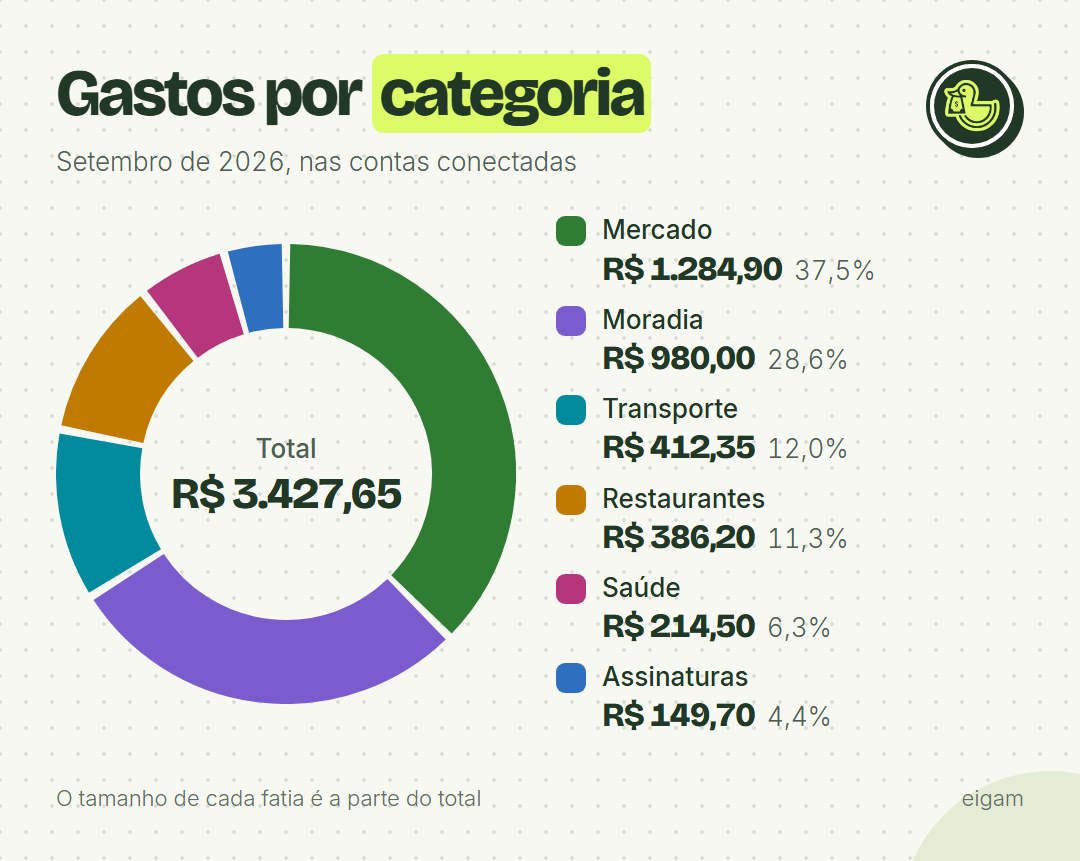
\includegraphics[width=\textwidth]{images/resultados/conversa_grafico_categorias.png}
        \authorssource
    \end{minipage}
    \hfill
    \begin{minipage}[t]{0.47\textwidth}
        \centering
        \caption{Gastos por banco na conversa}
        \label{fig:res_bancos}
        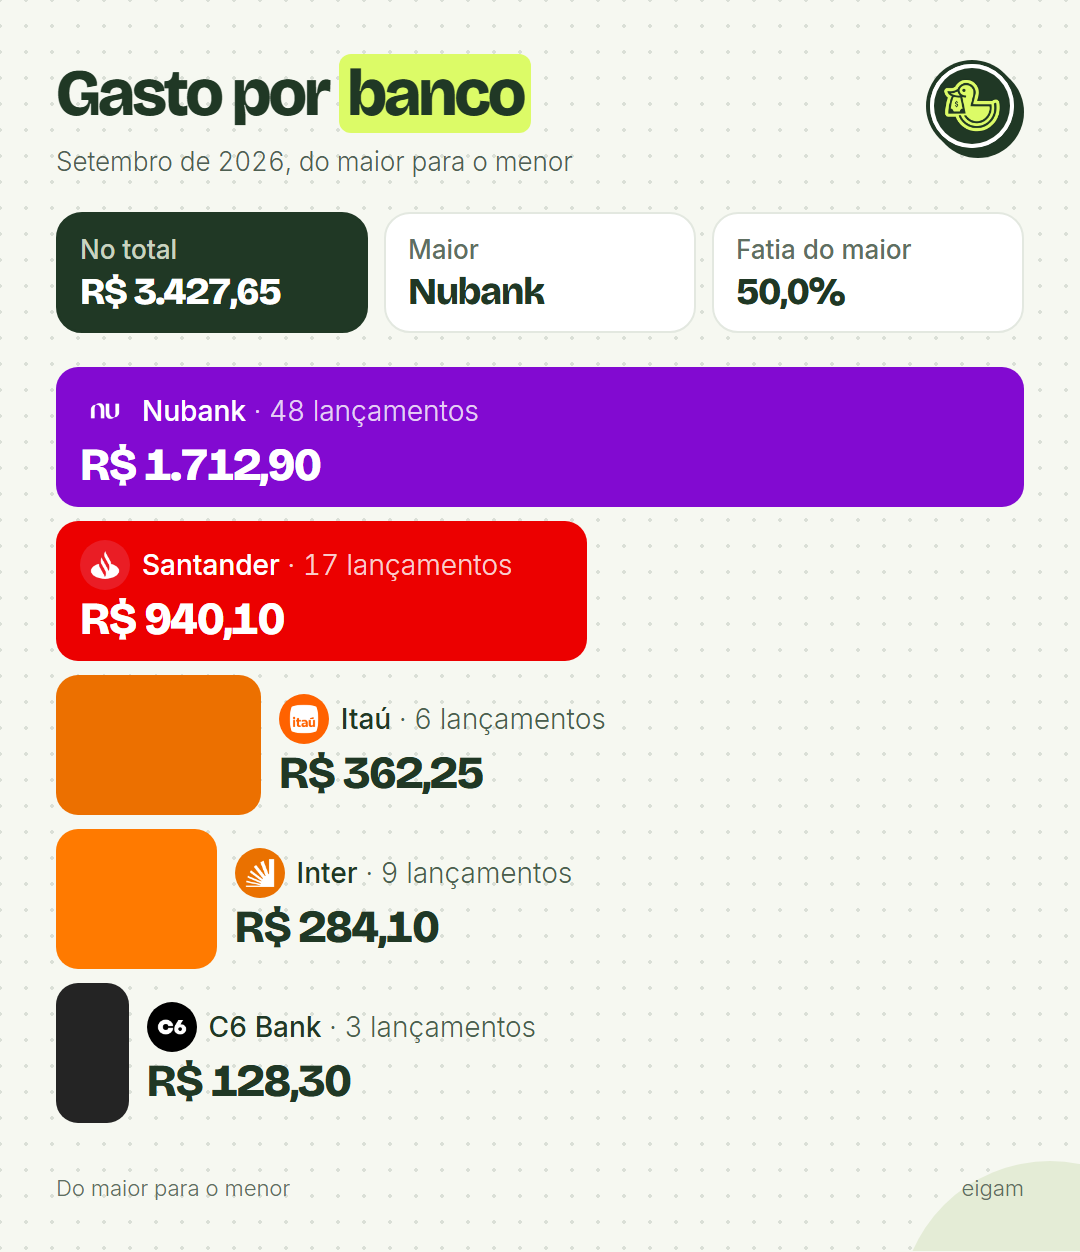
\includegraphics[width=\textwidth]{images/resultados/conversa_grafico_bancos.png}
        \authorssource
    \end{minipage}
\end{figure}

A Figura~\ref{fig:res_acumulado} compara o gasto acumulado do mês com o mesmo ponto do mês anterior, o que responde à pergunta ``estou gastando mais do que no mês passado?'' sem que o titular precise interpretar duas listas. A Figura~\ref{fig:res_comprovante} é o comprovante enviado quando uma conexão de \textit{Open Finance} é autorizada, com a instituição, a data e a validade escolhida pelo titular.

\begin{figure}[H]
    \centering
    \begin{minipage}[t]{0.47\textwidth}
        \centering
        \caption{Gasto acumulado contra o mês anterior}
        \label{fig:res_acumulado}
        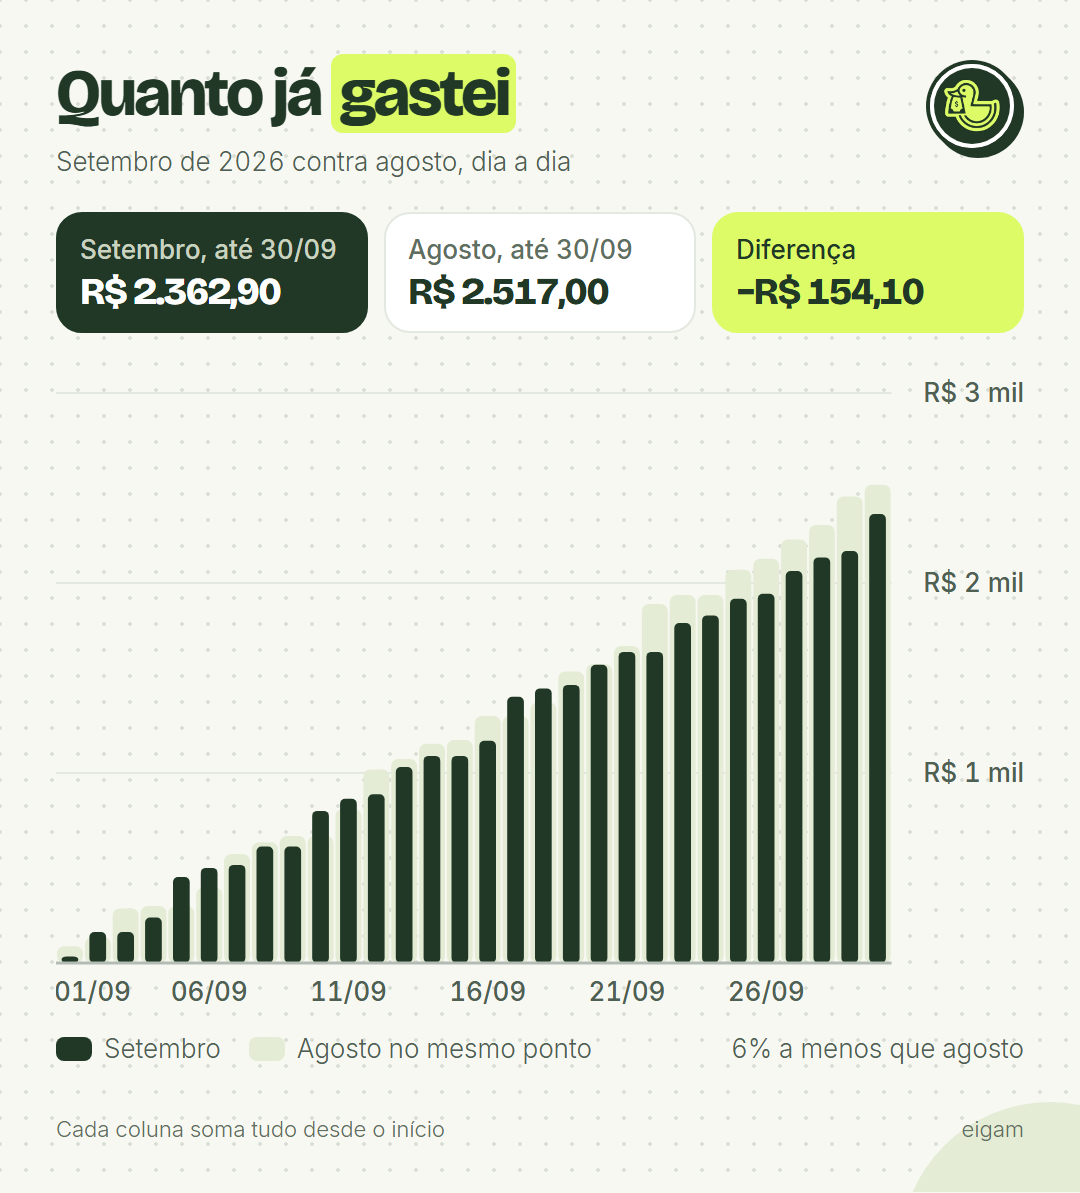
\includegraphics[width=\textwidth]{images/resultados/conversa_grafico_acumulado.png}
        \authorssource
    \end{minipage}
    \hfill
    \begin{minipage}[t]{0.47\textwidth}
        \centering
        \caption{Comprovante de conexão autorizada}
        \label{fig:res_comprovante}
        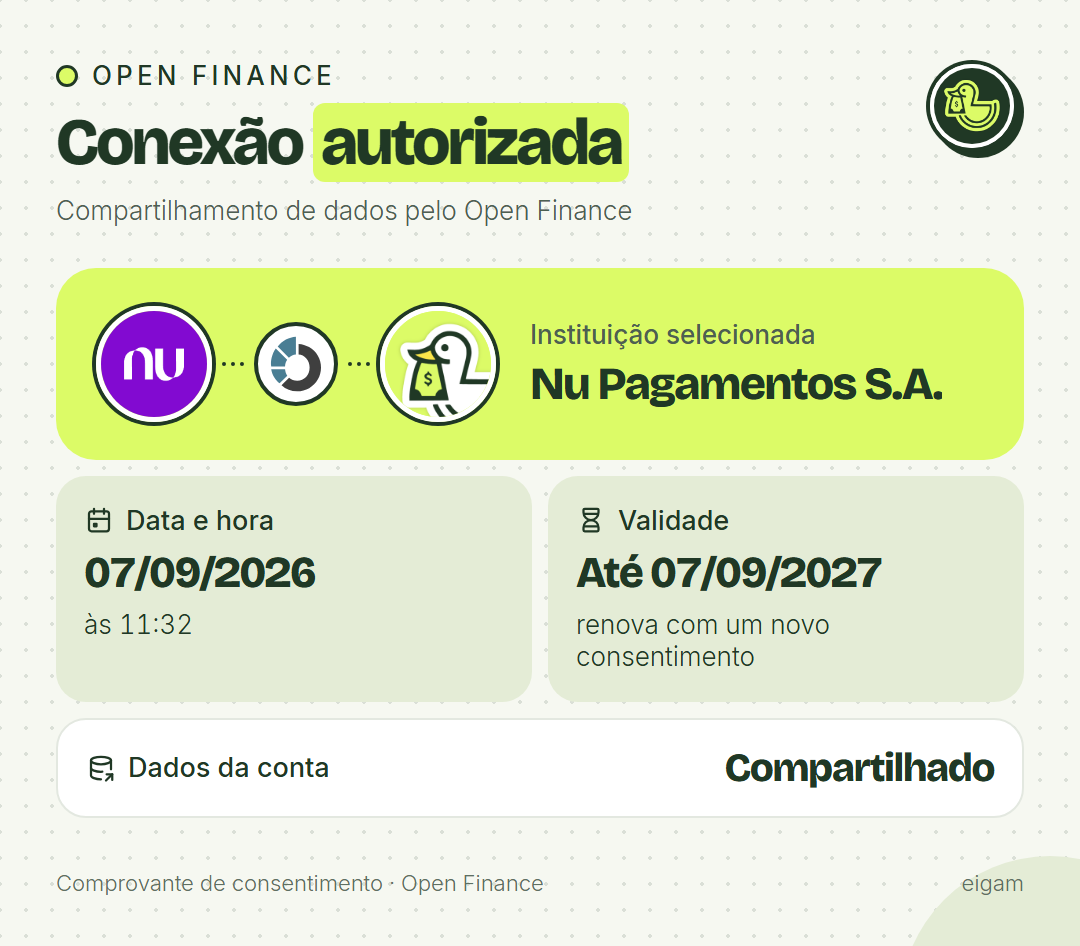
\includegraphics[width=\textwidth]{images/resultados/conversa_comprovante.png}
        \authorssource
    \end{minipage}
\end{figure}

A Figura~\ref{fig:res_com_pin} mostra uma resposta com o token de privilégio ativo, emitido depois do PIN. Sem o token, o sistema não gera imagens: os portões do gerador exigem valores liberados, e a resposta chega como texto com os valores mascarados em \texttt{R\$ •••••}, acompanhada da indicação de que o PIN libera os números. A decisão é do servidor, e não do modelo de linguagem.

\begin{figure}[H]
    \centering
    \caption{Resposta com imagem, emitida com o token de privilégio}
    \label{fig:res_com_pin}
    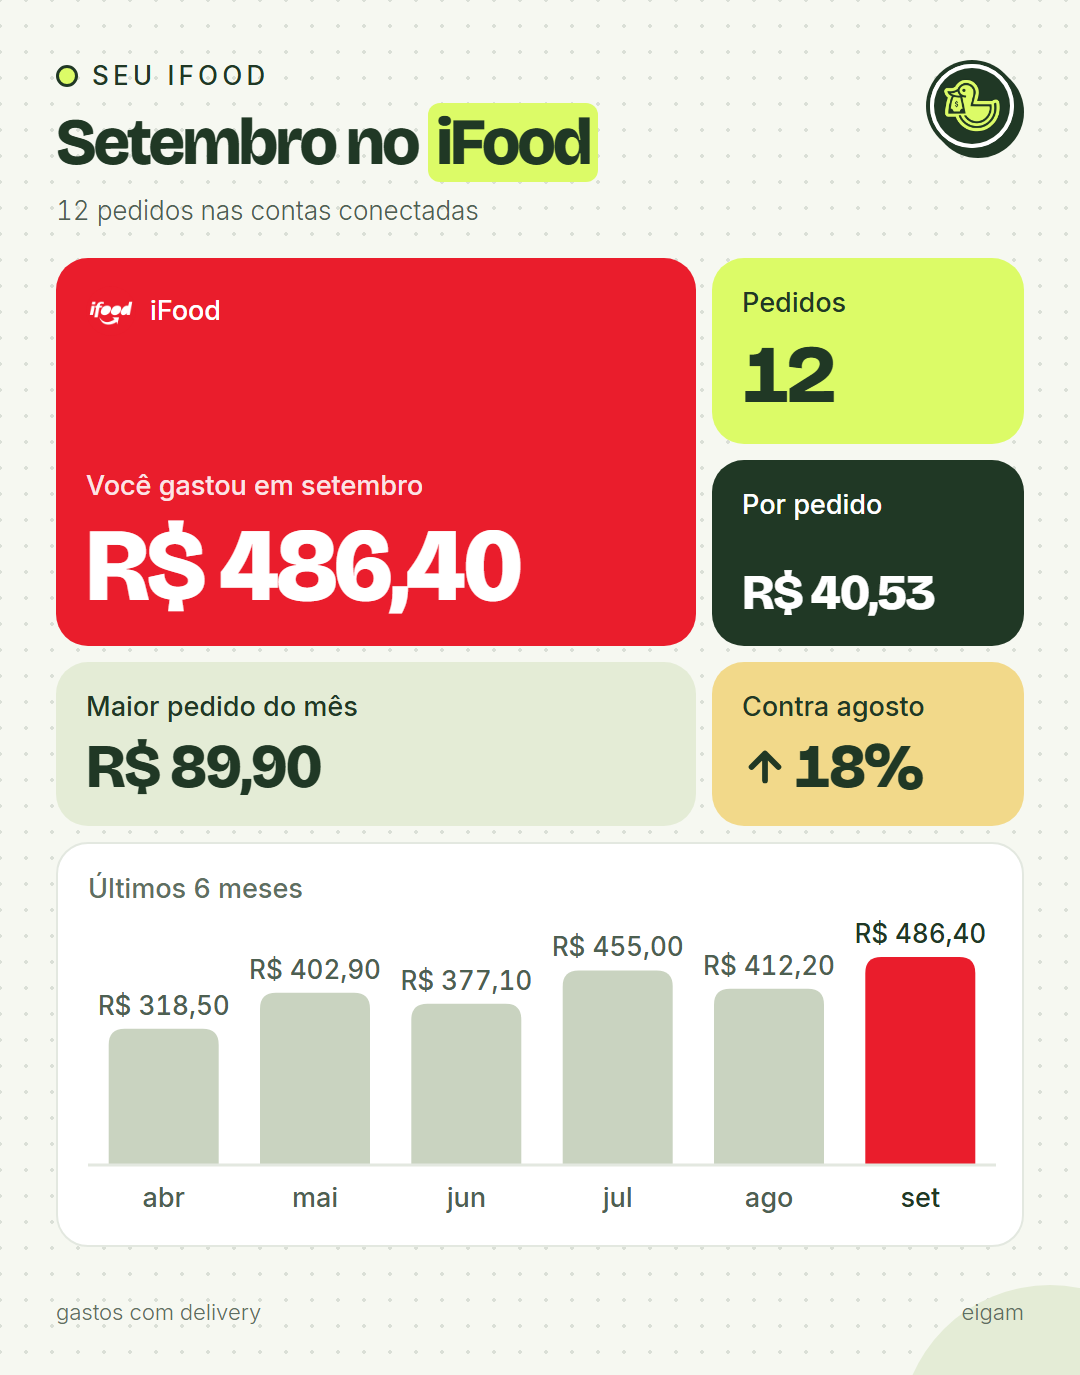
\includegraphics[width=0.6\textwidth]{images/resultados/conversa_app_com_pin.png}
    \authorssource
\end{figure}

\subsection{Fluxos Conversacionais}

As figuras desta seção percorrem, tela a tela, os principais processos conduzidos inteiramente pela conversa. Elas reproduzem conversas reais do beta, extraídas do histórico cifrado de conversas e apresentadas na interface do canal principal: os textos do sistema, os horários e os valores são os originais, e apenas nomes, CPF, e-mail, PIN e finais de cartão foram substituídos, de modo que nenhum titular pode ser identificado. As imagens são as que o próprio sistema enviou nessas conversas. Cada figura segue um único trecho contínuo, da primeira à última tela, e os cortes são indicados no texto. Os fluxos exercitam mecanismos distintos descritos no Capítulo~\ref{chap:desenvolvimento}: regras determinísticas, formulários guiados, o planejador, o mascaramento e as mensagens proativas.

O primeiro contato (Figura~\ref{fig:fluxo_inicio}) foi conduzido por regras determinísticas. A mensagem de boas-vindas apresentou o assistente, ofereceu respostas com uma conta de exemplo e pediu o aceite da Política de Privacidade e dos Termos de Uso antes de qualquer dado real. Depois do aceite e do nome, a titular perguntou o gasto do mês e recebeu a resposta calculada sobre a conta de demonstração, identificada como tal, sem ter informado CPF nem conectado banco.

\begin{figure}[H]
    \centering
    \caption{Primeiro contato e conta de exemplo}
    \label{fig:fluxo_inicio}
    \begin{minipage}[t]{0.32\textwidth}
        \centering
        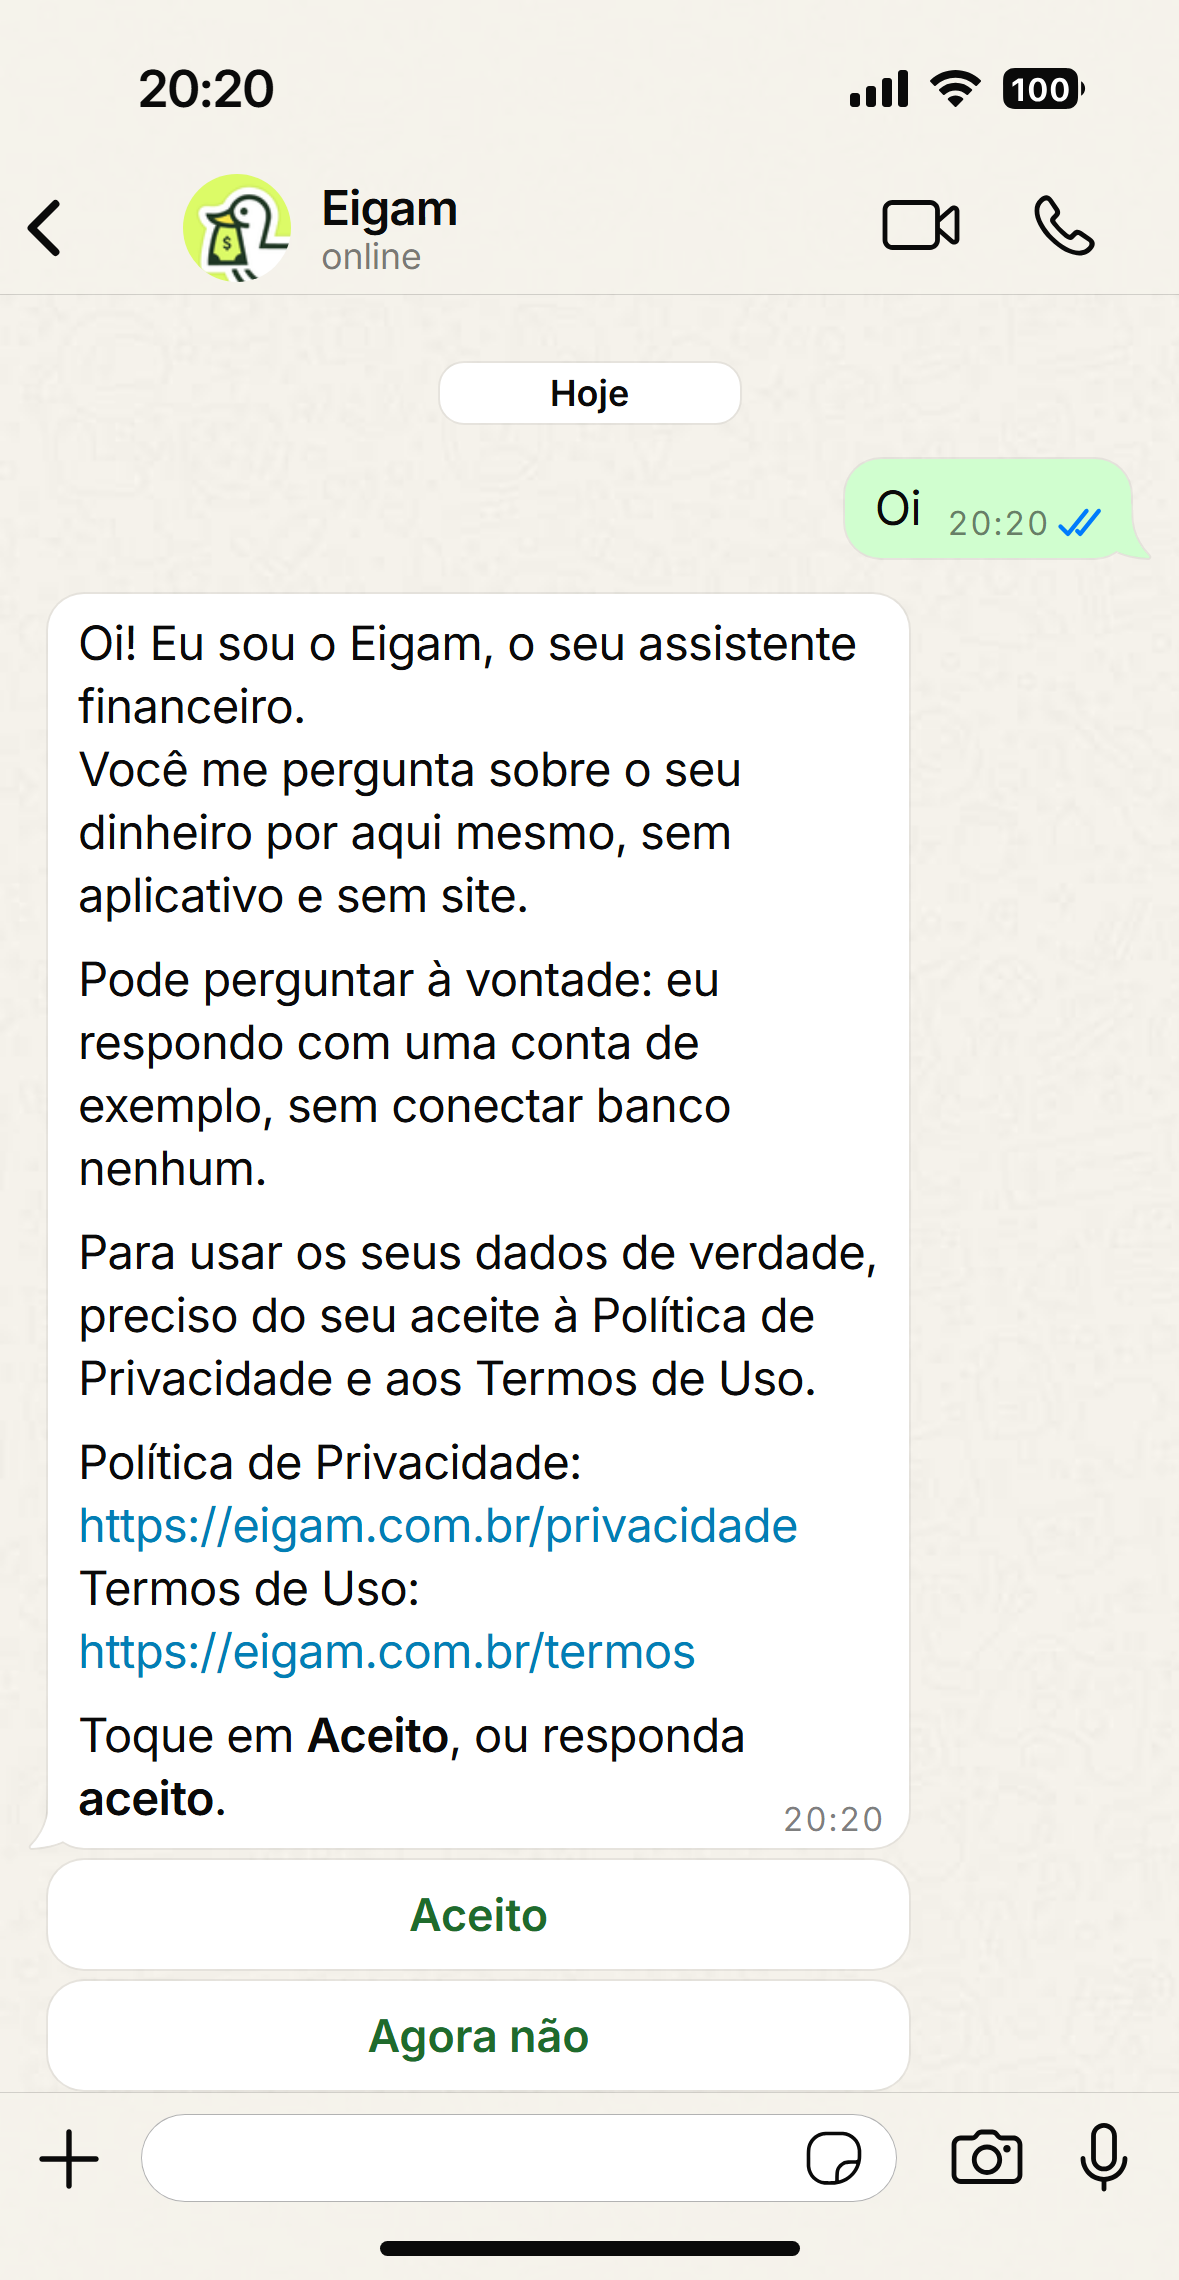
\includegraphics[width=\textwidth]{images/resultados/fluxos/fluxo_inicio_a.png}
    \end{minipage}\hfill
    \begin{minipage}[t]{0.32\textwidth}
        \centering
        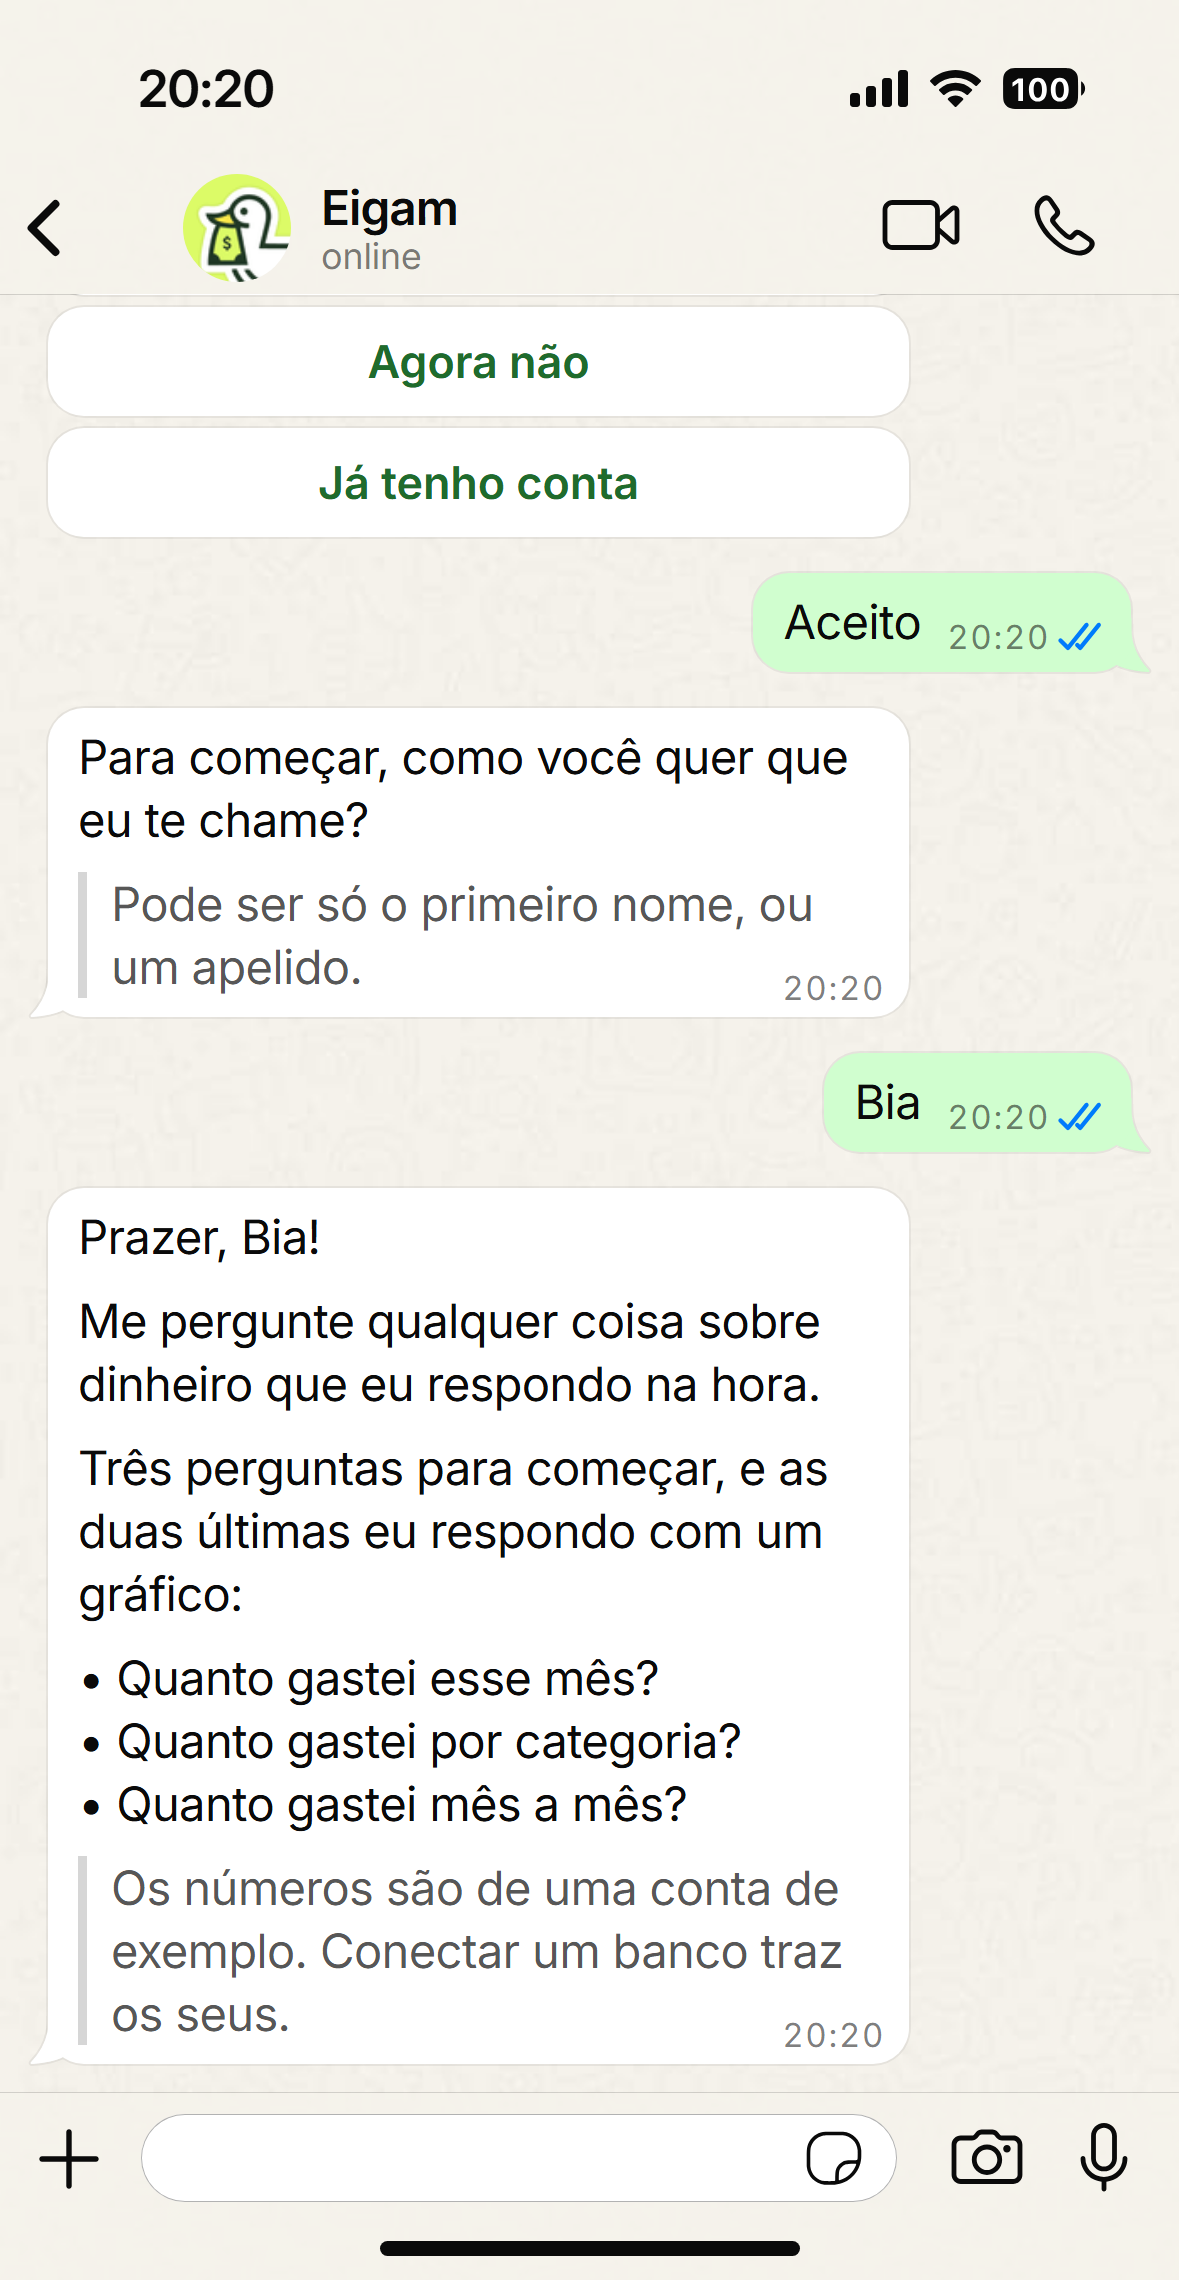
\includegraphics[width=\textwidth]{images/resultados/fluxos/fluxo_inicio_b.png}
    \end{minipage}\hfill
    \begin{minipage}[t]{0.32\textwidth}
        \centering
        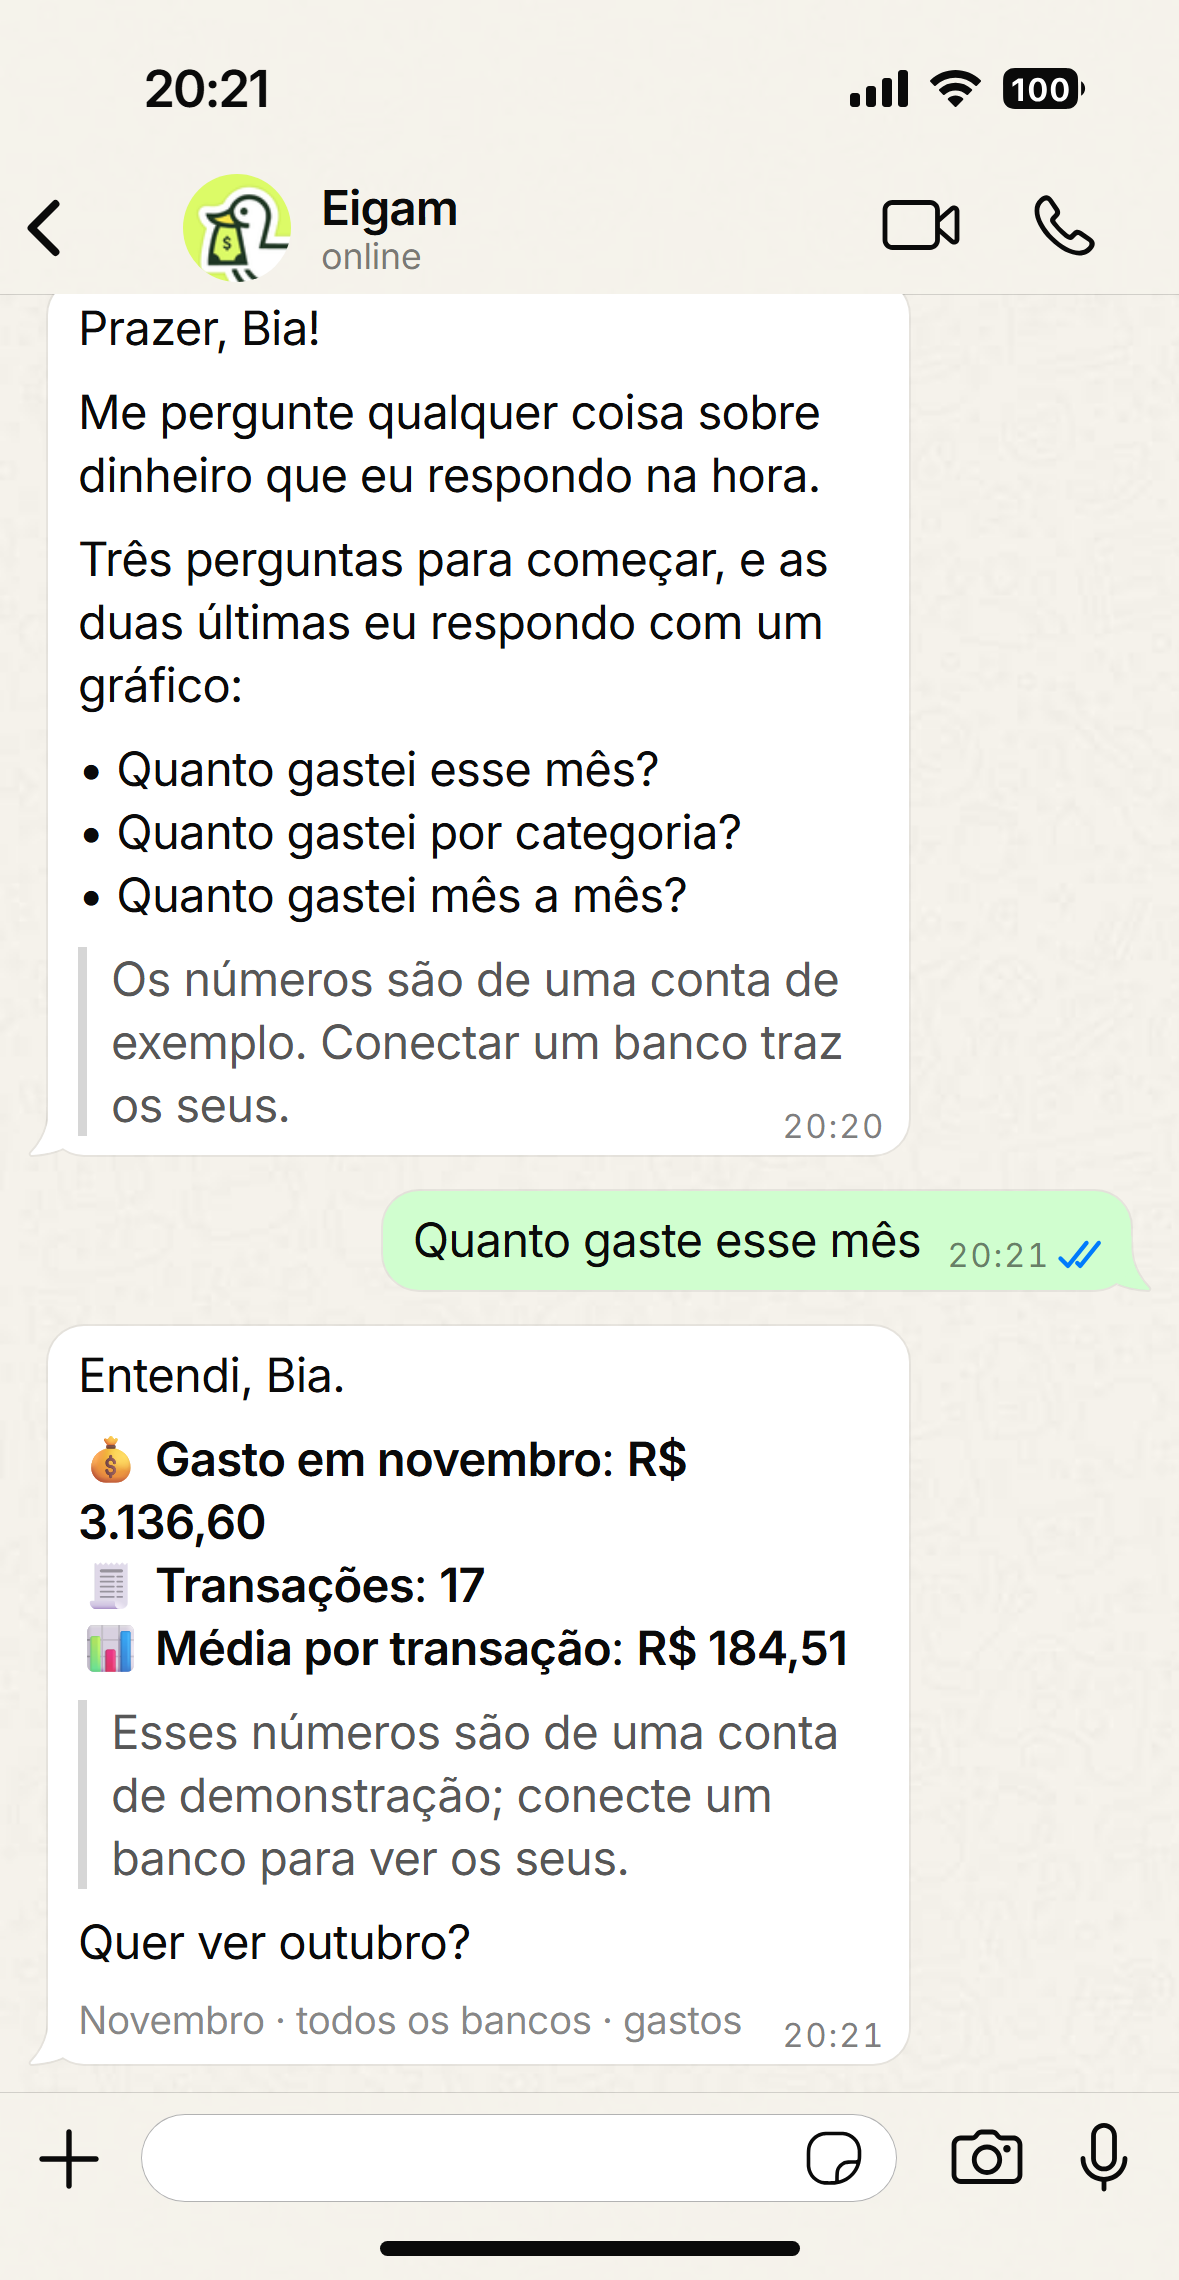
\includegraphics[width=\textwidth]{images/resultados/fluxos/fluxo_inicio_c.png}
    \end{minipage}
    \authorssource
\end{figure}

O cadastro (Figura~\ref{fig:fluxo_cadastro}) começou, na mesma conversa, quando a titular pediu para conectar um banco. Como a conexão pelo \textit{Open Finance} exige o CPF, o sistema explicou o que faltava e por quê, e conduziu a coleta de CPF, e-mail e PIN de seis dígitos, com a repetição do PIN para confirmação. Esses dados não ficaram no histórico: o registro da conversa guarda apenas a marca de dado sigiloso omitido, e o PIN é armazenado somente como \textit{hash}. Ao final, o botão já levava ao banco escolhido no início do pedido.

\begin{figure}[H]
    \centering
    \caption{Fluxo de cadastro pela conversa}
    \label{fig:fluxo_cadastro}
    \begin{minipage}[t]{0.32\textwidth}
        \centering
        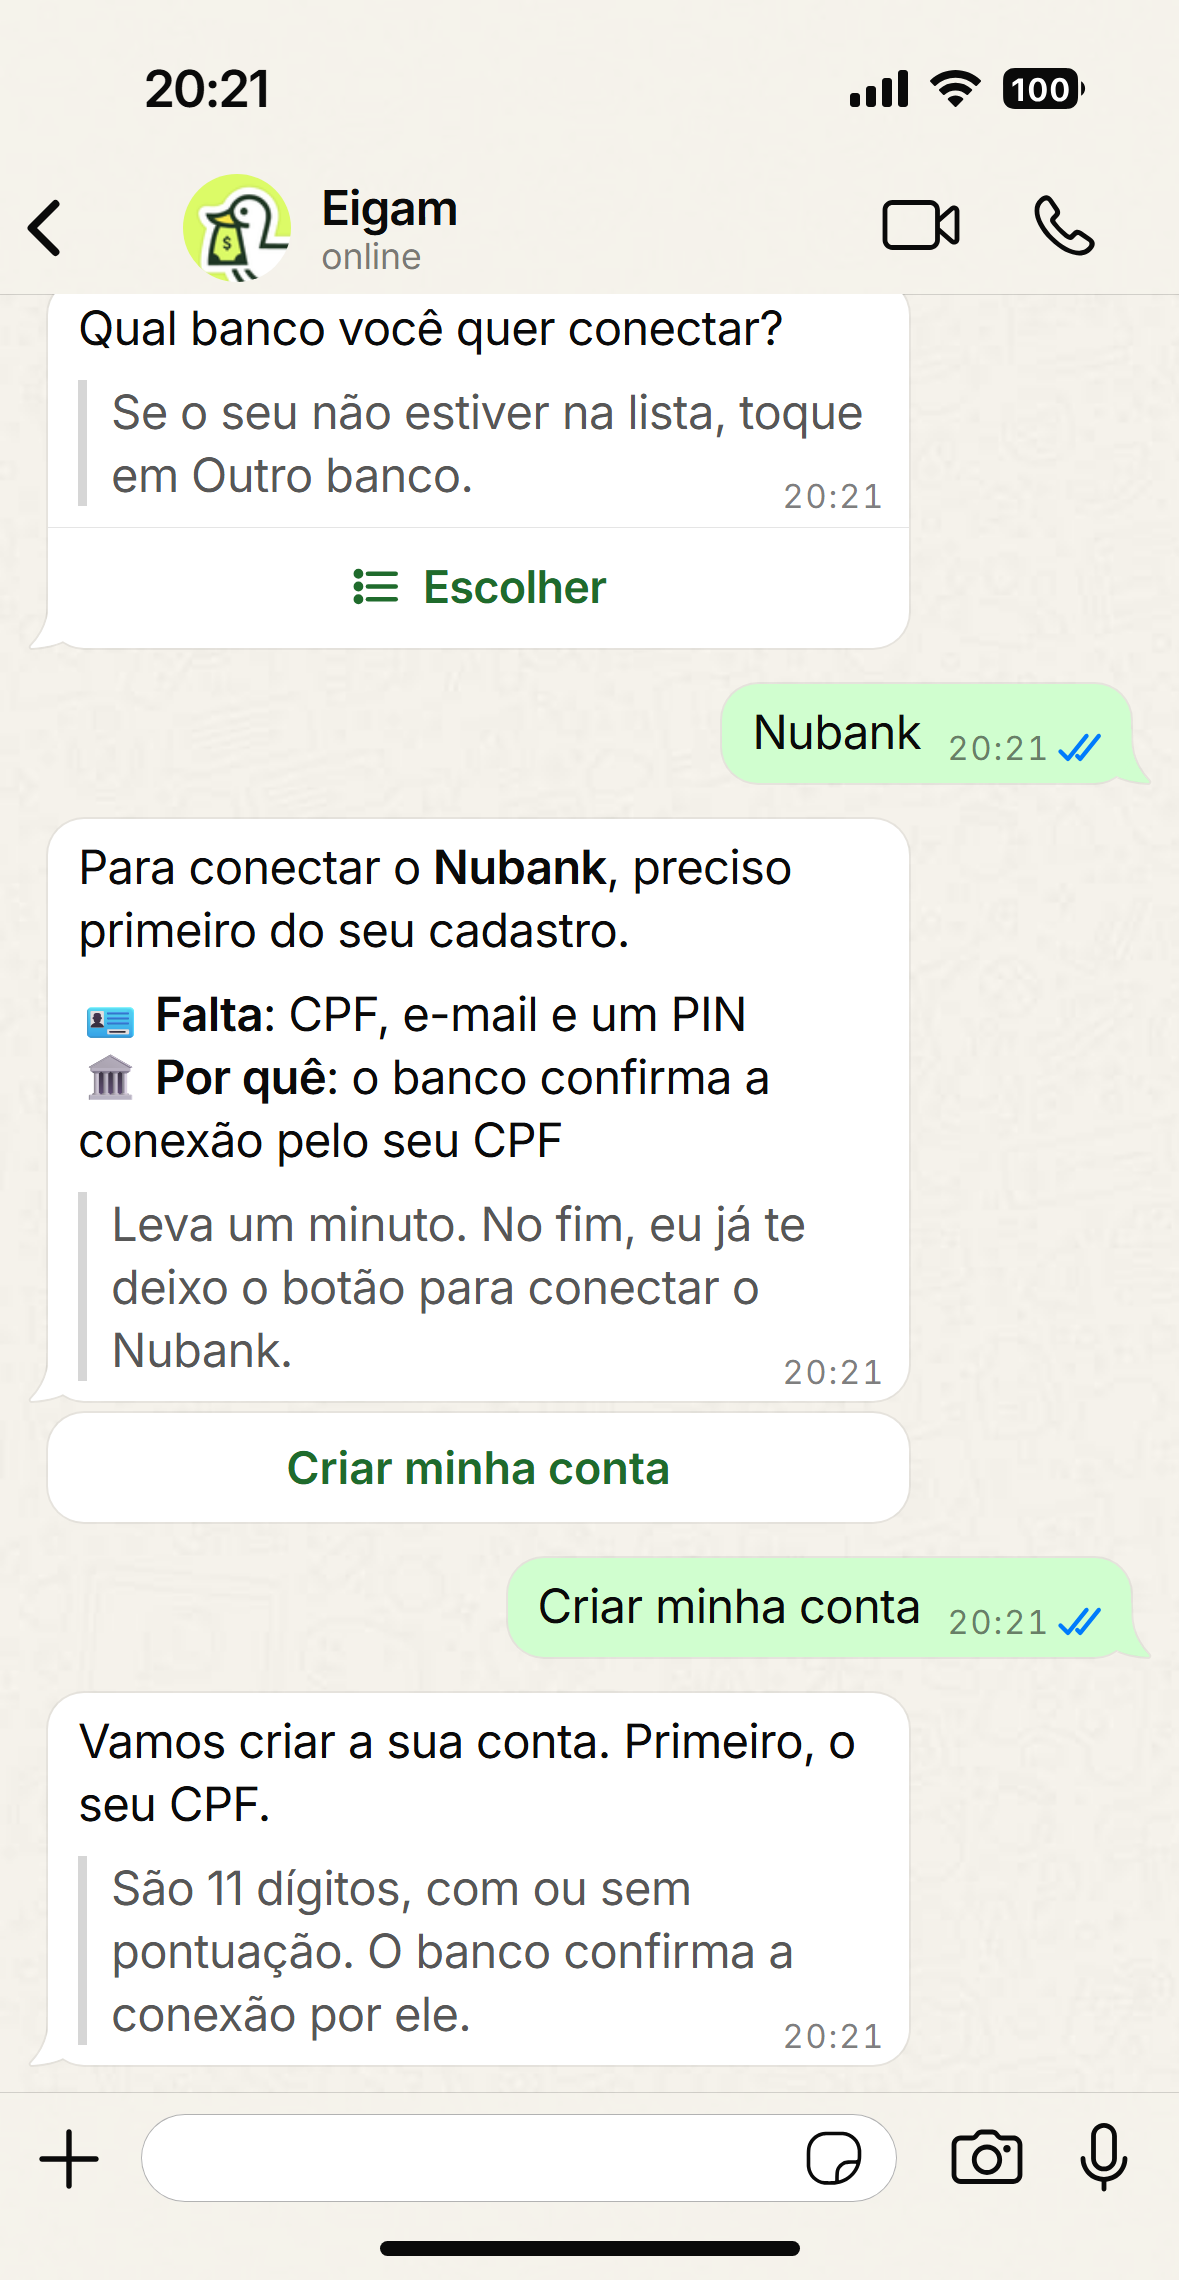
\includegraphics[width=\textwidth]{images/resultados/fluxos/fluxo_cadastro_a.png}
    \end{minipage}\hfill
    \begin{minipage}[t]{0.32\textwidth}
        \centering
        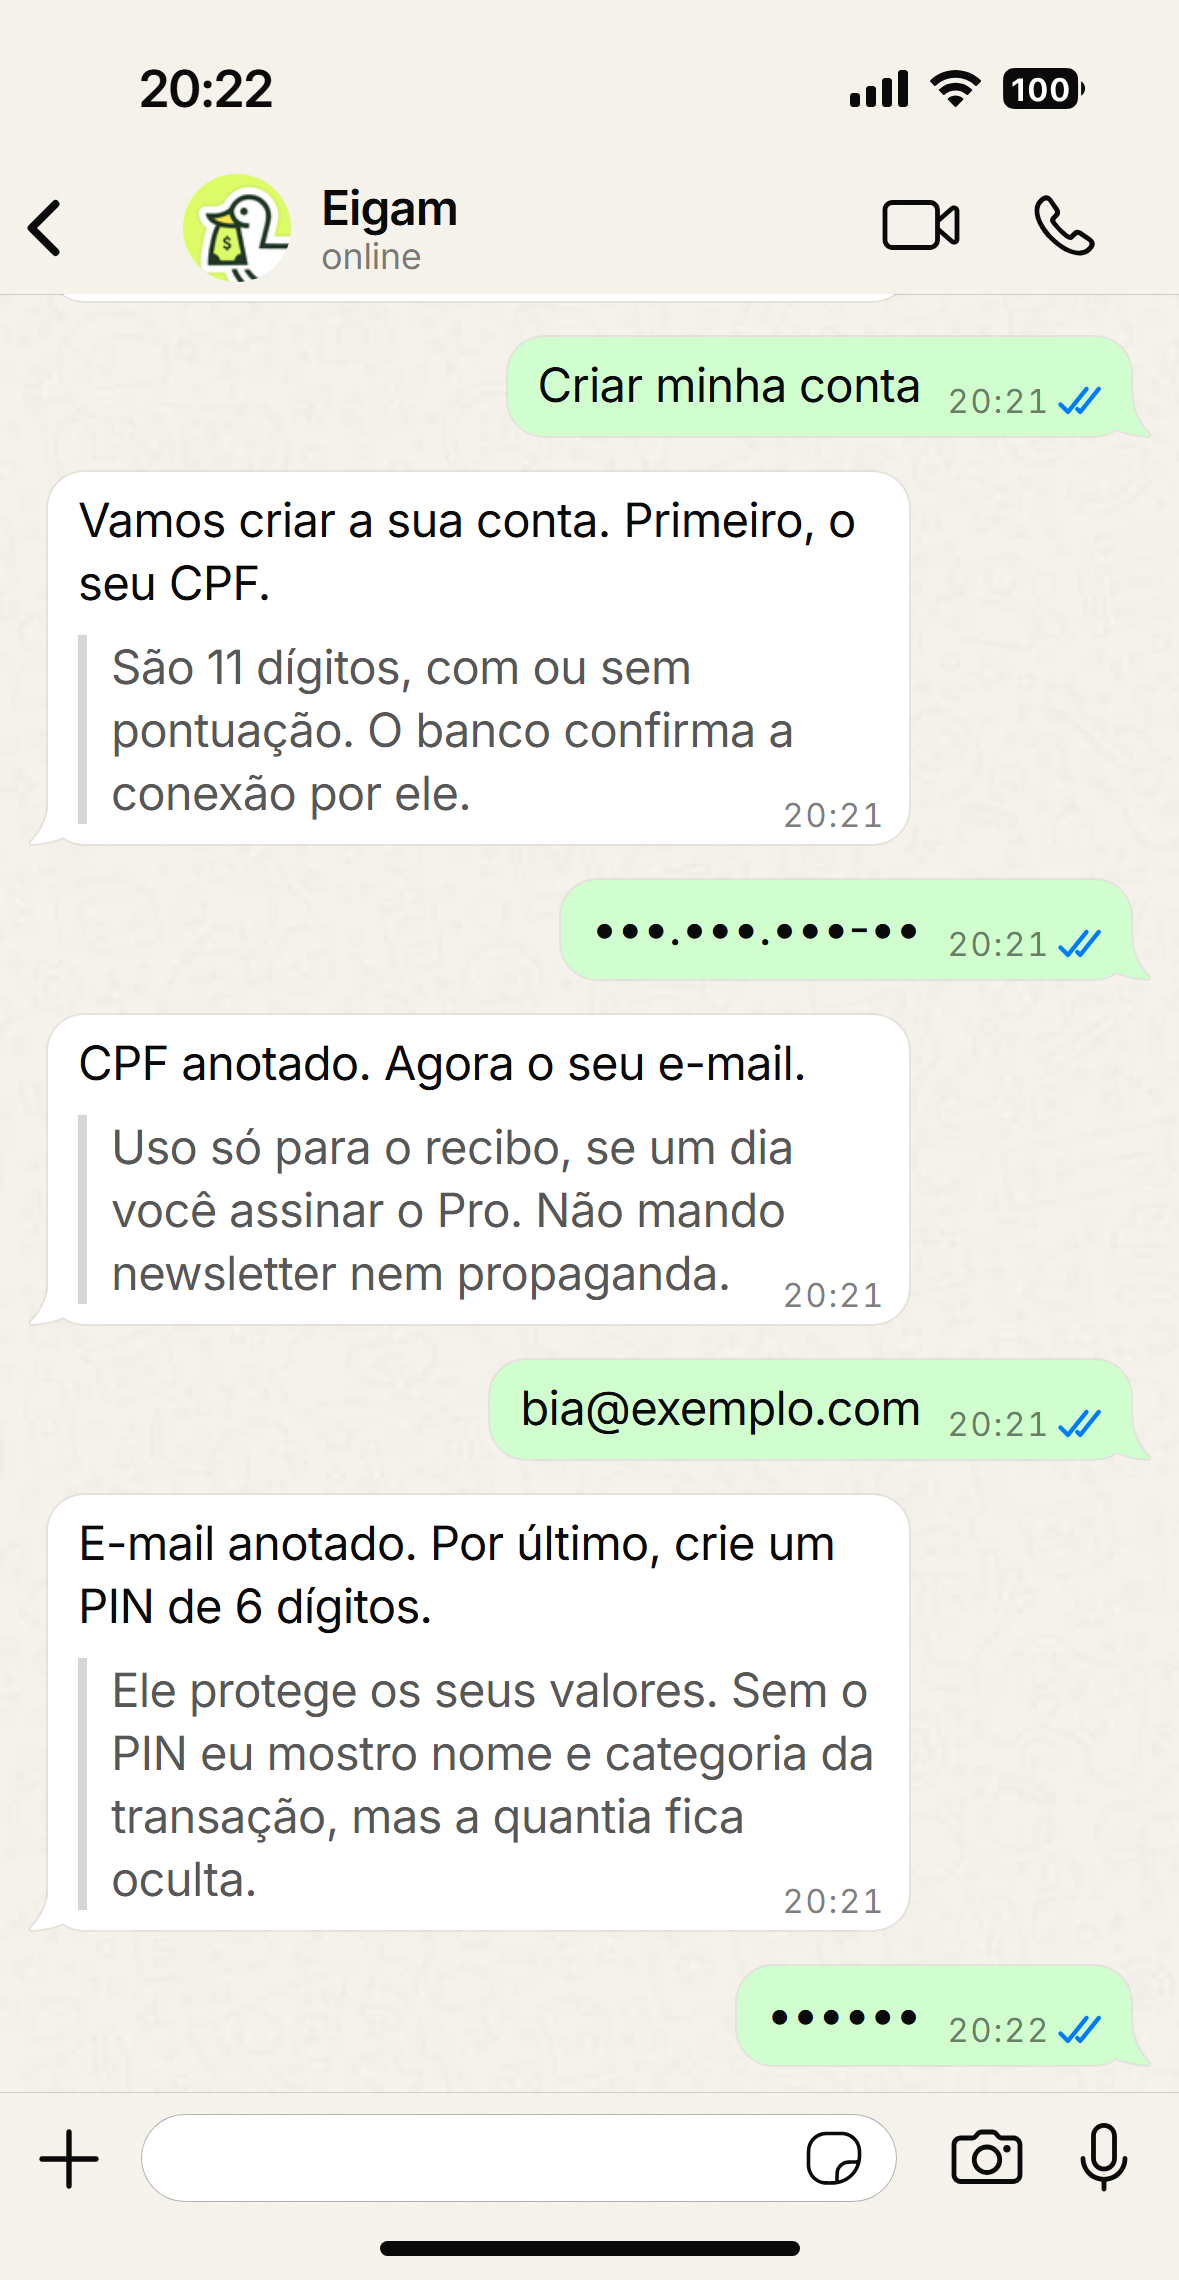
\includegraphics[width=\textwidth]{images/resultados/fluxos/fluxo_cadastro_b.png}
    \end{minipage}\hfill
    \begin{minipage}[t]{0.32\textwidth}
        \centering
        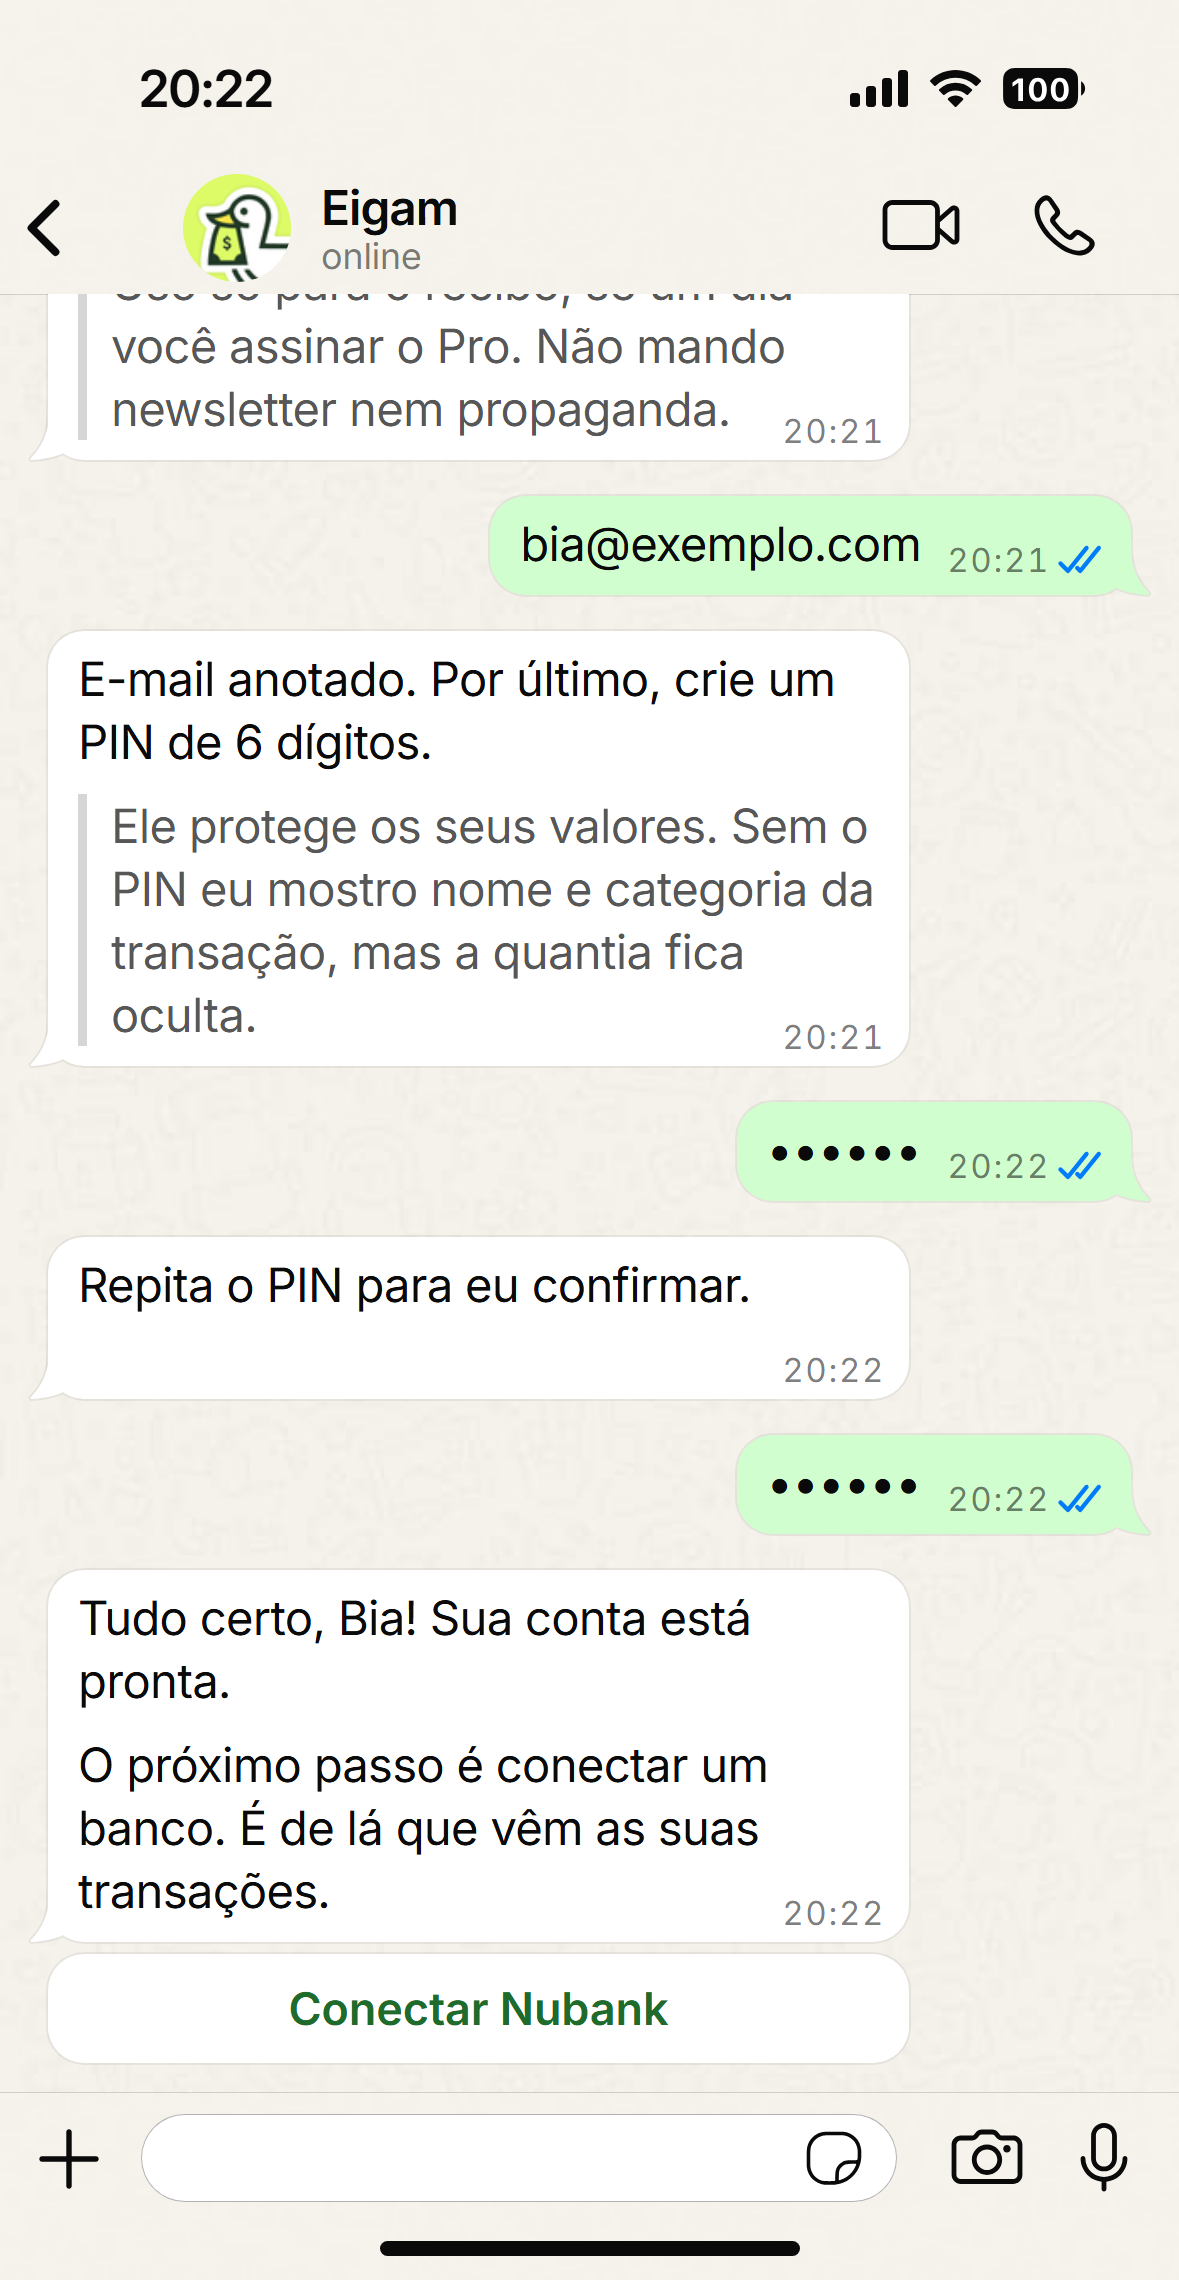
\includegraphics[width=\textwidth]{images/resultados/fluxos/fluxo_cadastro_c.png}
    \end{minipage}
    \authorssource
\end{figure}

A conexão de banco (Figura~\ref{fig:fluxo_banco}) partiu de um titular que já tinha três instituições conectadas. Como a instituição desejada não estava entre os atalhos da lista, ele a indicou em um formulário; a autorização aconteceu no aplicativo do próprio banco, sem que a senha bancária passasse pela solução, e cerca de um minuto depois chegou o comprovante de consentimento, com a instituição, a data, a hora e a validade, junto da quantidade de transações encontradas. Os valores dessas transações permaneceram ocultos até o PIN.

\begin{figure}[H]
    \centering
    \caption{Fluxo de conexão de banco pelo \textit{Open Finance}}
    \label{fig:fluxo_banco}
    \begin{minipage}[t]{0.32\textwidth}
        \centering
        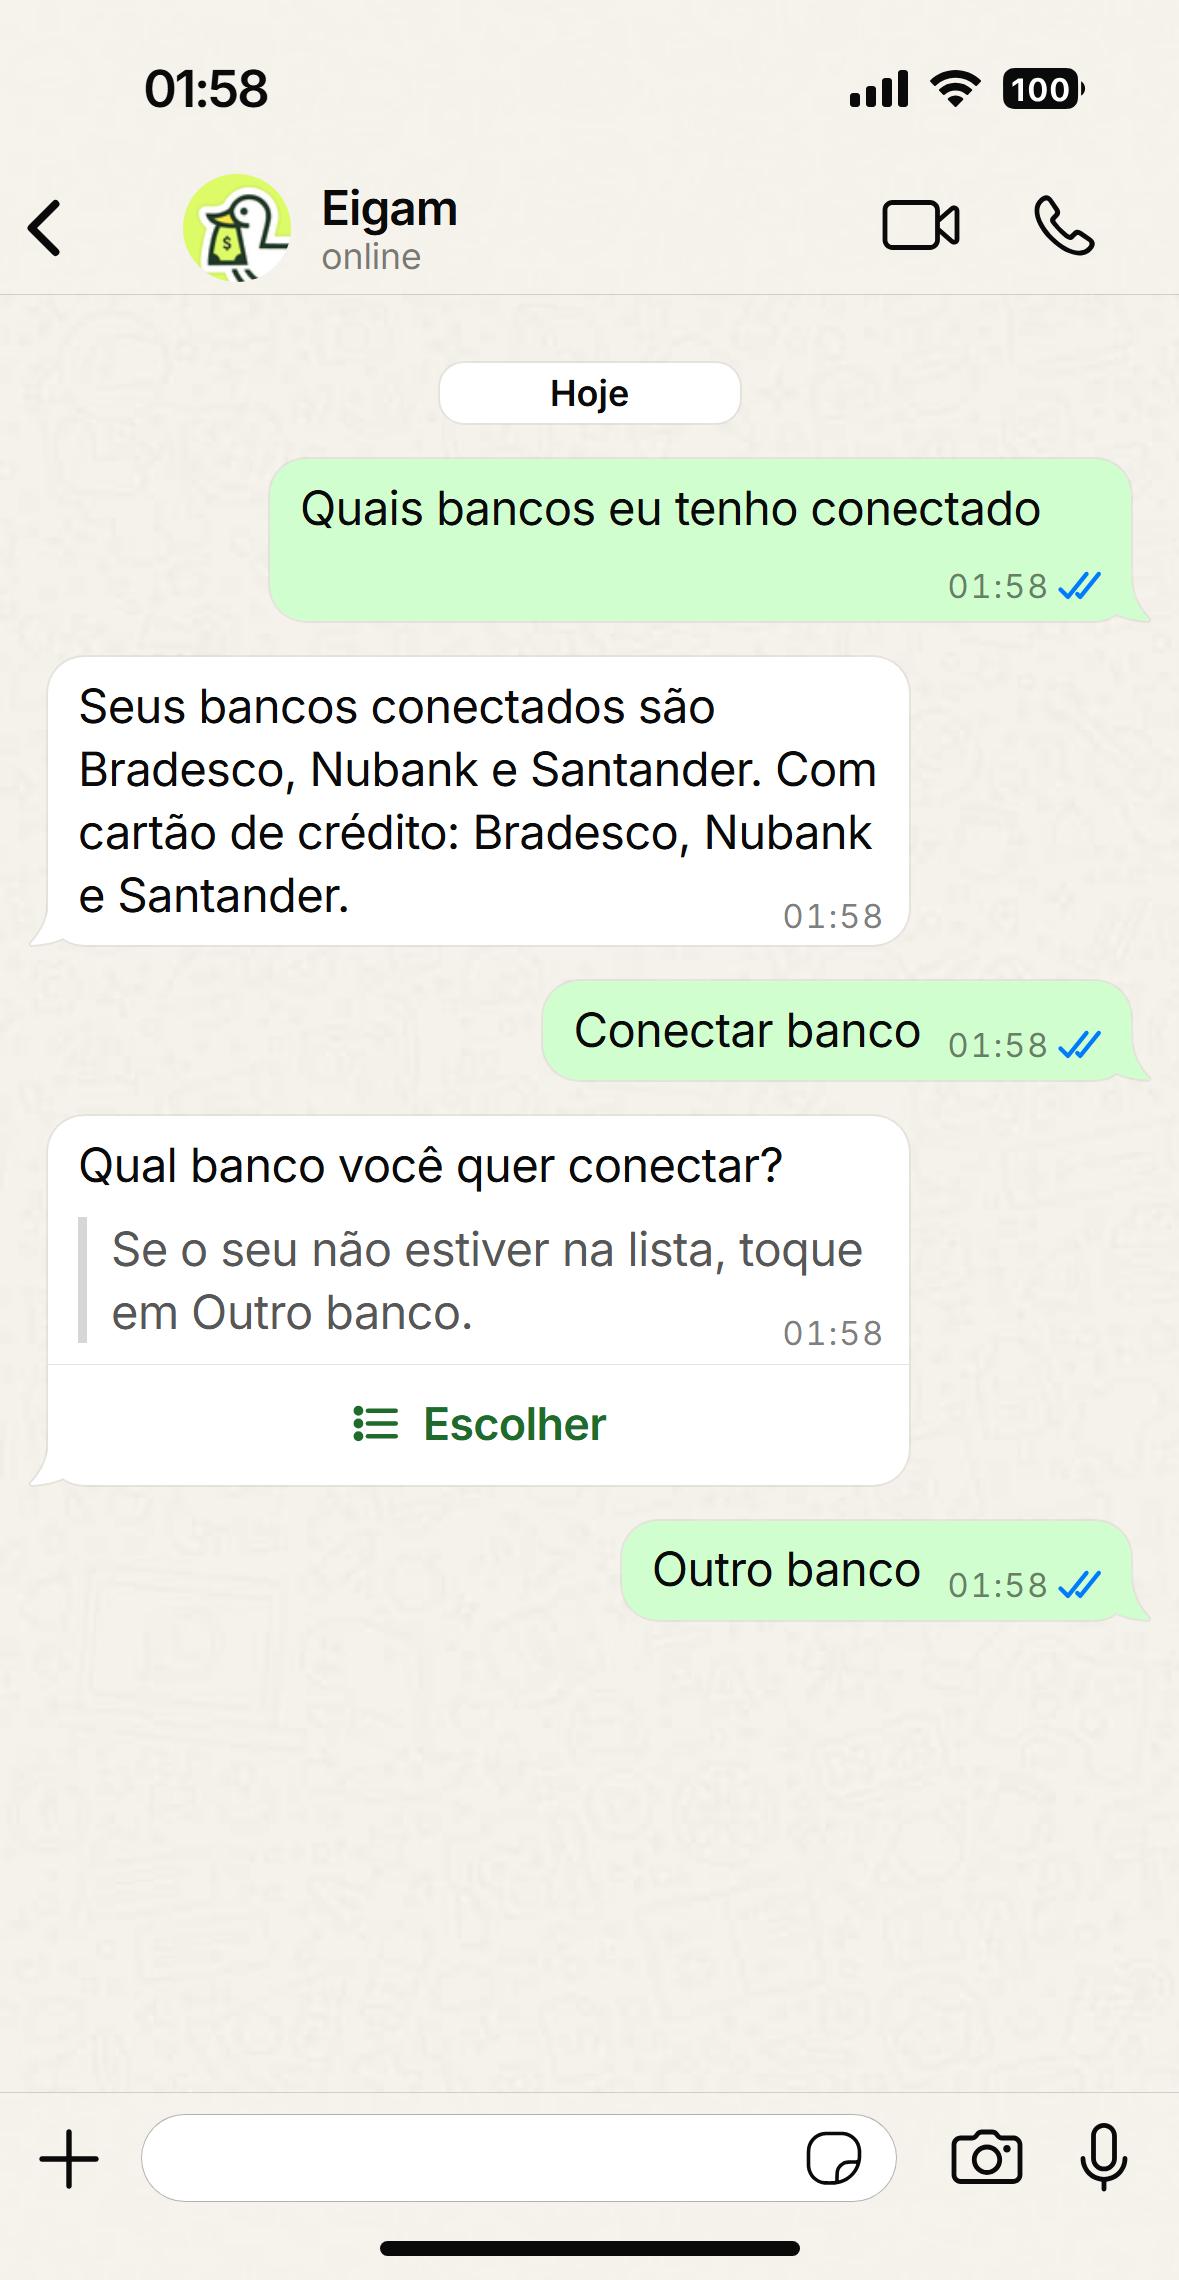
\includegraphics[width=\textwidth]{images/resultados/fluxos/fluxo_banco_a.png}
    \end{minipage}\hfill
    \begin{minipage}[t]{0.32\textwidth}
        \centering
        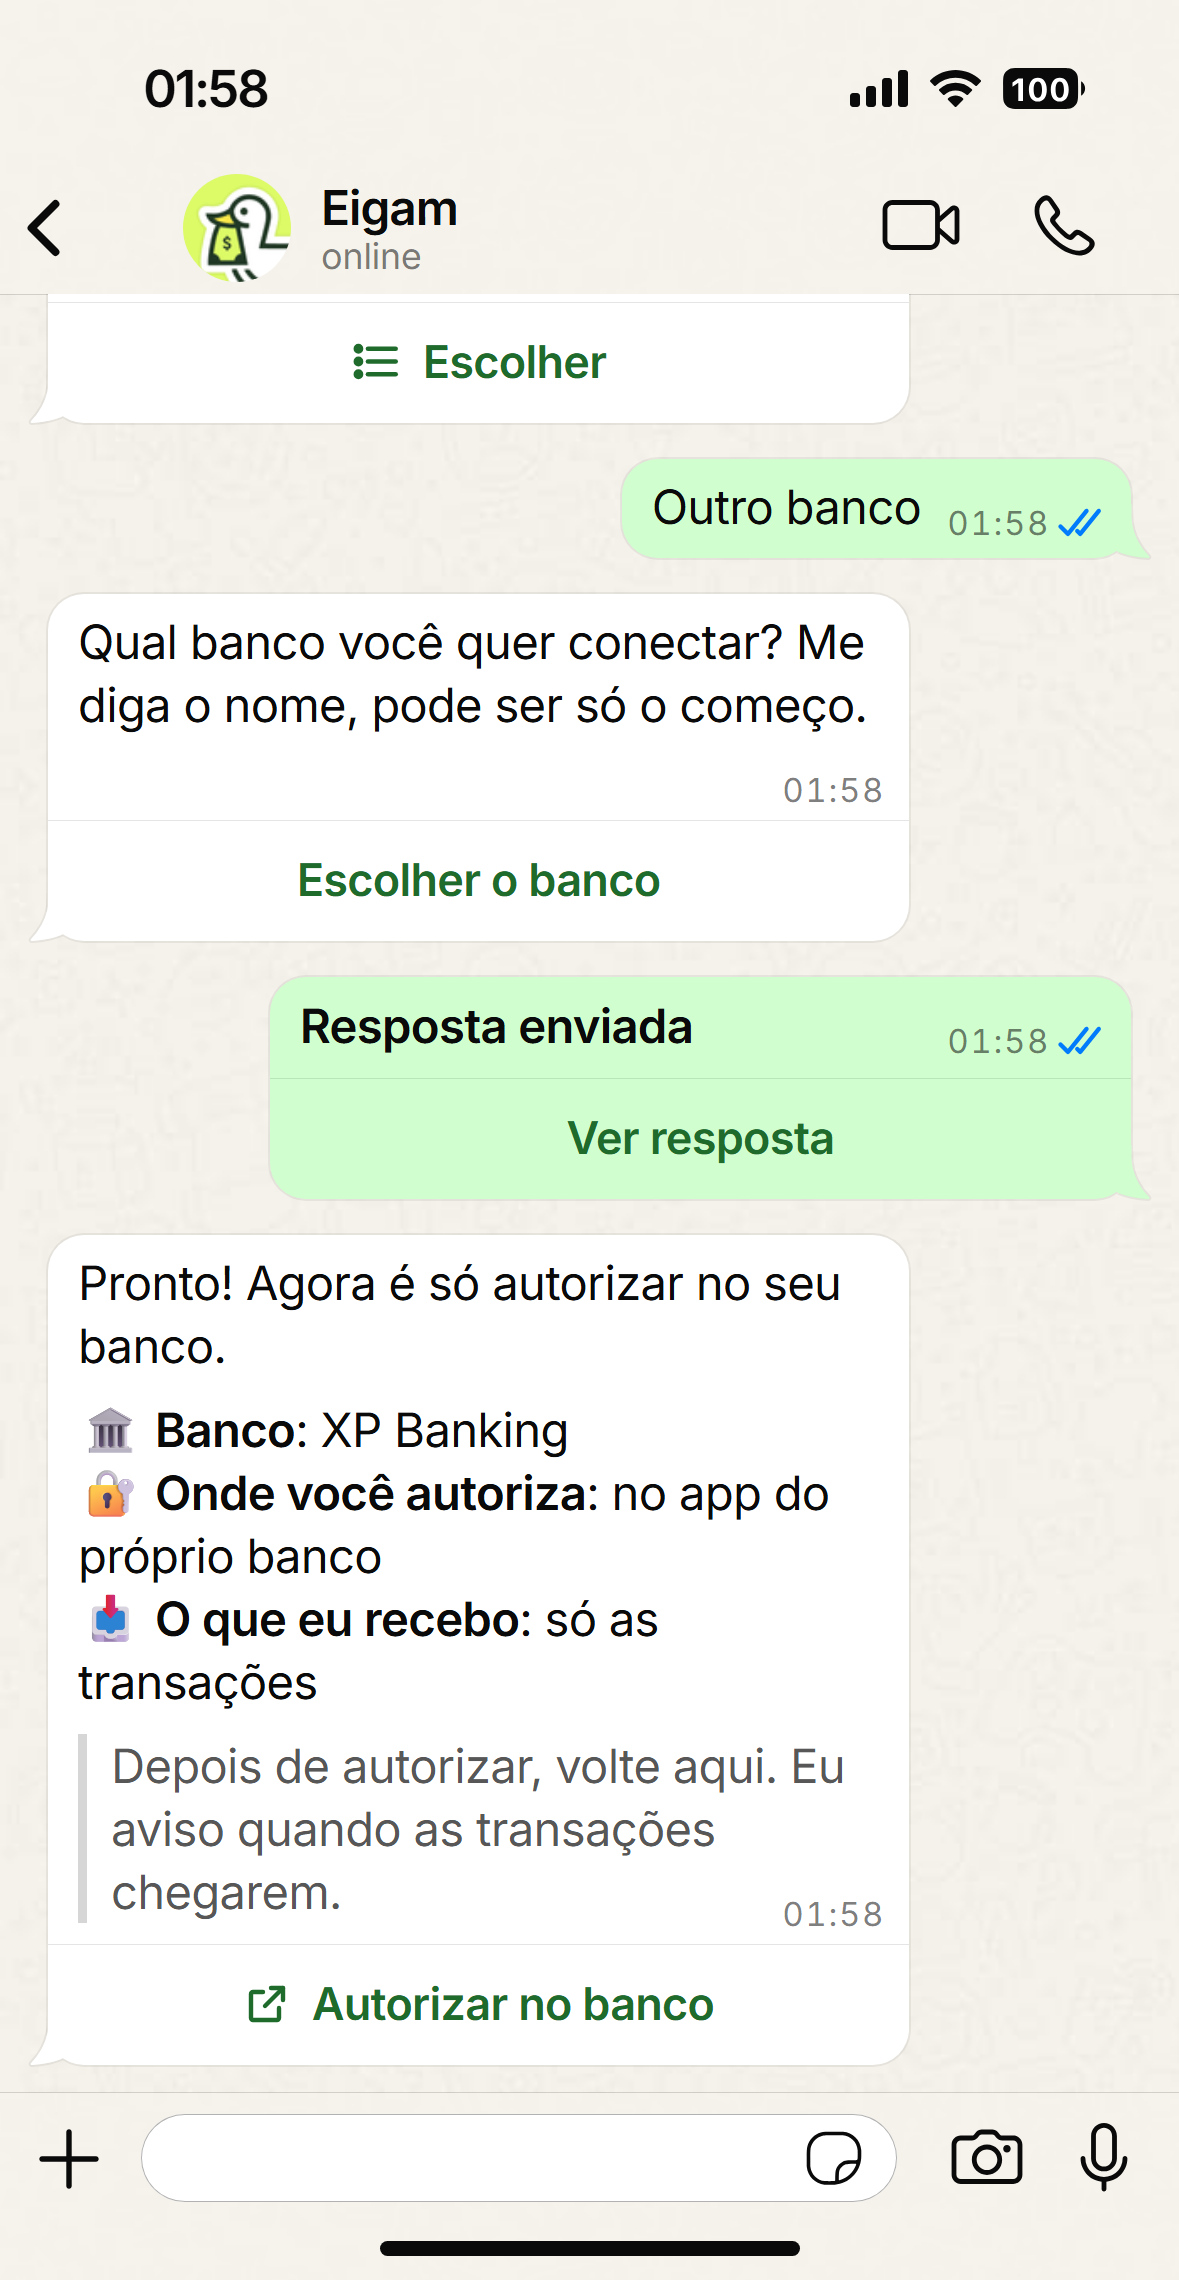
\includegraphics[width=\textwidth]{images/resultados/fluxos/fluxo_banco_b.png}
    \end{minipage}\hfill
    \begin{minipage}[t]{0.32\textwidth}
        \centering
        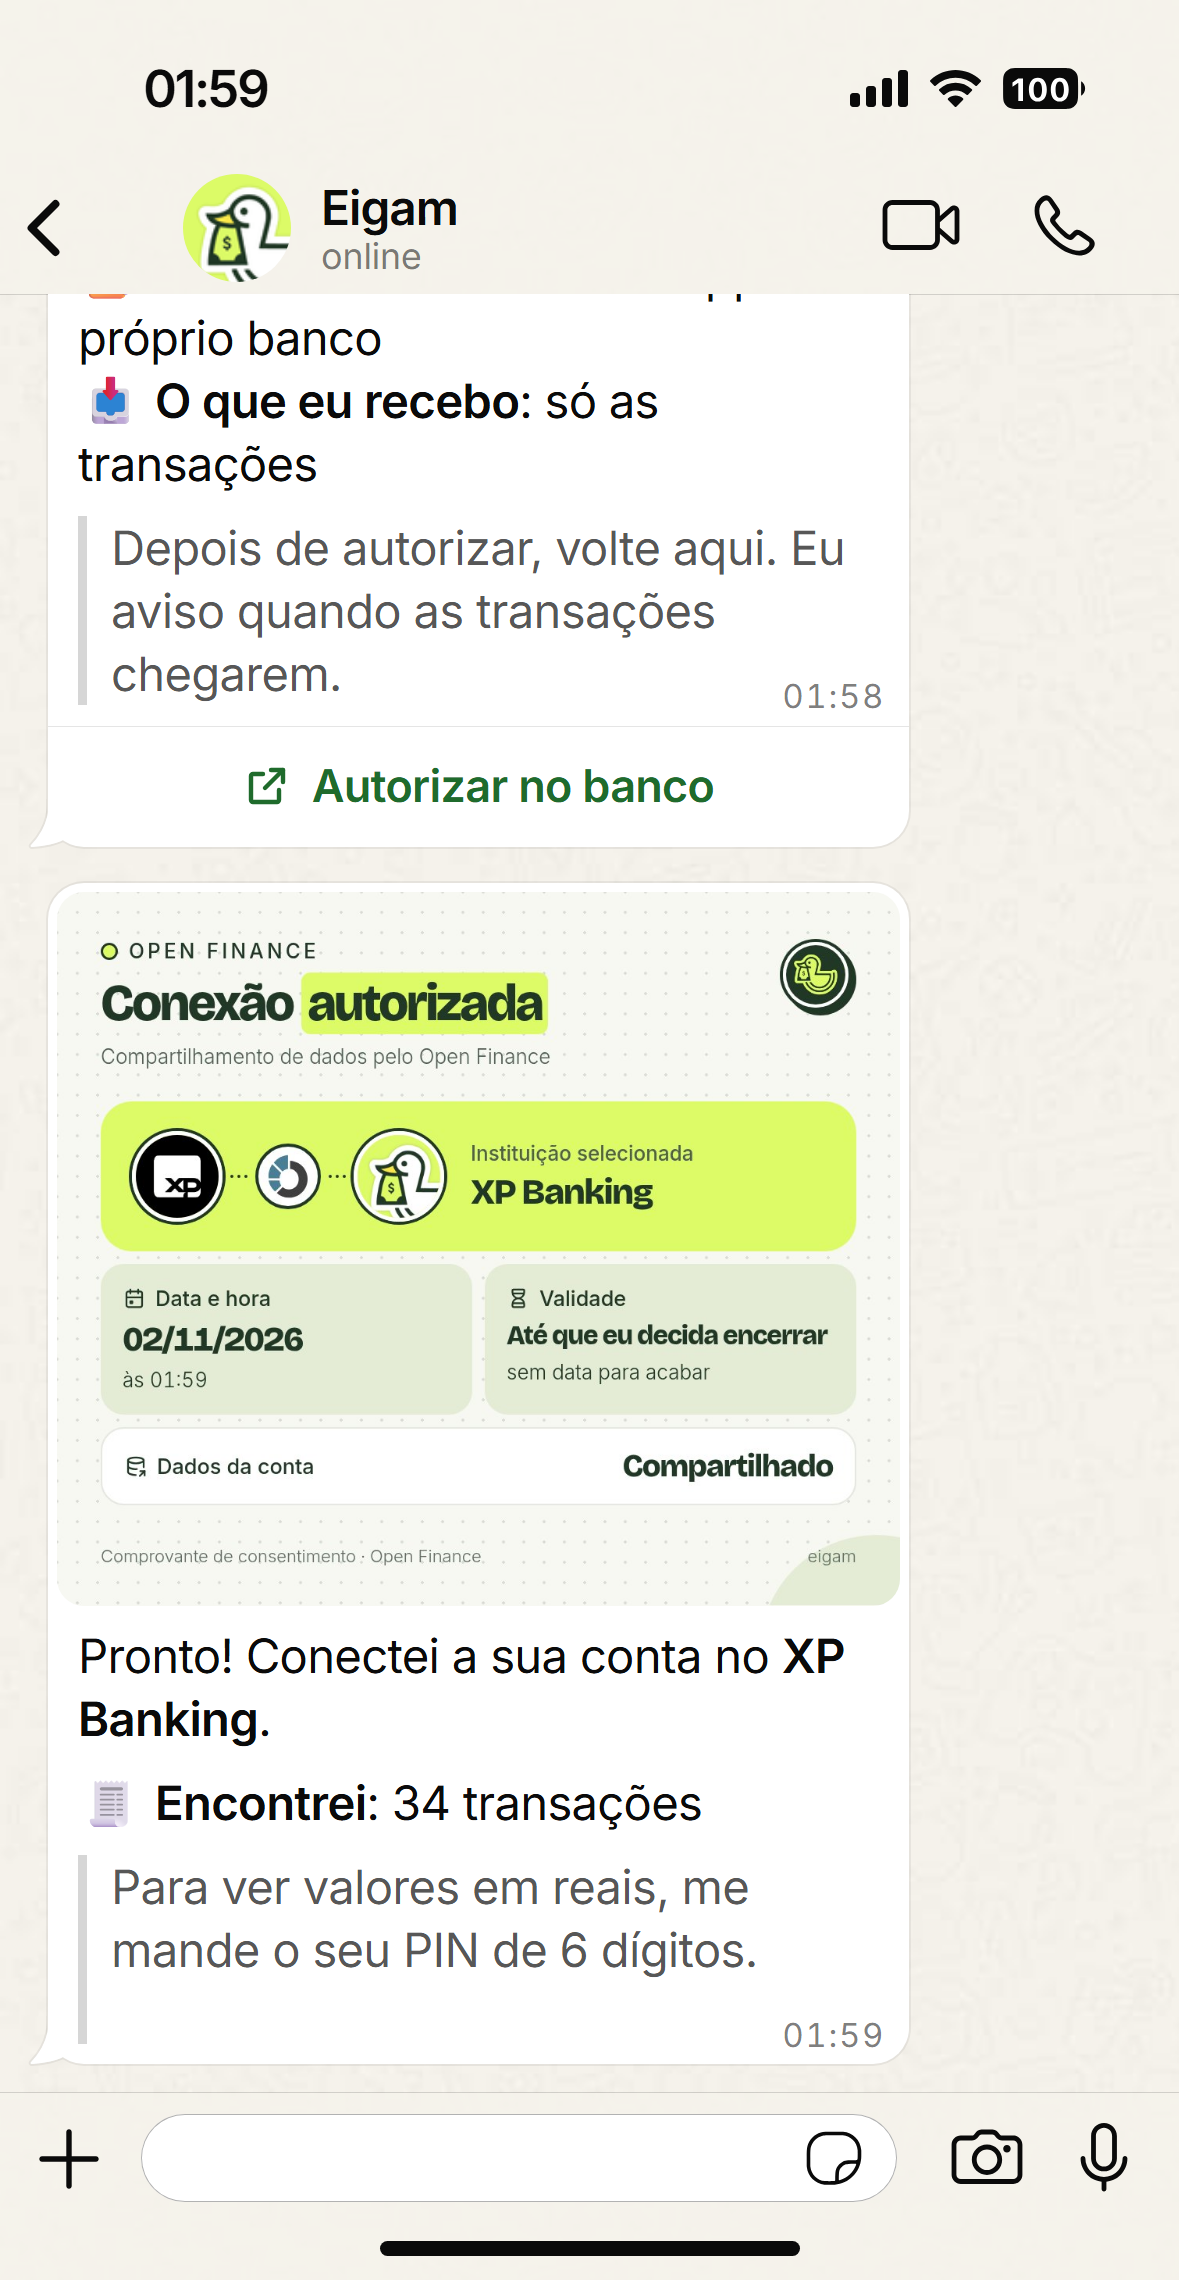
\includegraphics[width=\textwidth]{images/resultados/fluxos/fluxo_banco_c.png}
    \end{minipage}
    \authorssource
\end{figure}

A consulta financeira (Figura~\ref{fig:fluxo_consulta}) mostra o caminho completo descrito na arquitetura: o planejador escolheu as consultas, o servidor calculou os valores e o modelo apenas redigiu a leitura. A pergunta informal ``como gastei 2 mil reais?'' foi entendida como a divisão por categoria do gasto do mês, e o pedido de comparação entre entradas e saídas, que não indicava o período, recebeu dois atalhos antes da resposta. Nas duas respostas, a imagem gerada pelo sistema seguiu com o texto na legenda, e cada resposta informou até quando os dados estavam atualizados. A terceira tela retoma a conversa dois minutos depois, após uma pergunta intermediária sobre transferências.

\begin{figure}[H]
    \centering
    \caption{Fluxo de consulta financeira em linguagem natural}
    \label{fig:fluxo_consulta}
    \begin{minipage}[t]{0.32\textwidth}
        \centering
        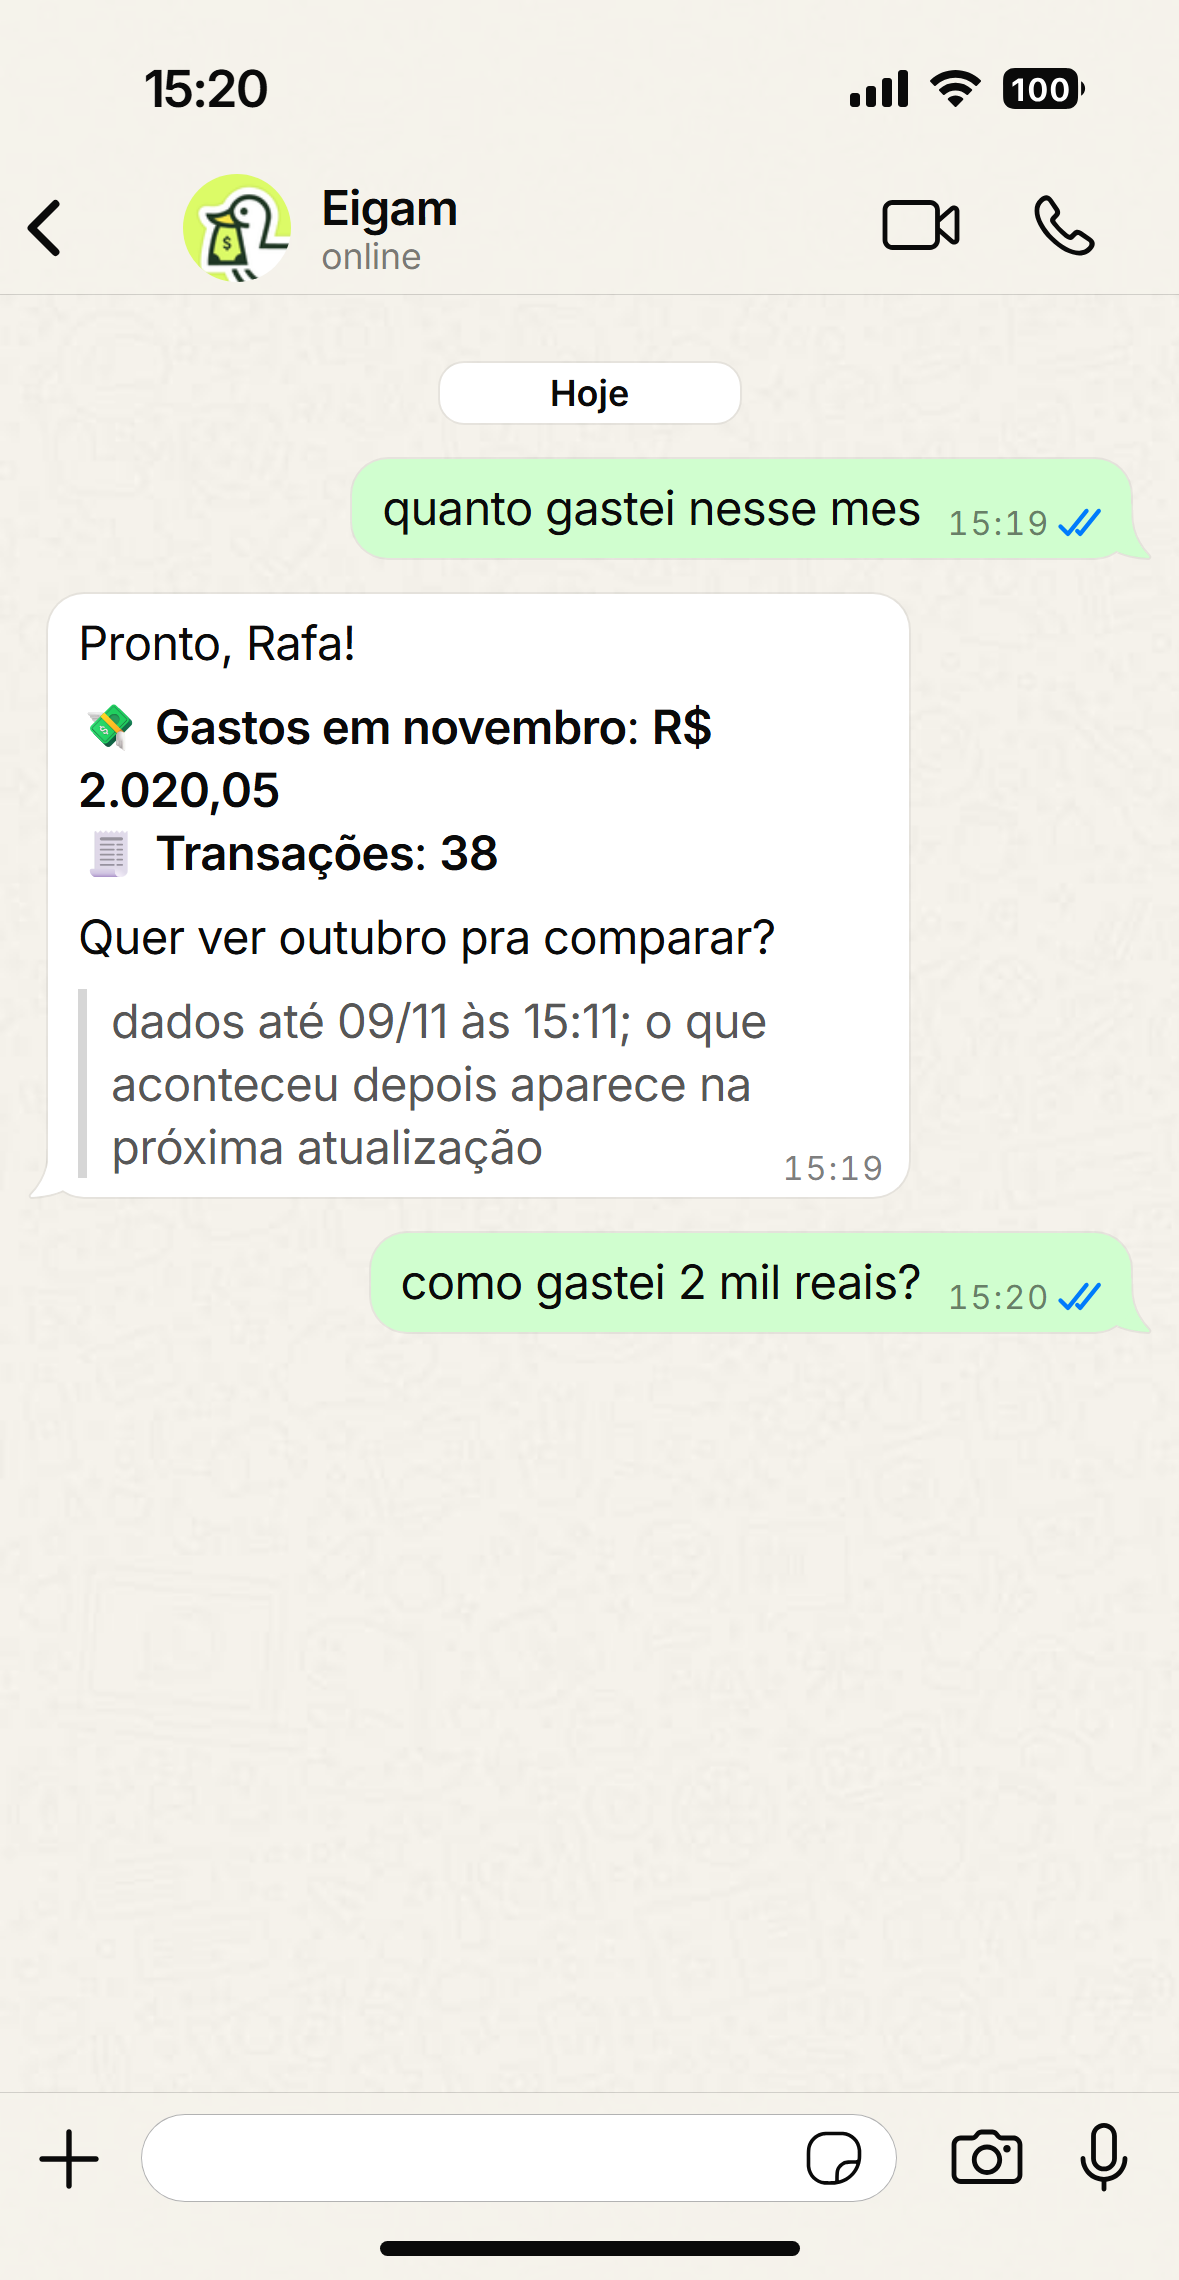
\includegraphics[width=\textwidth]{images/resultados/fluxos/fluxo_consulta_a.png}
    \end{minipage}\hfill
    \begin{minipage}[t]{0.32\textwidth}
        \centering
        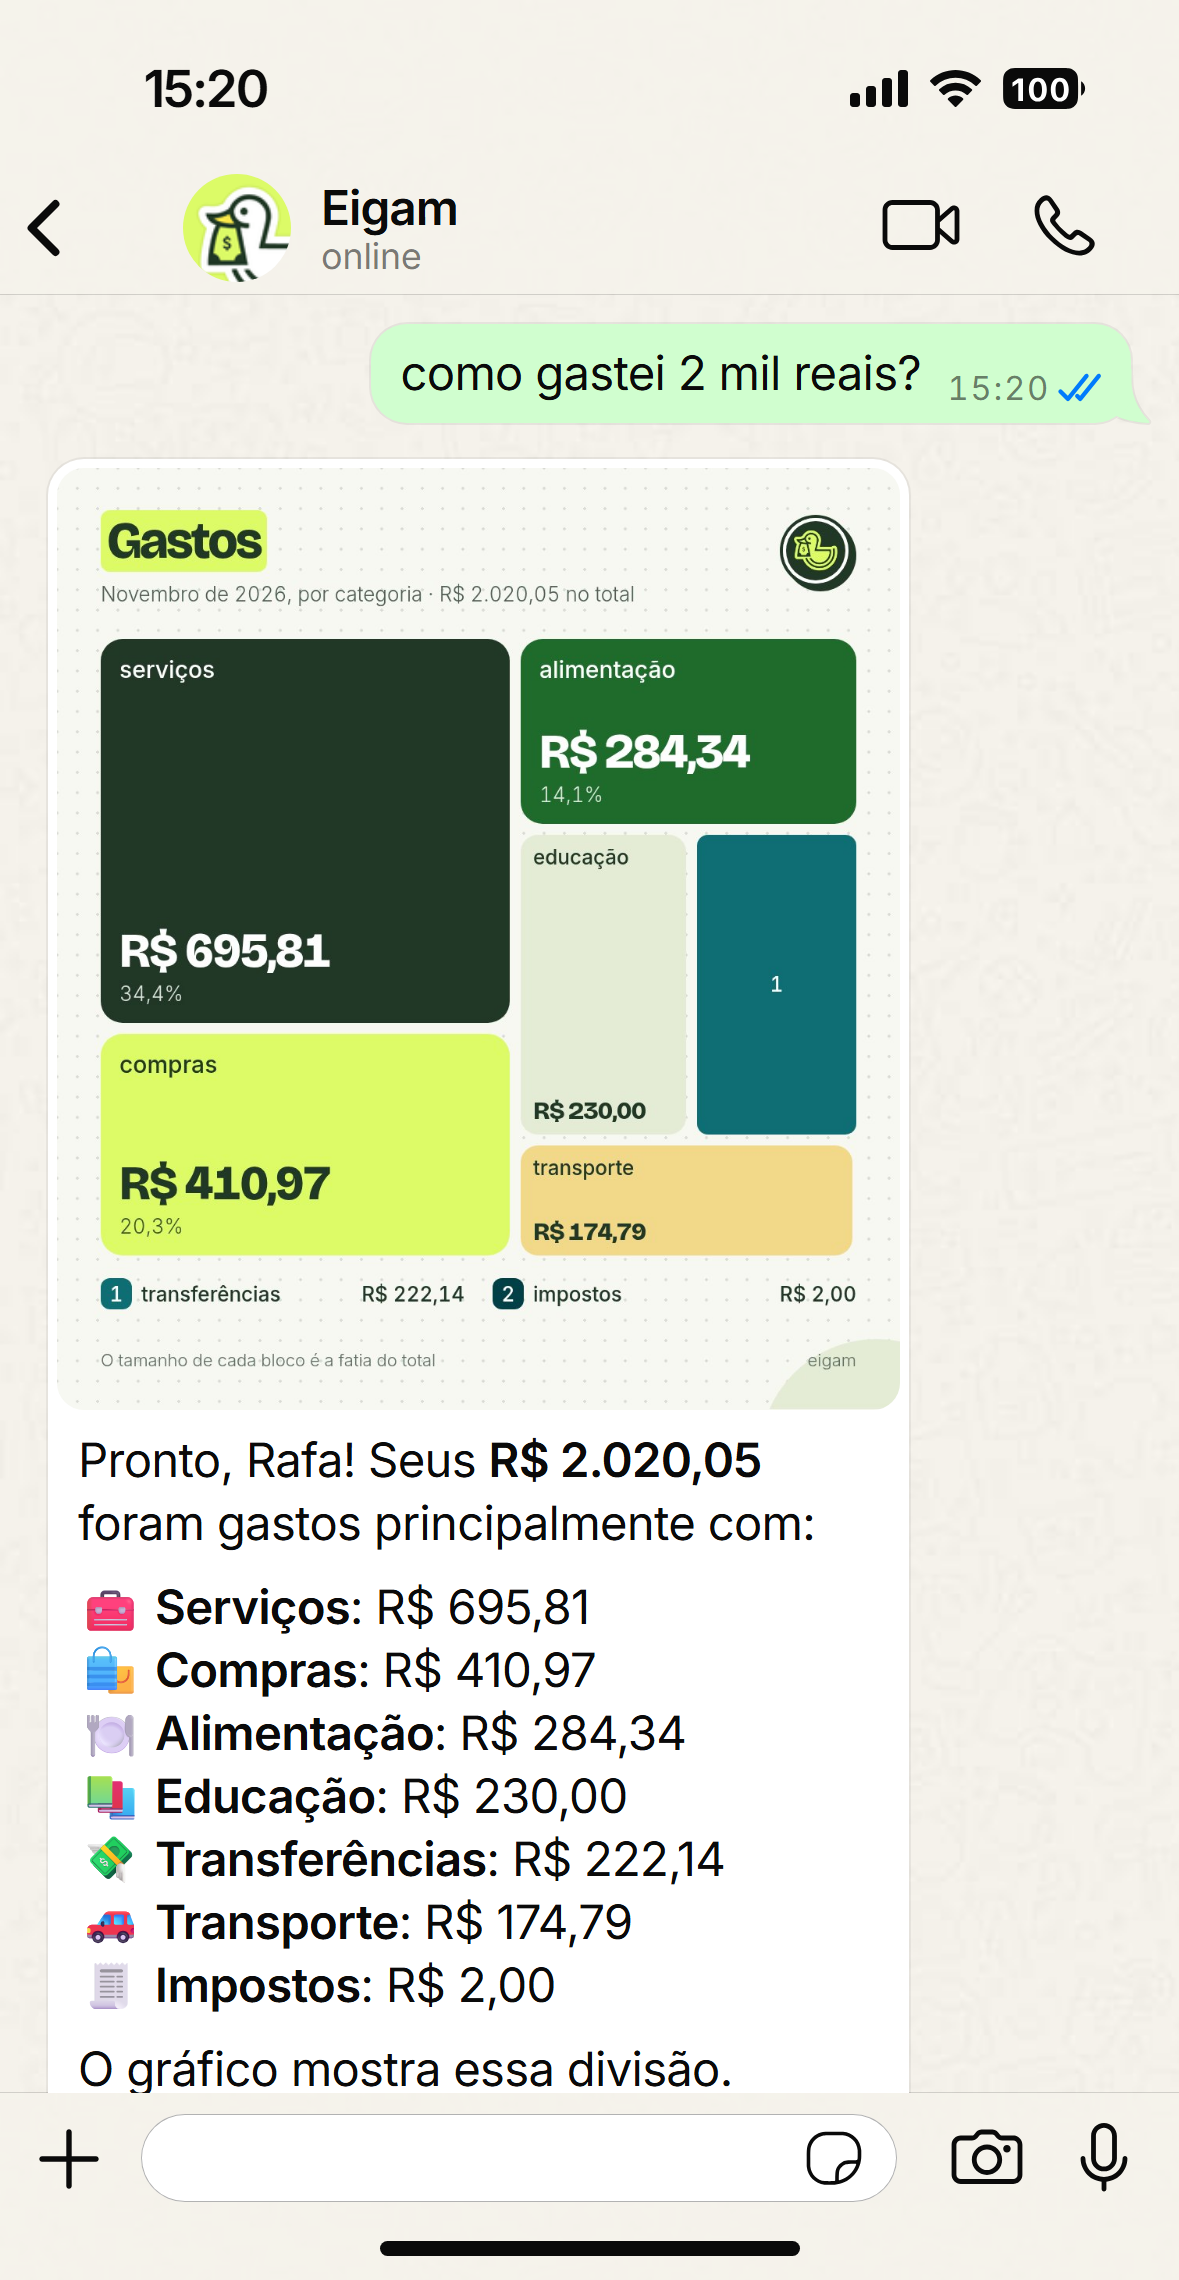
\includegraphics[width=\textwidth]{images/resultados/fluxos/fluxo_consulta_b.png}
    \end{minipage}\hfill
    \begin{minipage}[t]{0.32\textwidth}
        \centering
        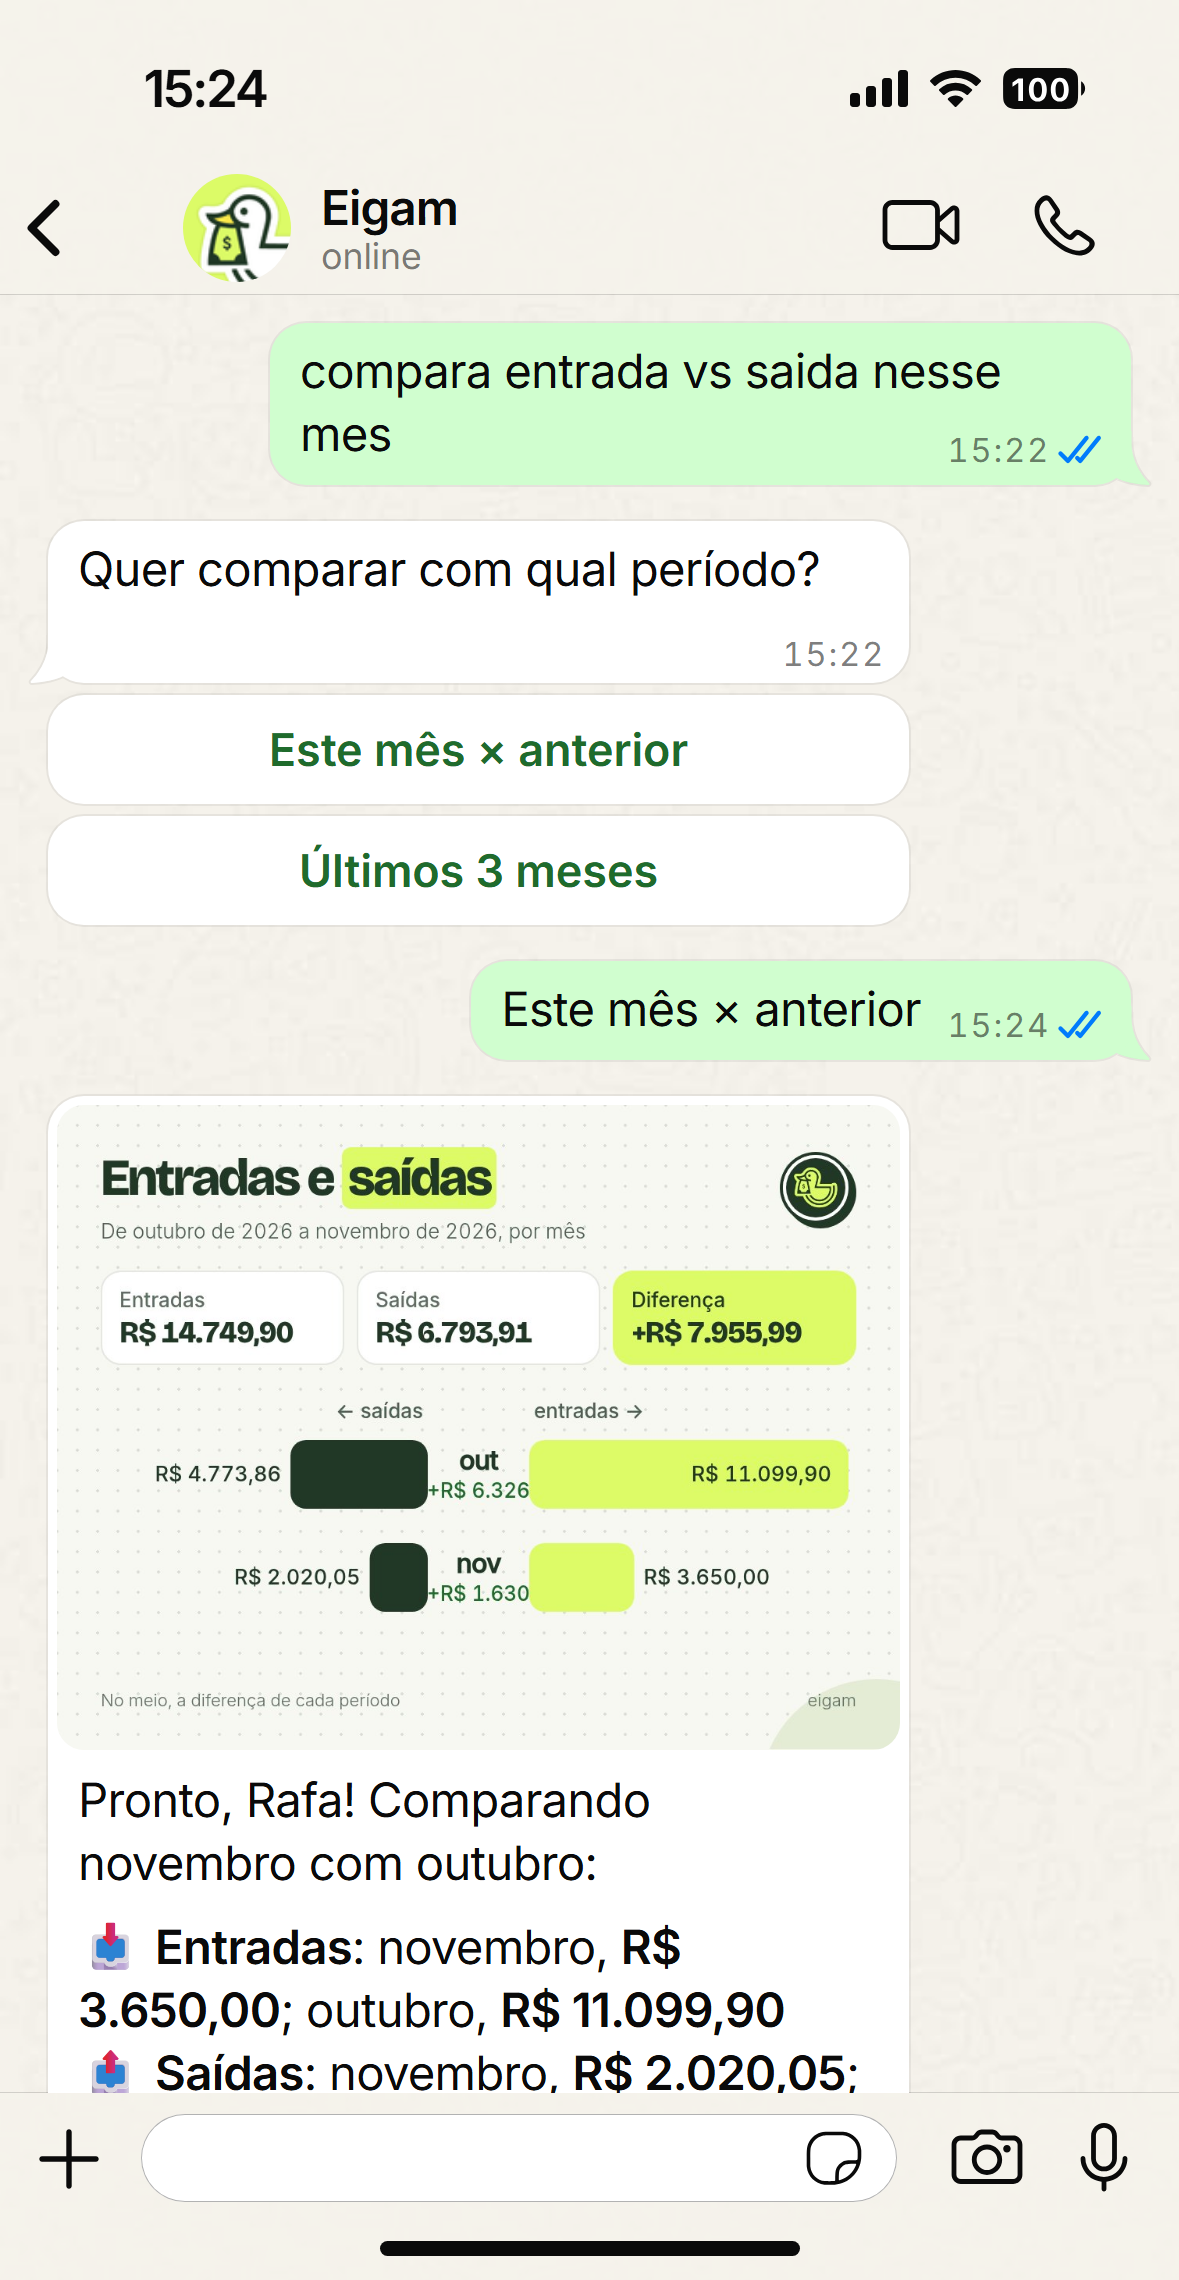
\includegraphics[width=\textwidth]{images/resultados/fluxos/fluxo_consulta_c.png}
    \end{minipage}
    \authorssource
\end{figure}

O fluxo do PIN (Figura~\ref{fig:fluxo_pin}) demonstra o mascaramento determinístico. Sem o token de privilégio, a pergunta sobre o gasto com roupas foi respondida apenas com o pedido do PIN; o PIN correto emitiu o token de oito horas, e a consulta pendente foi retomada na mesma mensagem, com o total do ano, a observação de que tudo foi pago no cartão de crédito, as parcelas de compras anteriores mantidas fora do total e o gráfico mensal. A decisão ocorre no publicador do servidor, depois dos \textit{guardrails}, e nunca depende do modelo.

\begin{figure}[H]
    \centering
    \caption{Fluxo de liberação de valores pelo PIN}
    \label{fig:fluxo_pin}
    \begin{minipage}[t]{0.32\textwidth}
        \centering
        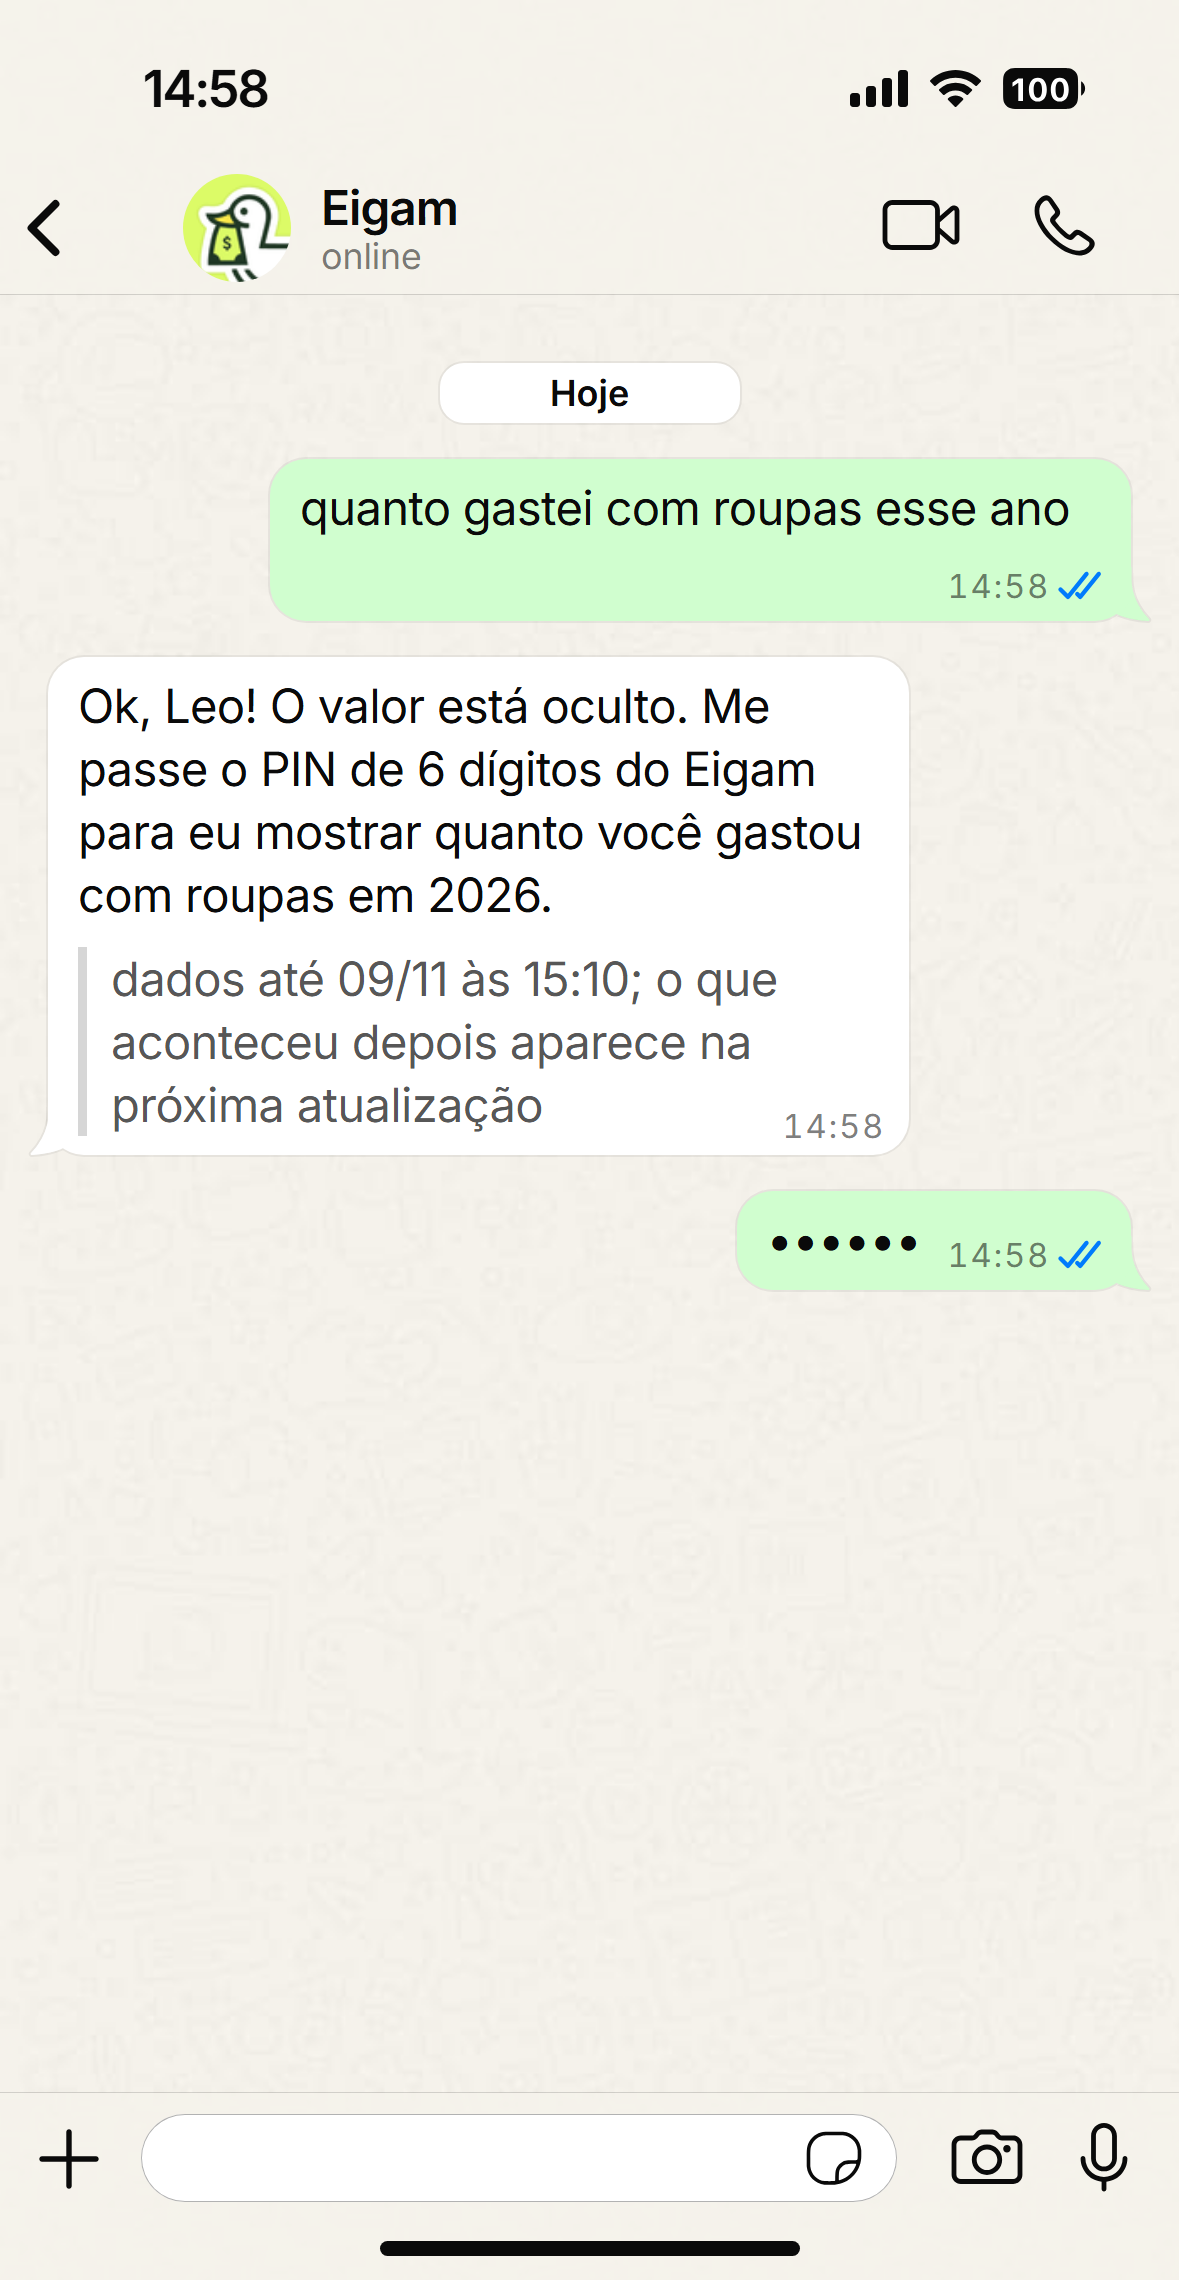
\includegraphics[width=\textwidth]{images/resultados/fluxos/fluxo_pin_a.png}
    \end{minipage}\hfill
    \begin{minipage}[t]{0.32\textwidth}
        \centering
        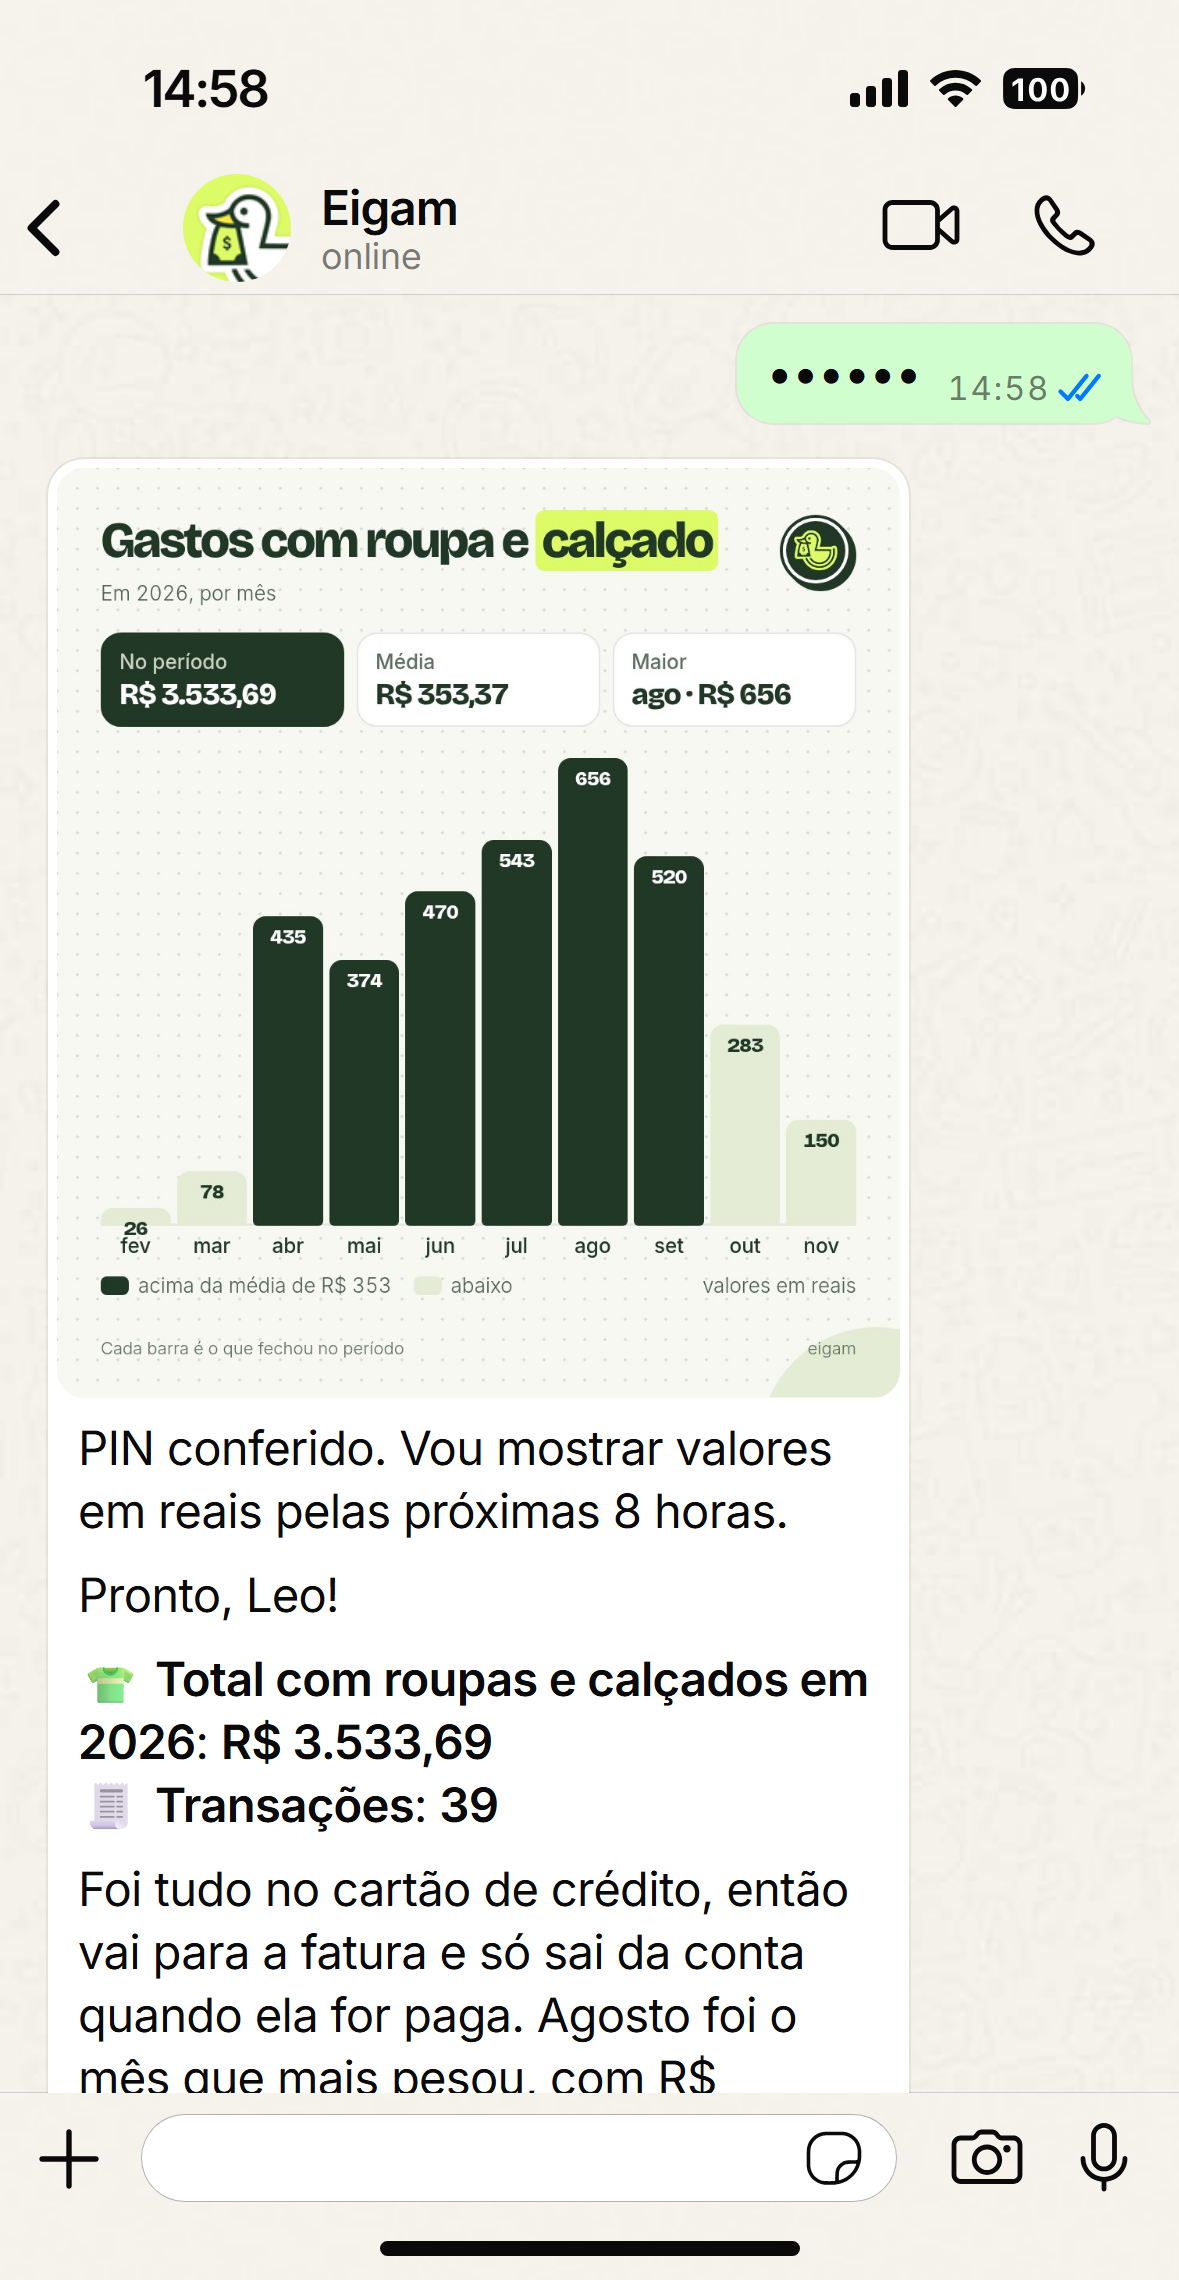
\includegraphics[width=\textwidth]{images/resultados/fluxos/fluxo_pin_b.png}
    \end{minipage}\hfill
    \begin{minipage}[t]{0.32\textwidth}
        \centering
        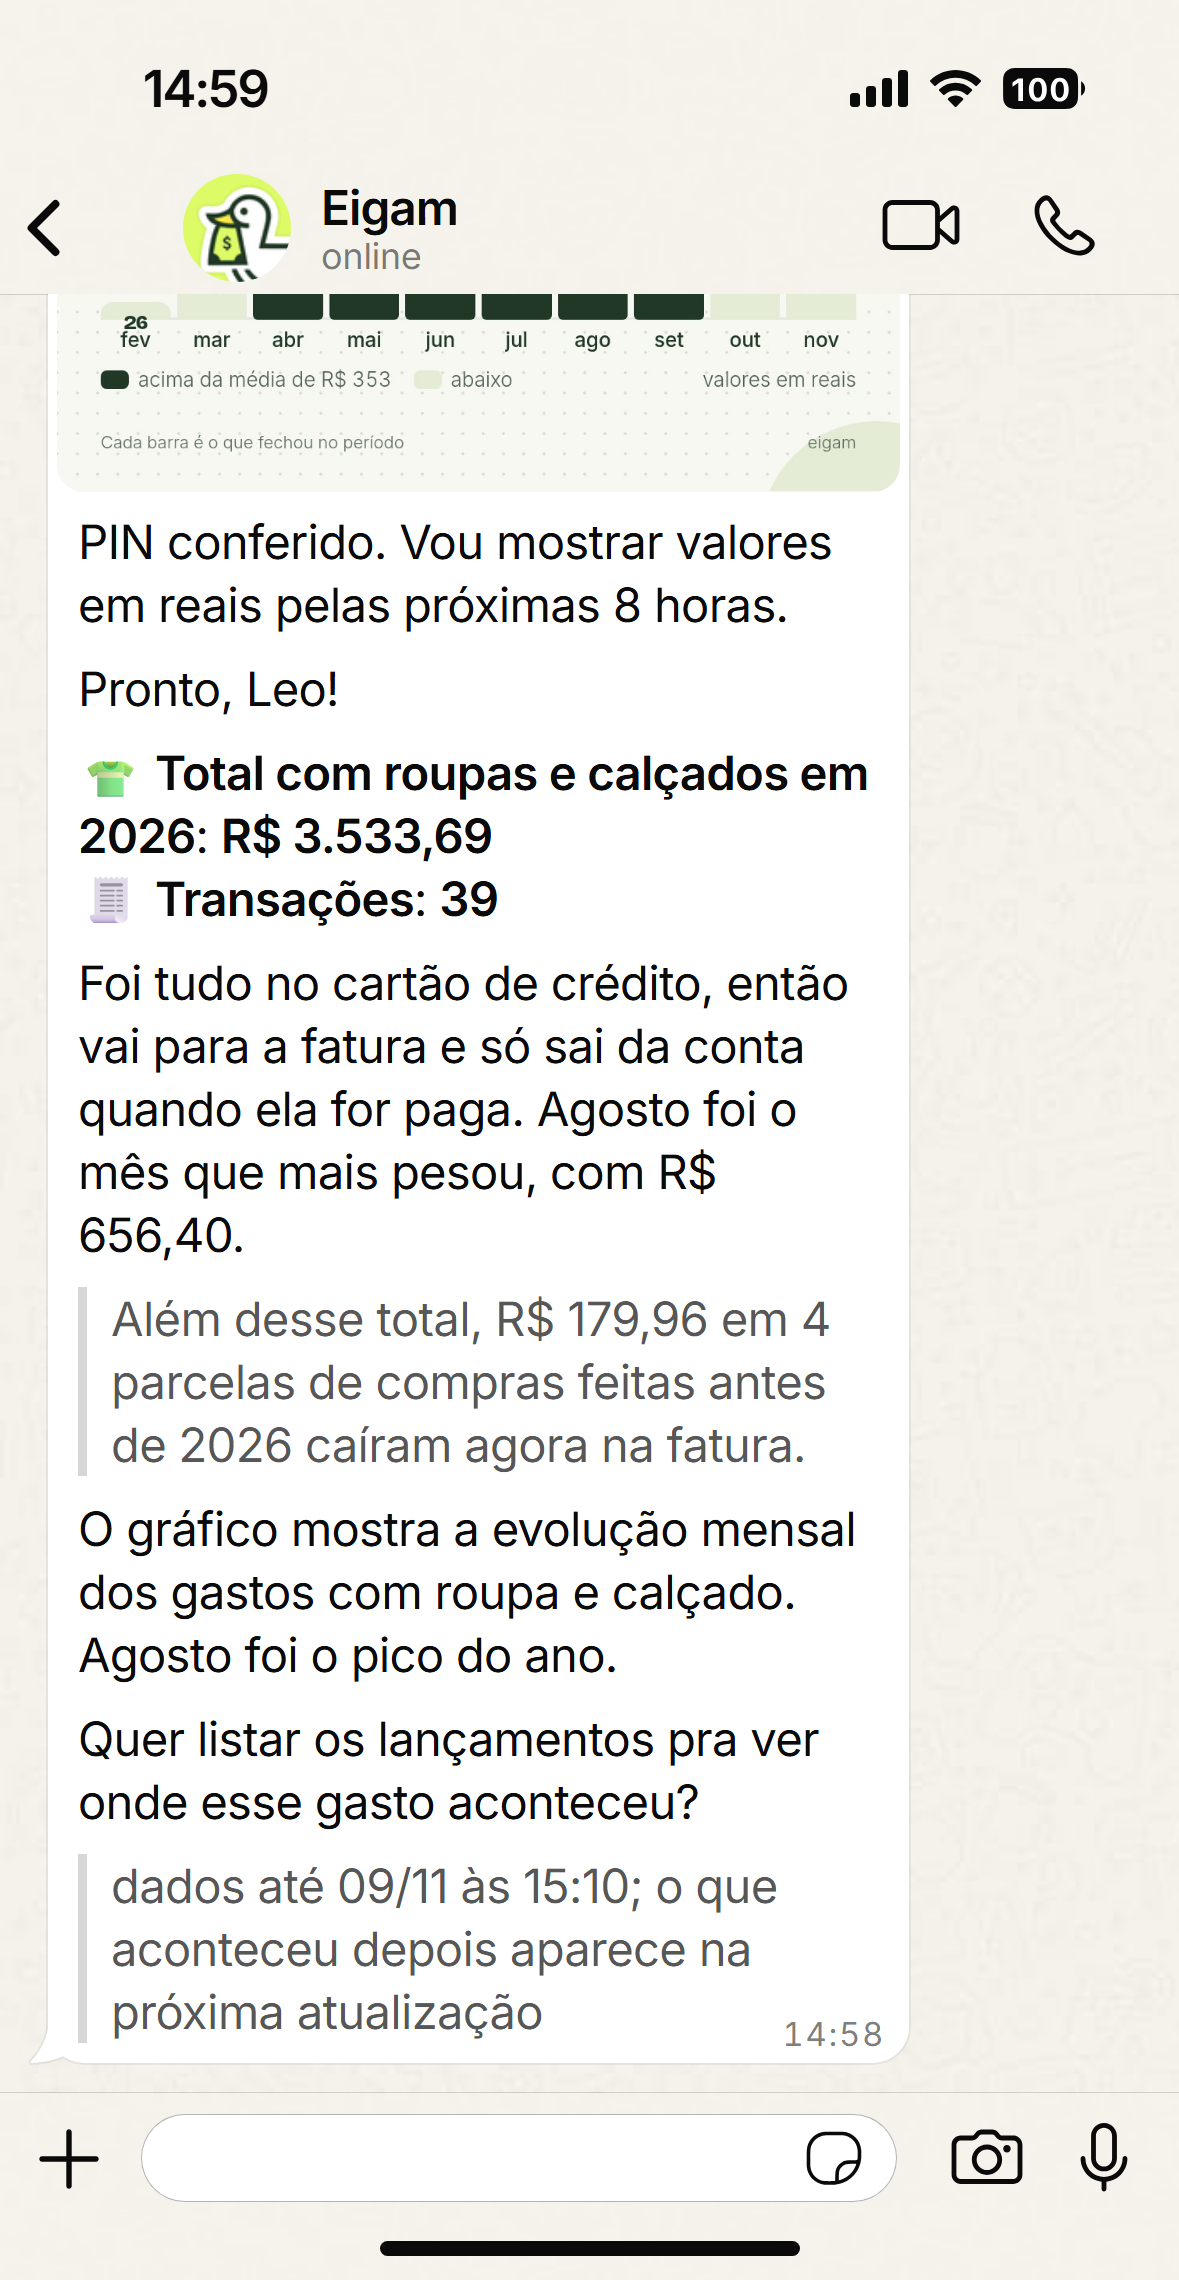
\includegraphics[width=\textwidth]{images/resultados/fluxos/fluxo_pin_c.png}
    \end{minipage}
    \authorssource
\end{figure}

As metas (Figura~\ref{fig:fluxo_meta}) foram criadas por botões ou por uma frase livre, lida por regras determinísticas que extraem valor, categoria e período. Antes de gravar, o sistema mostrou a meta com o gasto já acumulado no mês: na primeira tentativa, um teto de R\$~700,00 para o gasto total já estava em 102\%, e o titular reformulou o pedido em uma única frase, restringindo o teto à alimentação, que confirmou com 22\% utilizados. Nenhuma meta é gravada sem a confirmação explícita.

\begin{figure}[H]
    \centering
    \caption{Fluxo de criação de meta de gasto}
    \label{fig:fluxo_meta}
    \begin{minipage}[t]{0.32\textwidth}
        \centering
        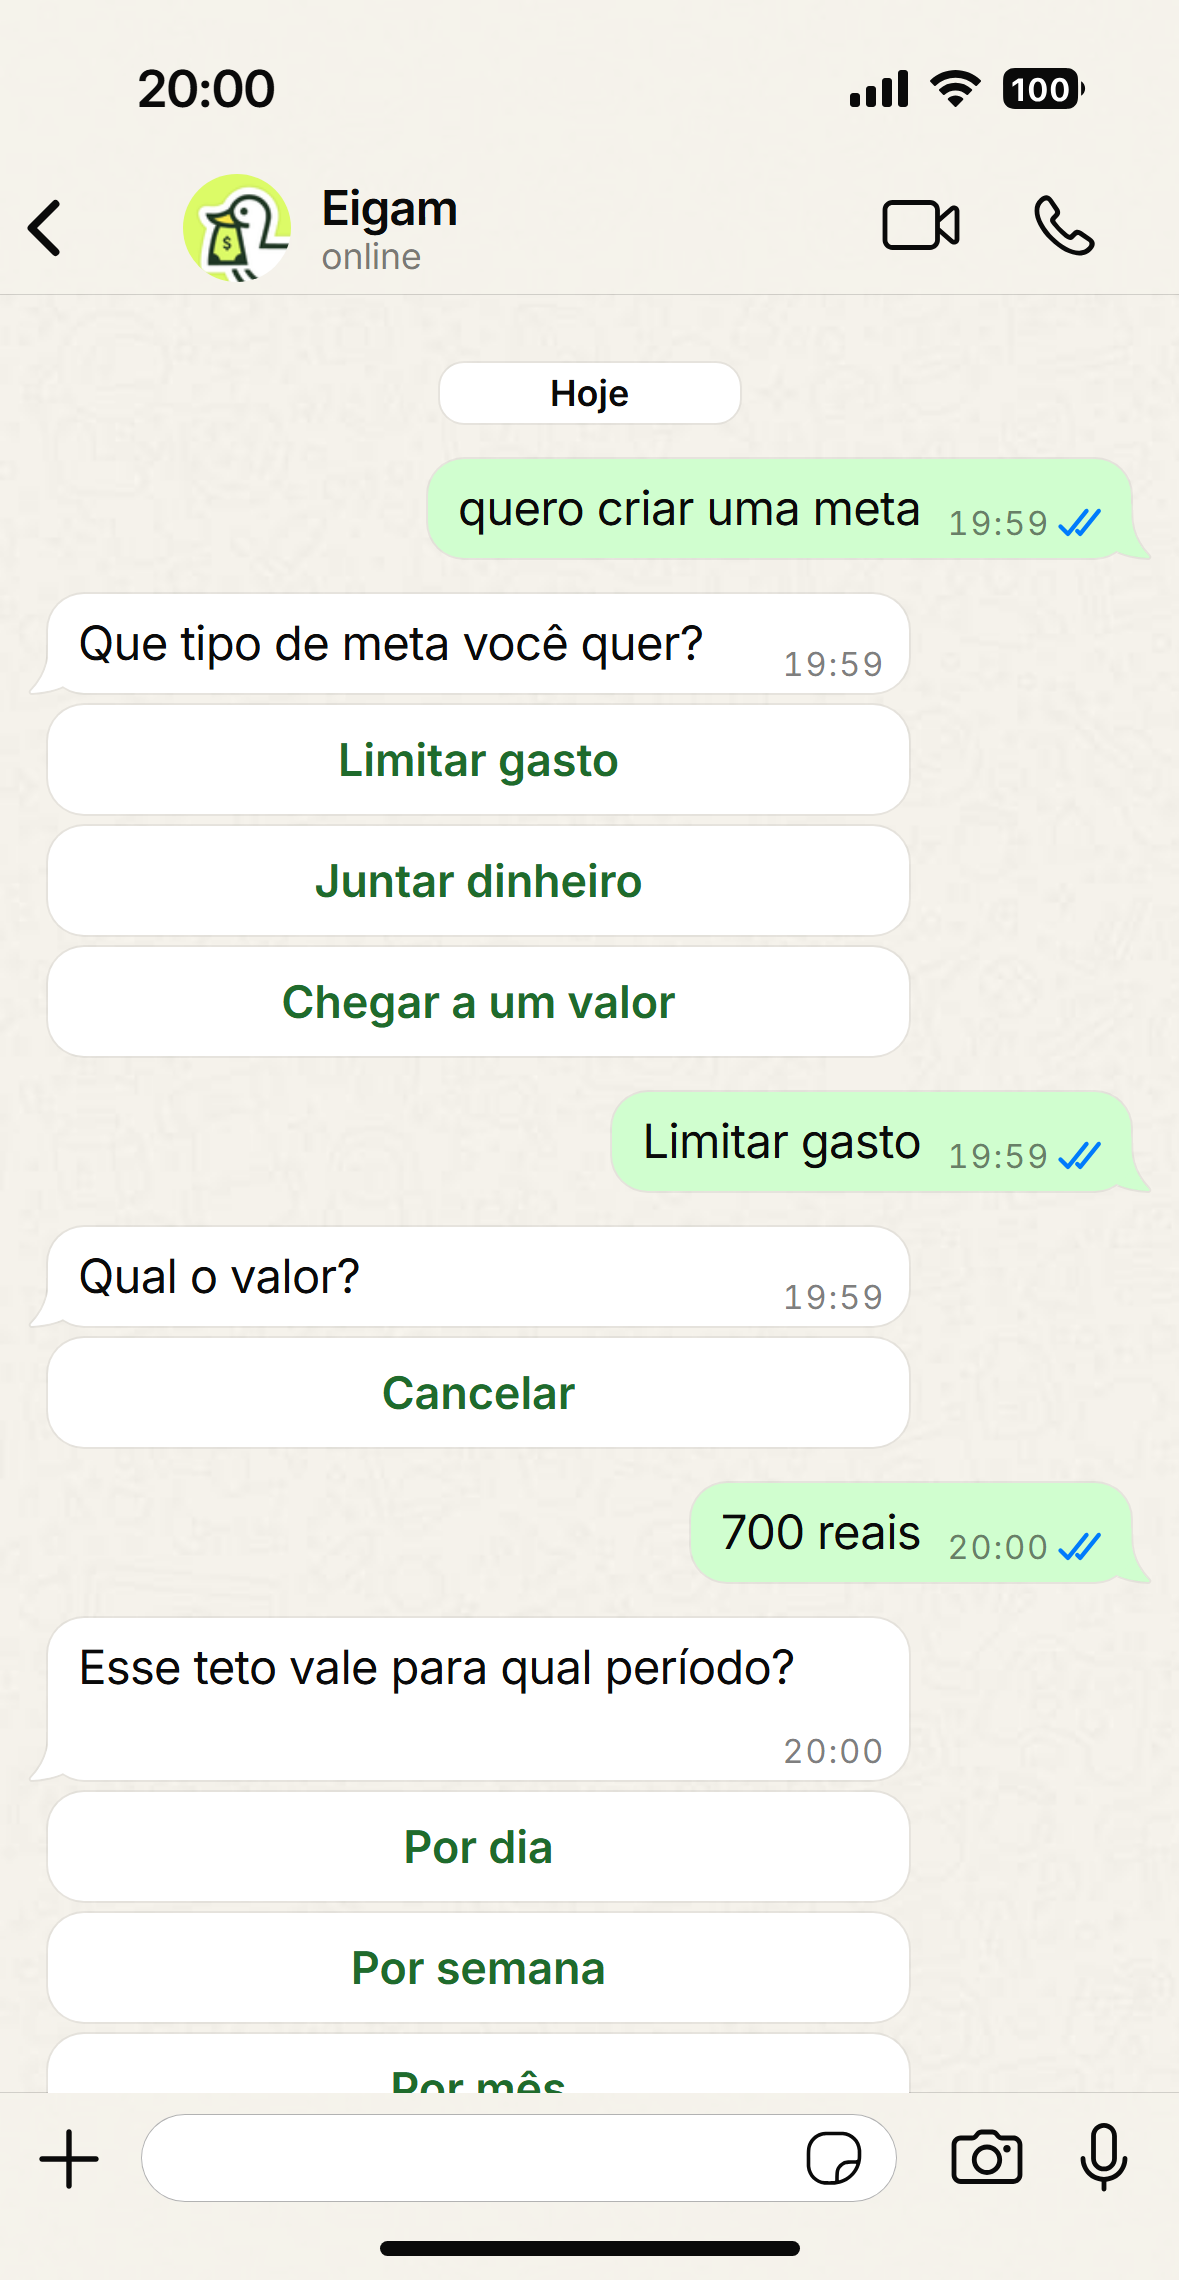
\includegraphics[width=\textwidth]{images/resultados/fluxos/fluxo_meta_a.png}
    \end{minipage}\hfill
    \begin{minipage}[t]{0.32\textwidth}
        \centering
        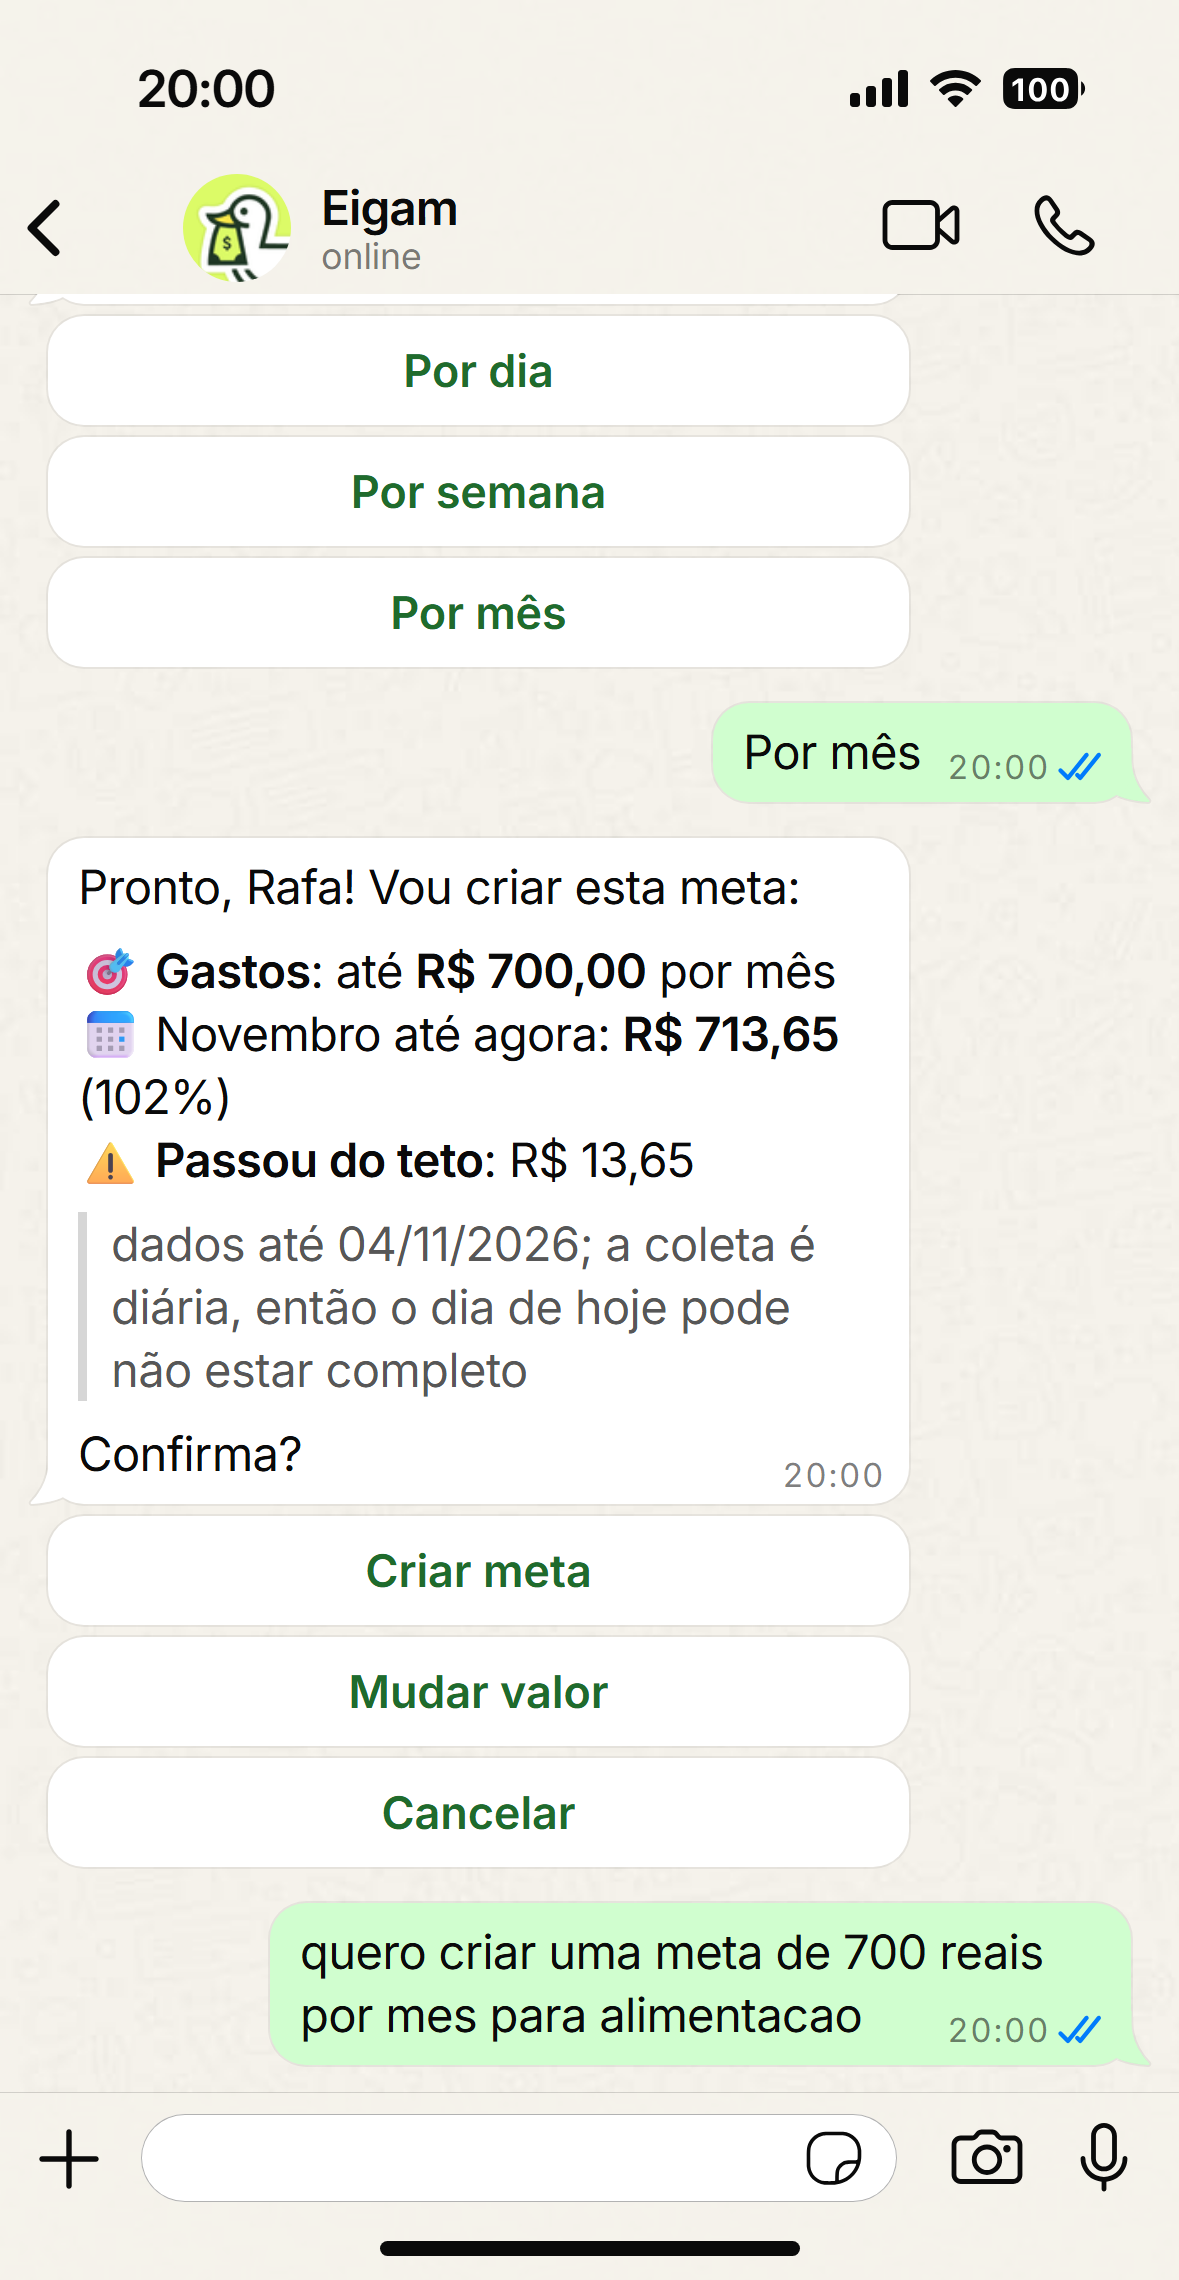
\includegraphics[width=\textwidth]{images/resultados/fluxos/fluxo_meta_b.png}
    \end{minipage}\hfill
    \begin{minipage}[t]{0.32\textwidth}
        \centering
        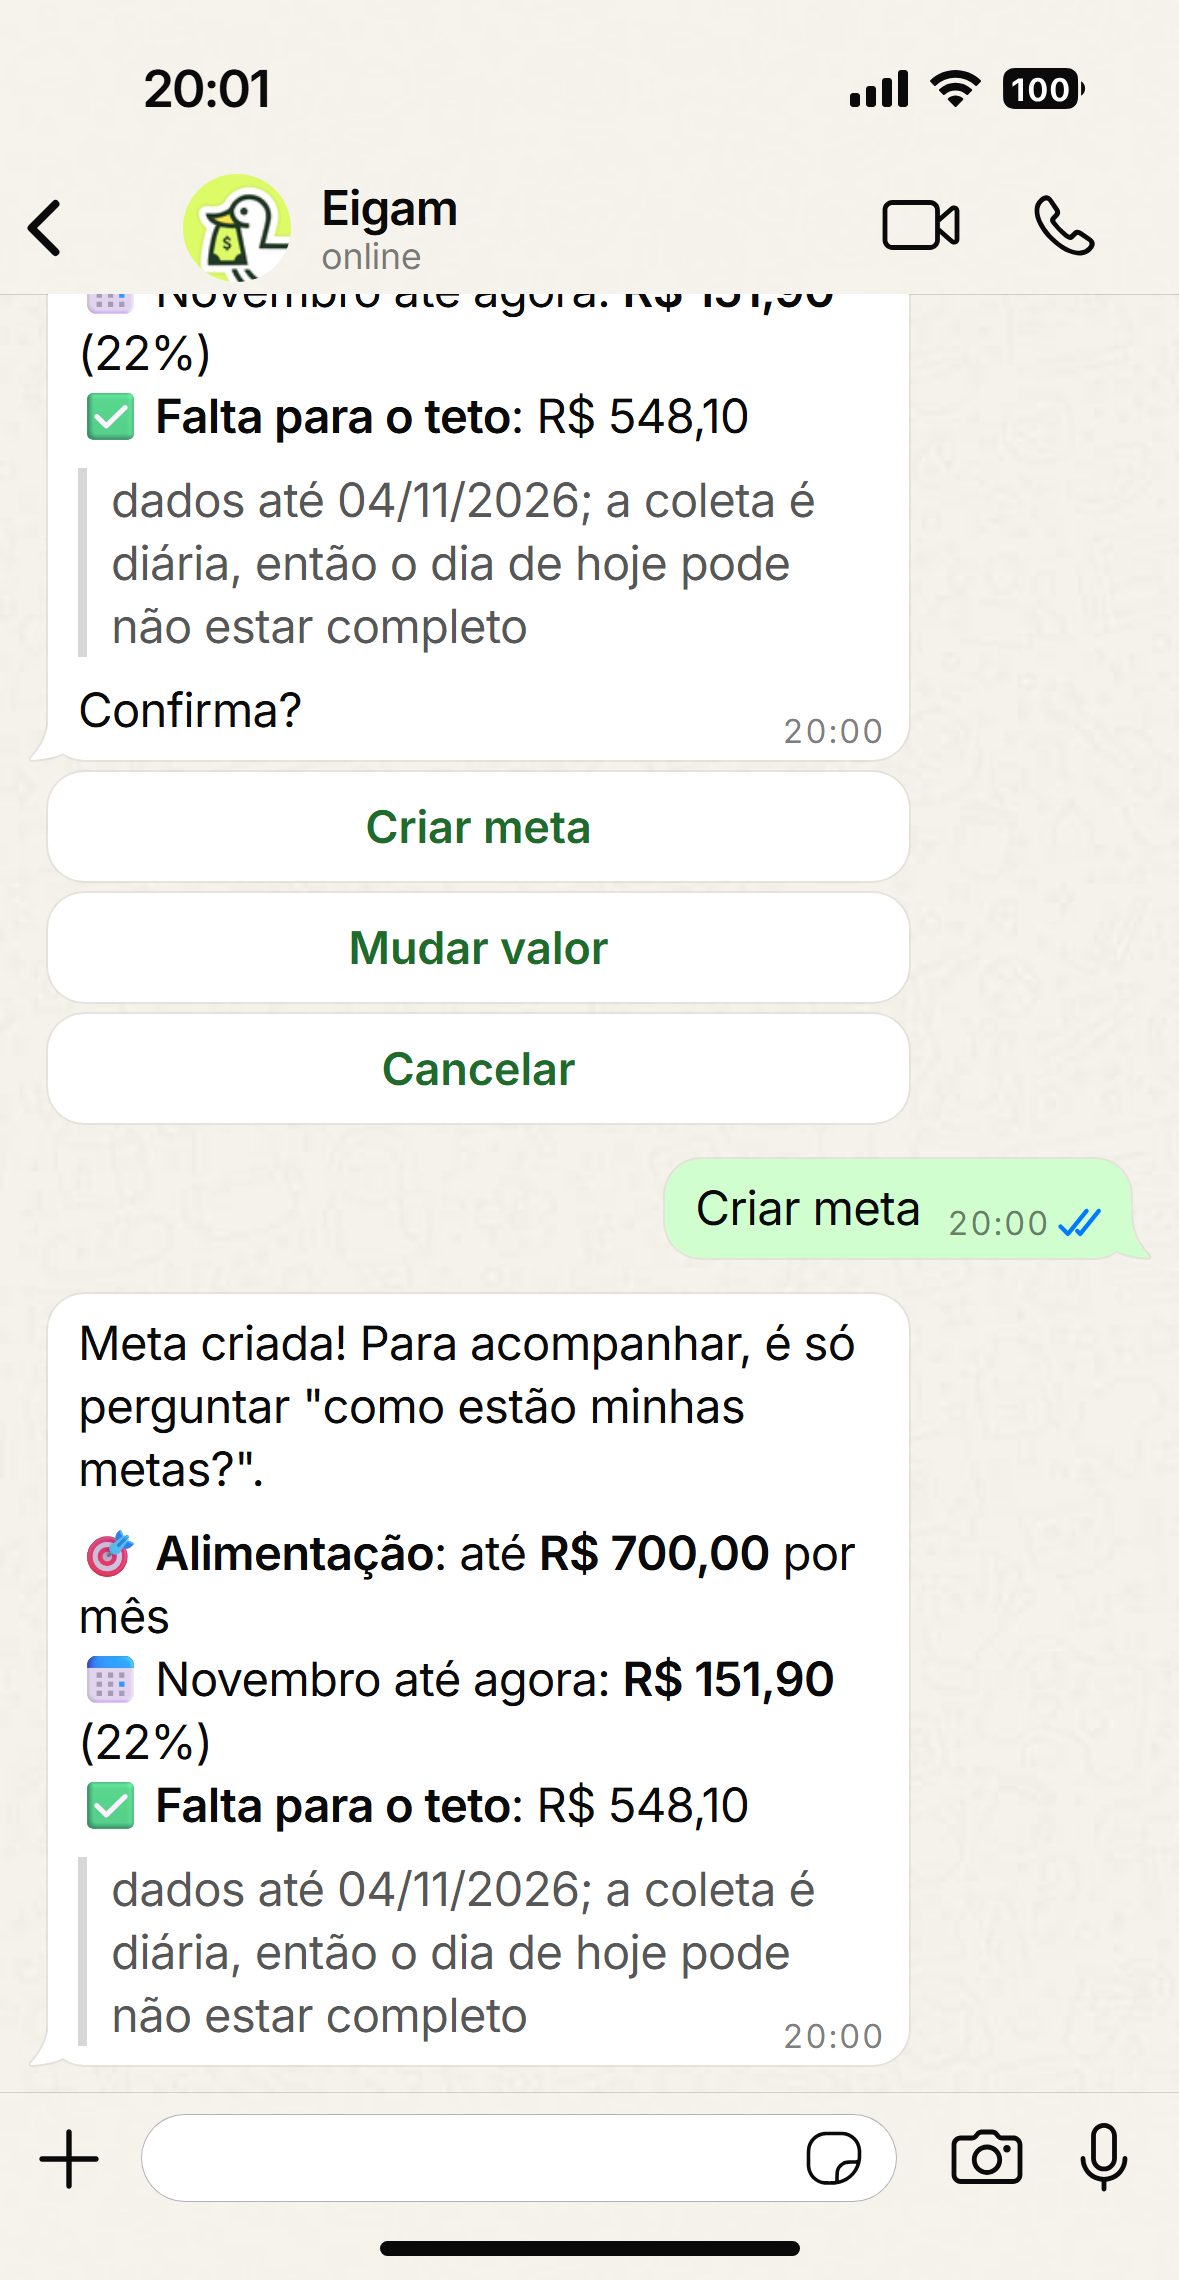
\includegraphics[width=\textwidth]{images/resultados/fluxos/fluxo_meta_c.png}
    \end{minipage}
    \authorssource
\end{figure}

As mensagens proativas seguem a mesma regra de privacidade (Figura~\ref{fig:fluxo_resumo}). No dia em que o titular liberou os valores com o PIN, o resumo semanal chegou por um modelo de mensagem aprovado no canal, com uma prévia que informa apenas a tendência do gasto em relação à semana anterior e a categoria que mais pesou, sem valor em reais, e com um botão para os detalhes. Ao tocar no botão, o titular recebeu o resumo completo em PDF, gerado no momento do pedido. Os avisos de metas e de movimentação usam o mesmo desenho de prévia sem valores, mas não haviam sido liberados no canal real durante o beta, conforme as limitações apresentadas adiante.

\begin{figure}[H]
    \centering
    \caption{Resumo semanal proativo, sem valores na prévia}
    \label{fig:fluxo_resumo}
    \begin{minipage}[t]{0.32\textwidth}
        \centering
        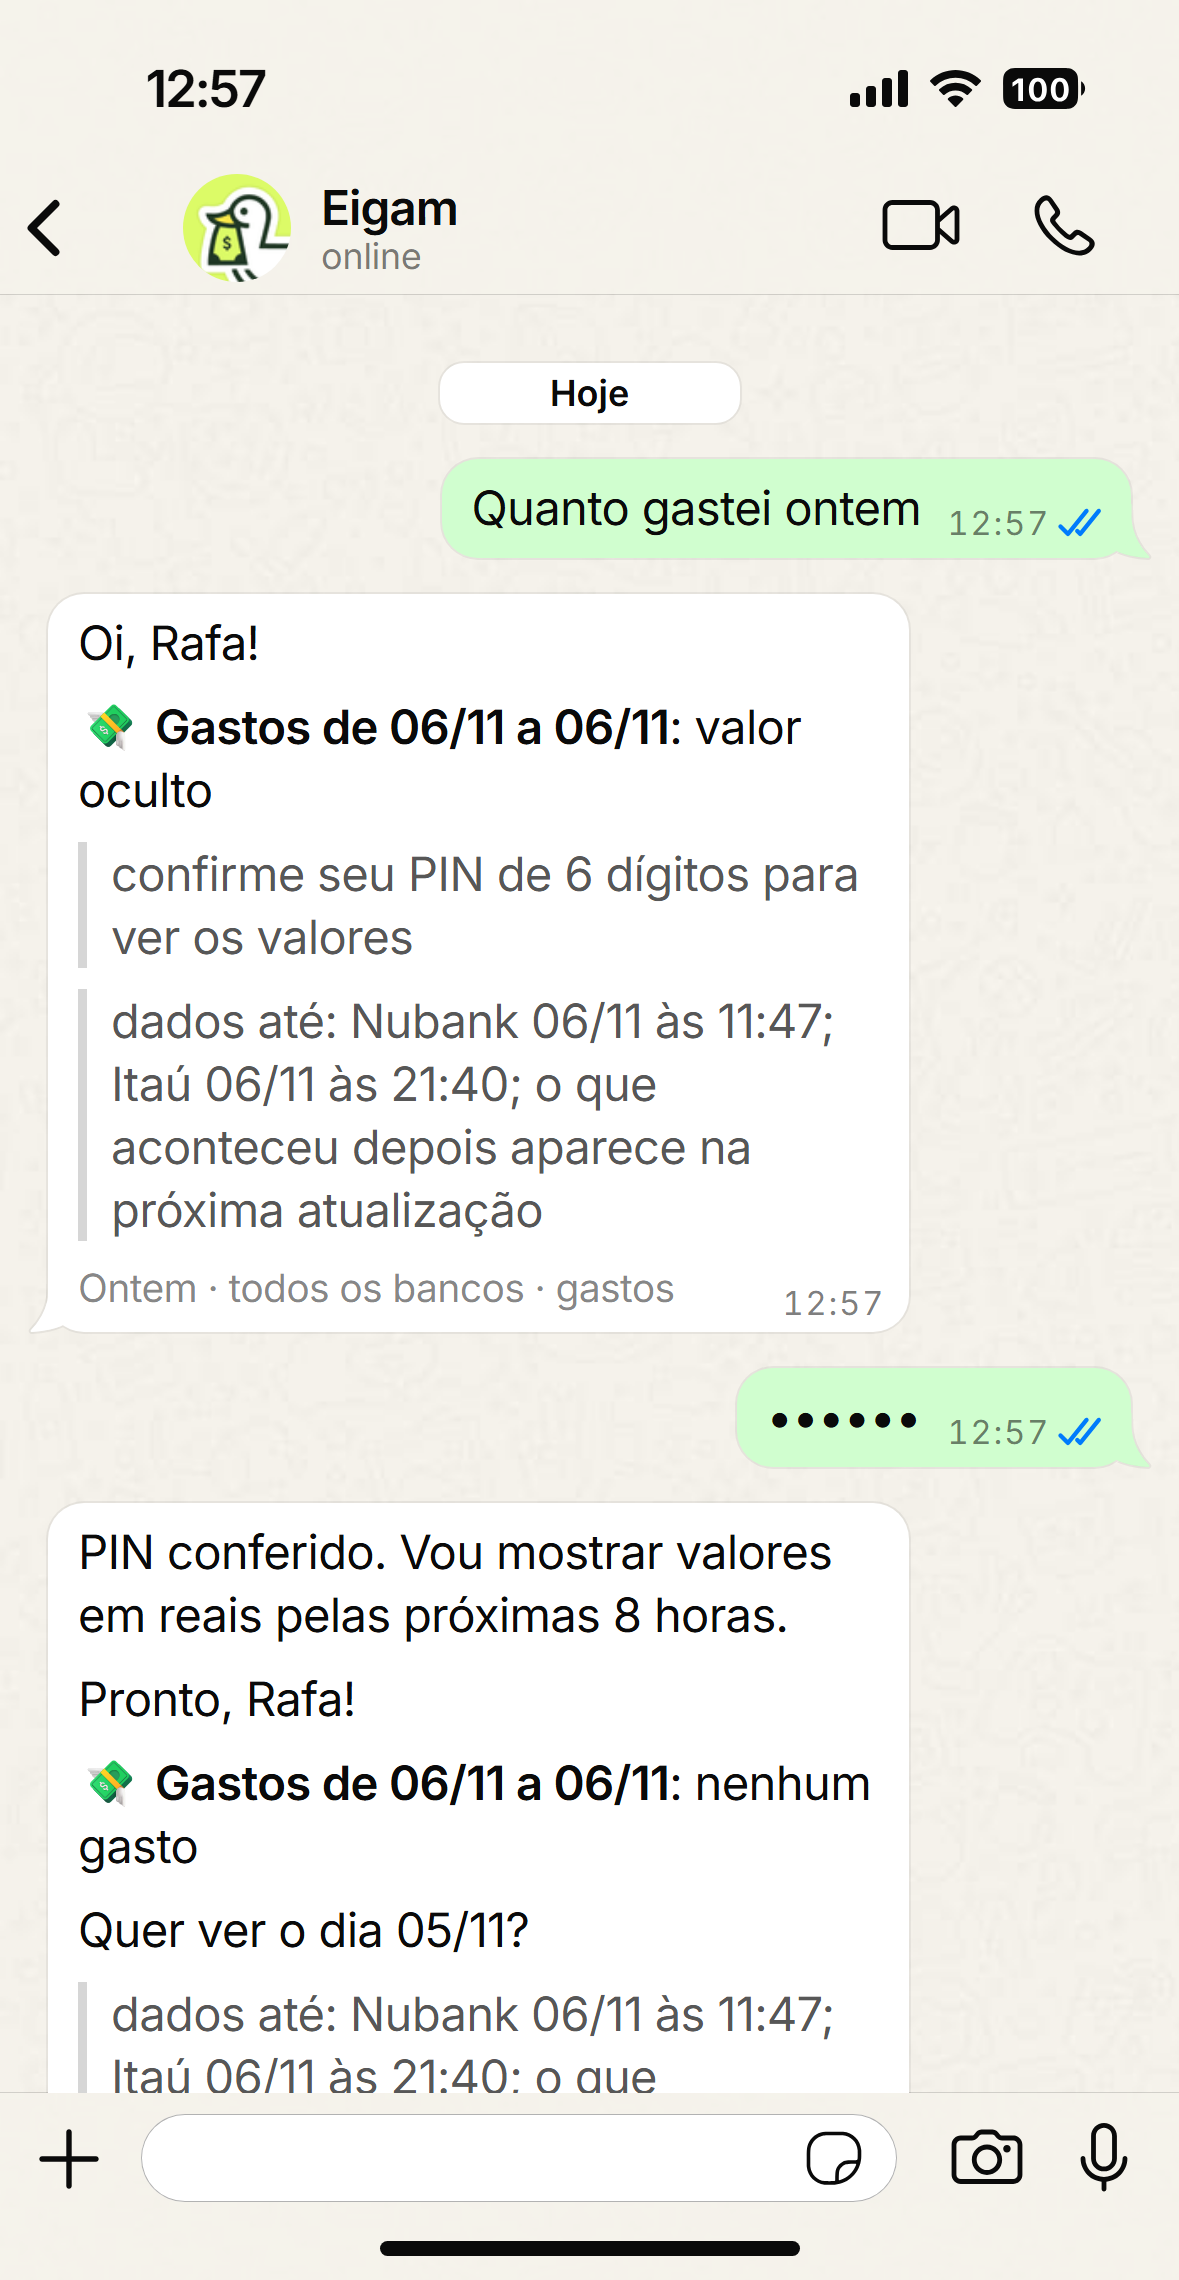
\includegraphics[width=\textwidth]{images/resultados/fluxos/fluxo_resumo_a.png}
    \end{minipage}\hfill
    \begin{minipage}[t]{0.32\textwidth}
        \centering
        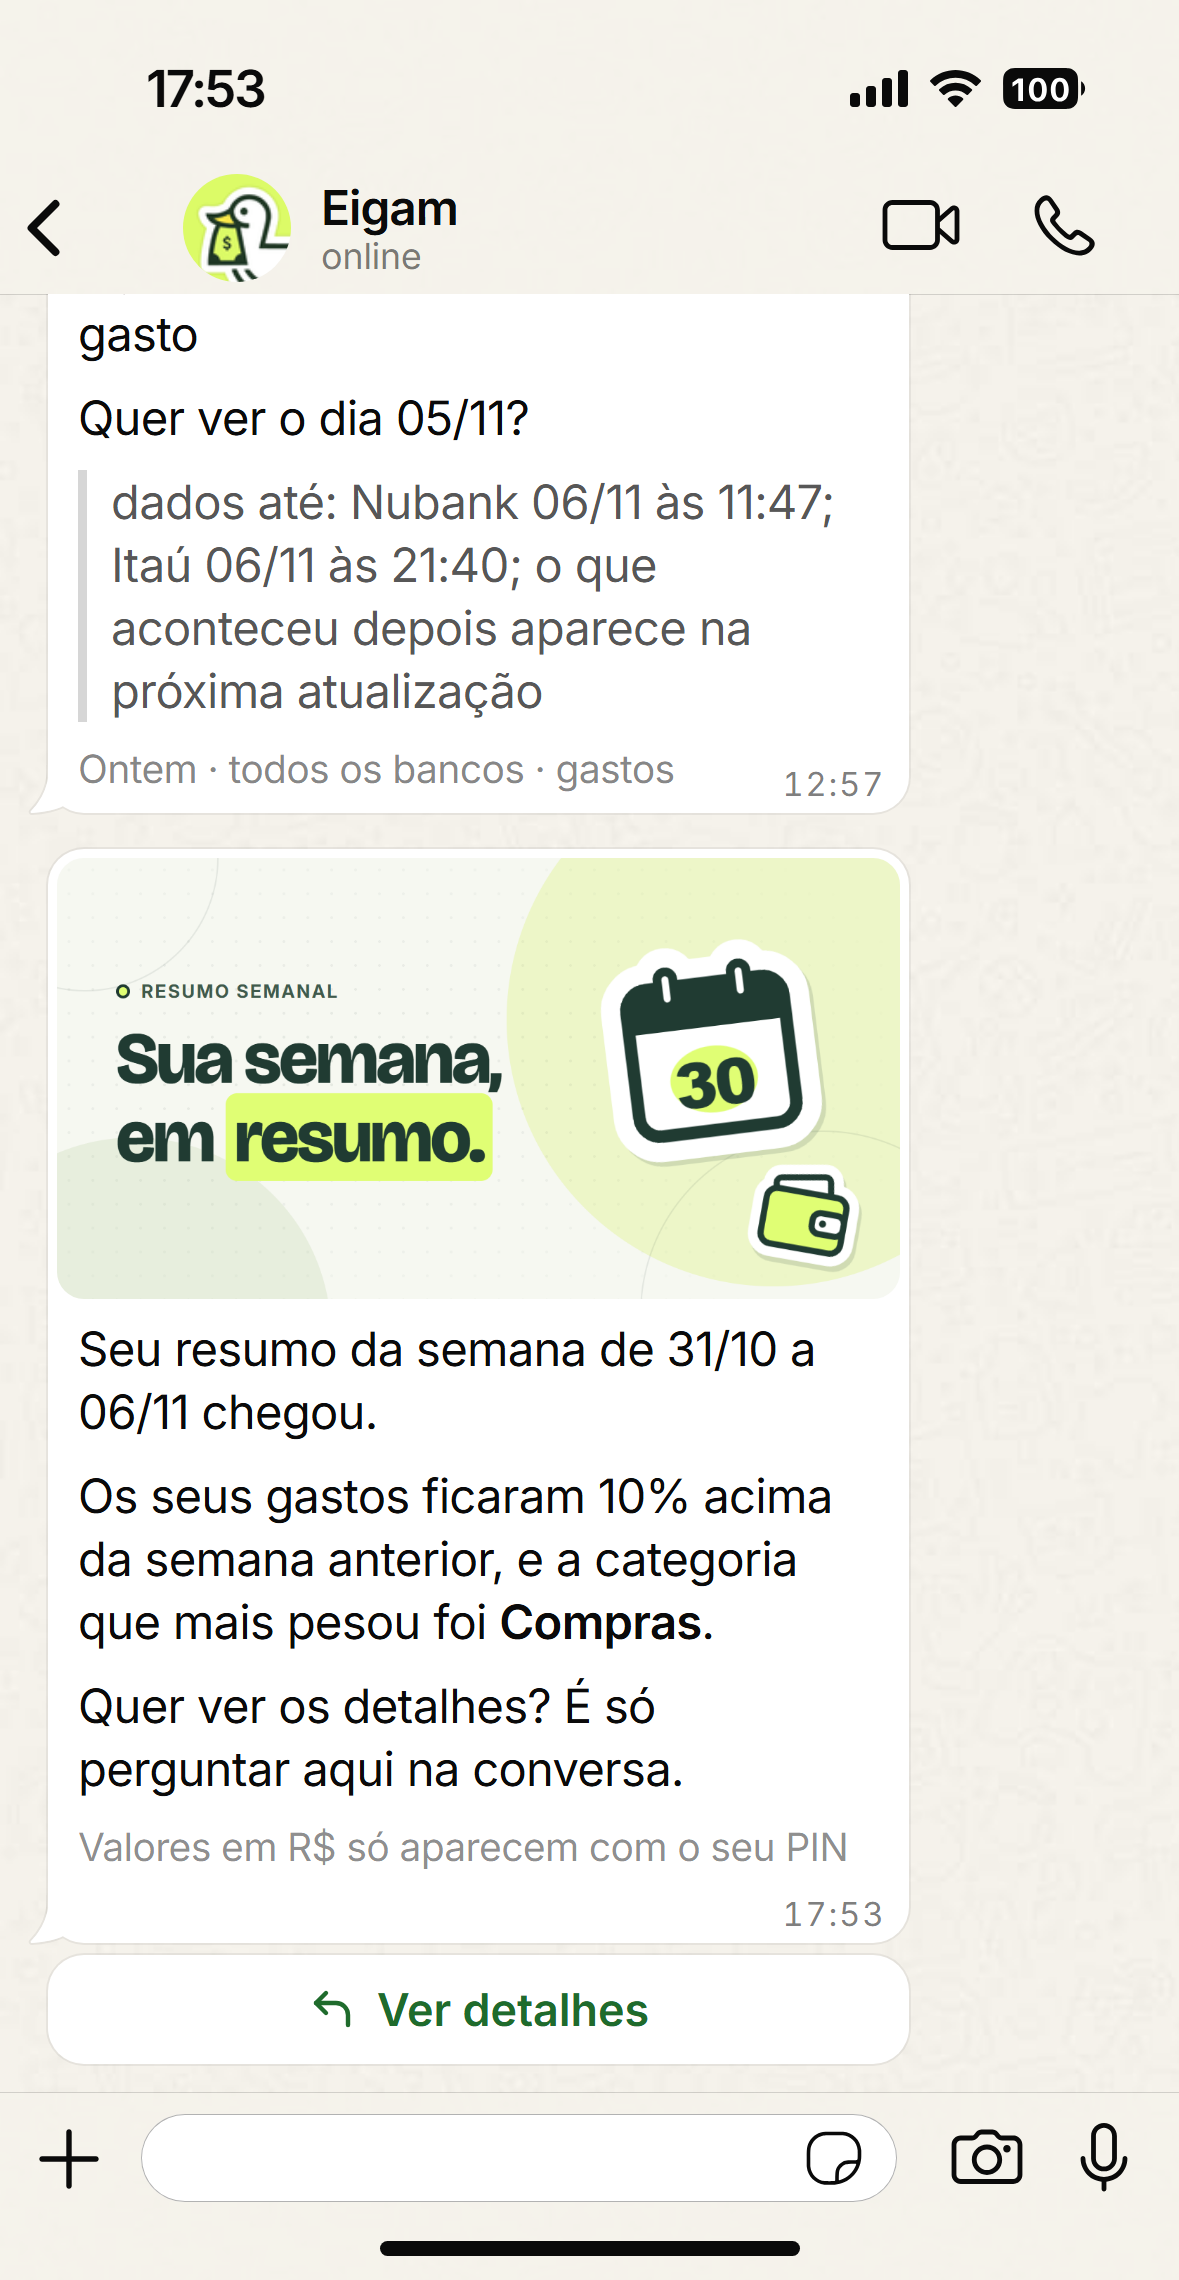
\includegraphics[width=\textwidth]{images/resultados/fluxos/fluxo_resumo_b.png}
    \end{minipage}\hfill
    \begin{minipage}[t]{0.32\textwidth}
        \centering
        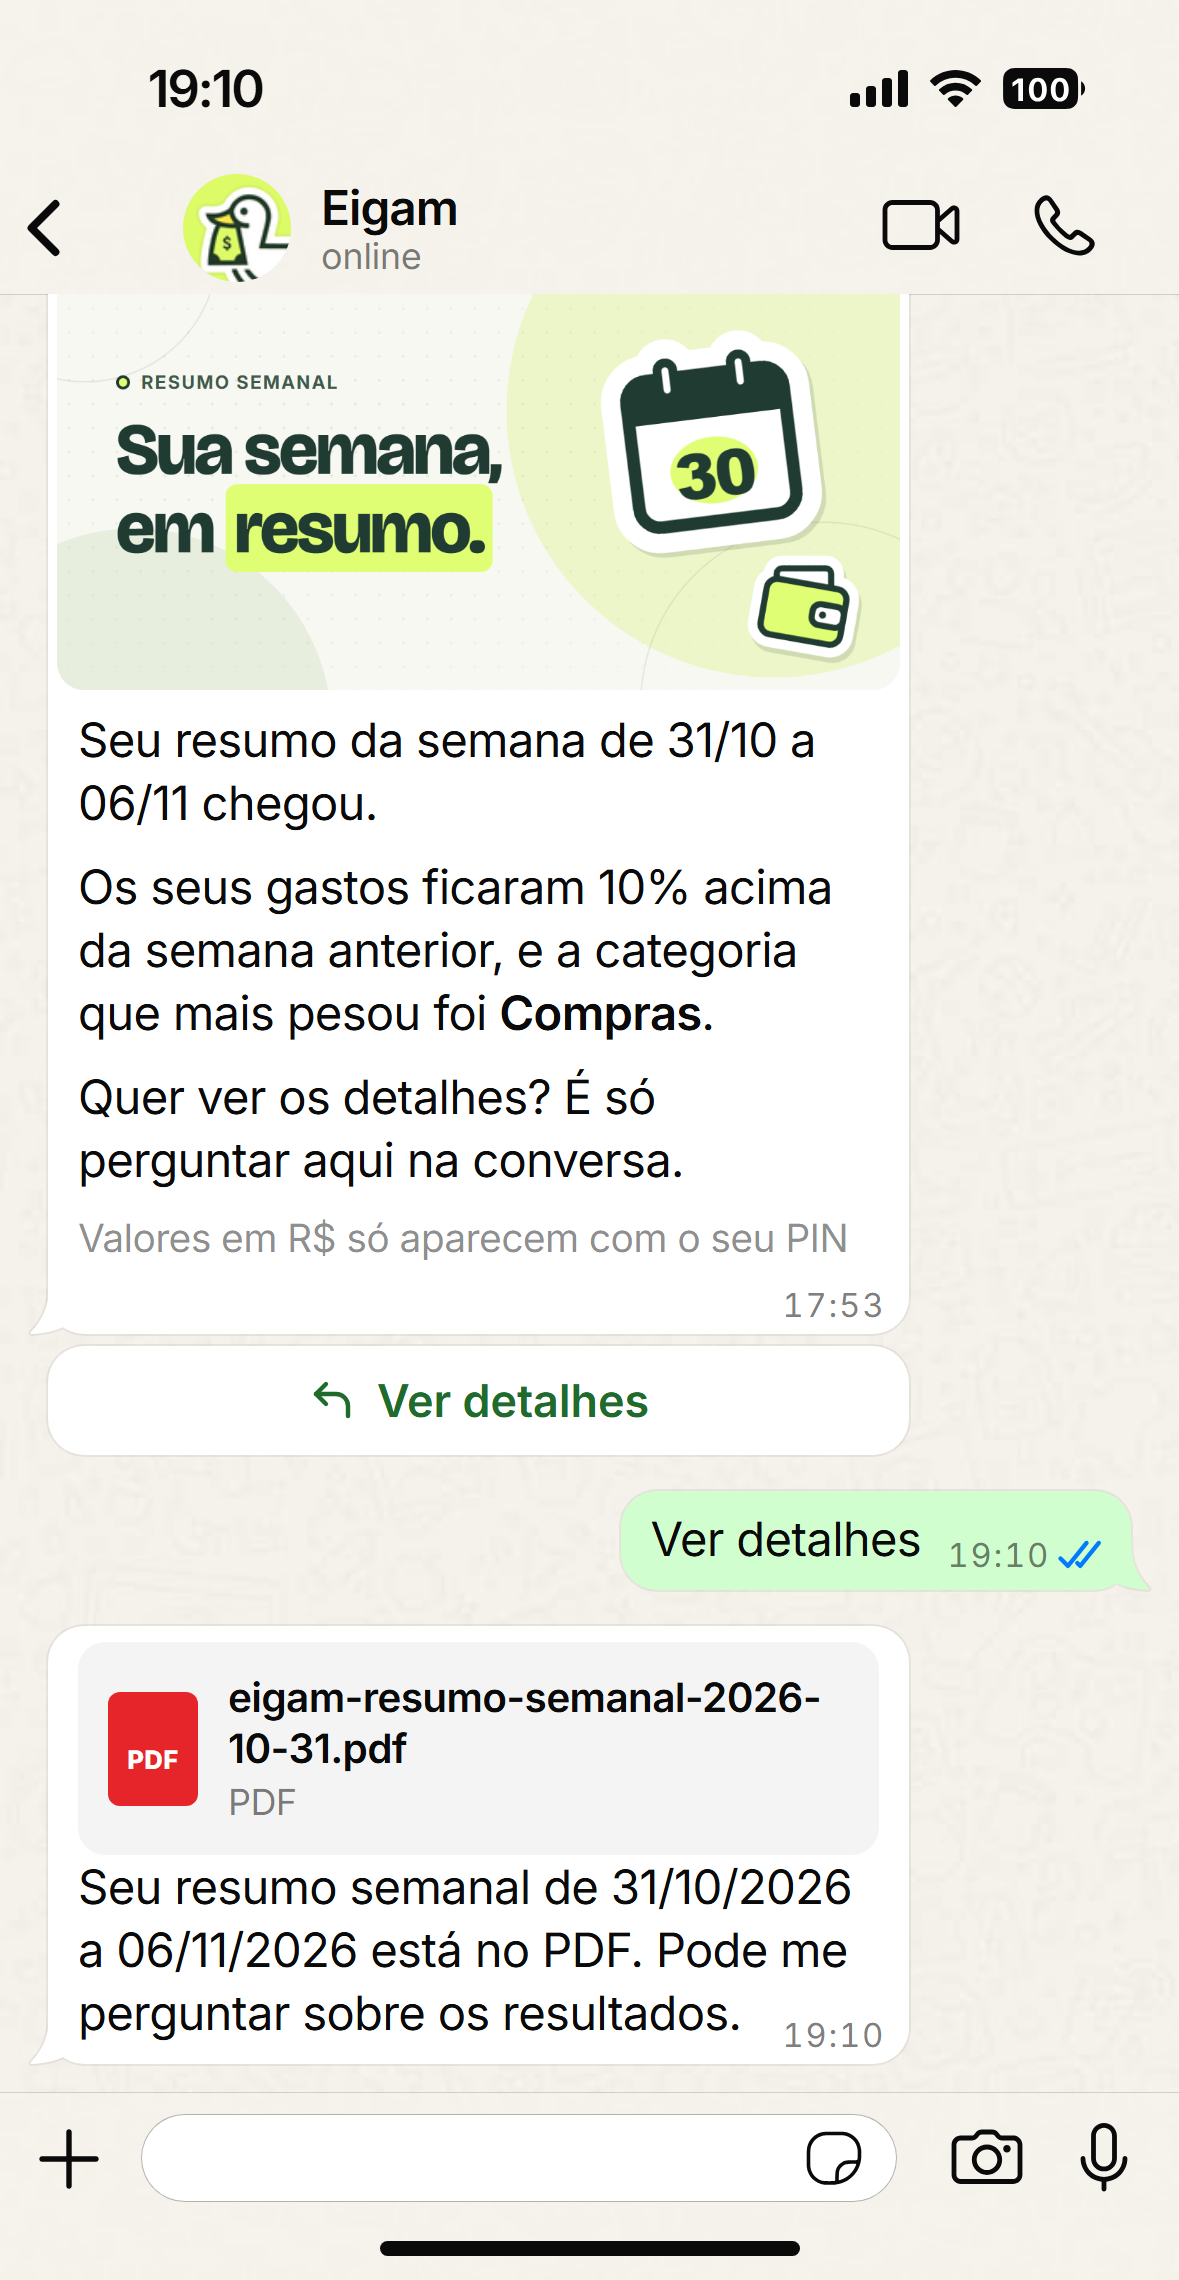
\includegraphics[width=\textwidth]{images/resultados/fluxos/fluxo_resumo_c.png}
    \end{minipage}
    \authorssource
\end{figure}

As capacidades preditivas (Figura~\ref{fig:fluxo_previsao}) apareceram na conversa com as salvaguardas descritas no Capítulo~\ref{chap:desenvolvimento}. A projeção do gasto do mês foi apresentada como faixa, com o valor já realizado, a data dos dados, as saídas deixadas de fora e a declaração de que se trata de estimativa experimental; no nono dia do mês, a largura da faixa expôs a incerteza em vez de escondê-la. Quatro minutos depois, na mesma conversa, a simulação de compra coletou valor, forma de pagamento, número de parcelas e cartão, um dado por vez, e respondeu com o efeito sobre a projeção e sobre os compromissos dos meses seguintes, sem veredito sobre comprar ou não. Quando a estimativa não está aprovada, a resposta é a abstenção: em outra conversa, a pergunta ``Quanto vai sobrar até o fim do mês?'' recebeu ``A estimativa de com quanto você fecha o mês está pausada agora''.

\begin{figure}[H]
    \centering
    \caption{Fluxo de previsões: projeção do gasto e simulação de compra}
    \label{fig:fluxo_previsao}
    \begin{minipage}[t]{0.32\textwidth}
        \centering
        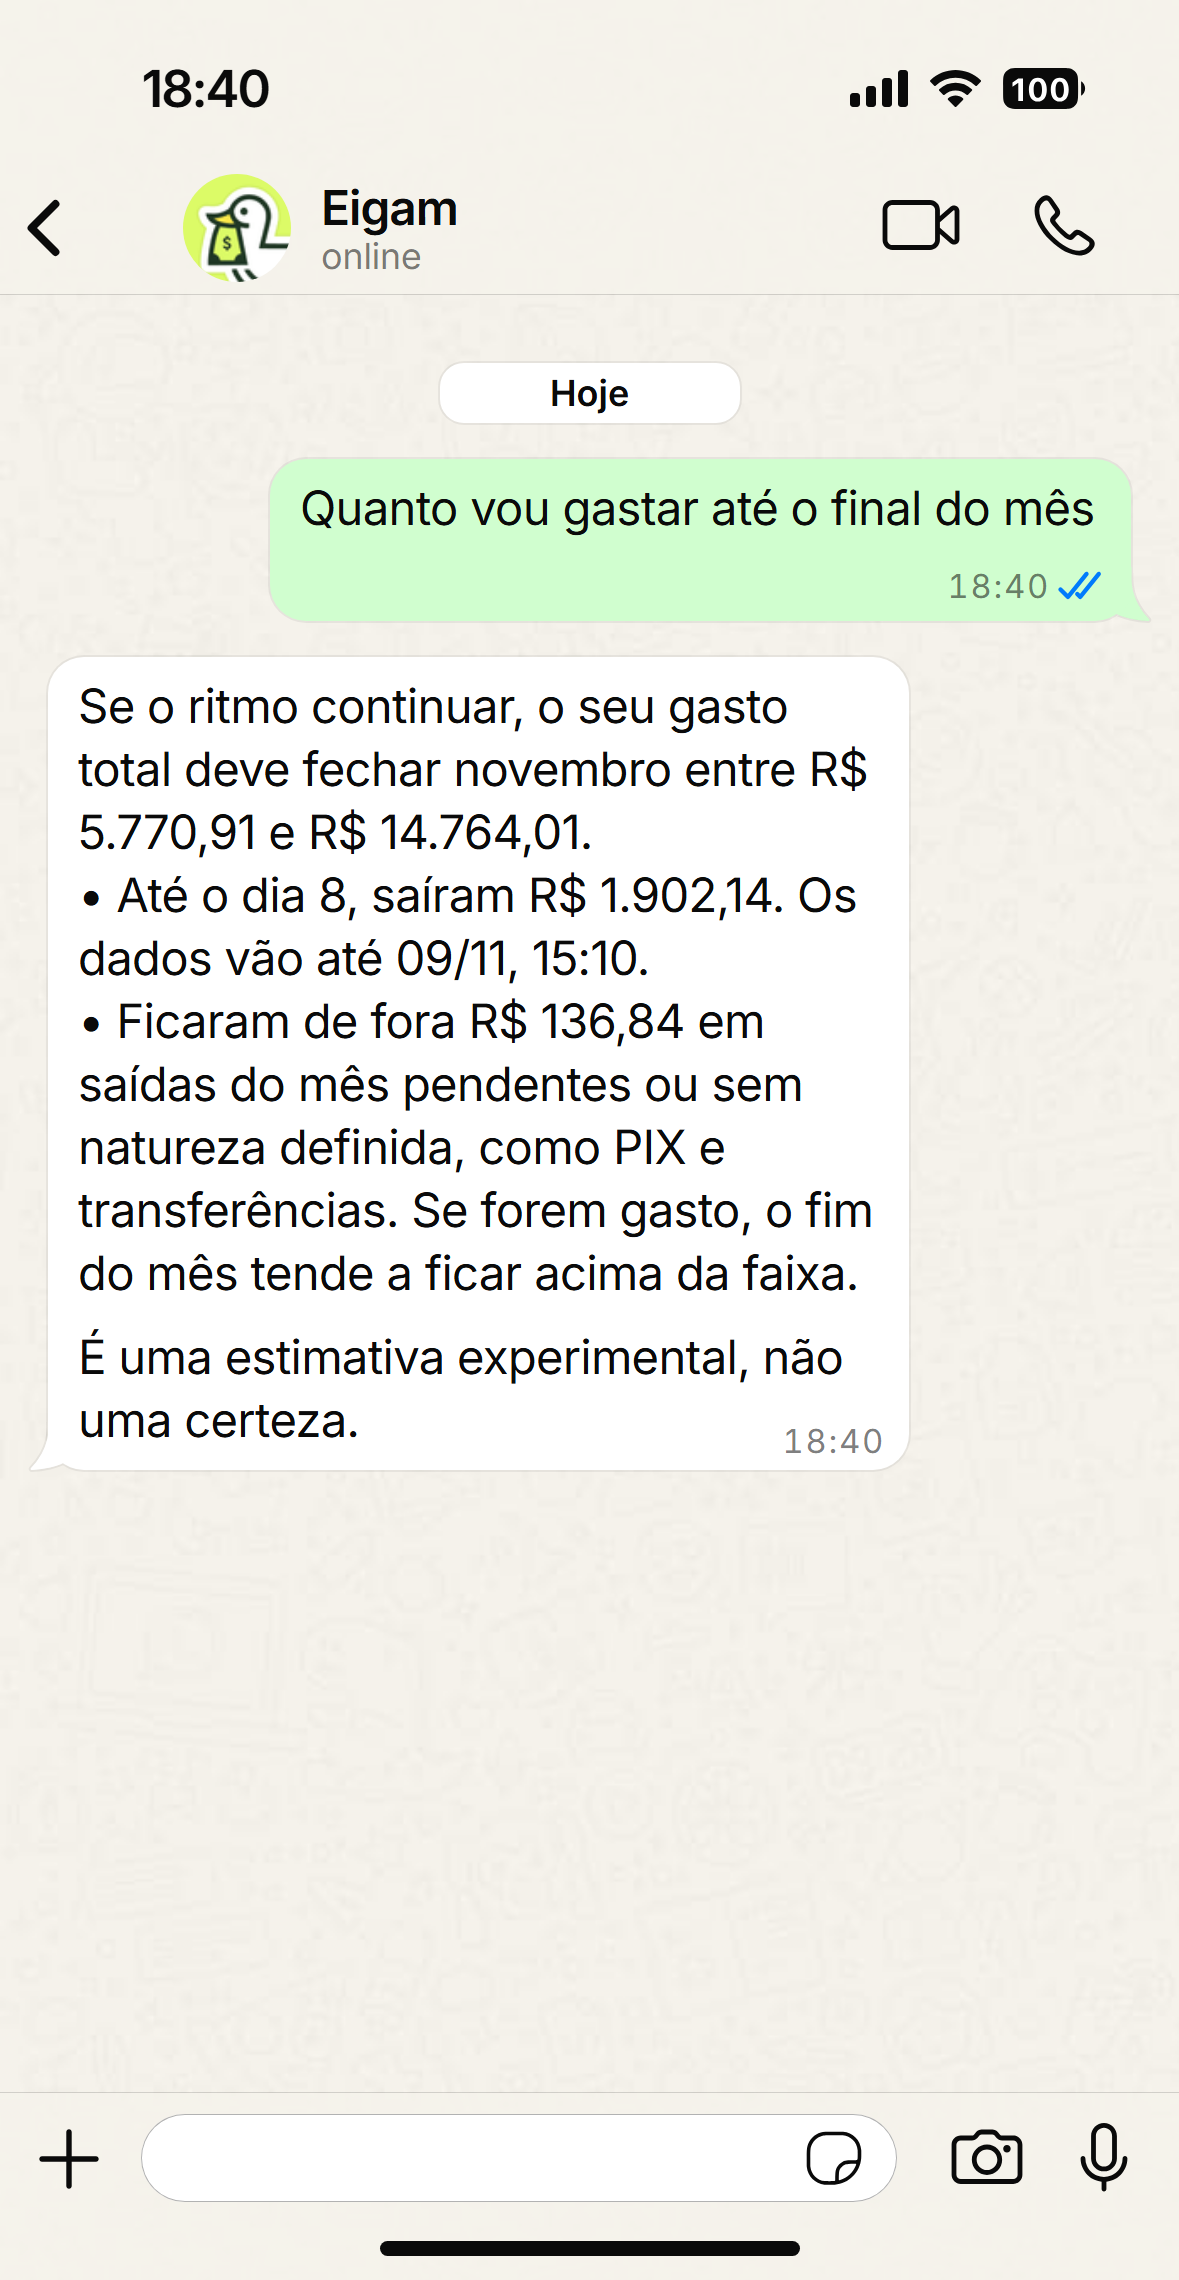
\includegraphics[width=\textwidth]{images/resultados/fluxos/fluxo_previsao_a.png}
    \end{minipage}\hfill
    \begin{minipage}[t]{0.32\textwidth}
        \centering
        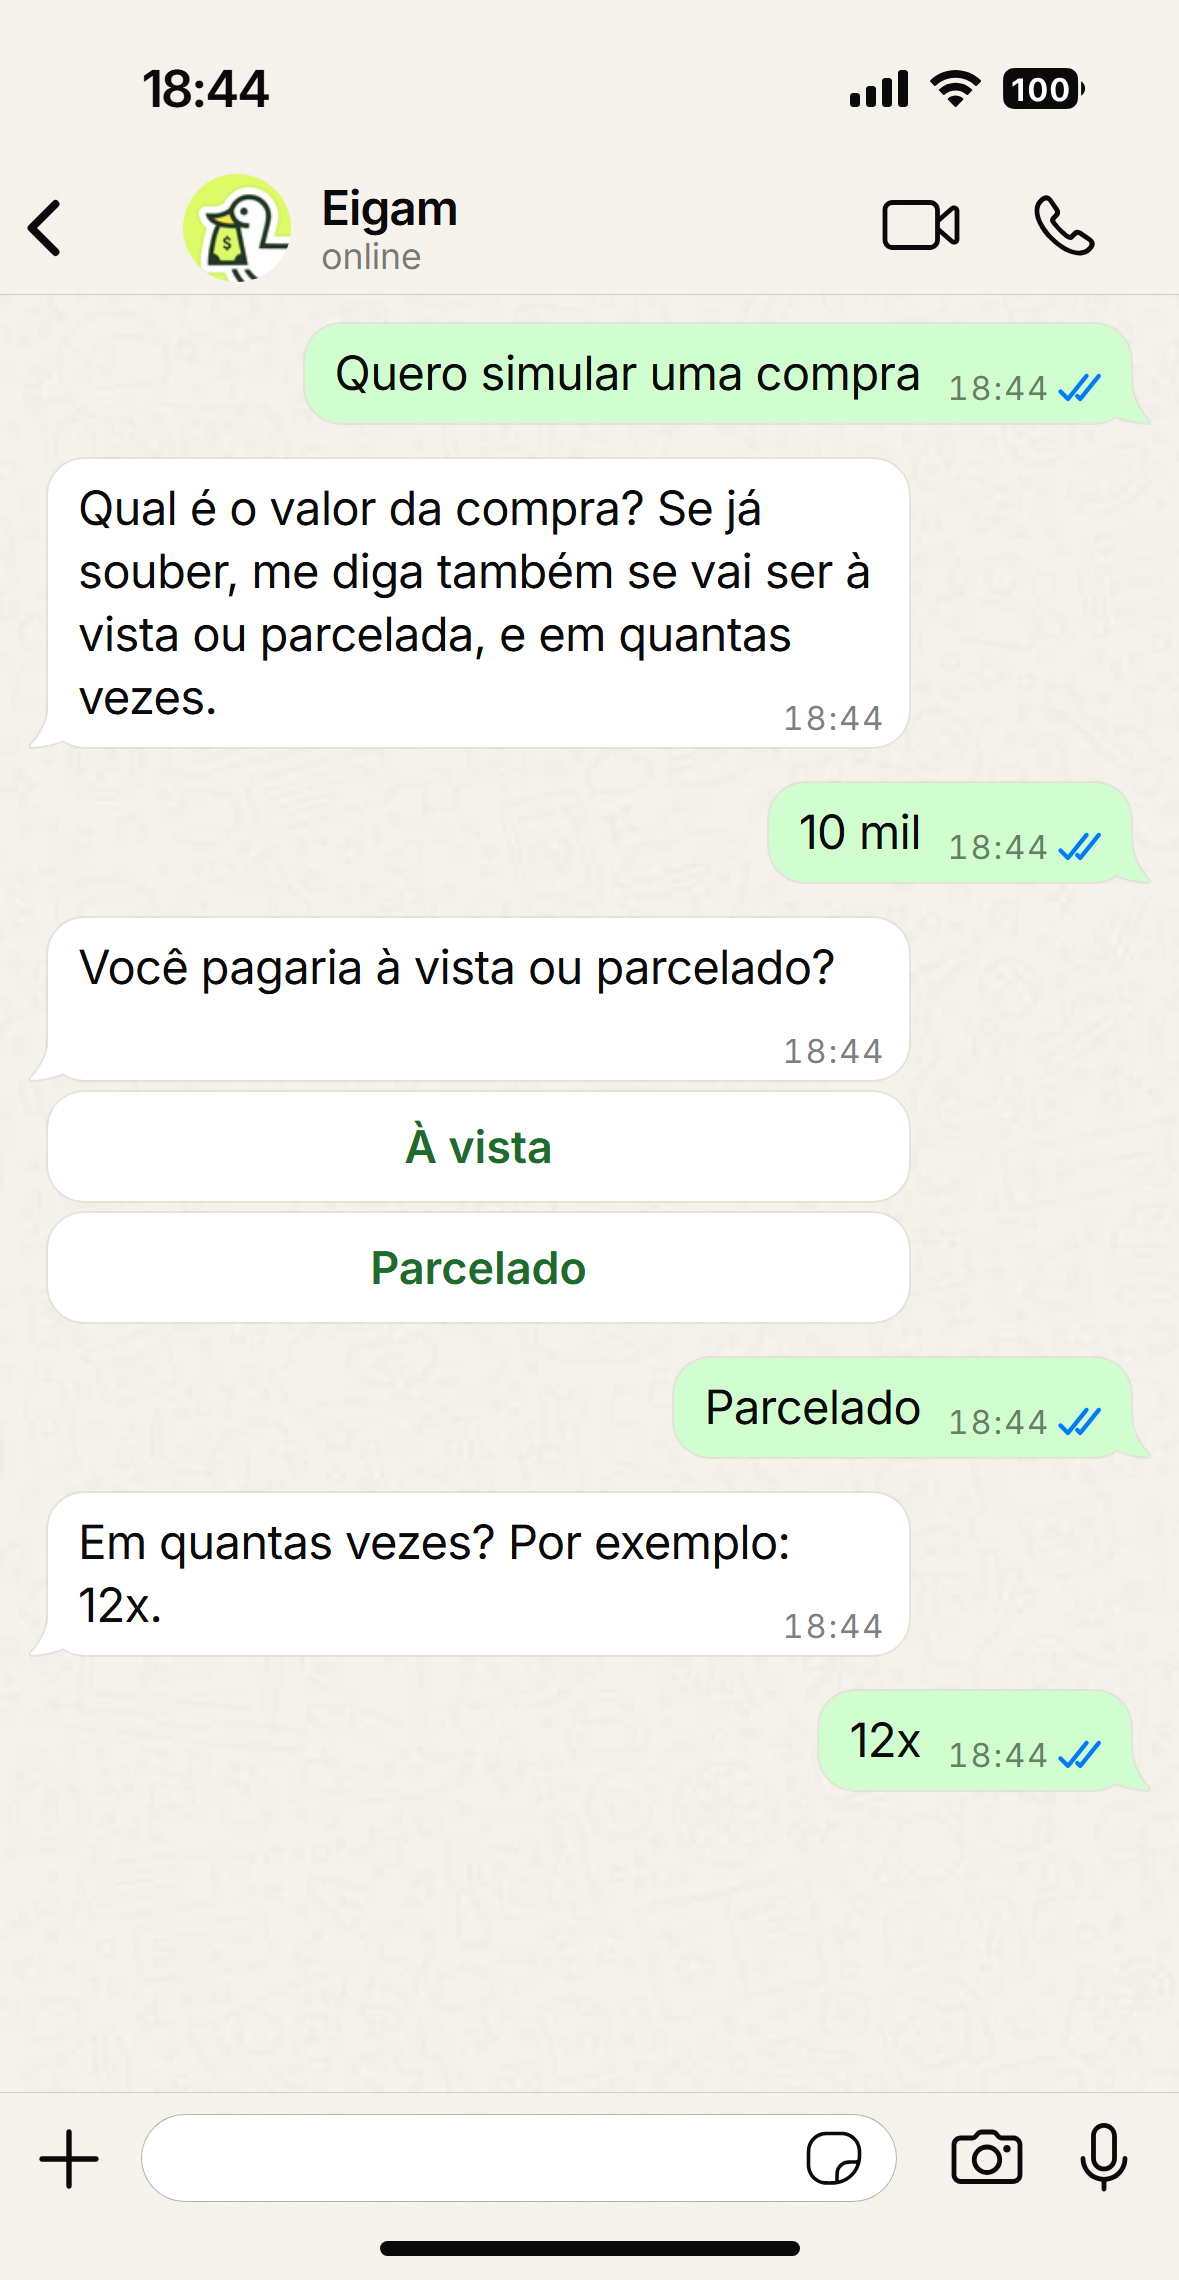
\includegraphics[width=\textwidth]{images/resultados/fluxos/fluxo_previsao_b.png}
    \end{minipage}\hfill
    \begin{minipage}[t]{0.32\textwidth}
        \centering
        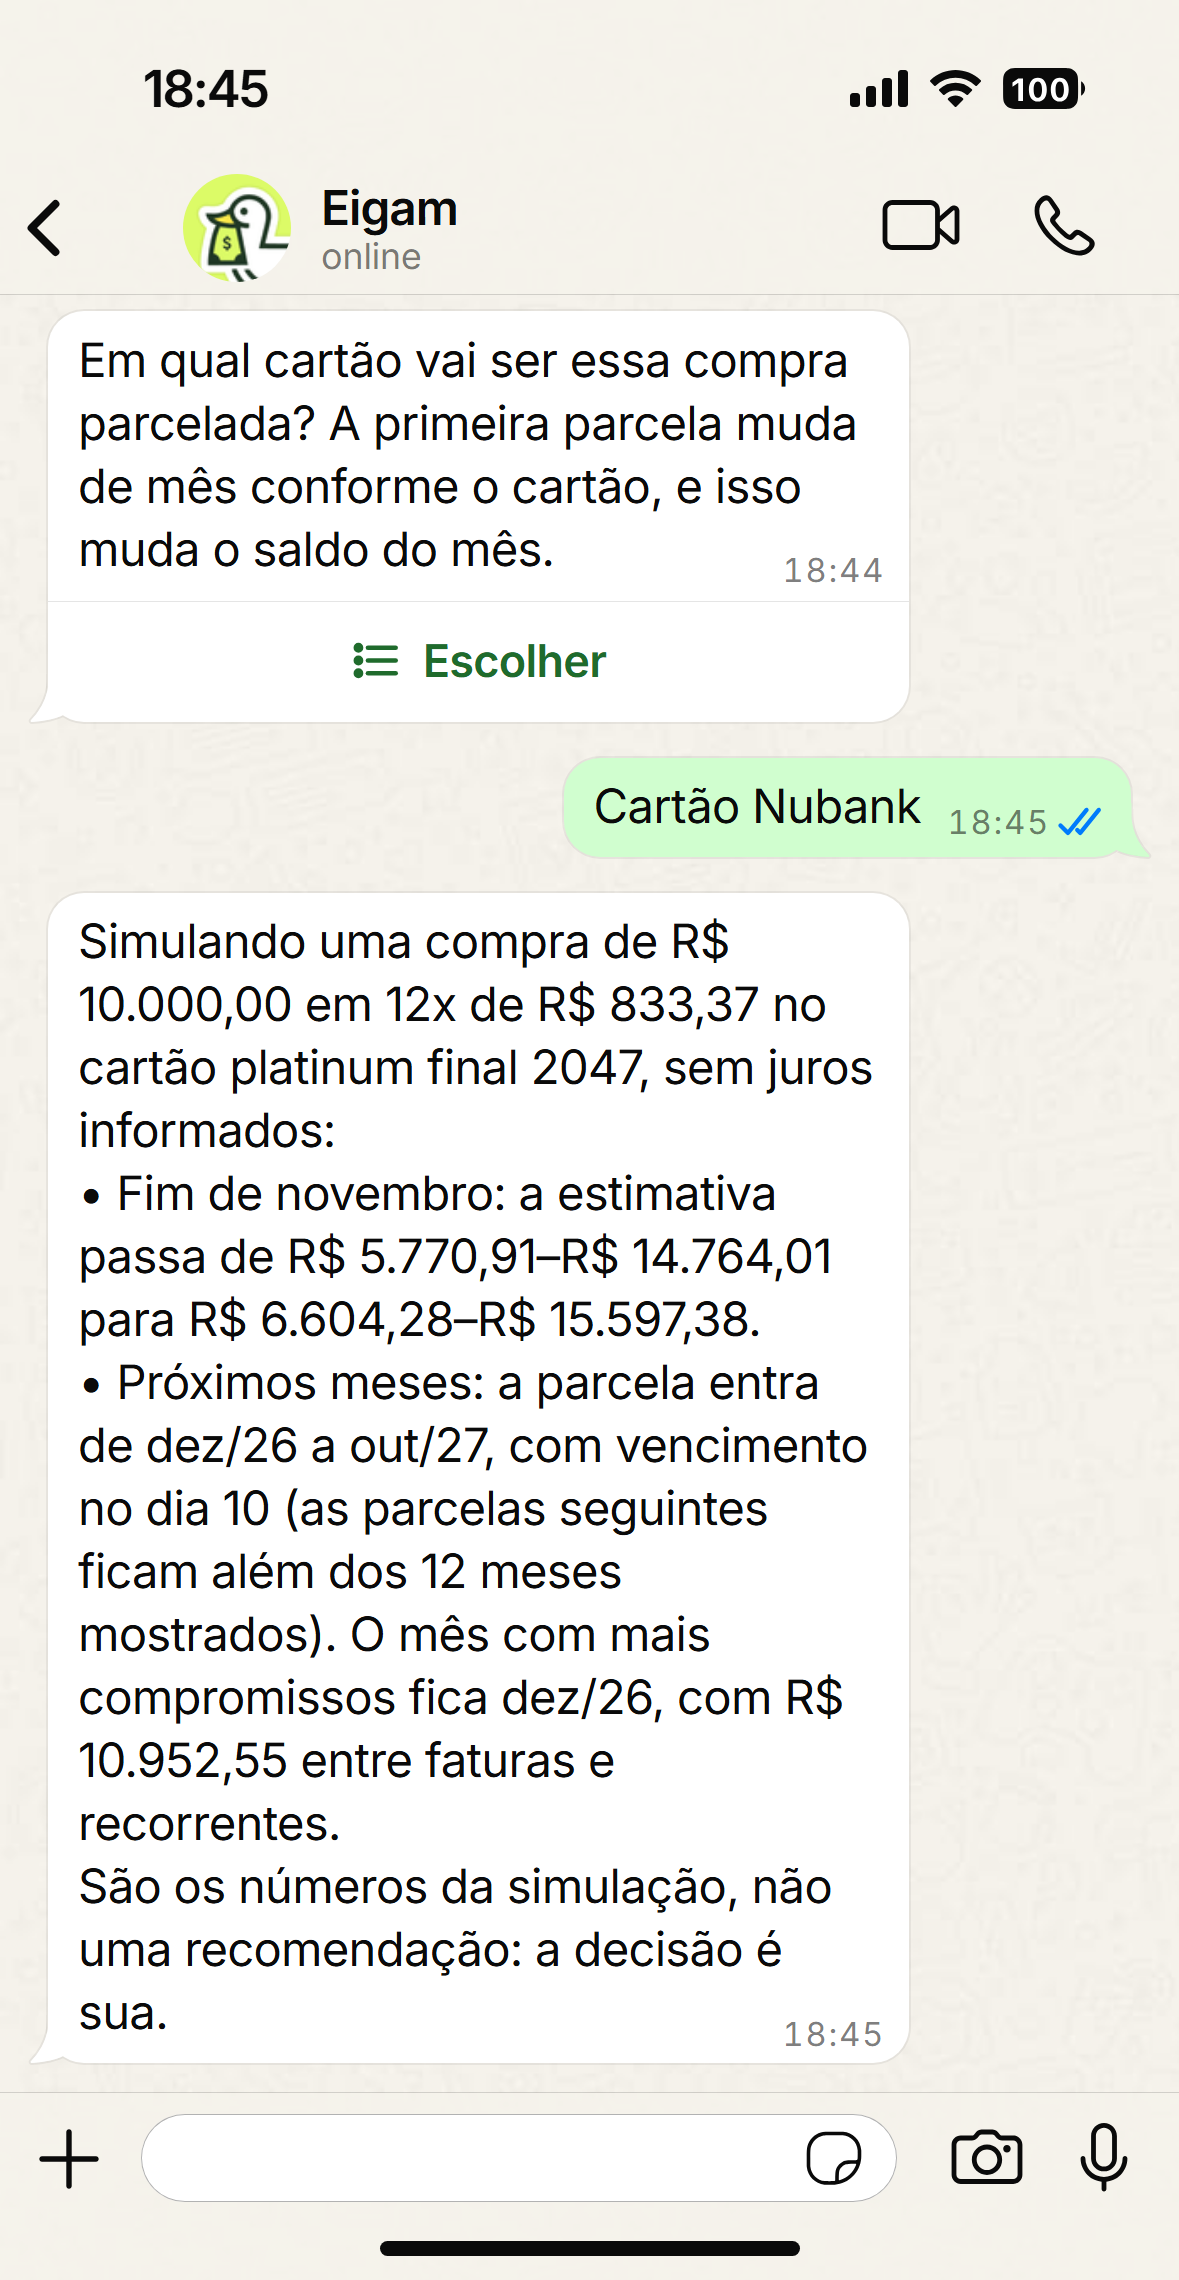
\includegraphics[width=\textwidth]{images/resultados/fluxos/fluxo_previsao_c.png}
    \end{minipage}
    \authorssource
\end{figure}

Por fim, os direitos do titular (Figura~\ref{fig:fluxo_lgpd}) foram exercidos por frases reconhecidas por regras determinísticas, com recall de 100\% medido. A pergunta ``quais dados vocês têm sobre mim?'' recebeu o inventário previsto no Art.~18, I, da LGPD: o que é guardado e como é protegido, a base legal, a finalidade, os prazos, quem trata os dados junto com a solução e a situação atual da conta. Em seguida, o pedido de exportação foi registrado e o arquivo em JSON chegou no próprio canal, sem links externos. A exclusão segue o mesmo caminho, com confirmação explícita, e revoga as conexões bancárias, anonimiza as transações e apaga os dados derivados.

\begin{figure}[H]
    \centering
    \caption{Fluxo dos direitos do titular pela conversa}
    \label{fig:fluxo_lgpd}
    \begin{minipage}[t]{0.32\textwidth}
        \centering
        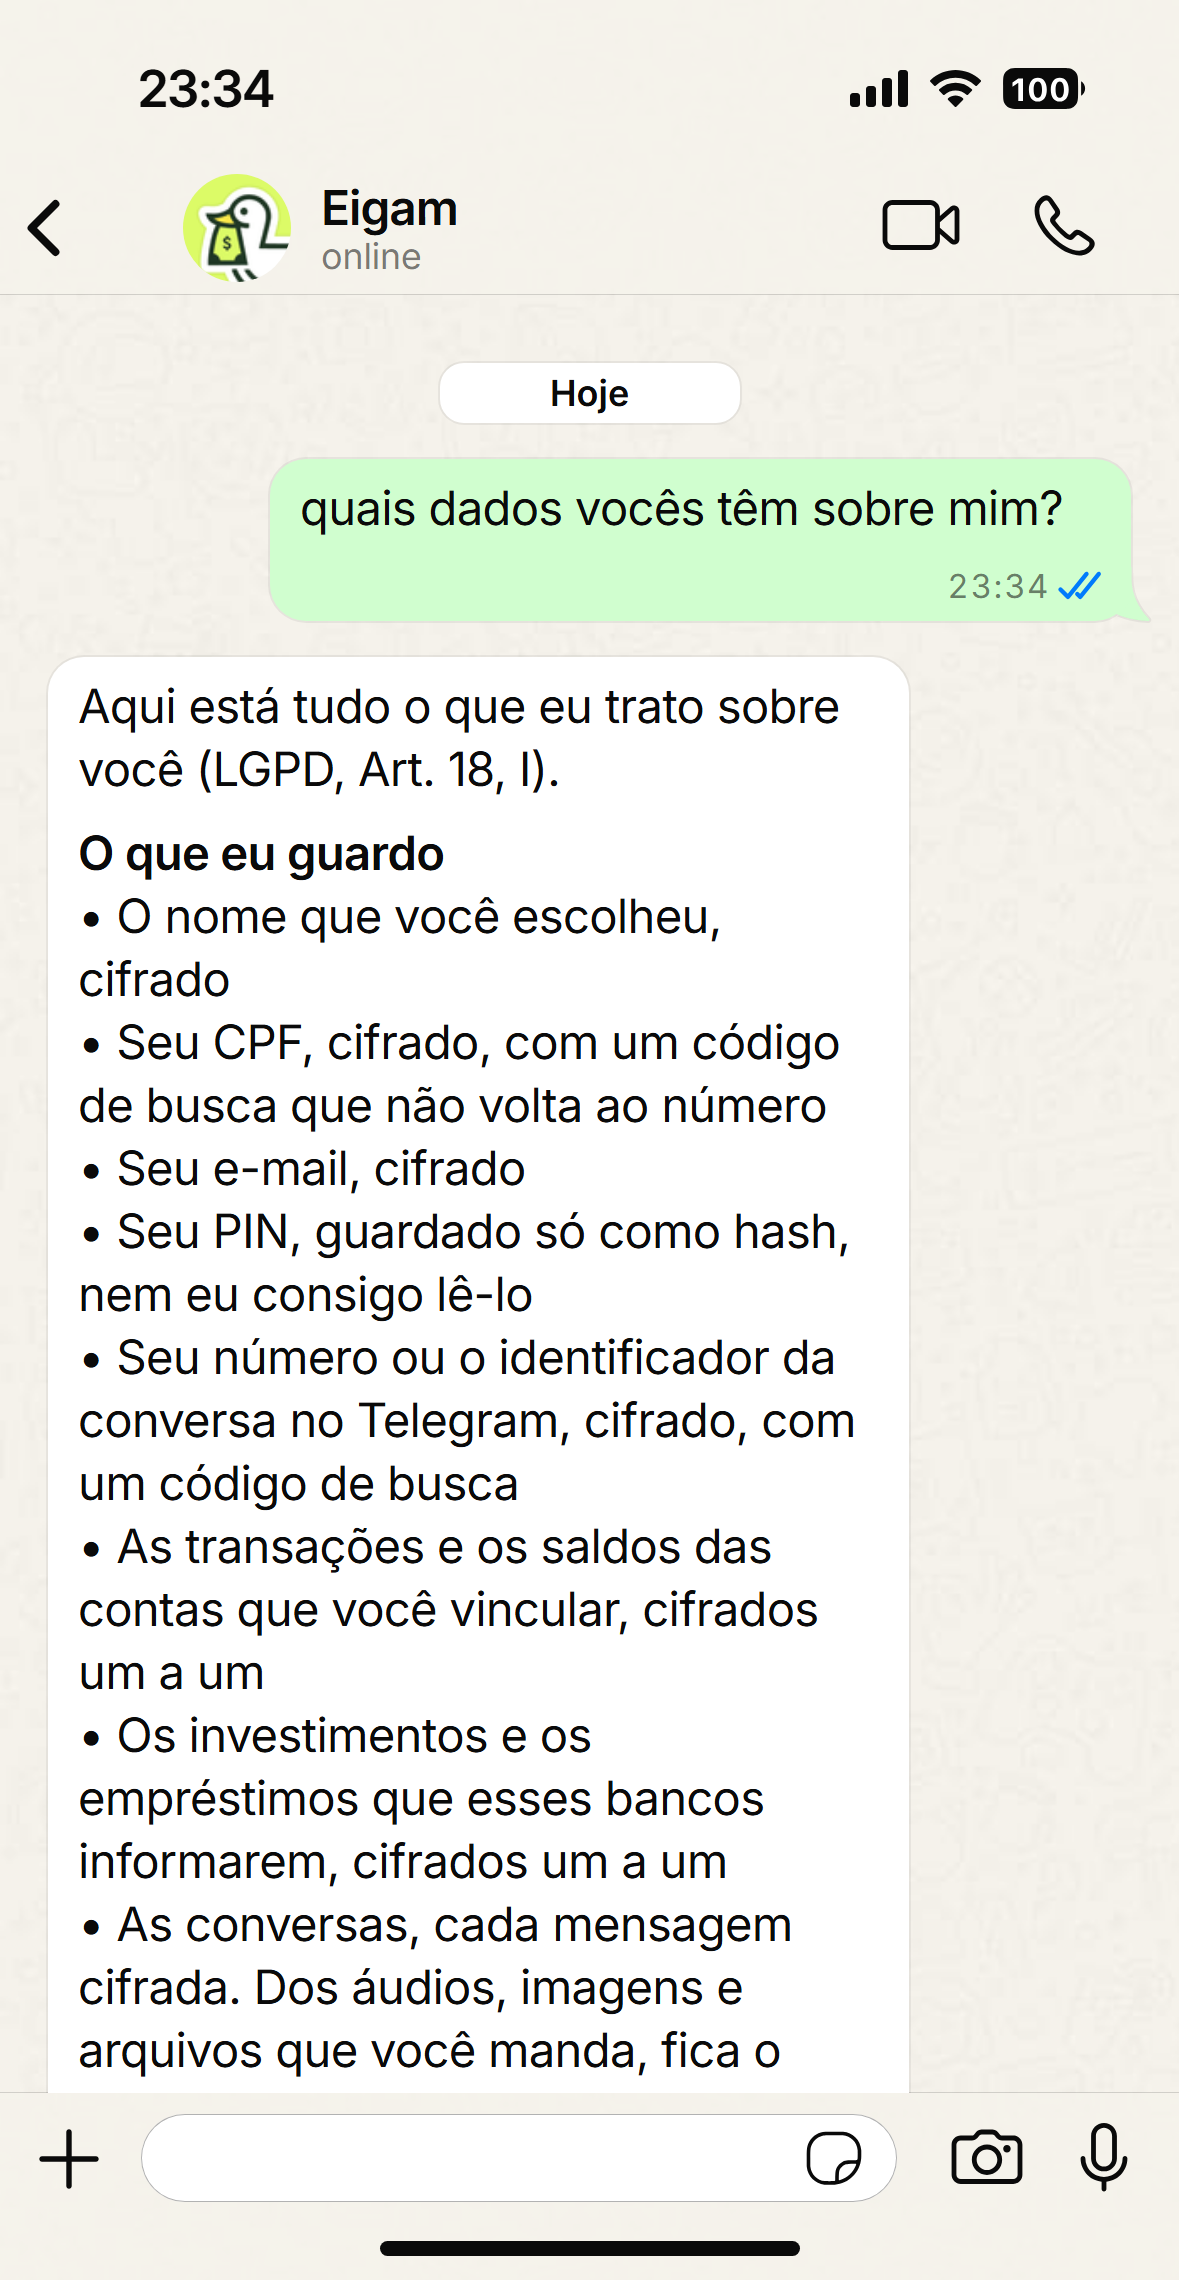
\includegraphics[width=\textwidth]{images/resultados/fluxos/fluxo_lgpd_a.png}
    \end{minipage}\hfill
    \begin{minipage}[t]{0.32\textwidth}
        \centering
        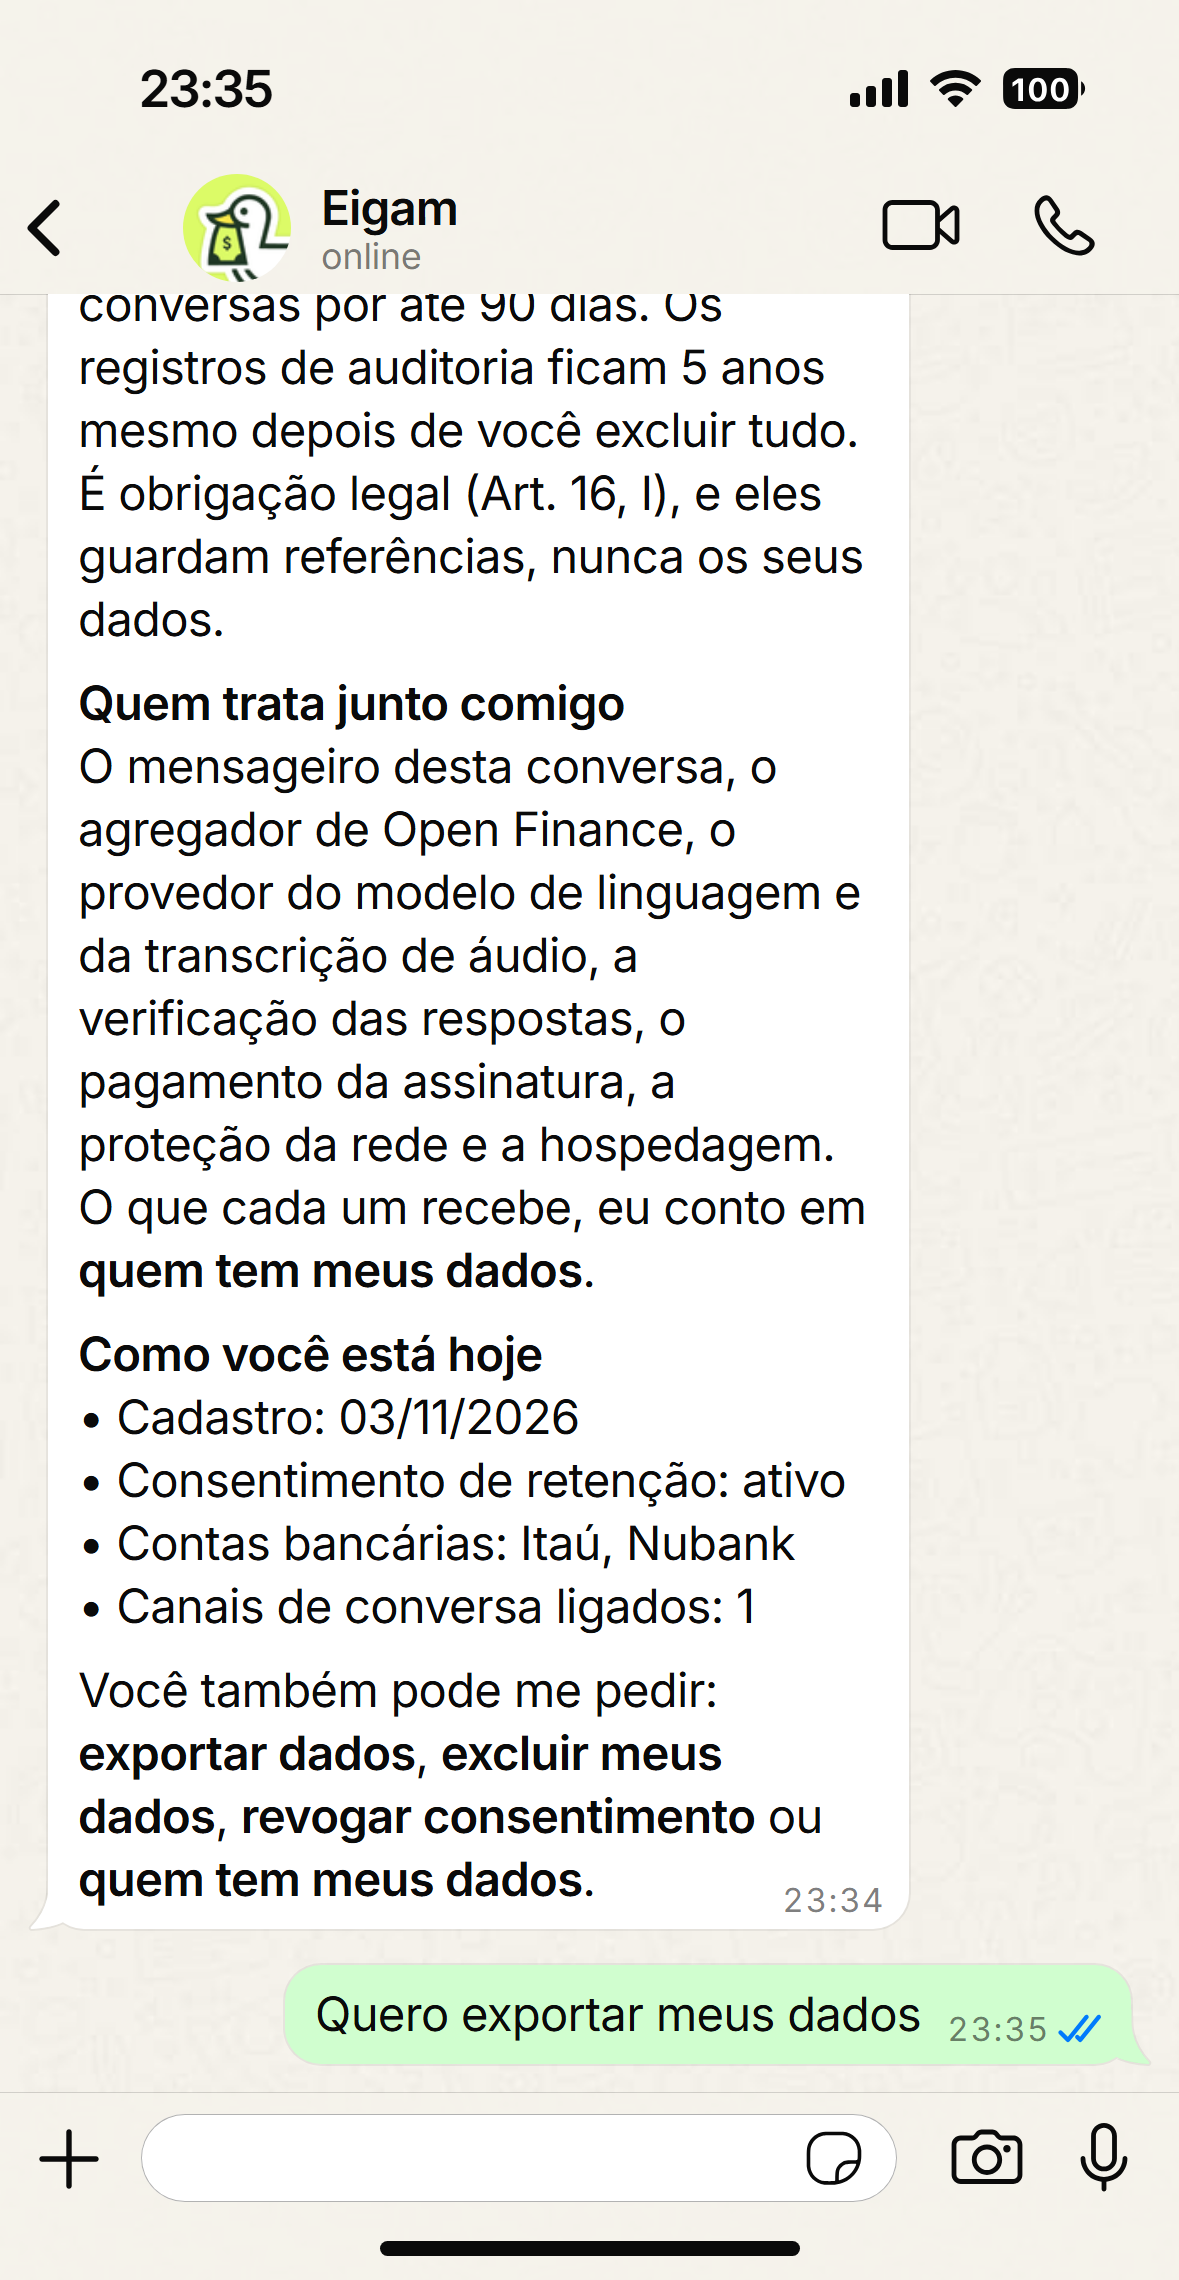
\includegraphics[width=\textwidth]{images/resultados/fluxos/fluxo_lgpd_b.png}
    \end{minipage}\hfill
    \begin{minipage}[t]{0.32\textwidth}
        \centering
        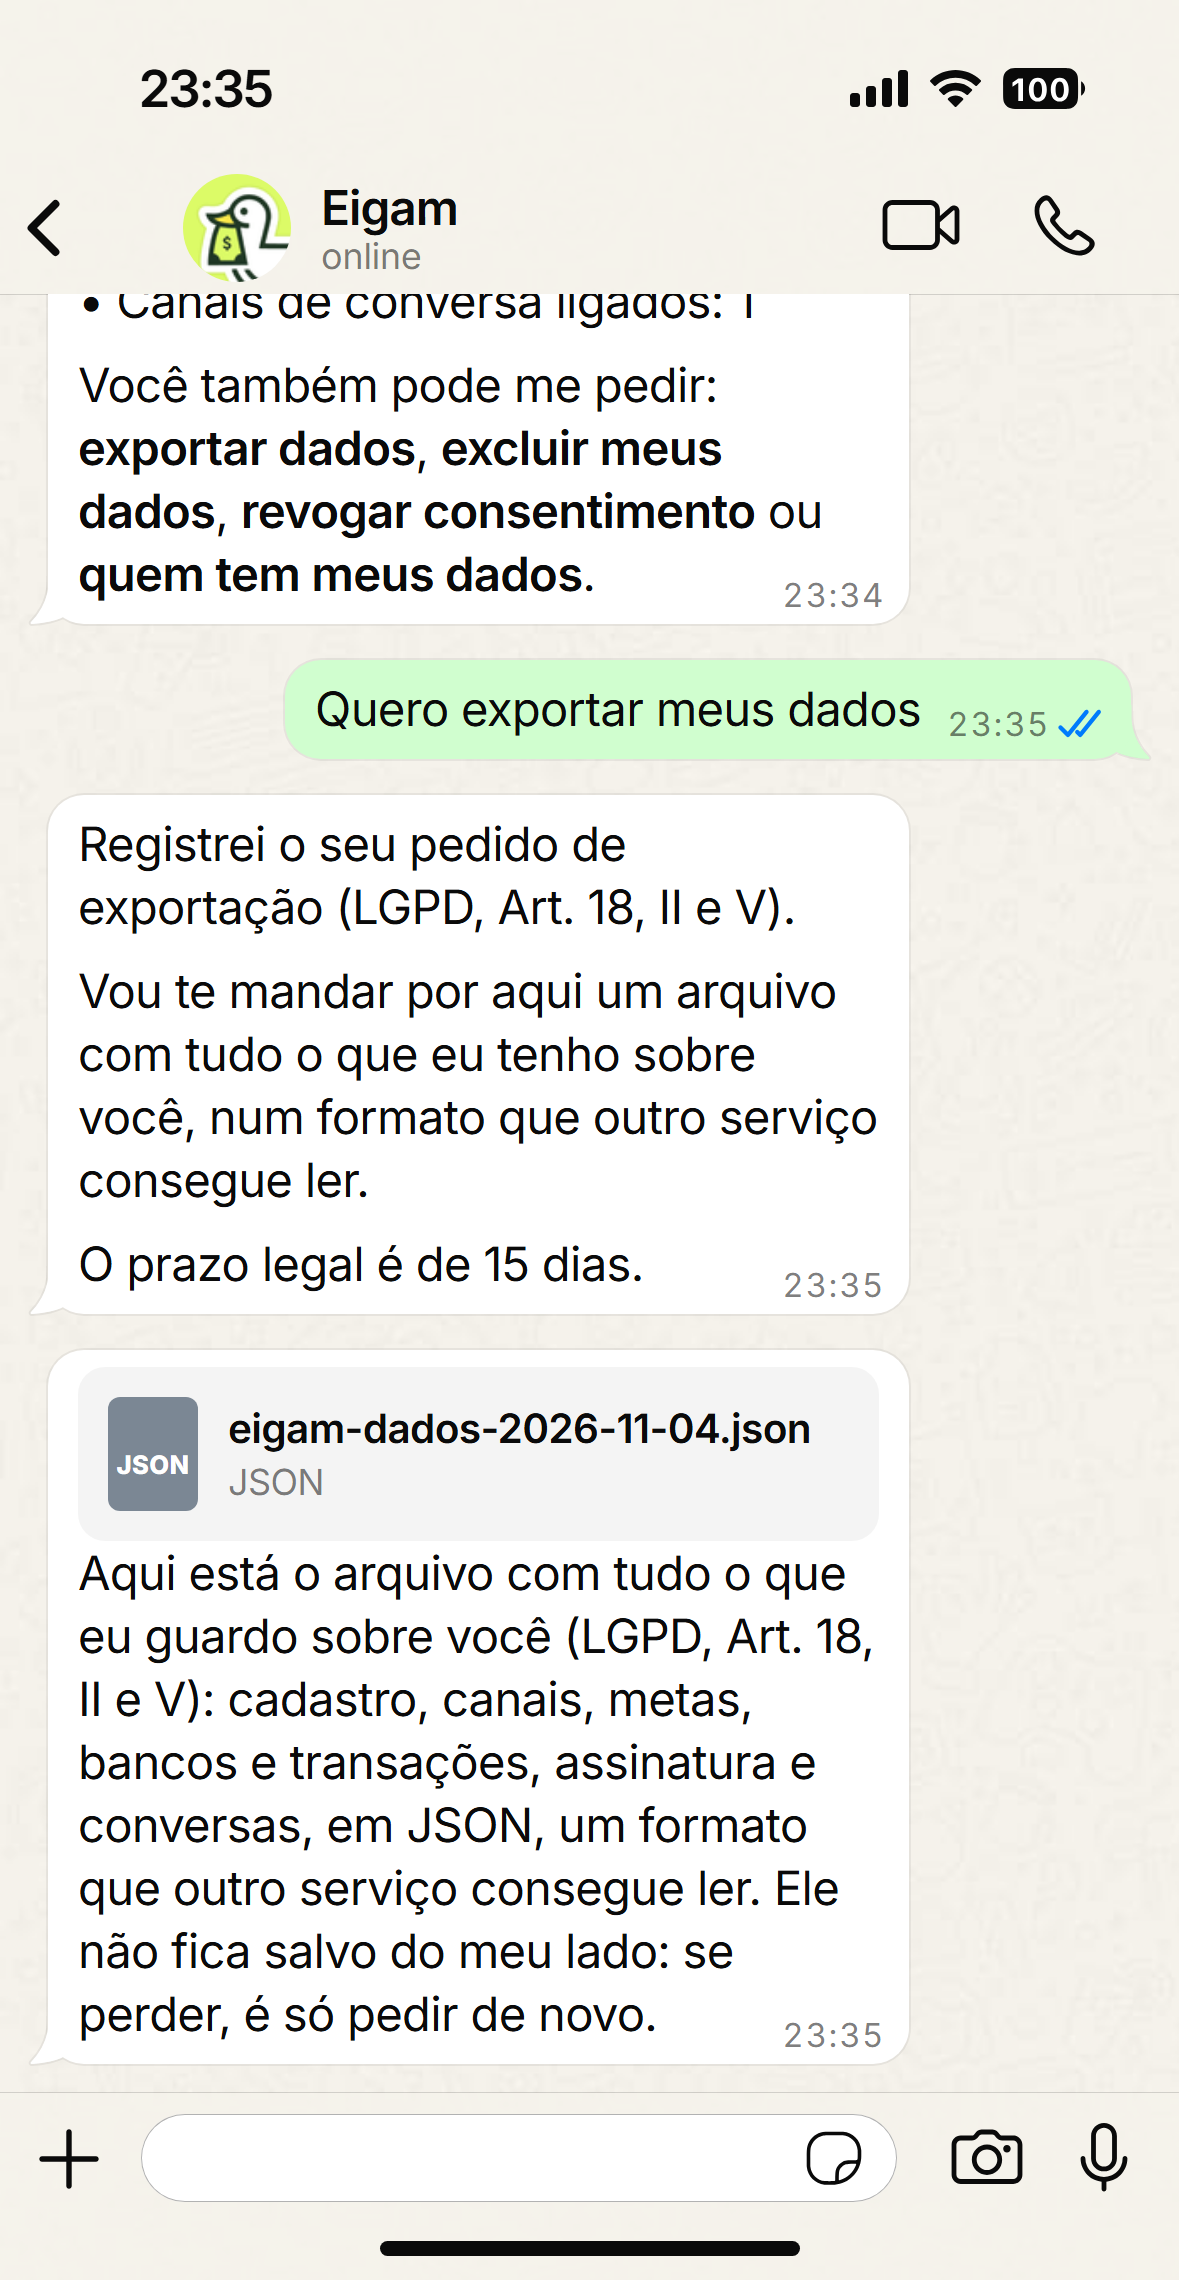
\includegraphics[width=\textwidth]{images/resultados/fluxos/fluxo_lgpd_c.png}
    \end{minipage}
    \authorssource
\end{figure}

\subsection{Formulários nos Canais}

Onze formulários cobrem as tarefas que pedem dados estruturados: cadastro, entrada por outro aplicativo, conexão de banco, meta, orçamento, preferências de aviso, direitos do titular, liberação de valores, troca de PIN, plano Pro e avaliação. Cada formulário é definido uma única vez e traduzido pelo adaptador de cada canal: no \textit{WhatsApp}, vira um \textit{WhatsApp Flow}, uma folha nativa aberta sobre a conversa e trocada com o \textit{gateway} por um \textit{endpoint} cifrado; no \textit{Telegram}, vira um Mini App, que adota as cores do tema do próprio usuário. As Figuras~\ref{fig:form_cadastro} a~\ref{fig:form_preferencias} mostram quatro desses formulários no \textit{WhatsApp}: a mensagem que oferece o formulário, a folha aberta sobre a conversa e, quando cabe, a confirmação que volta para ela.

\begin{figure}[H]
    \centering
    \caption{Cadastro pelo formulário do \textit{WhatsApp Flows}}
    \label{fig:form_cadastro}
    \begin{minipage}[t]{0.32\textwidth}
        \centering
        
\includegraphics[width=\textwidth]{images/resultados/fluxos/form_cadastro_a.png}
    \end{minipage}\hfill
    \begin{minipage}[t]{0.32\textwidth}
        \centering
        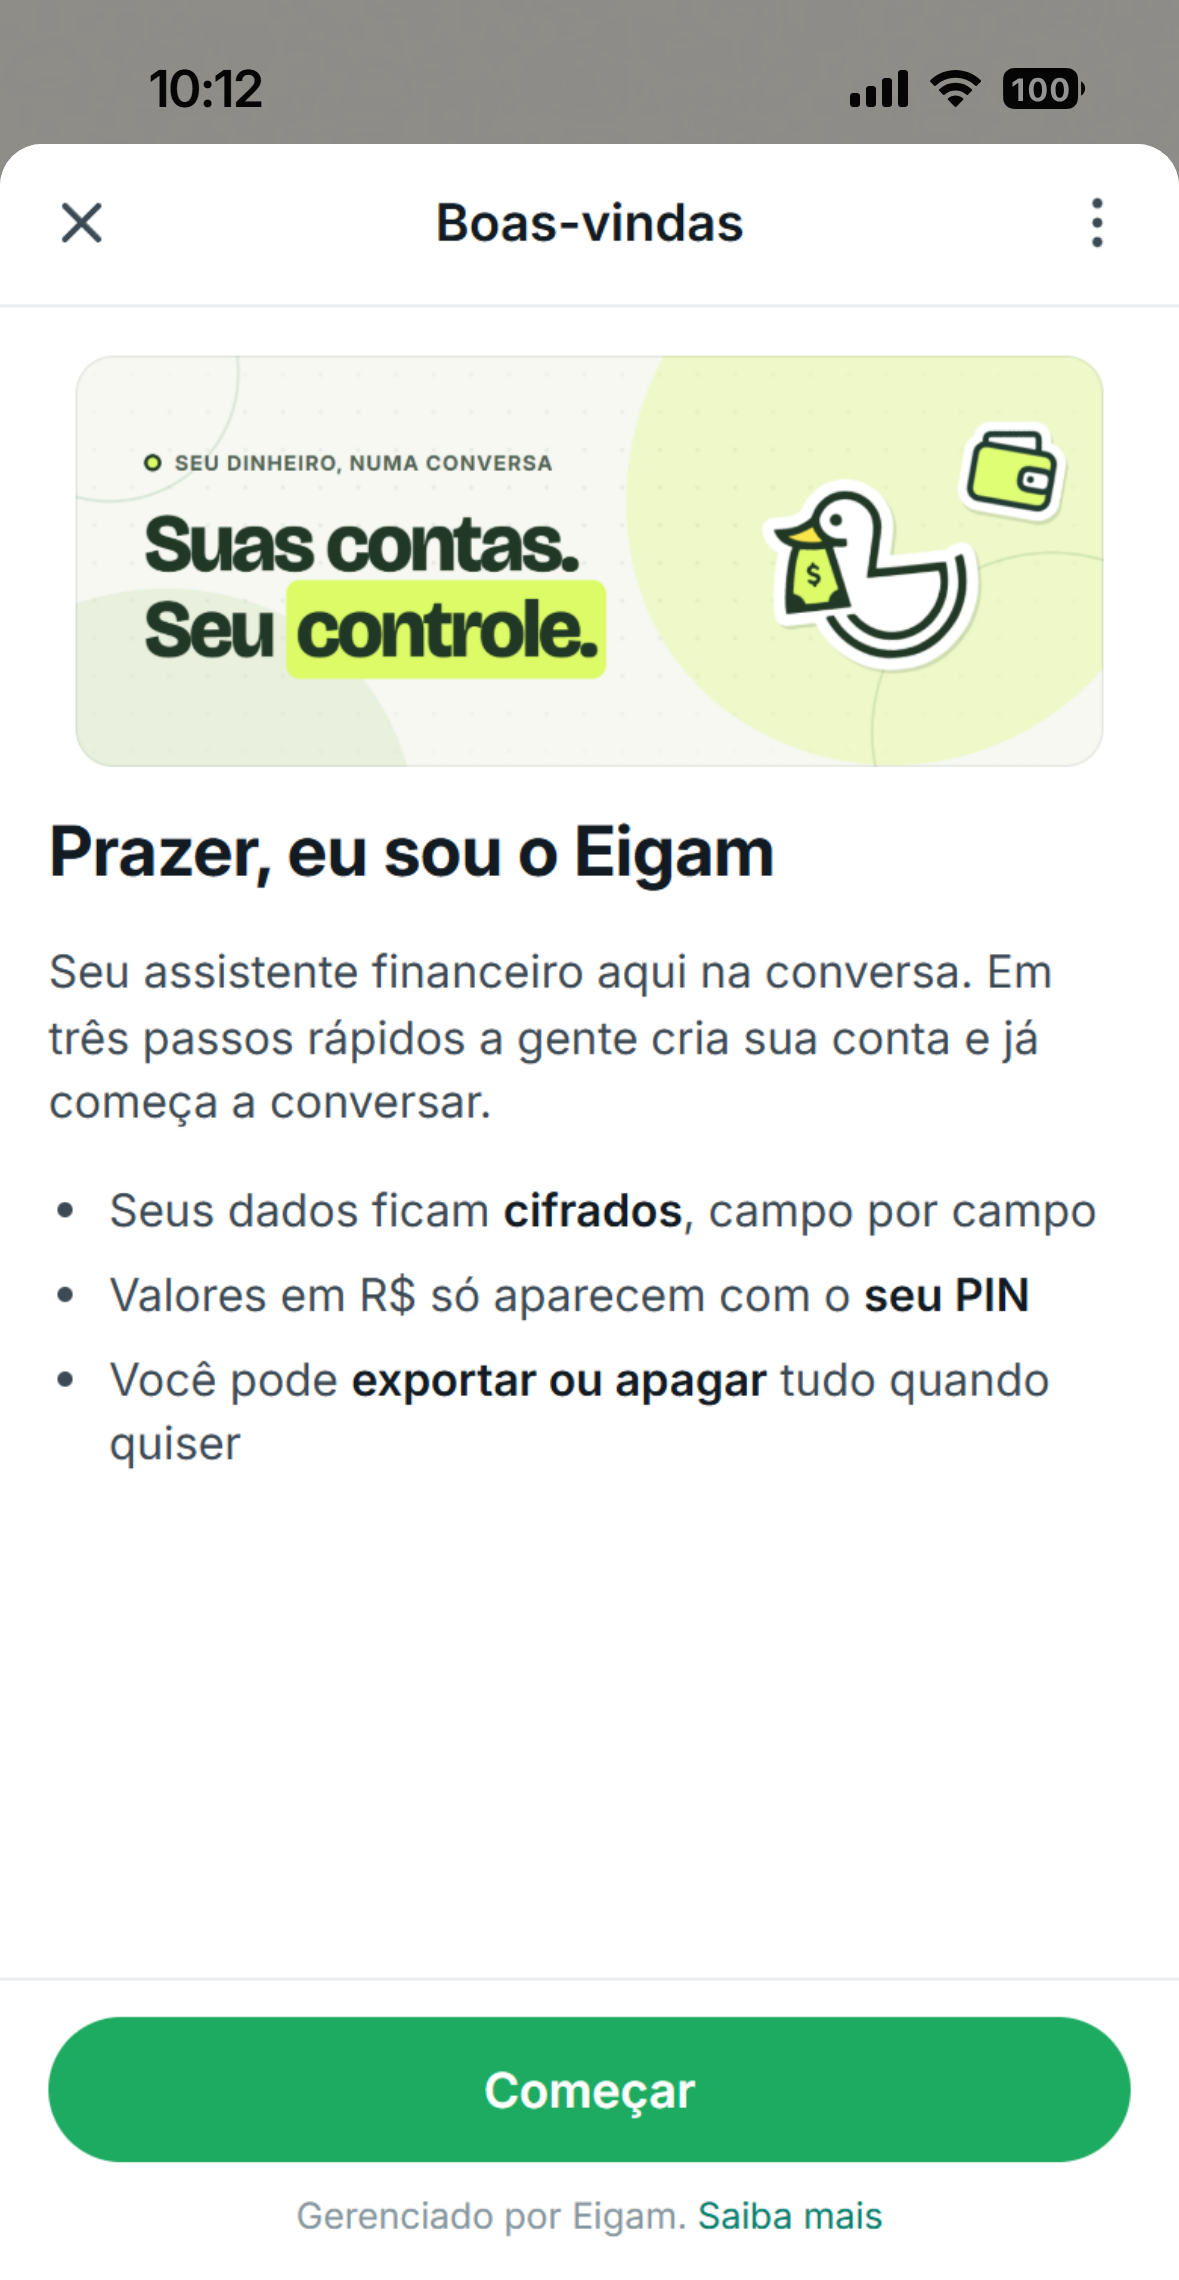
\includegraphics[width=\textwidth]{images/resultados/fluxos/form_cadastro_b.png}
    \end{minipage}\hfill
    \begin{minipage}[t]{0.32\textwidth}
        \centering
        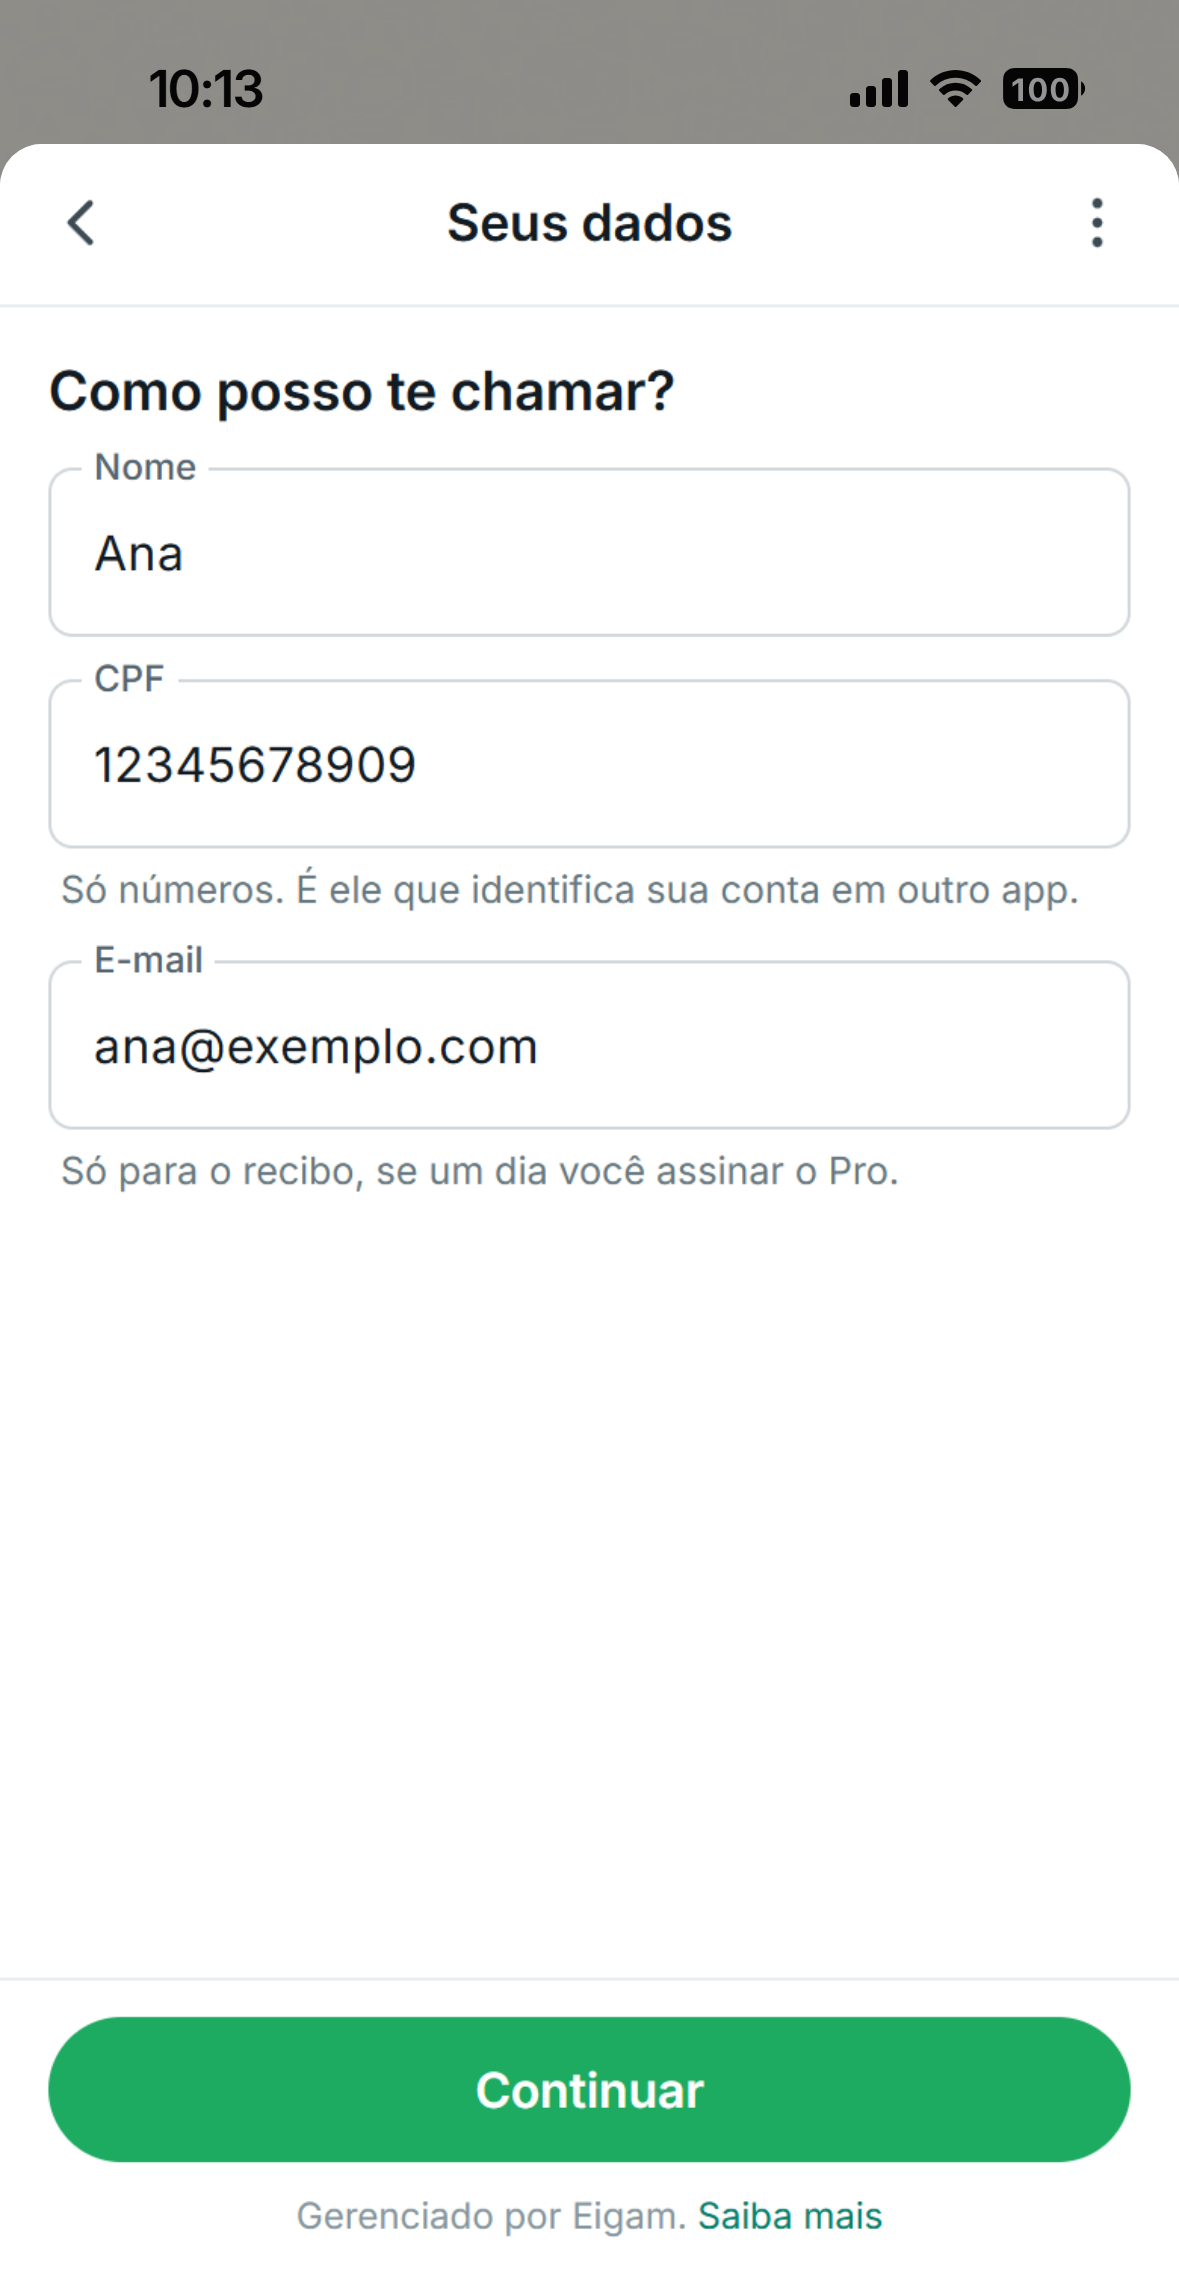
\includegraphics[width=\textwidth]{images/resultados/fluxos/form_cadastro_c.png}
    \end{minipage}
    \par\medskip
    \begin{minipage}[t]{0.32\textwidth}
        \centering
        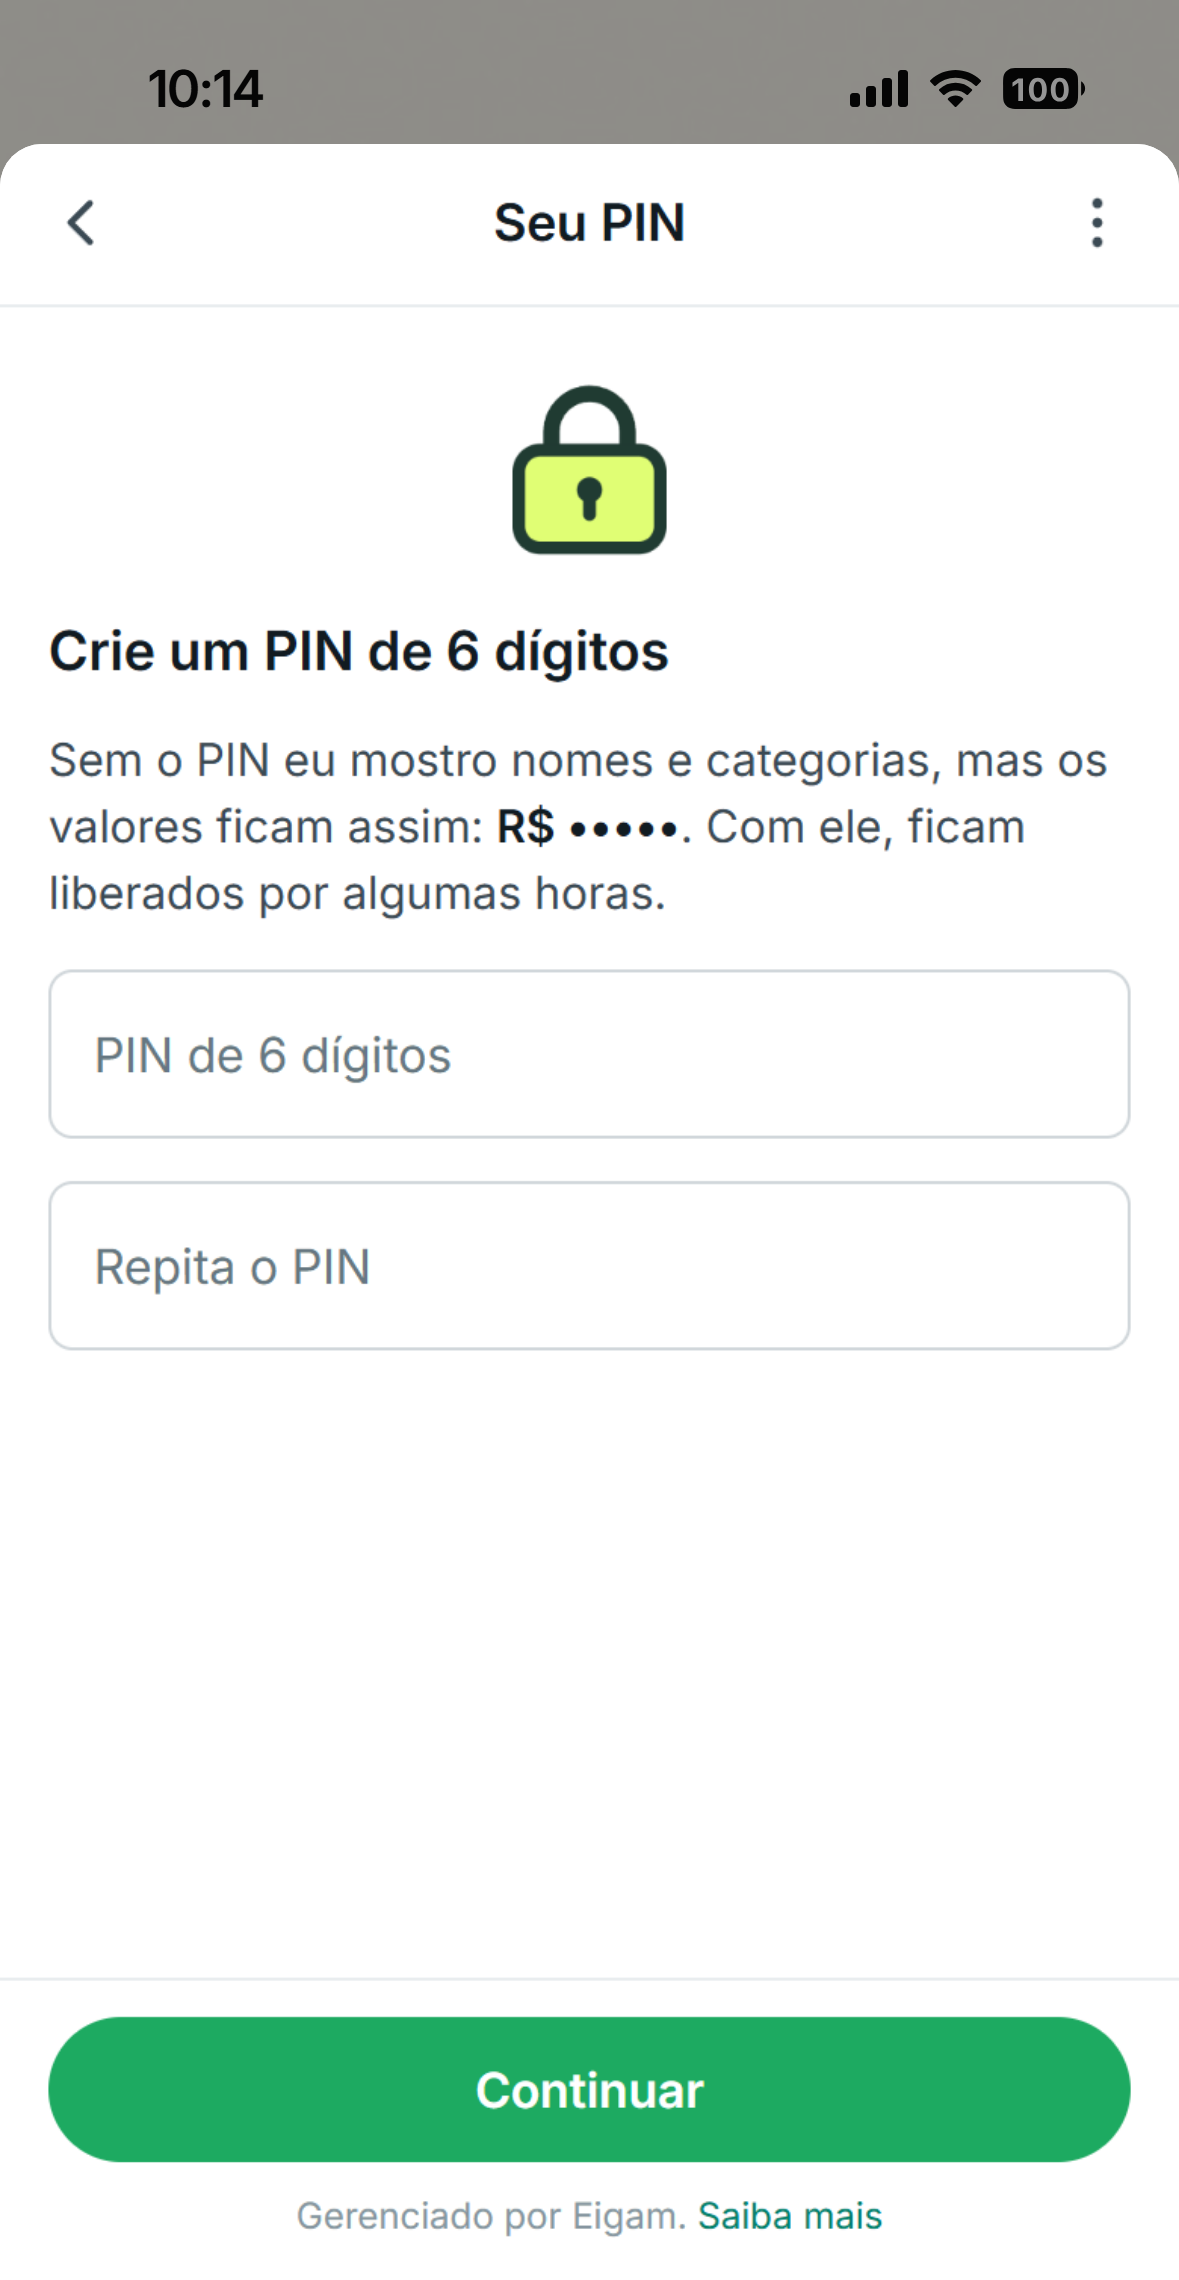
\includegraphics[width=\textwidth]{images/resultados/fluxos/form_cadastro_d.png}
    \end{minipage}\hfill
    \begin{minipage}[t]{0.32\textwidth}
        \centering
        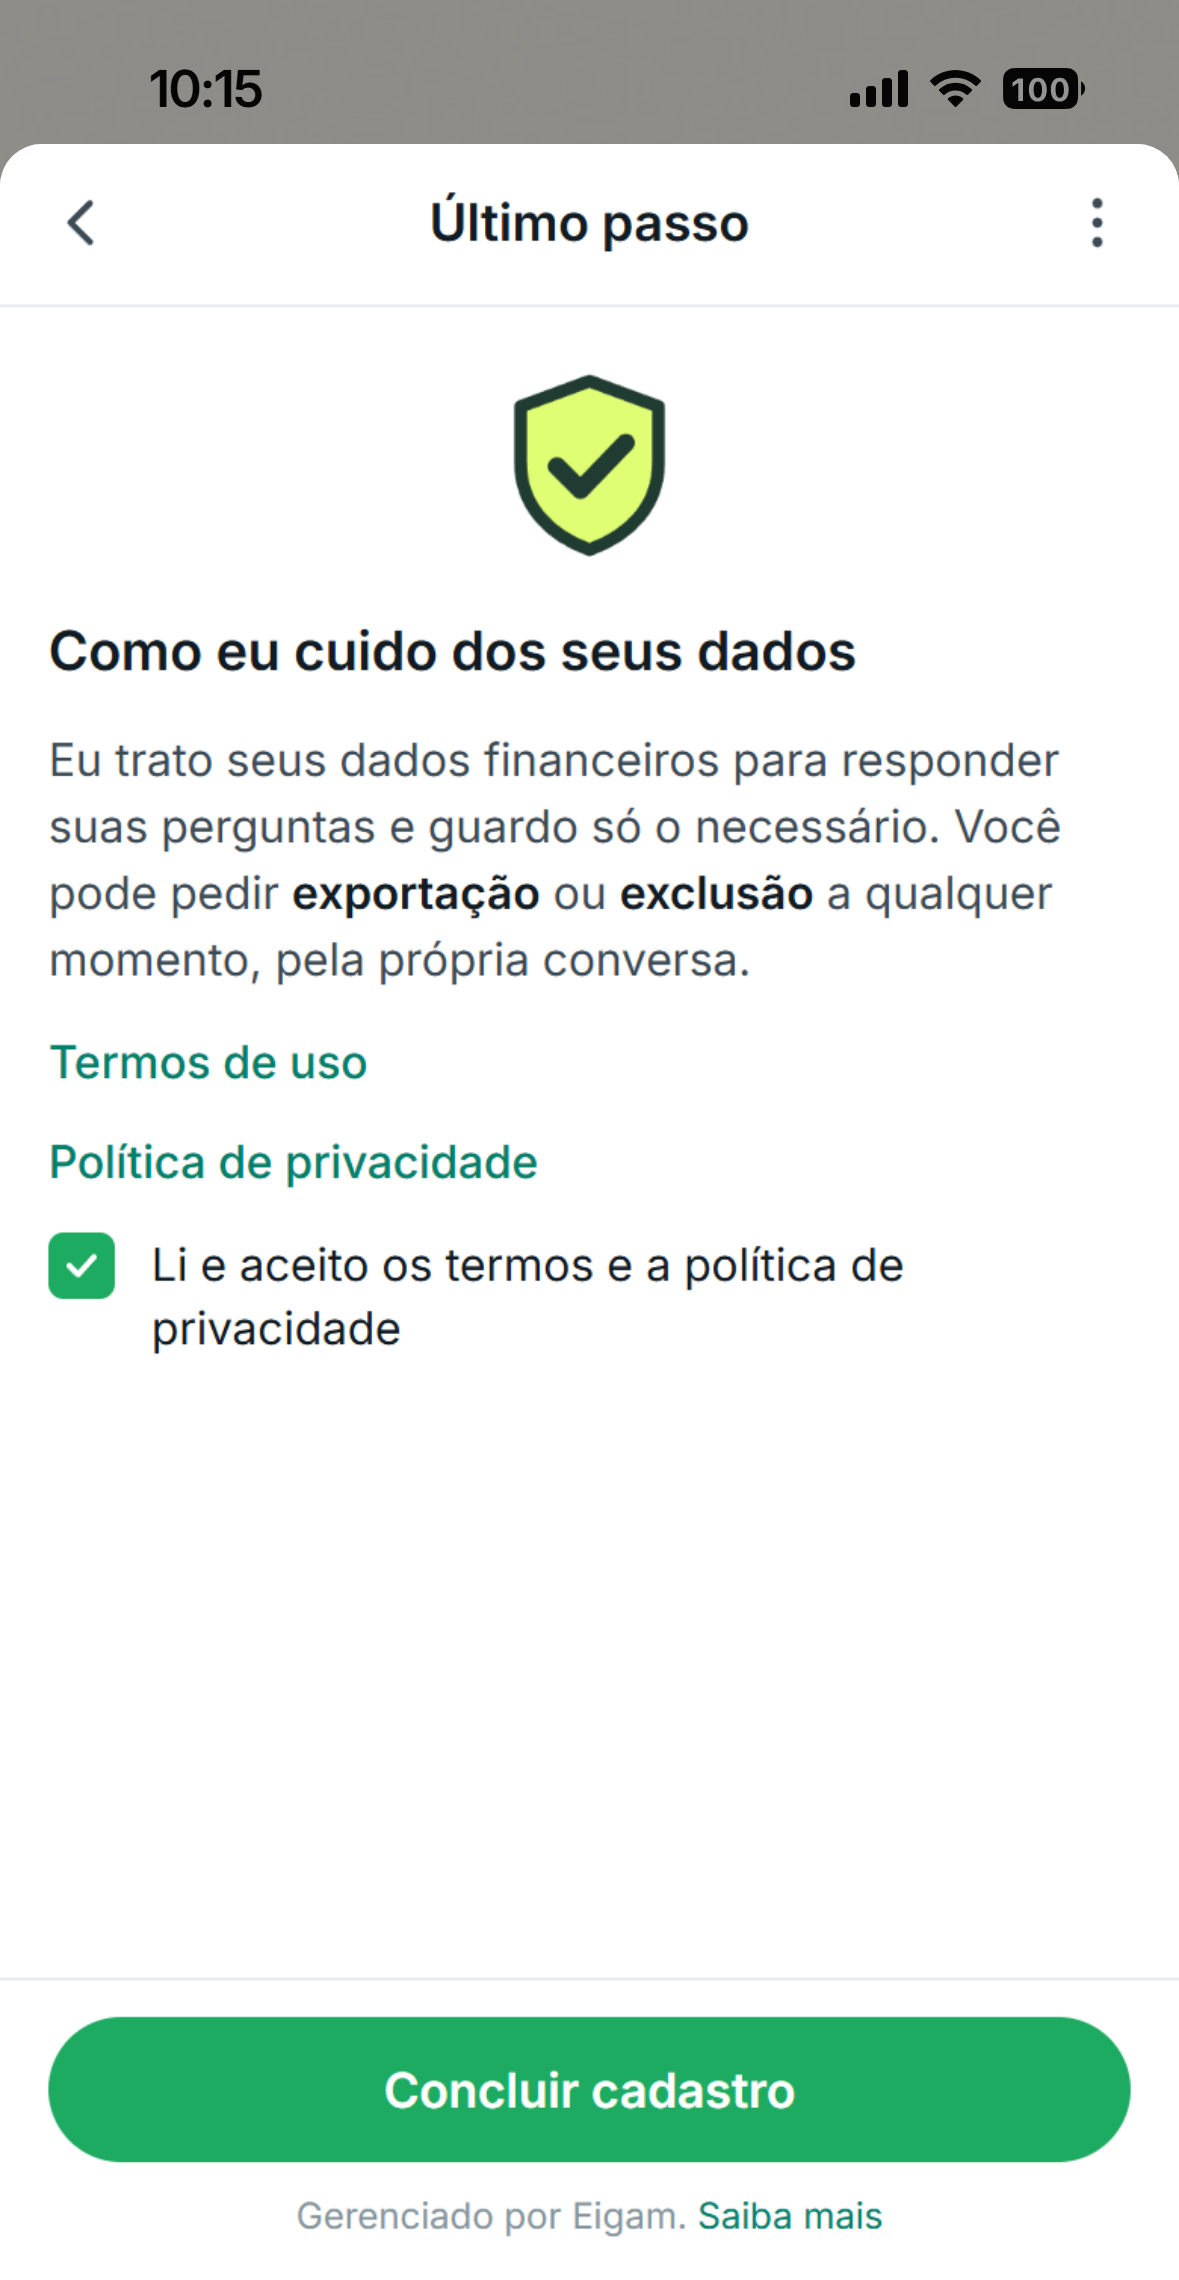
\includegraphics[width=\textwidth]{images/resultados/fluxos/form_cadastro_e.png}
    \end{minipage}\hfill
    \begin{minipage}[t]{0.32\textwidth}
        \centering
        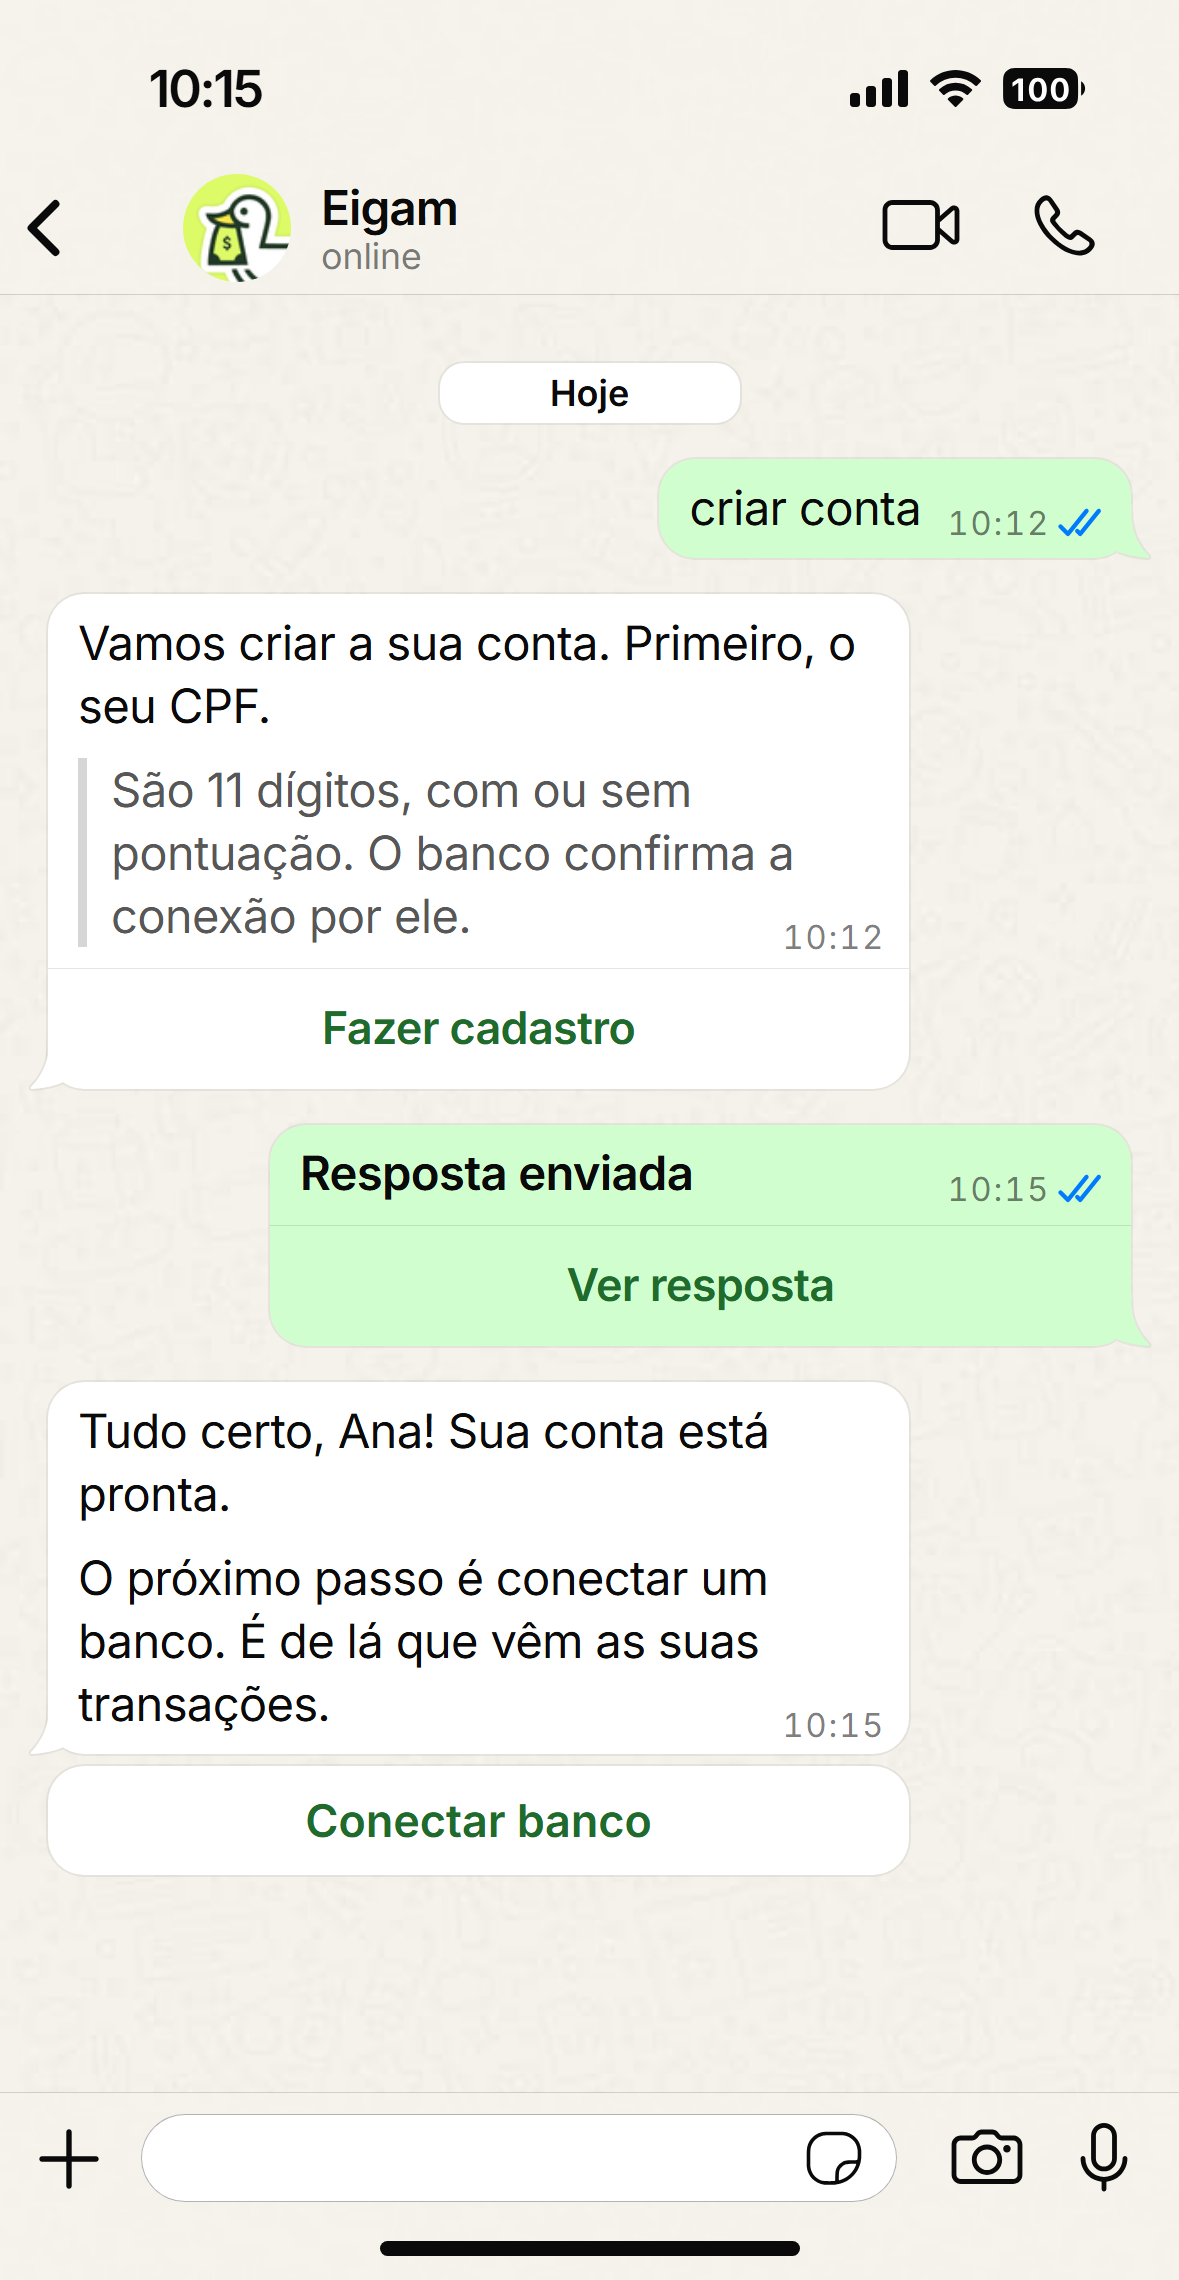
\includegraphics[width=\textwidth]{images/resultados/fluxos/form_cadastro_f.png}
    \end{minipage}
    \authorssource
\end{figure}

O cadastro (Figura~\ref{fig:form_cadastro}) começa com três compromissos (dados cifrados, valores só com o PIN e liberdade para exportar ou apagar tudo), segue com nome, CPF e e-mail, cria o PIN de seis dígitos e termina com o aceite dos termos. Ao enviar, a confirmação chega na conversa, já com o botão para conectar o primeiro banco. Antes disso, quem ainda não decidiu se cadastrar pode perguntar o que quiser sobre o produto e experimentar o assistente com uma base de demonstração, sem fornecer nenhum dado pessoal.

\begin{figure}[H]
    \centering
    \caption{Conexão de banco pelo formulário do \textit{WhatsApp Flows}}
    \label{fig:form_banco}
    \begin{minipage}[t]{0.32\textwidth}
        \centering
        
\includegraphics[width=\textwidth]{images/resultados/fluxos/form_banco_a.png}
    \end{minipage}\hfill
    \begin{minipage}[t]{0.32\textwidth}
        \centering
        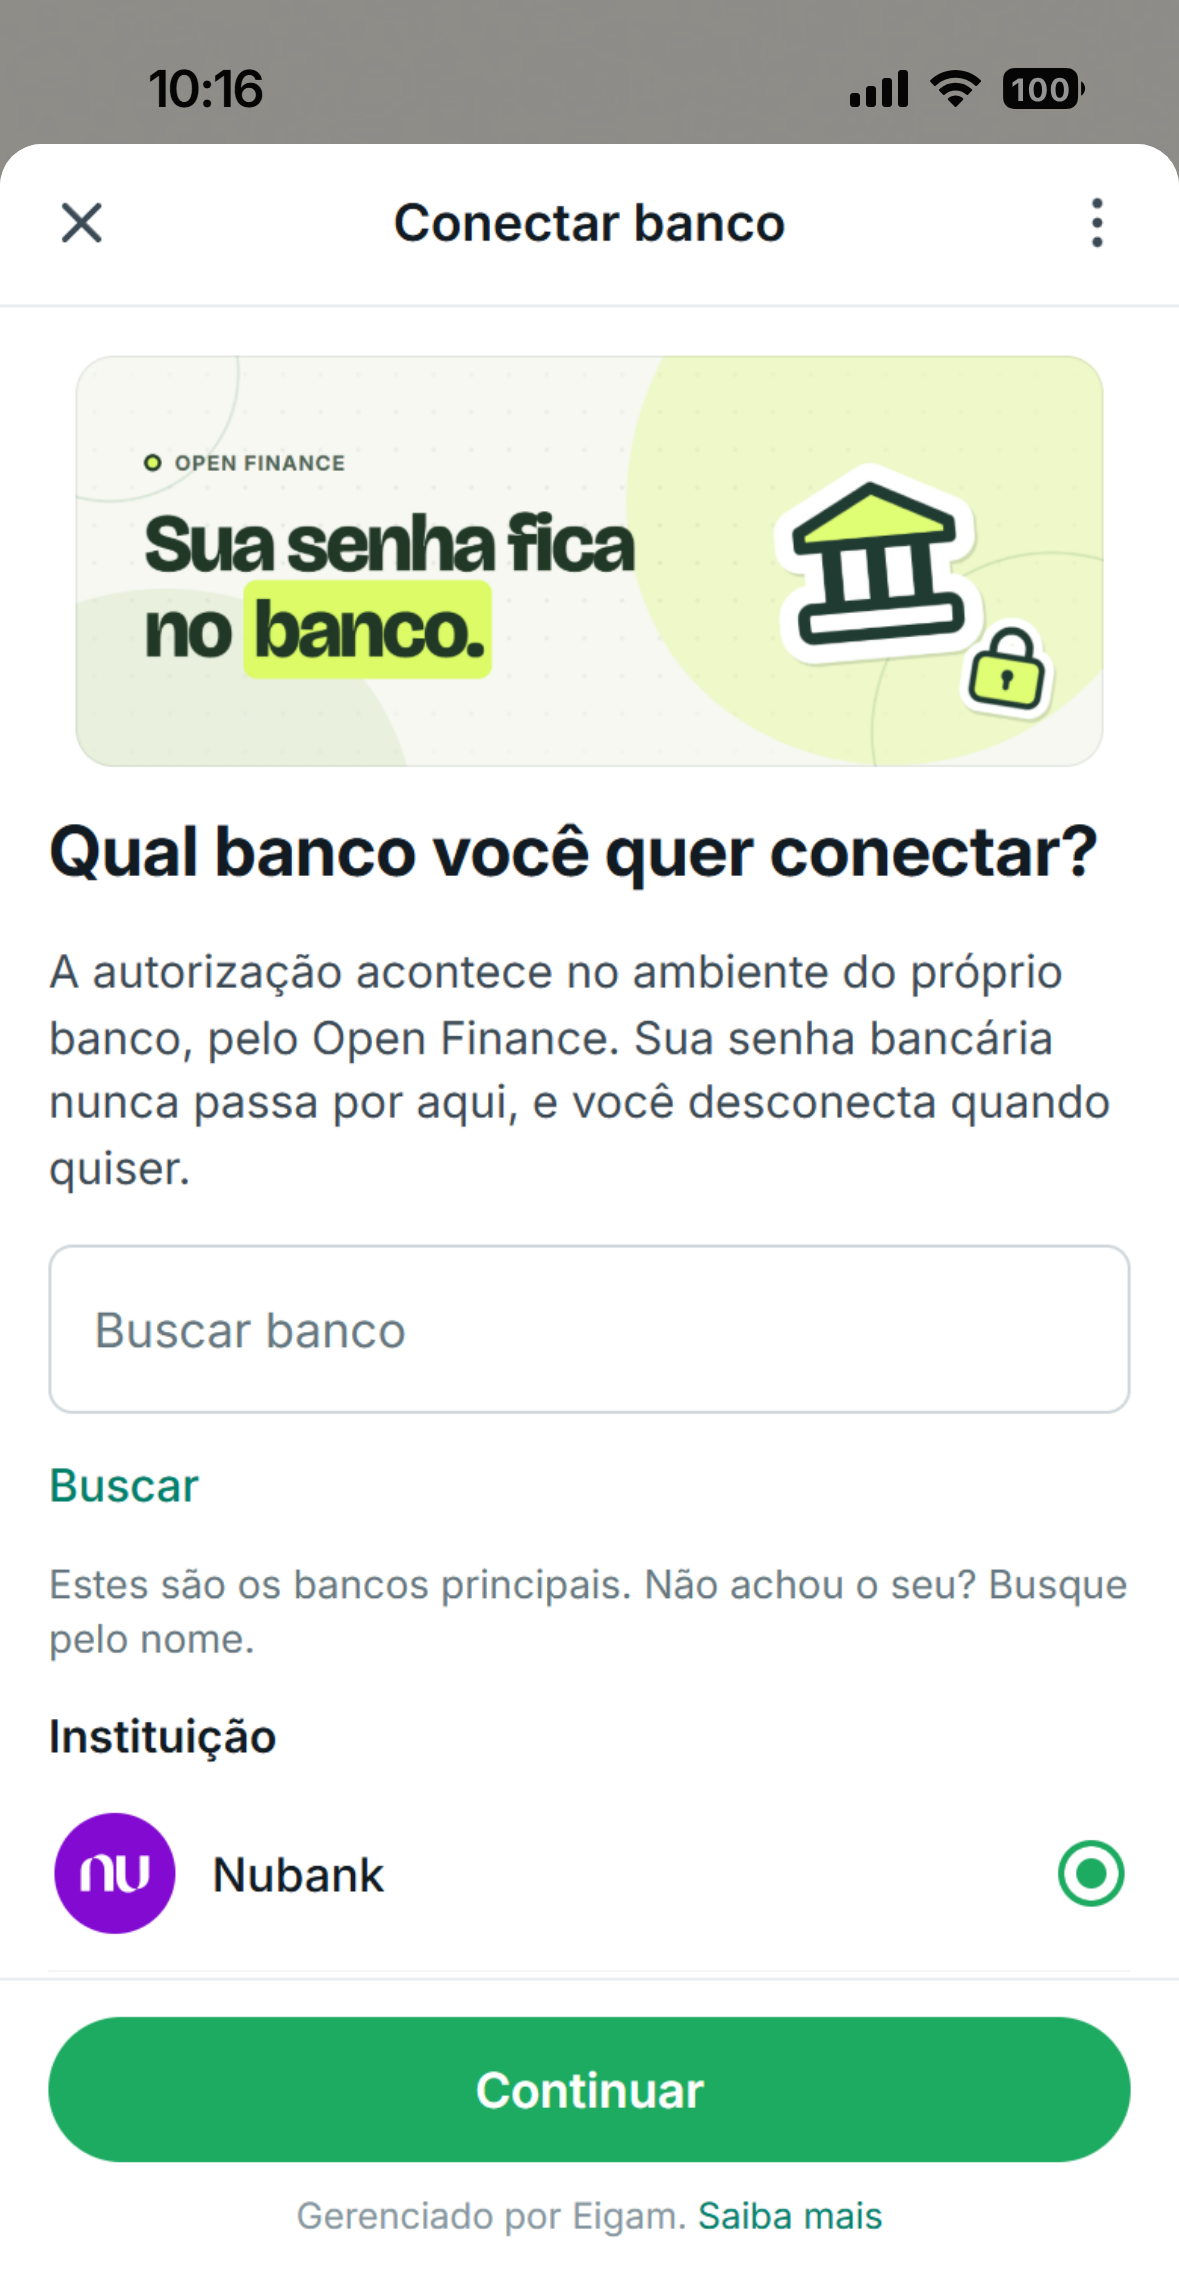
\includegraphics[width=\textwidth]{images/resultados/fluxos/form_banco_b.png}
    \end{minipage}\hfill
    \begin{minipage}[t]{0.32\textwidth}
        \centering
        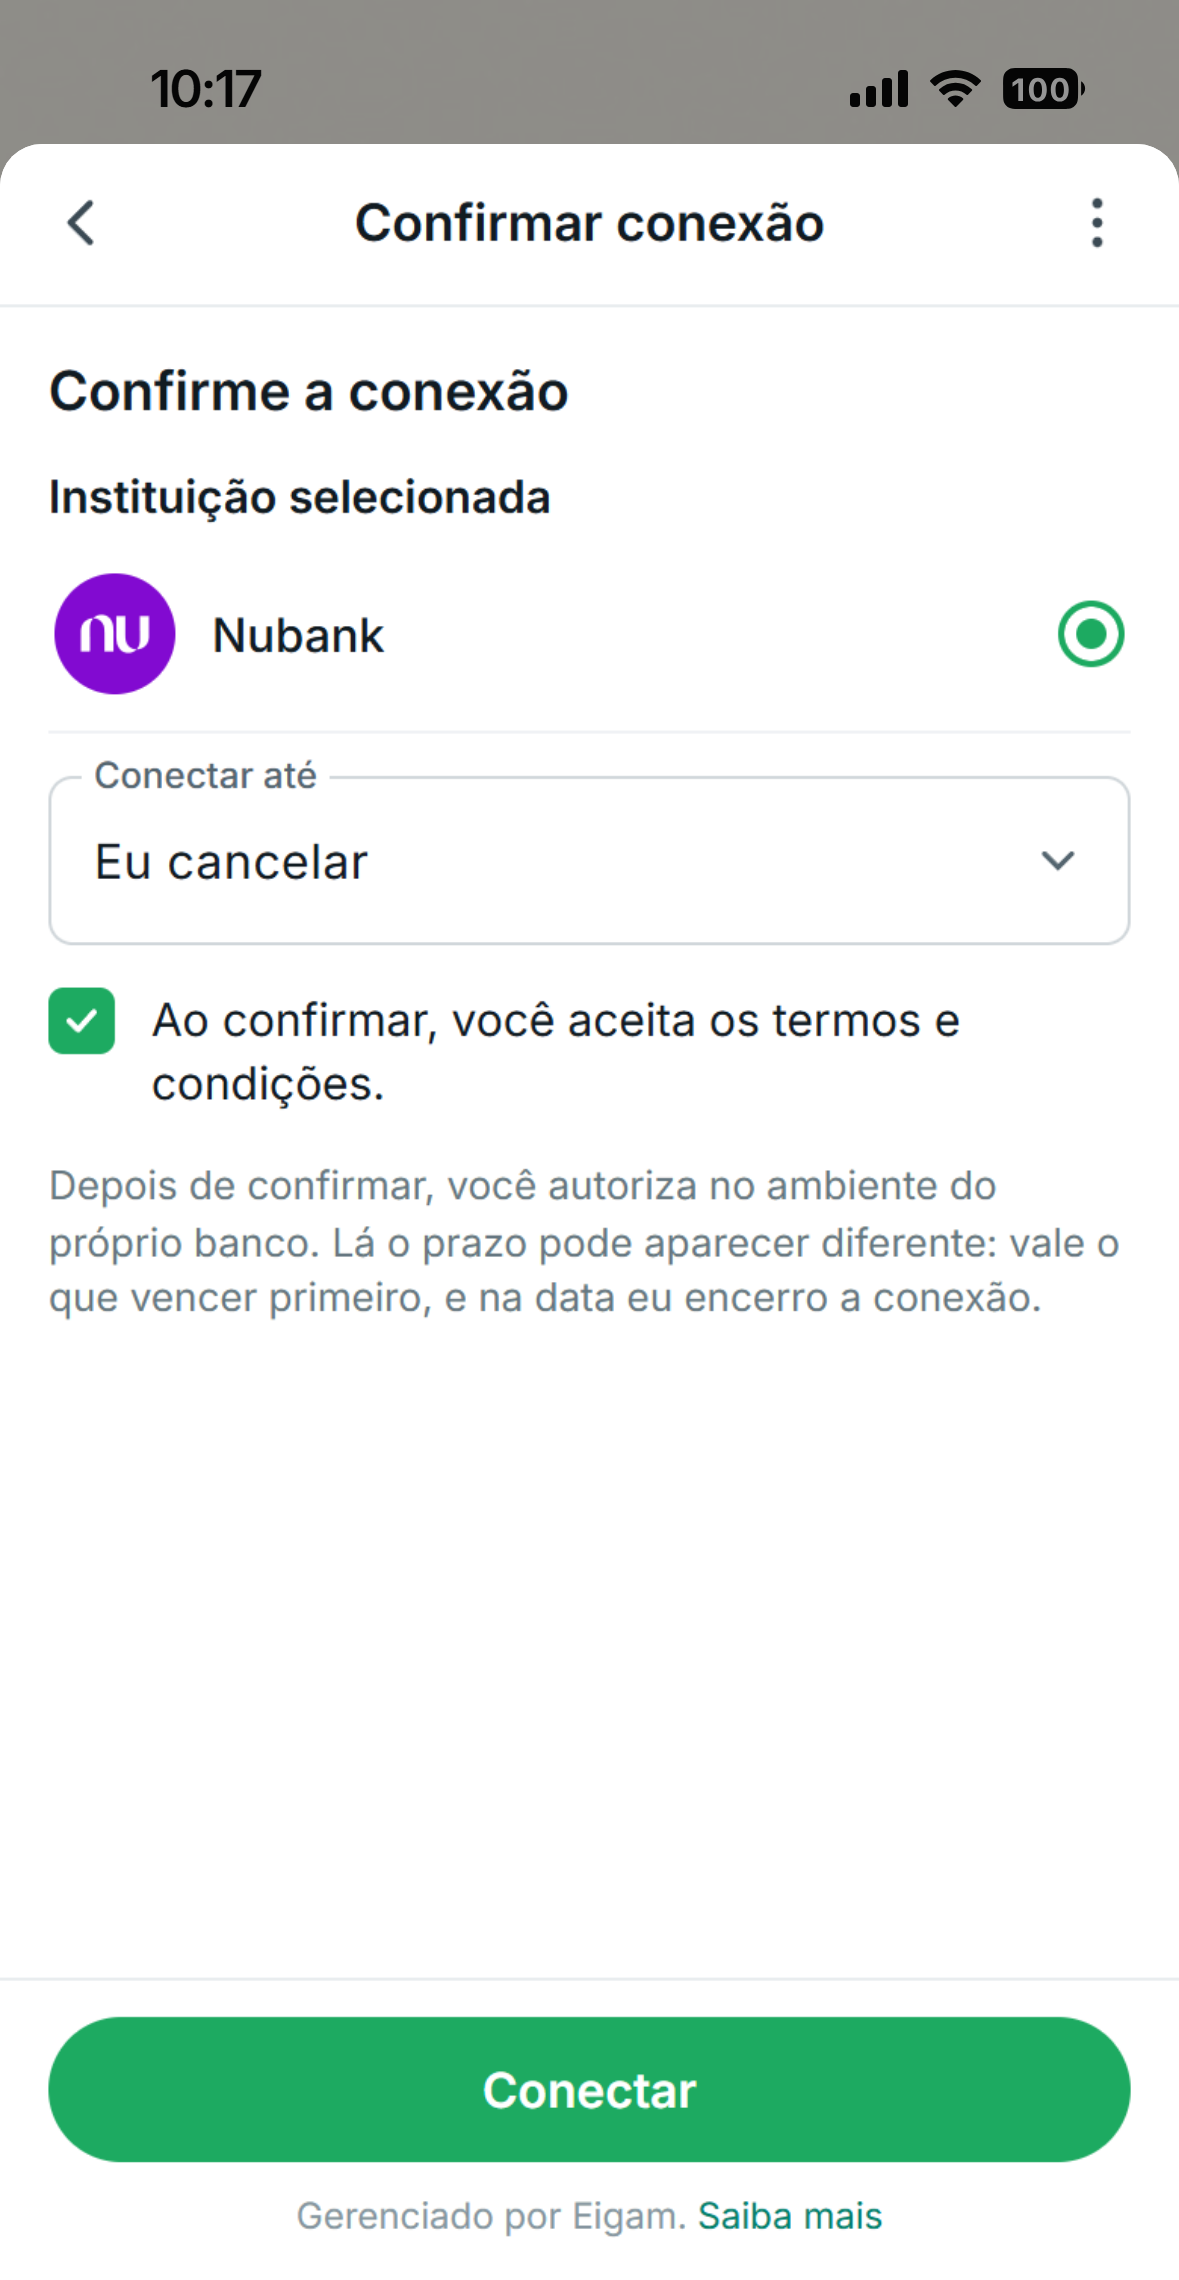
\includegraphics[width=\textwidth]{images/resultados/fluxos/form_banco_c.png}
    \end{minipage}
    \authorssource
\end{figure}

Na conexão de banco (Figura~\ref{fig:form_banco}), o titular escolhe a instituição e por quanto tempo o compartilhamento deve valer: três, seis ou doze meses, ou até cancelar. A autorização acontece no ambiente do próprio banco, pelo \textit{Open Finance}, de modo que a senha bancária nunca passa pelo EIGAM. Na data escolhida, uma varredura encerra a conexão no agregador e revoga o consentimento.

\begin{figure}[H]
    \centering
    \caption{Direitos do titular pelo formulário do \textit{WhatsApp Flows}}
    \label{fig:form_direitos}
    \begin{minipage}[t]{0.32\textwidth}
        \centering
        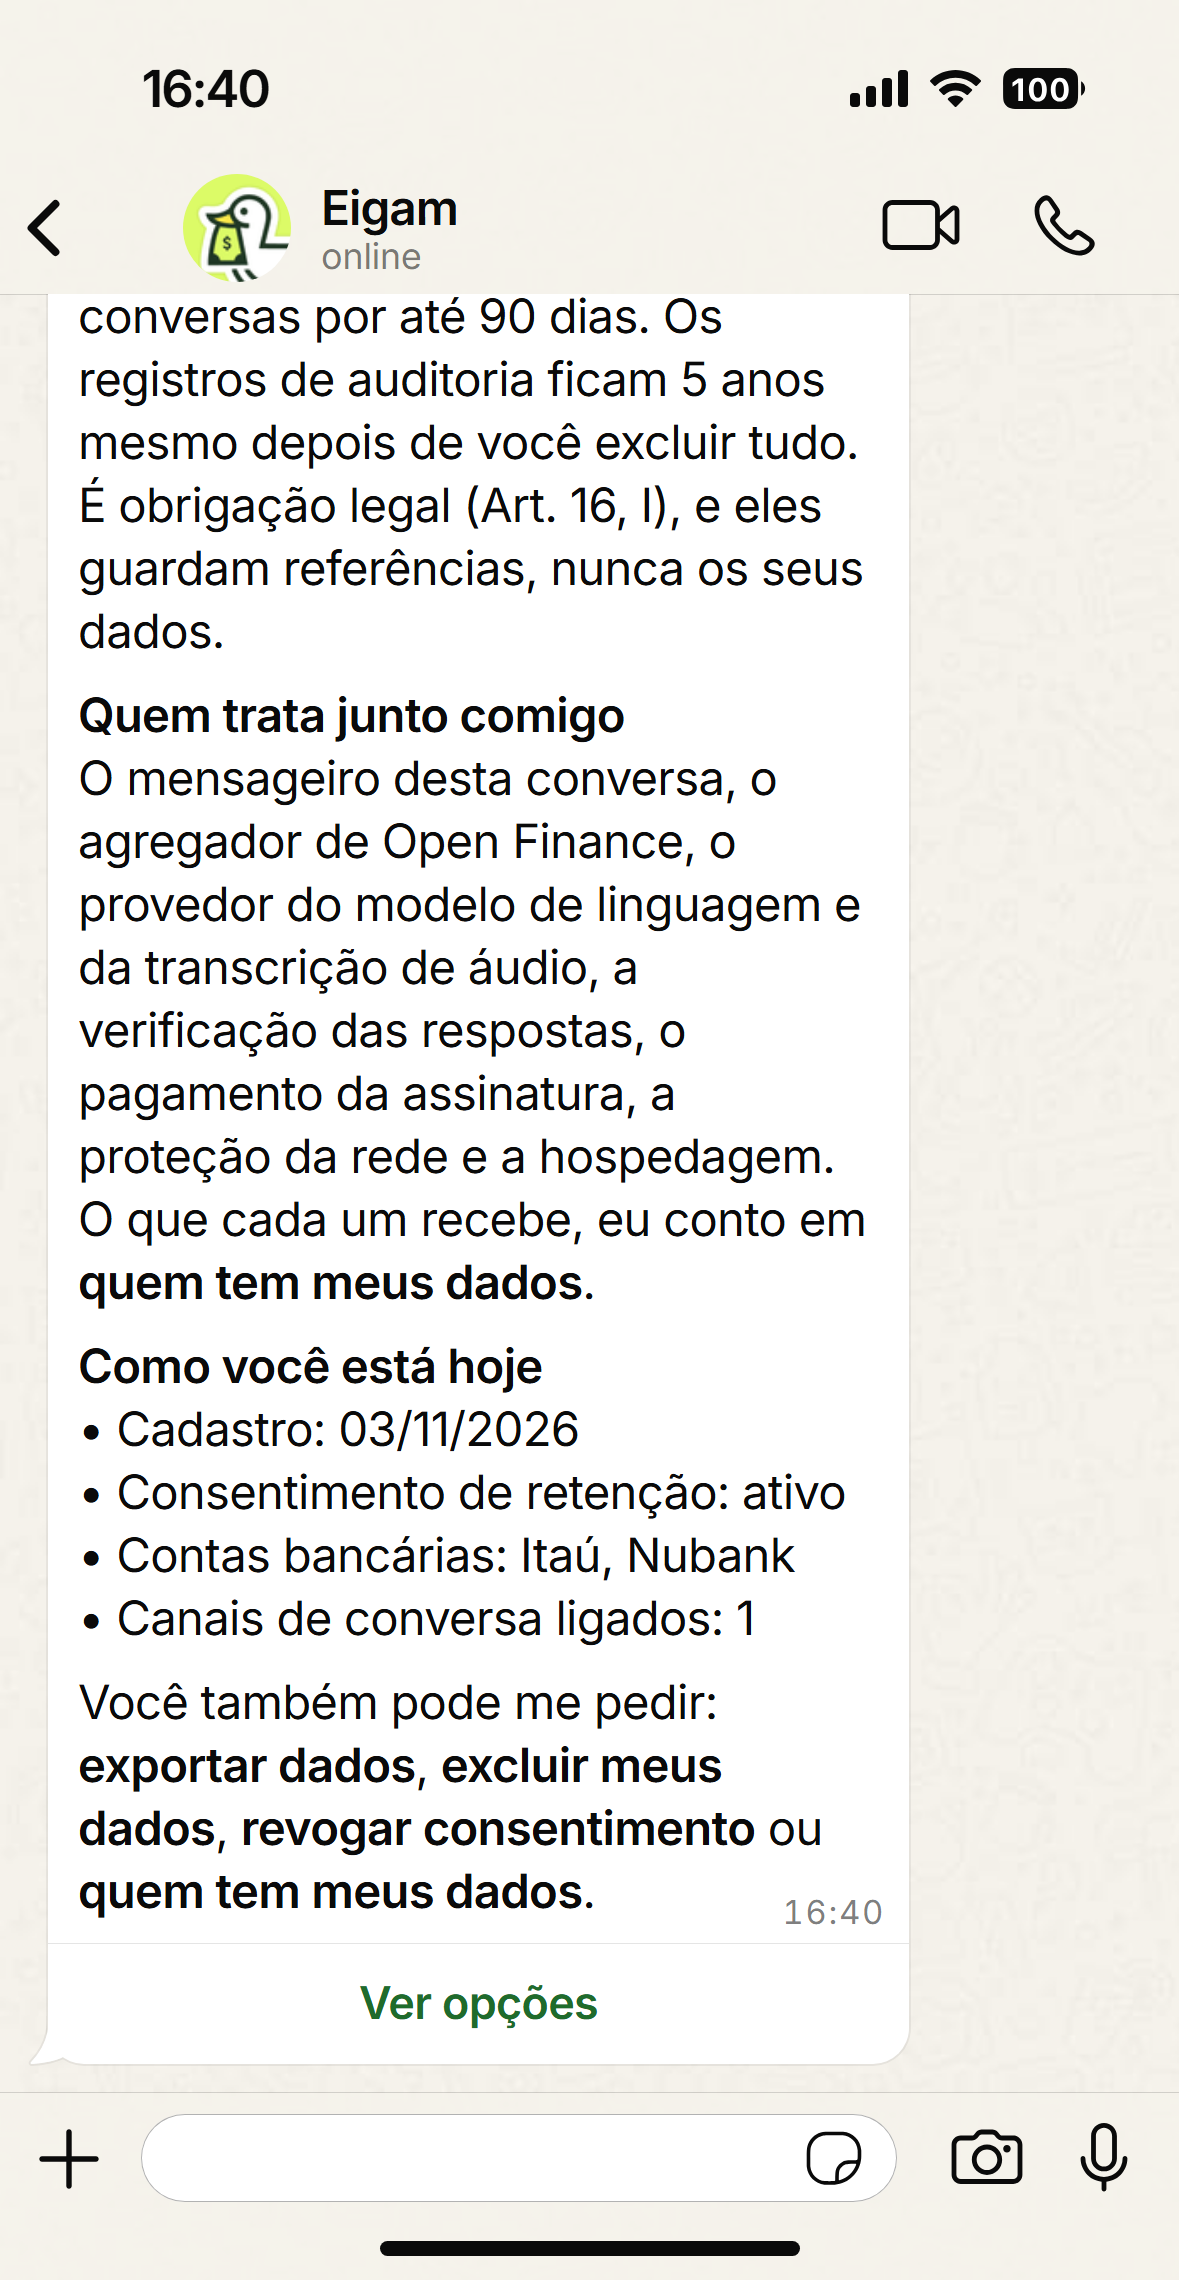
\includegraphics[width=\textwidth]{images/resultados/fluxos/form_direitos_a.png}
    \end{minipage}\hfill
    \begin{minipage}[t]{0.32\textwidth}
        \centering
        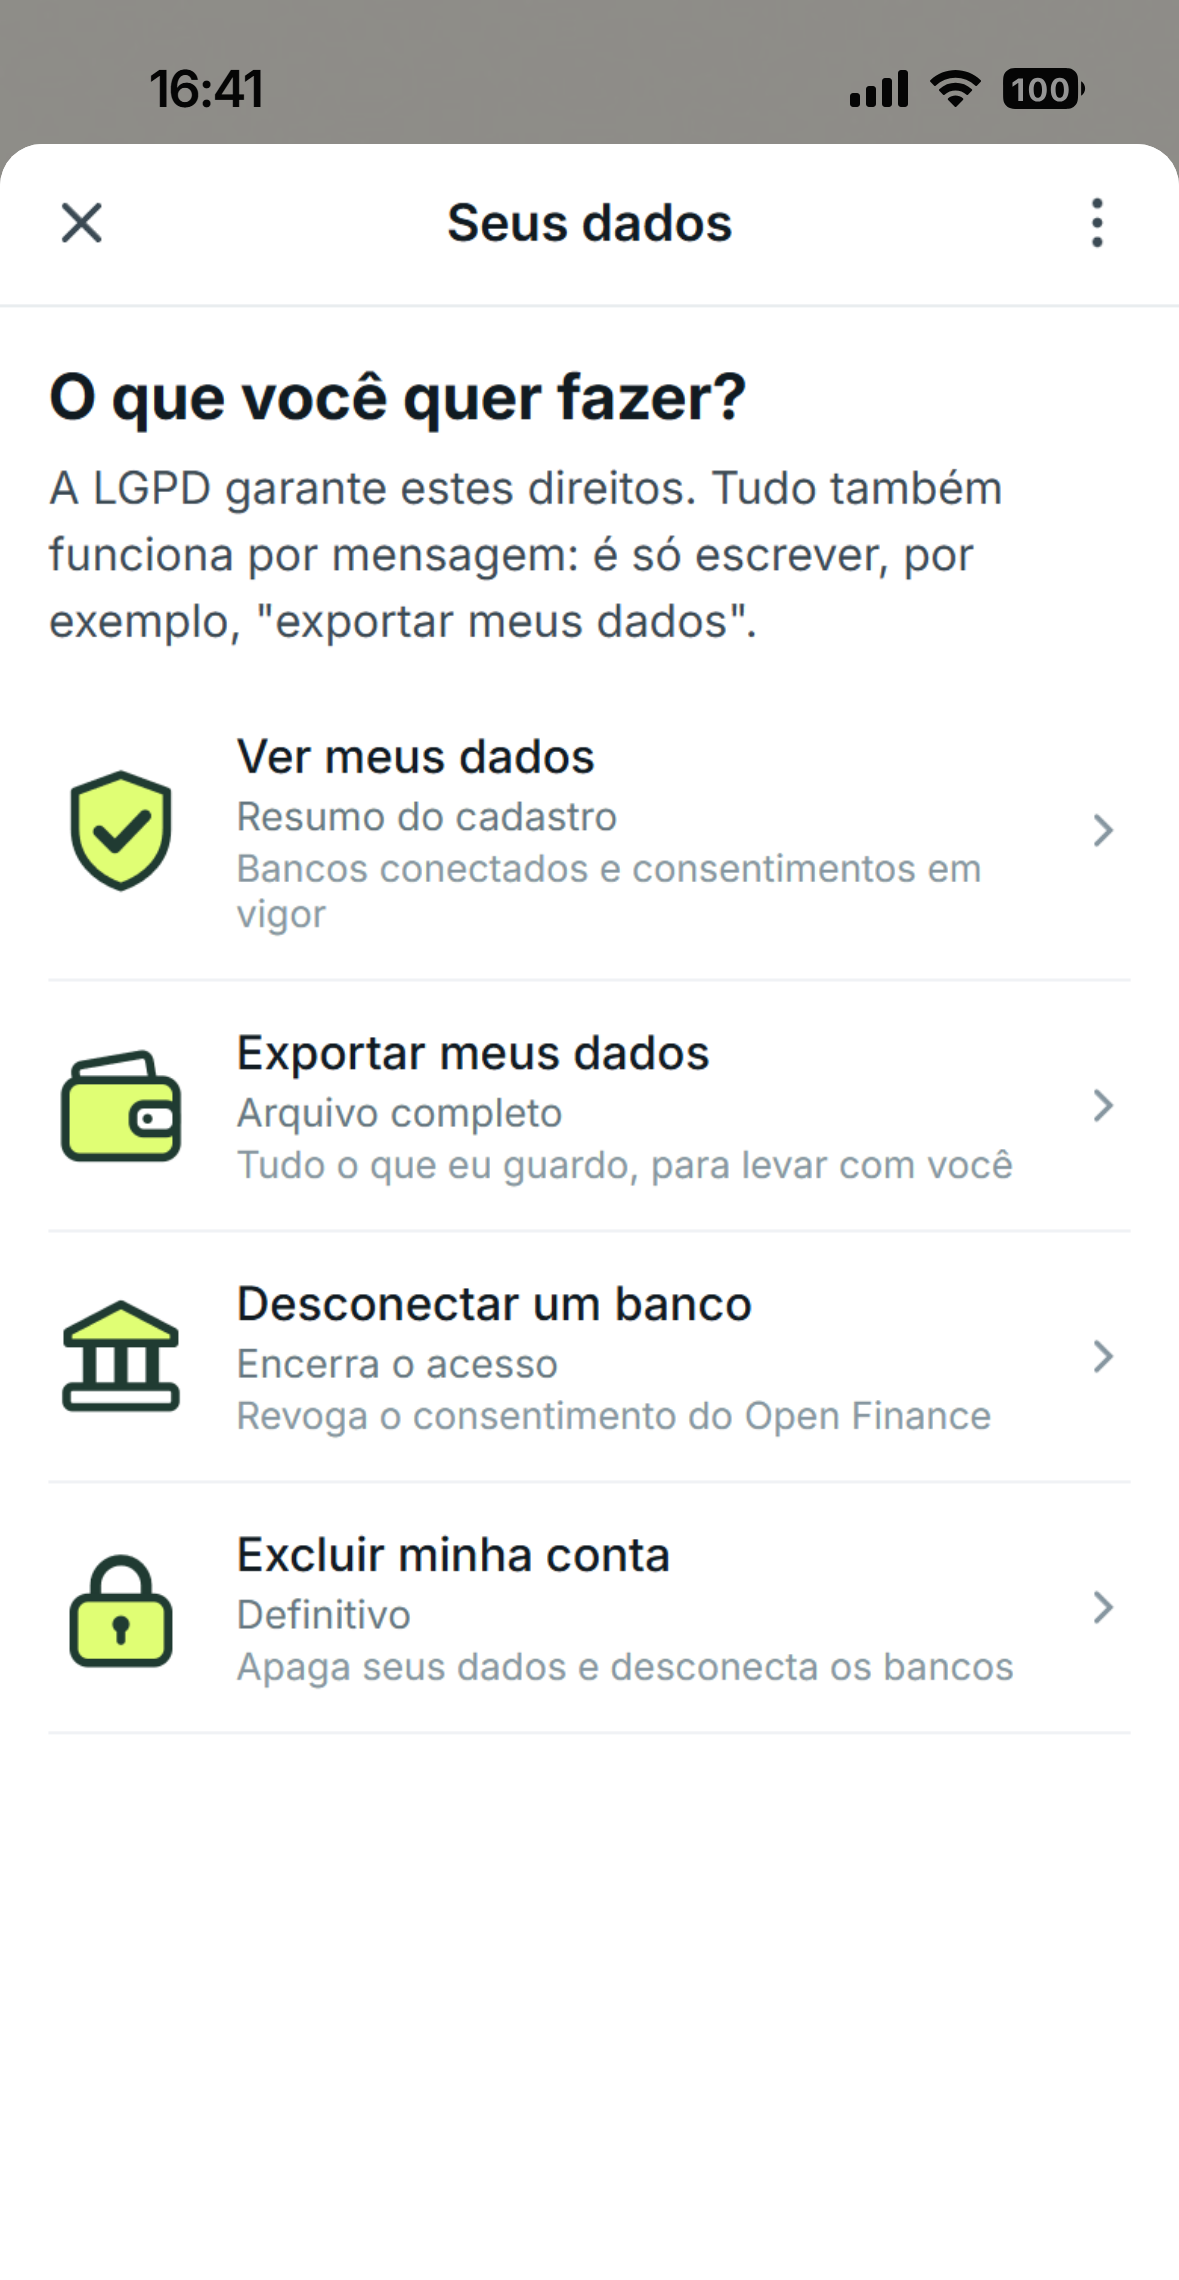
\includegraphics[width=\textwidth]{images/resultados/fluxos/form_direitos_b.png}
    \end{minipage}\hfill
    \begin{minipage}[t]{0.32\textwidth}
        \centering
        
\includegraphics[width=\textwidth]{images/resultados/fluxos/form_direitos_c.png}
    \end{minipage}
    \authorssource
\end{figure}

\begin{figure}[H]
    \centering
    \caption{Preferências de aviso pelo formulário do \textit{WhatsApp Flows}}
    \label{fig:form_preferencias}
    \begin{minipage}[t]{0.32\textwidth}
        \centering
        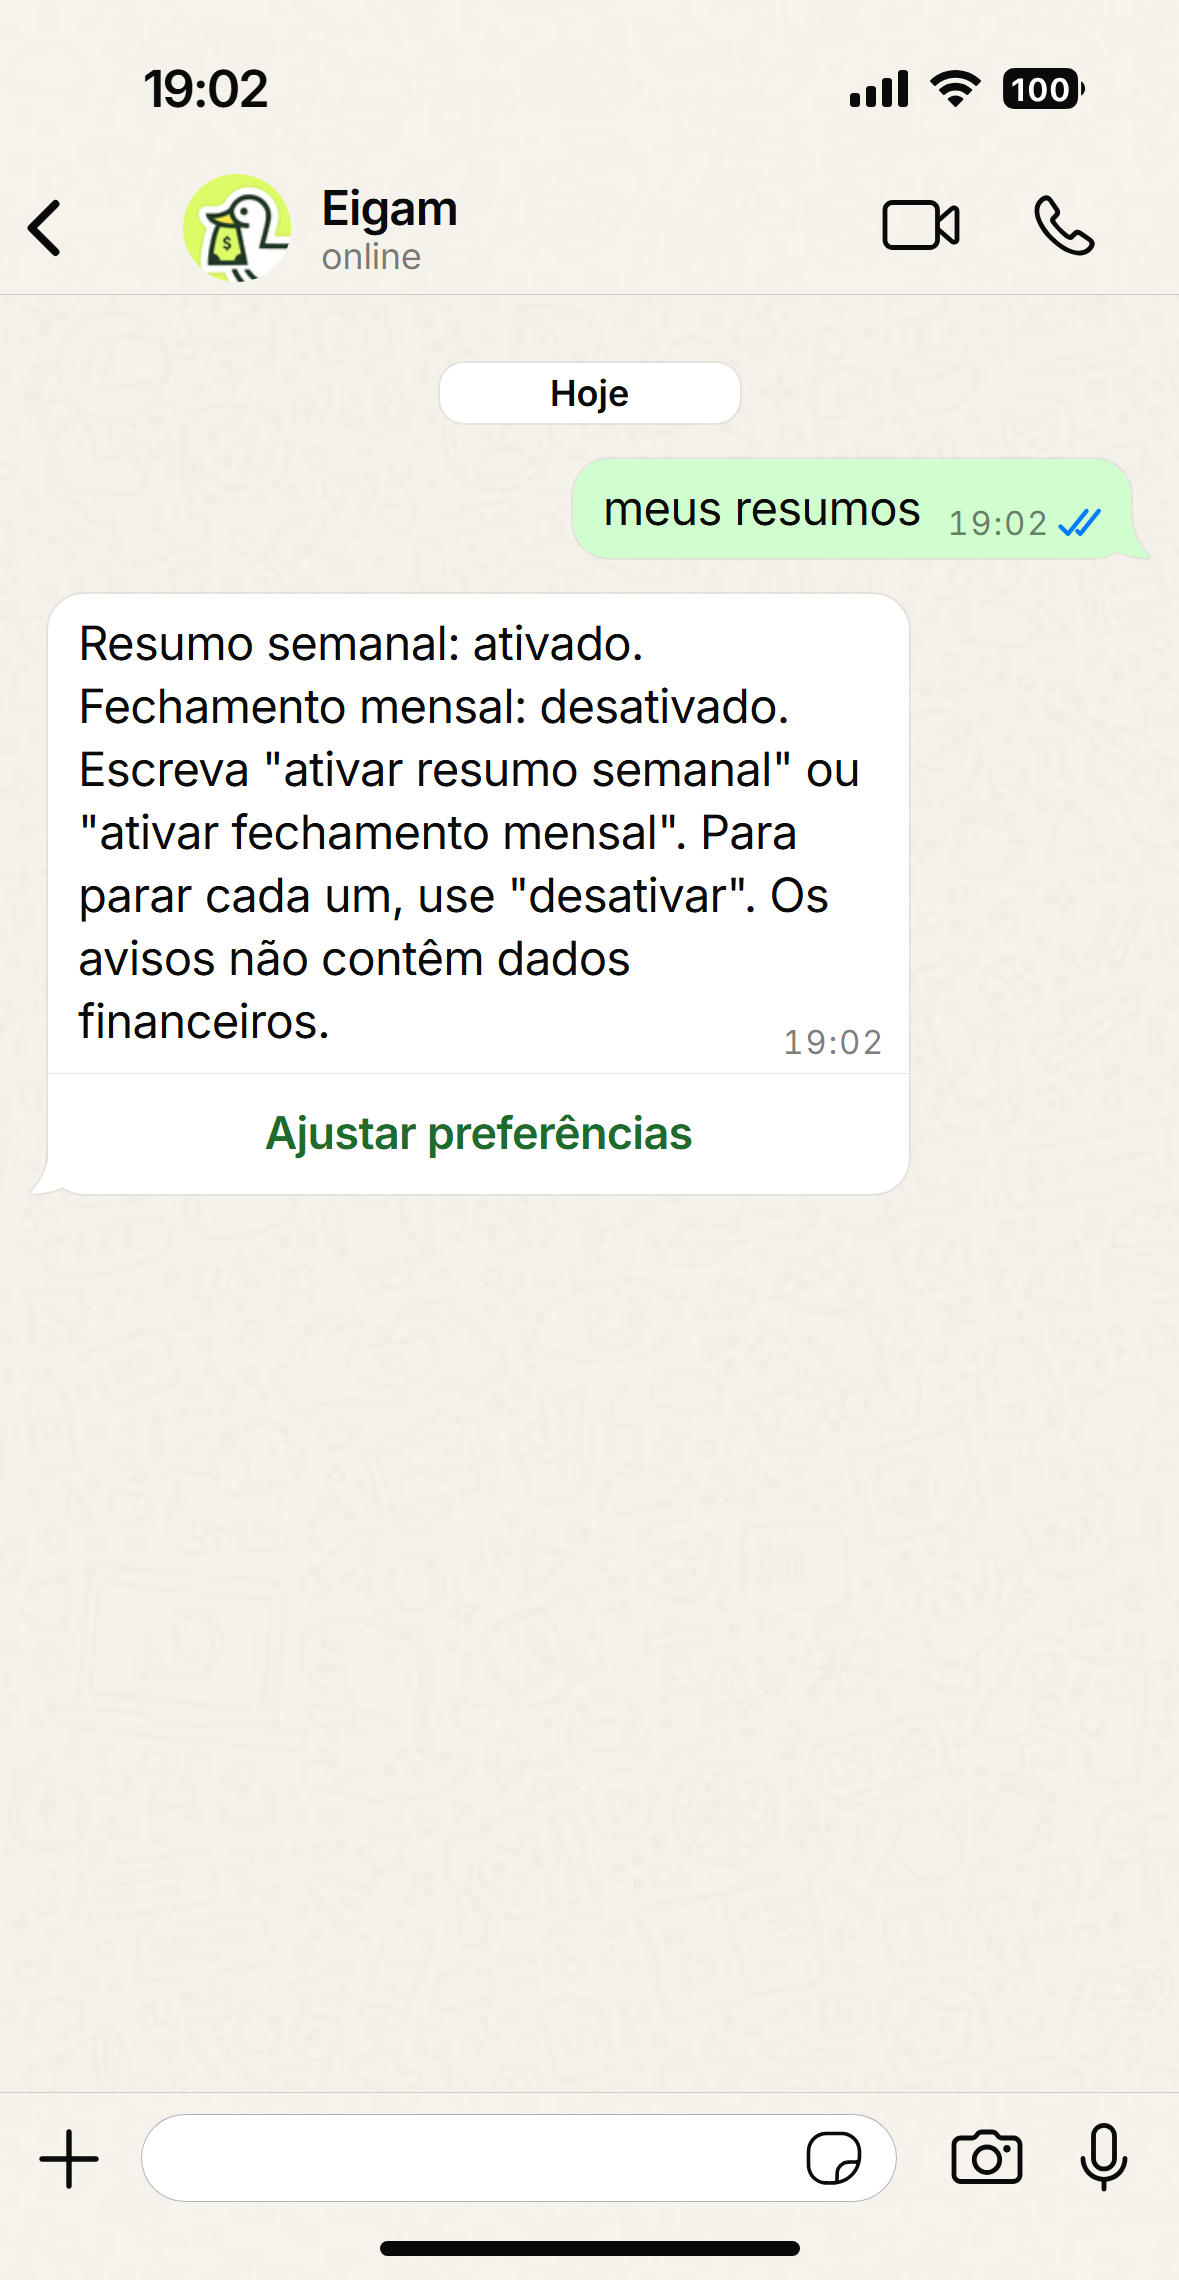
\includegraphics[width=\textwidth]{images/resultados/fluxos/form_preferencias_a.png}
    \end{minipage}\hfill
    \begin{minipage}[t]{0.32\textwidth}
        \centering
        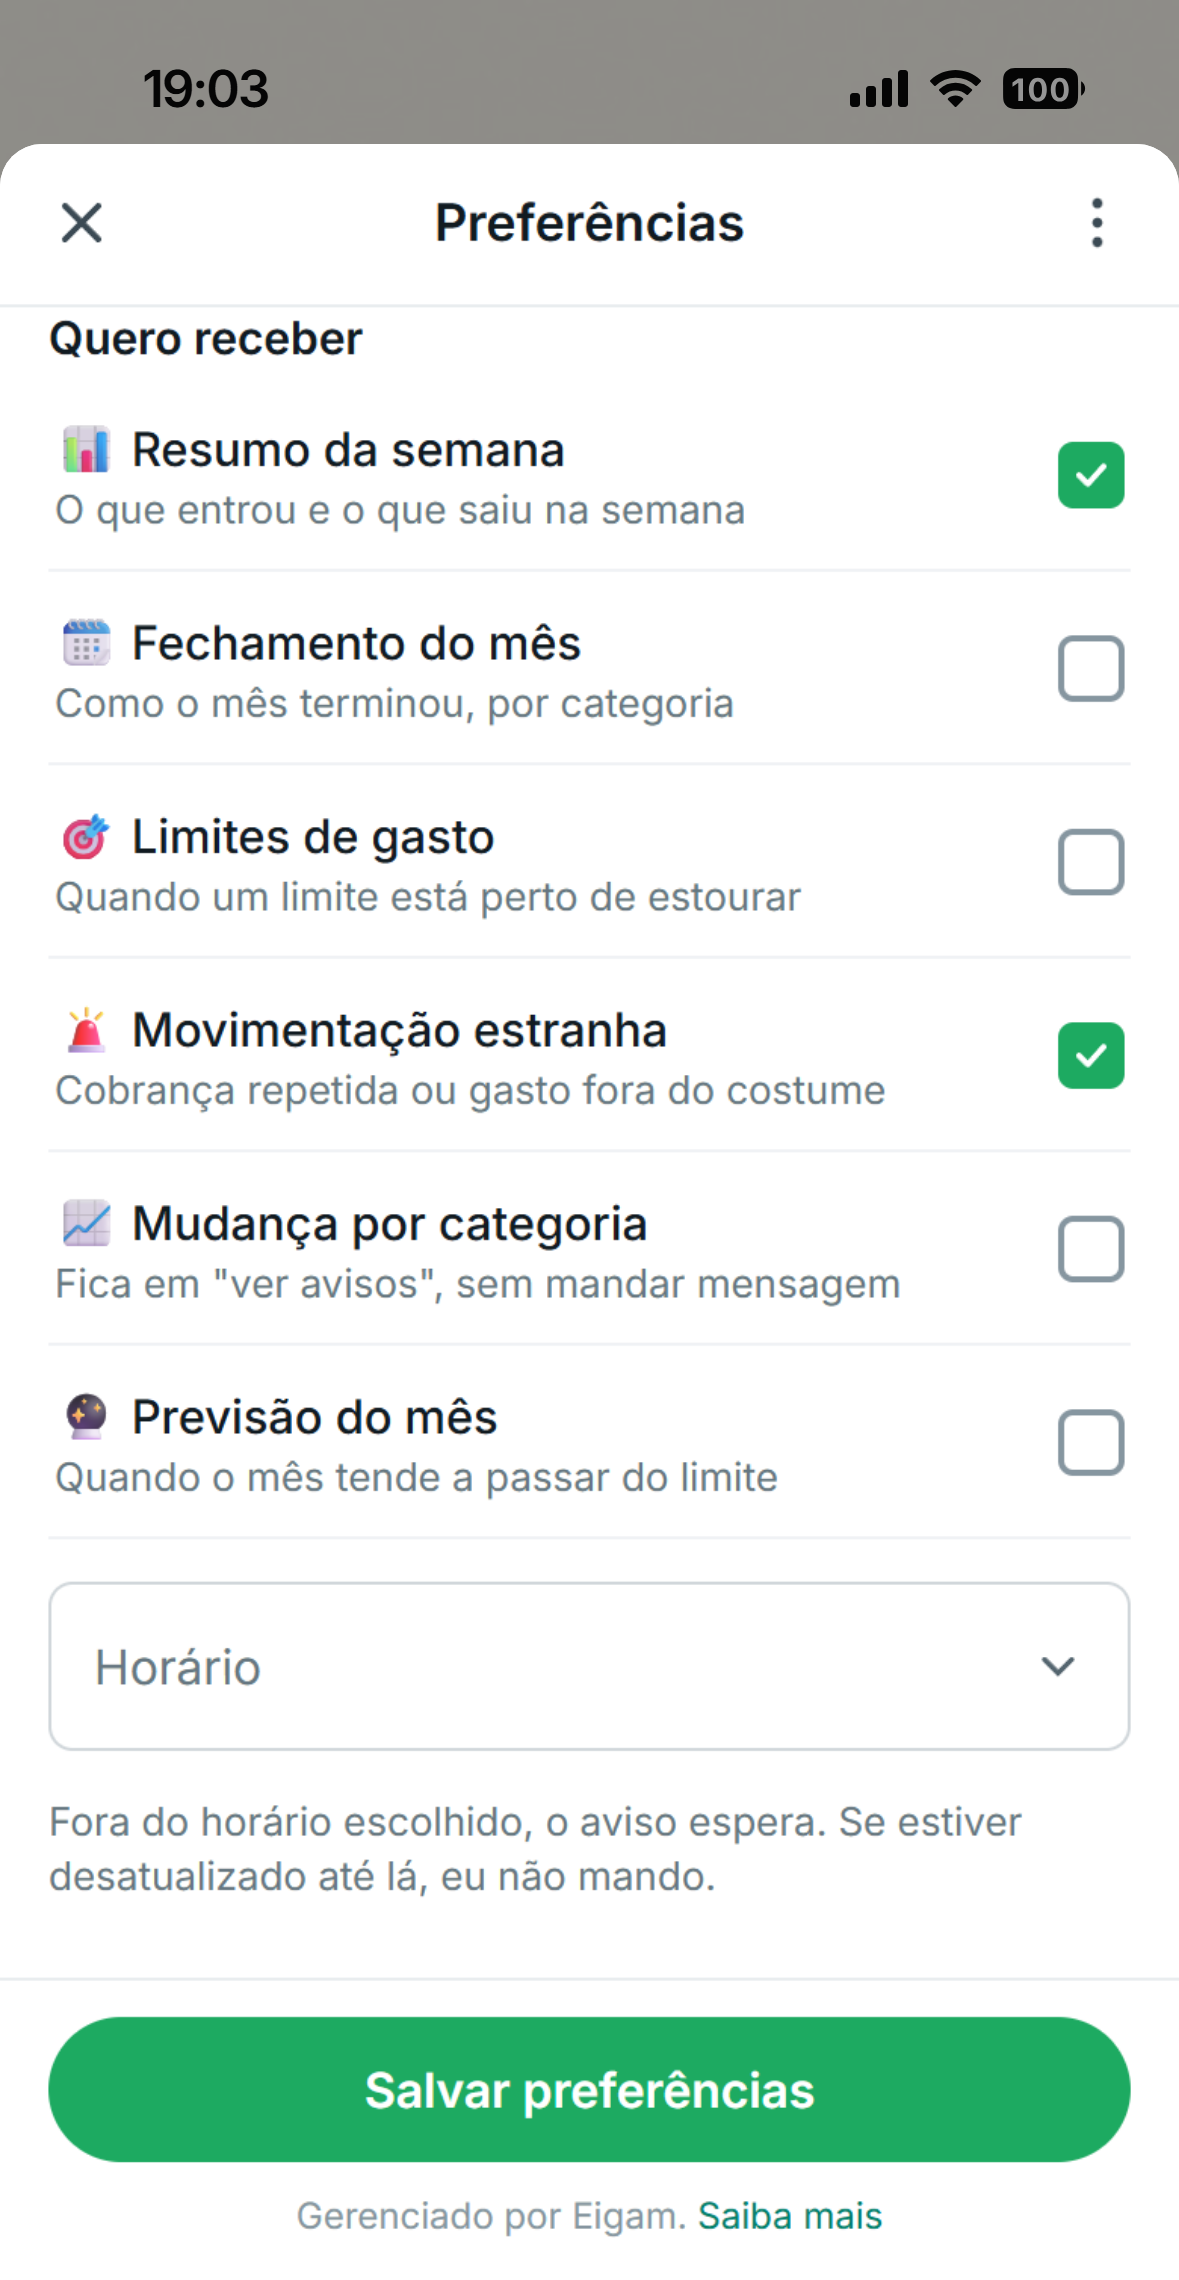
\includegraphics[width=\textwidth]{images/resultados/fluxos/form_preferencias_b.png}
    \end{minipage}\hfill
    \begin{minipage}[t]{0.32\textwidth}
        \centering
        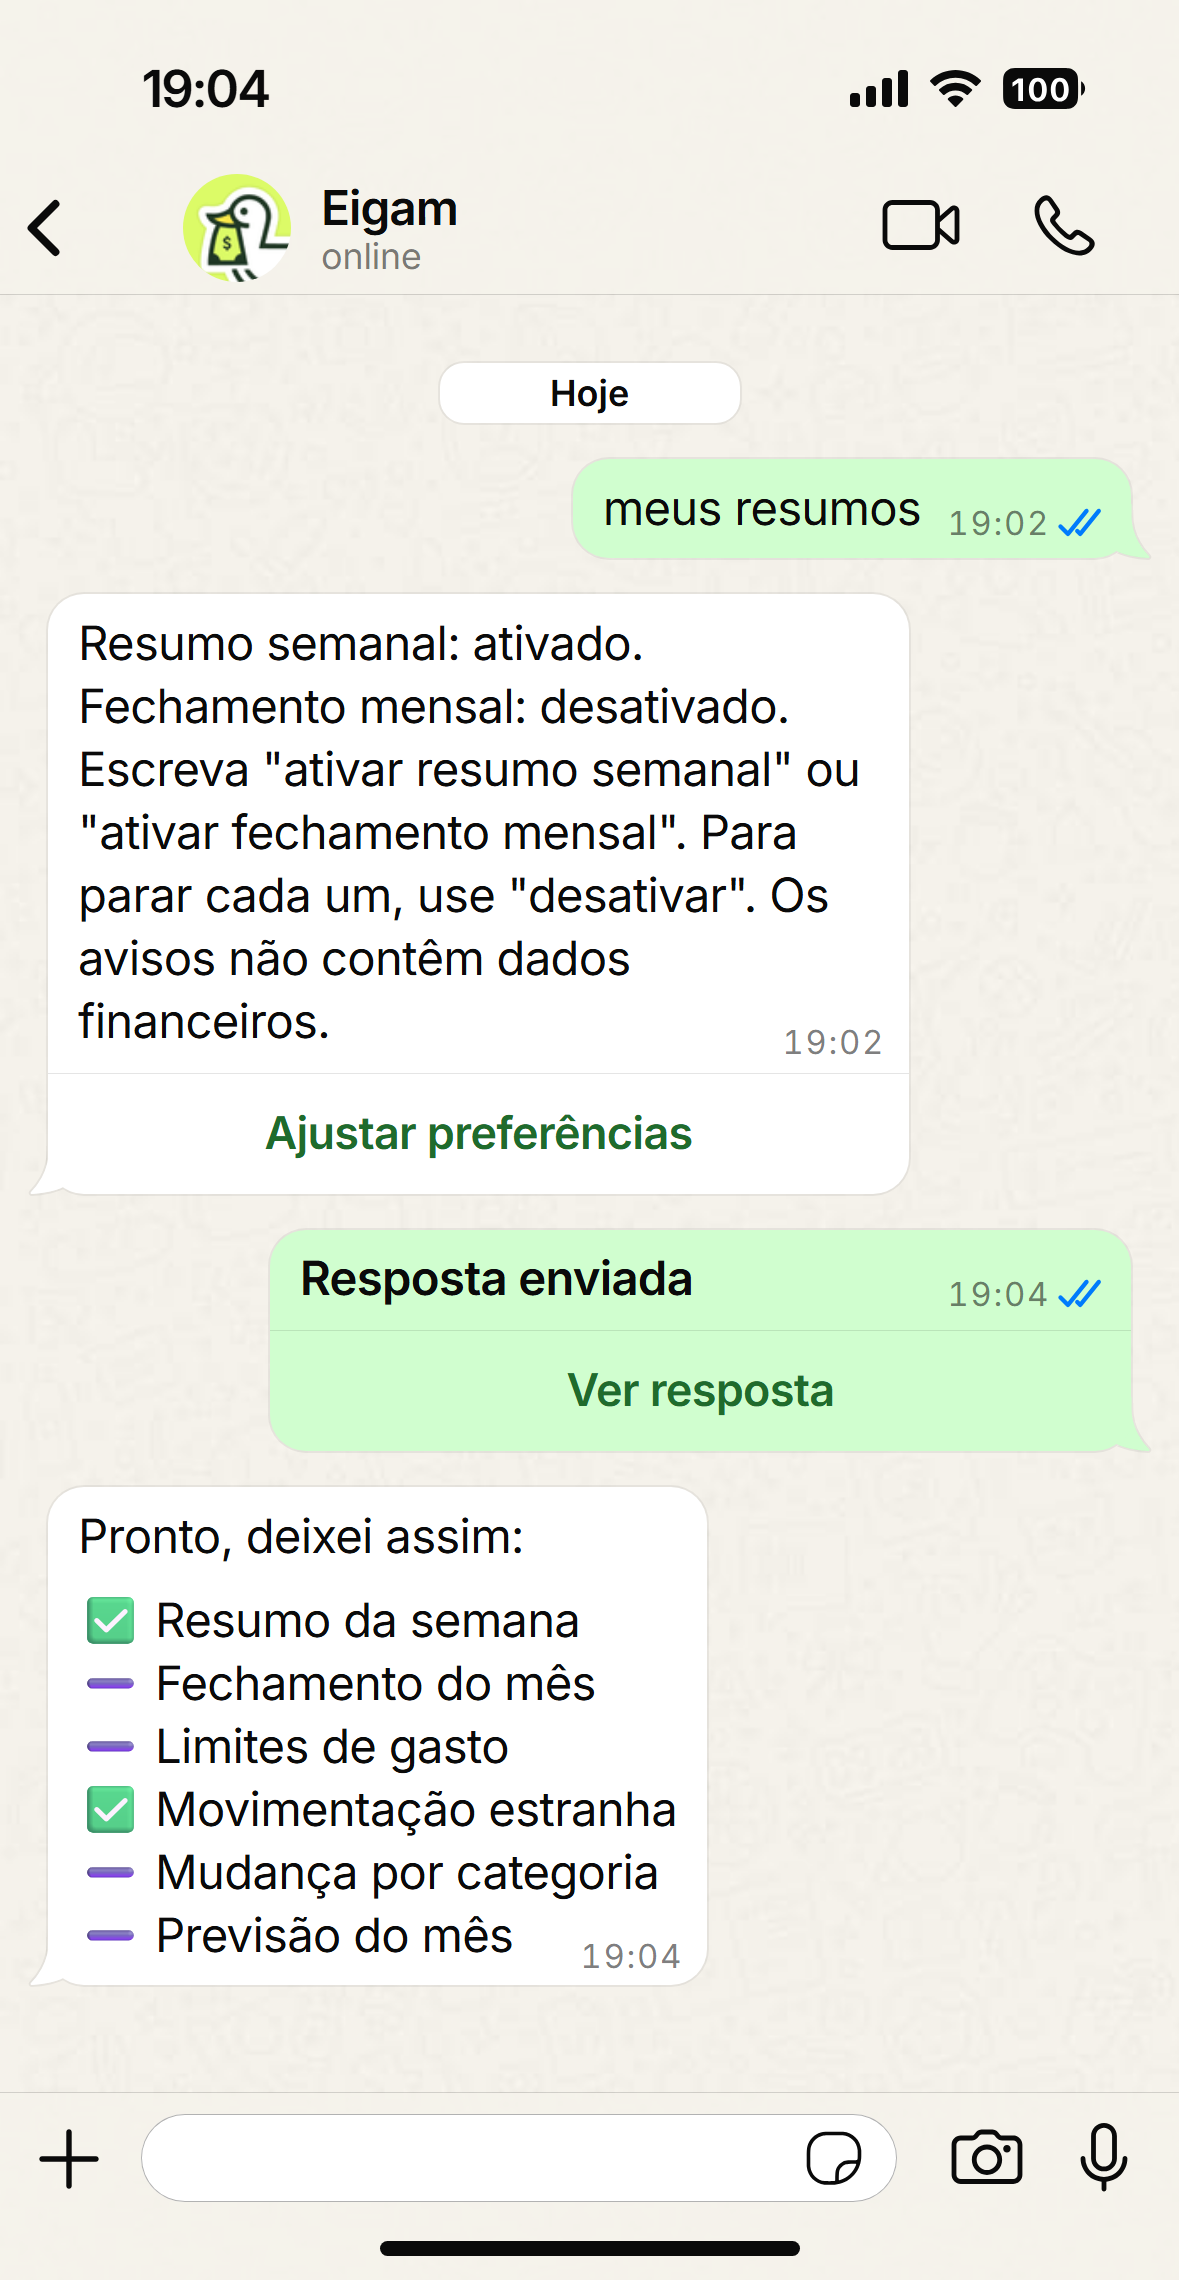
\includegraphics[width=\textwidth]{images/resultados/fluxos/form_preferencias_c.png}
    \end{minipage}
    \authorssource
\end{figure}

Os direitos da LGPD (Figura~\ref{fig:form_direitos}) podem ser exercidos pelo formulário, oferecido junto com o resumo do que é tratado sobre o titular, ou escrevendo o pedido na conversa, por exemplo ``exportar meus dados''. Os dois caminhos chegam ao mesmo reconhecimento determinístico e à mesma confirmação. Nas preferências (Figura~\ref{fig:form_preferencias}), o titular escolhe quais famílias de aviso quer receber e em qual faixa de horário; fora dela, o aviso espera e, se deixar de valer, não é enviado. Ao salvar, a conversa confirma a escolha item a item.

A Figura~\ref{fig:fluxo_flows} mostra o mesmo mecanismo em uma troca de PIN do beta. A conversa ofereceu o formulário com a justificativa de que, por ele, o PIN não fica no histórico da conversa; a folha nativa abre sobre o diálogo com os campos definidos uma única vez no \textit{gateway} (PIN atual, novo PIN e repetição) e, ao enviar, a confirmação voltou para a conversa. Como a troca encerra a liberação de valores que estava ativa, a pergunta seguinte sobre gastos já recebeu o valor oculto, com o pedido do novo PIN.

\begin{figure}[H]
    \centering
    \caption{Troca de PIN pelo formulário do \textit{WhatsApp Flows}}
    \label{fig:fluxo_flows}
    \begin{minipage}[t]{0.32\textwidth}
        \centering
        
\includegraphics[width=\textwidth]{images/resultados/fluxos/fluxo_flows_a.png}
    \end{minipage}\hfill
    \begin{minipage}[t]{0.32\textwidth}
        \centering
        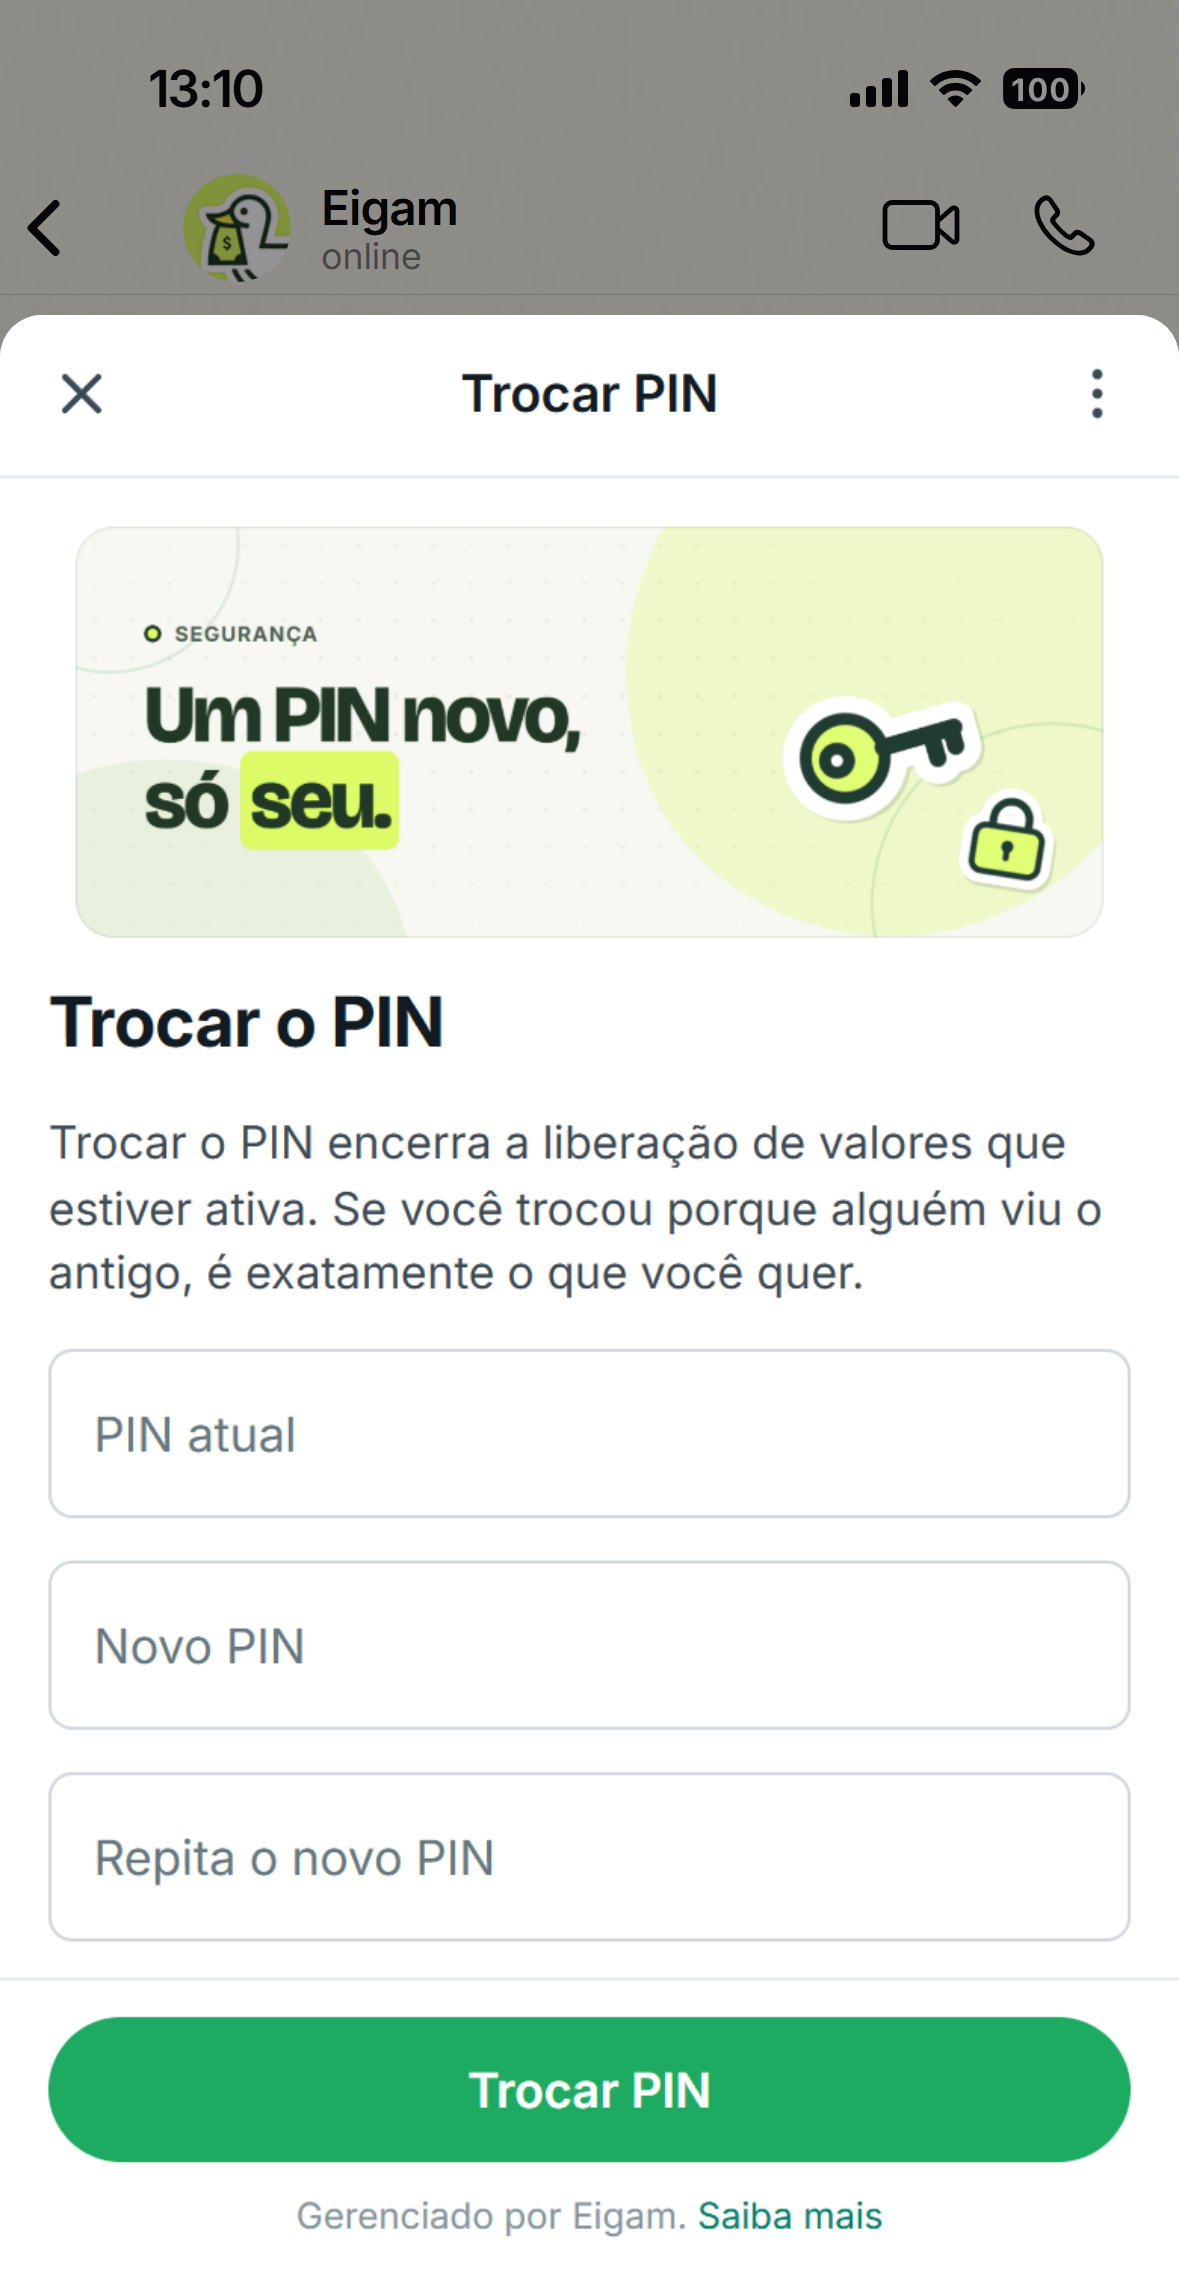
\includegraphics[width=\textwidth]{images/resultados/fluxos/fluxo_flows_b.png}
    \end{minipage}\hfill
    \begin{minipage}[t]{0.32\textwidth}
        \centering
        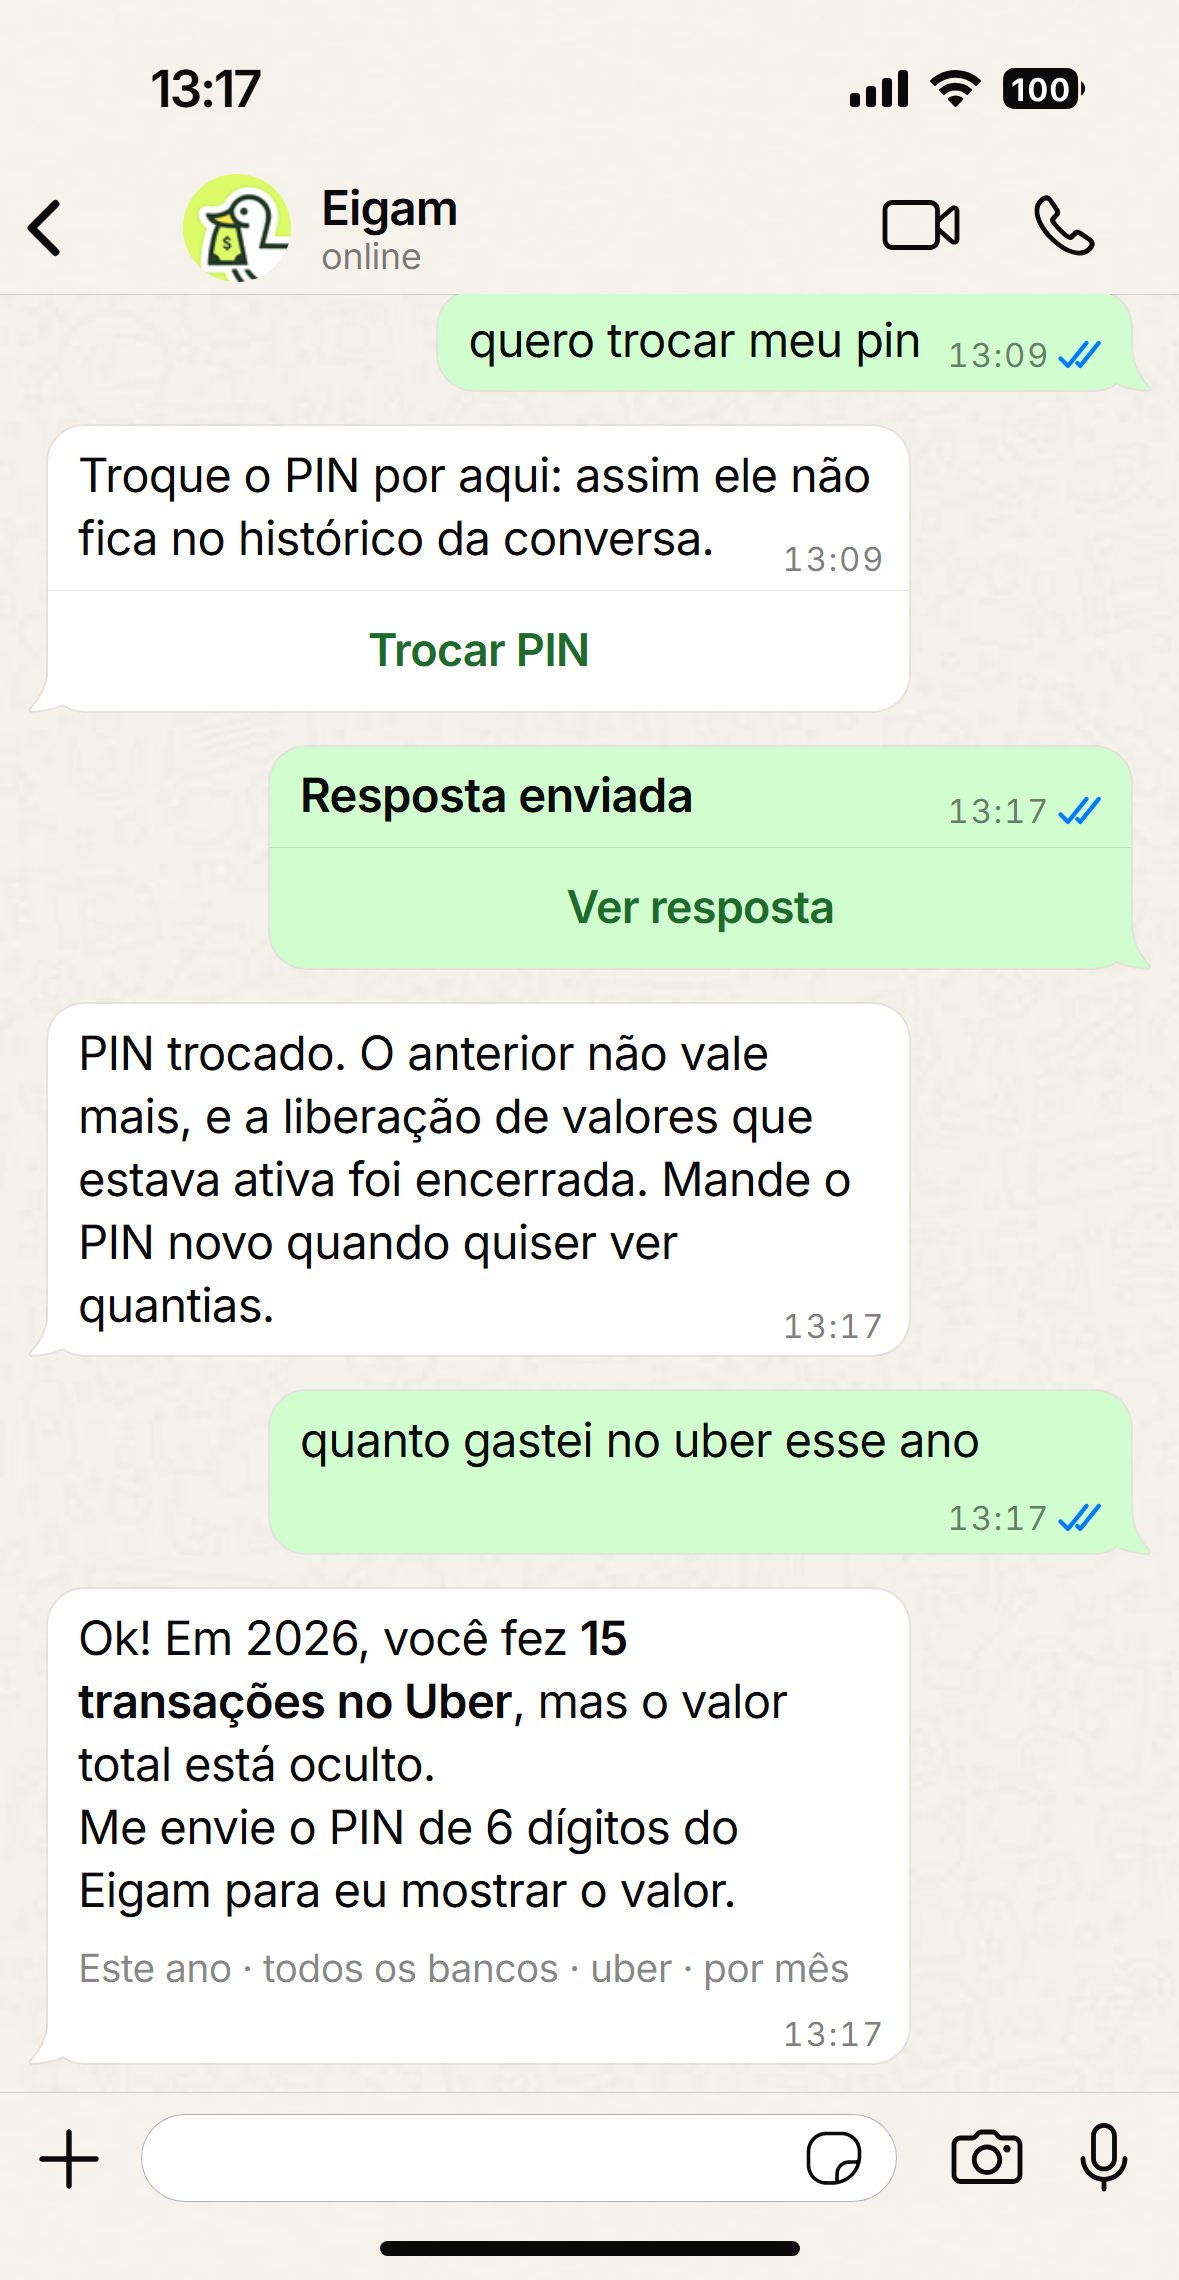
\includegraphics[width=\textwidth]{images/resultados/fluxos/fluxo_flows_c.png}
    \end{minipage}
    \authorssource
\end{figure}

\subsection{Painel do Titular}

O painel do titular não estava previsto na proposta original, que propunha uma experiência exclusivamente conversacional. Ele foi incorporado porque a conversa responde bem a perguntas curtas e mal a três necessidades: listas longas, como todas as transações do mês; visão consolidada, sem perguntar parte por parte; e gestão com confirmação visual, como bancos conectados, assinatura e privacidade. Para não contrariar a proposta, adotou-se a regra de que nada existe apenas no painel: ele estende a conversa. A Figura~\ref{fig:res_painel_inicio} mostra a tela inicial.

\begin{figure}[H]
    \centering
    \caption{Tela inicial do painel do titular}
    \label{fig:res_painel_inicio}
    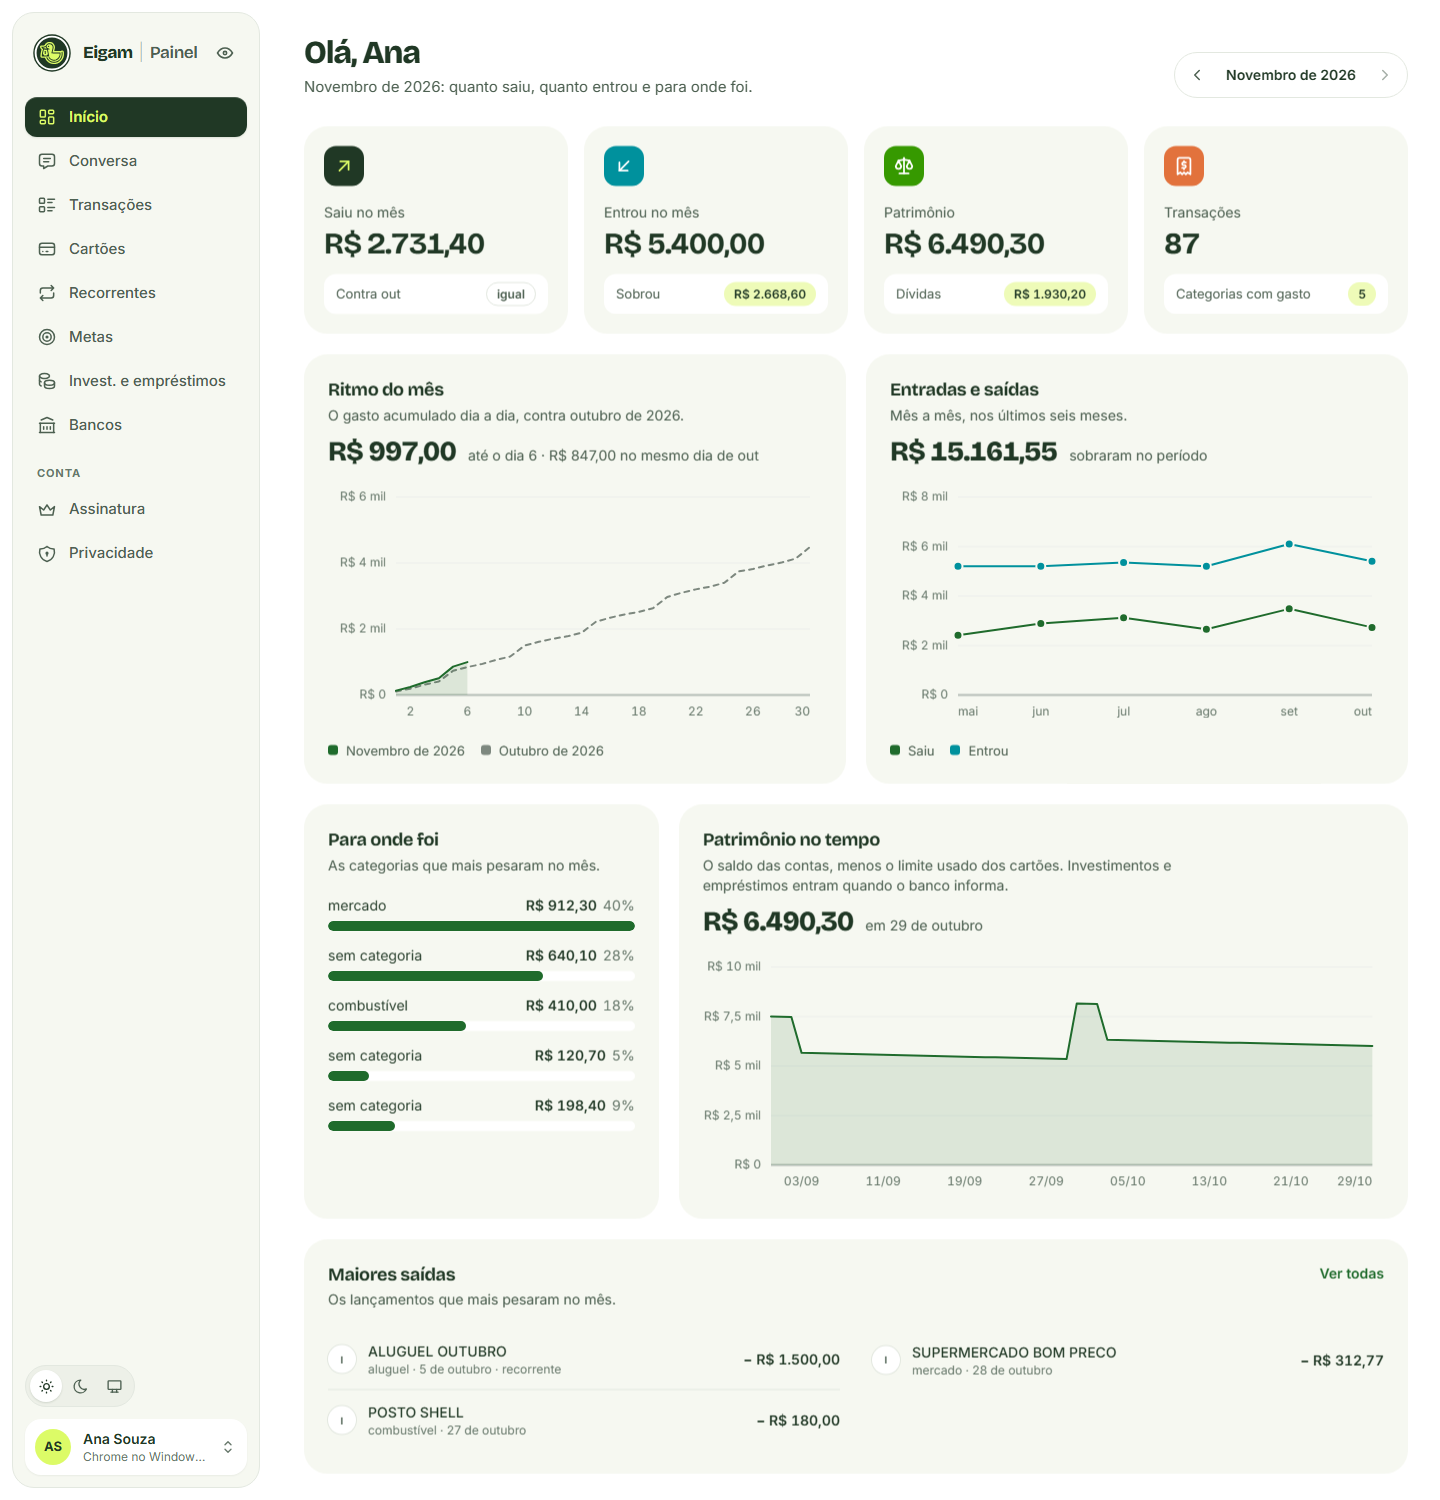
\includegraphics[width=0.95\textwidth]{images/resultados/painel_inicio.png}
    \authorssource
\end{figure}

A tela inicial resume o mês em quatro números (saídas, entradas, patrimônio e quantidade de transações) e em quatro gráficos: o ritmo do gasto comparado ao mês anterior, as entradas e saídas dos últimos seis meses, as categorias que mais pesaram e a evolução do patrimônio. A Figura~\ref{fig:res_painel_sem_pin} mostra a mesma tela sem o token de privilégio. Nesse caso, o \textit{Finance Service} devolve os valores nulos, e o painel nunca recebe o número: os gráficos de valor mostram um cadeado, e as categorias passam a ser comparadas pela quantidade de transações. O PIN digitado no painel é o mesmo da conversa e libera os valores nos dois lugares.

\begin{figure}[H]
    \centering
    \caption{Tela inicial do painel do titular sem o token de privilégio}
    \label{fig:res_painel_sem_pin}
    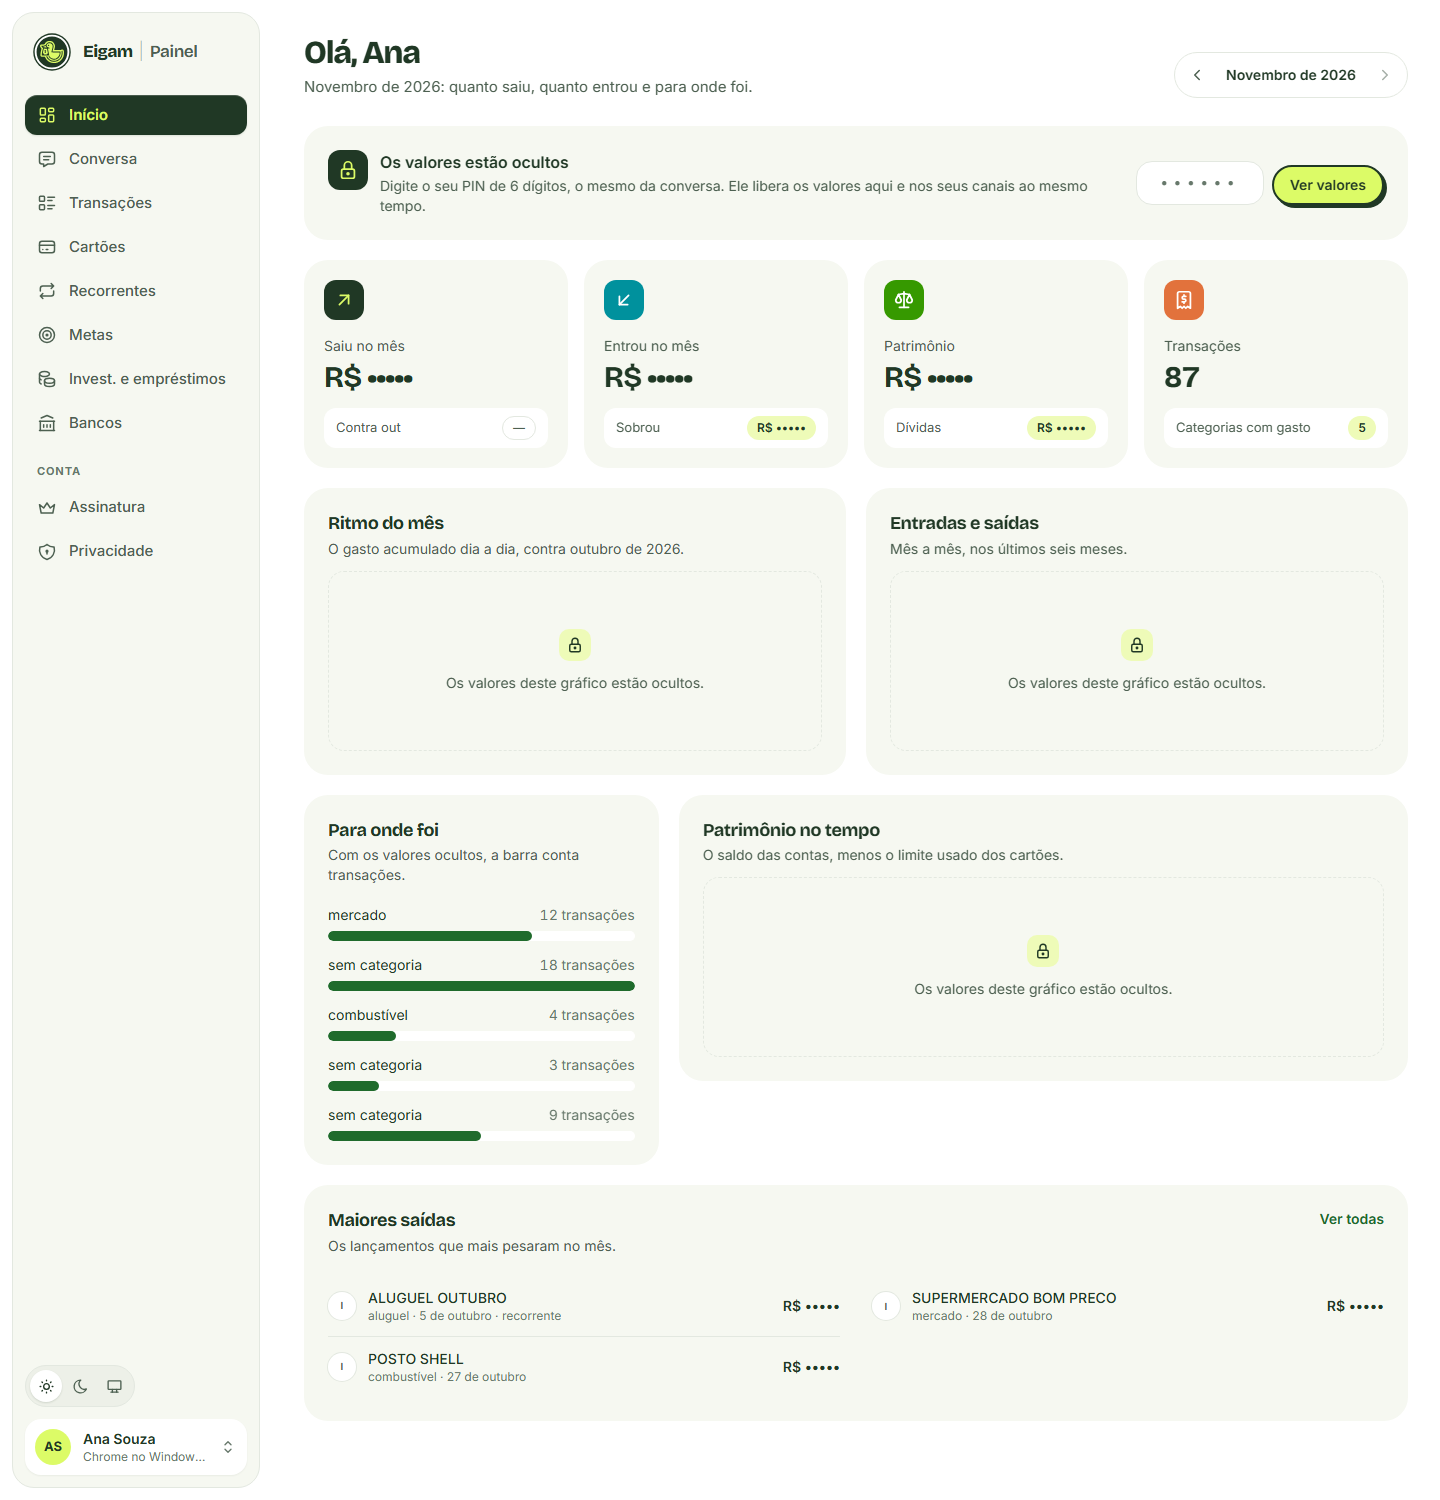
\includegraphics[width=0.95\textwidth]{images/resultados/painel_inicio_sem_pin.png}
    \authorssource
\end{figure}

As Figuras~\ref{fig:res_painel_cartoes} e~\ref{fig:res_painel_bancos} mostram duas telas de consulta longa. A de cartões reúne as faturas de todos os cartões conectados, o limite disponível e as parcelas já comprometidas nos próximos meses. A de bancos mostra, para cada conexão, a última sincronização, os saldos e o que aquela instituição informa ou não pelo \textit{Open Finance}, como investimentos e empréstimos. Essa transparência foi necessária porque a ausência de um dado nem sempre significa que ele não existe: muitas vezes o banco apenas não o informa.

\begin{figure}[H]
    \centering
    \caption{Cartões no painel do titular}
    \label{fig:res_painel_cartoes}
    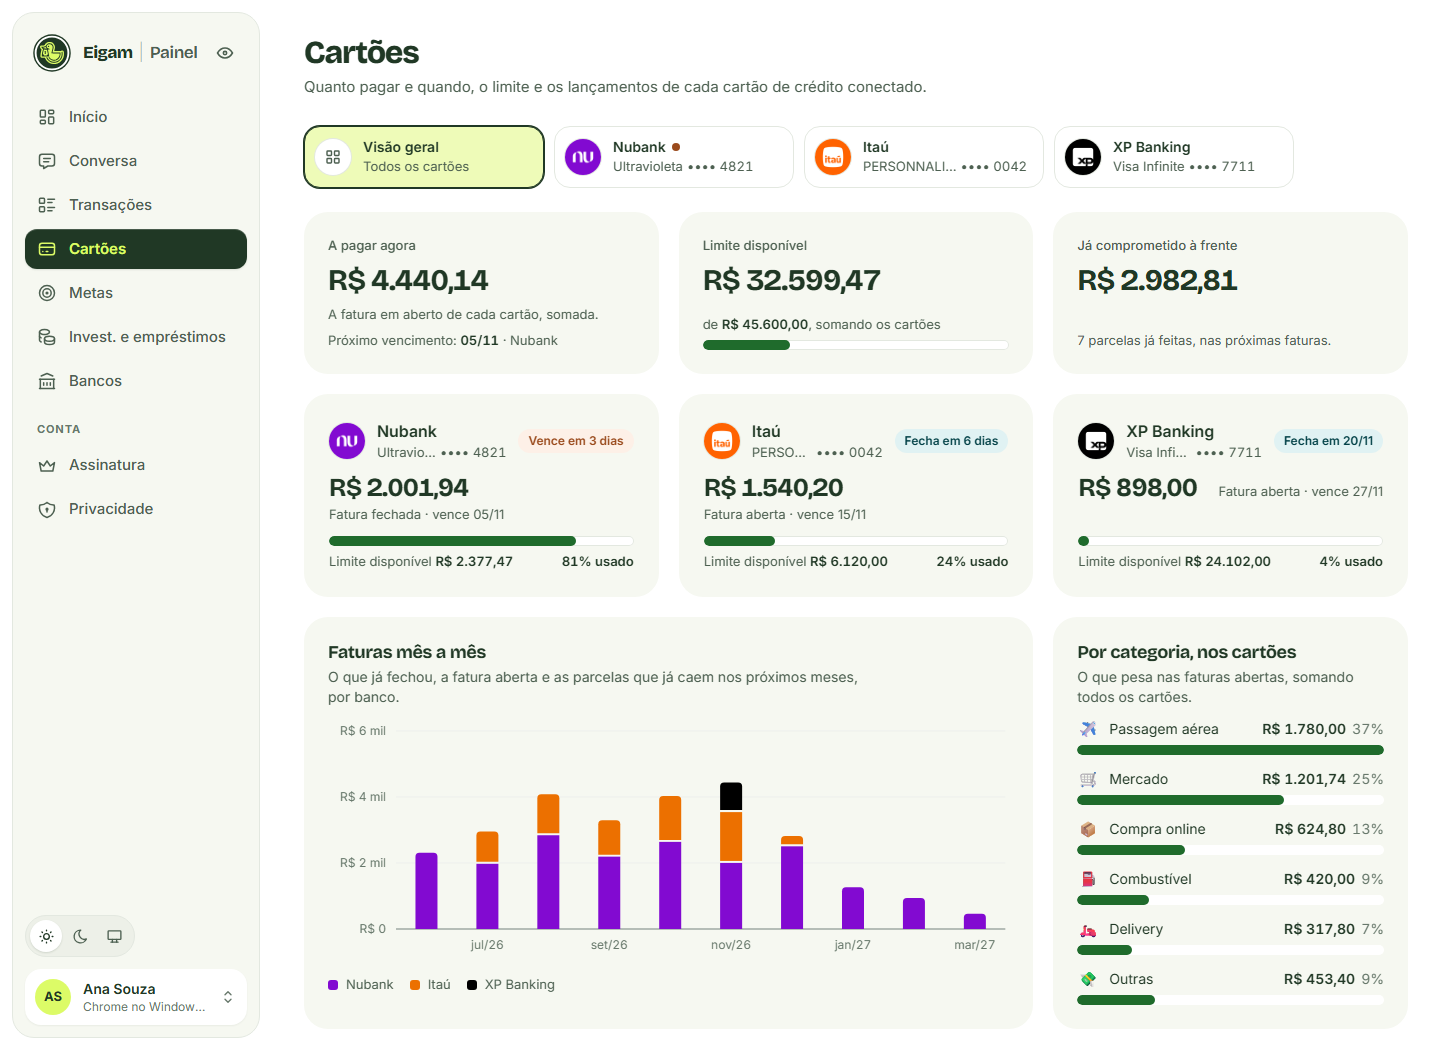
\includegraphics[width=0.95\textwidth]{images/resultados/painel_cartoes.png}
    \authorssource
\end{figure}

\begin{figure}[H]
    \centering
    \caption{Bancos conectados no painel do titular}
    \label{fig:res_painel_bancos}
    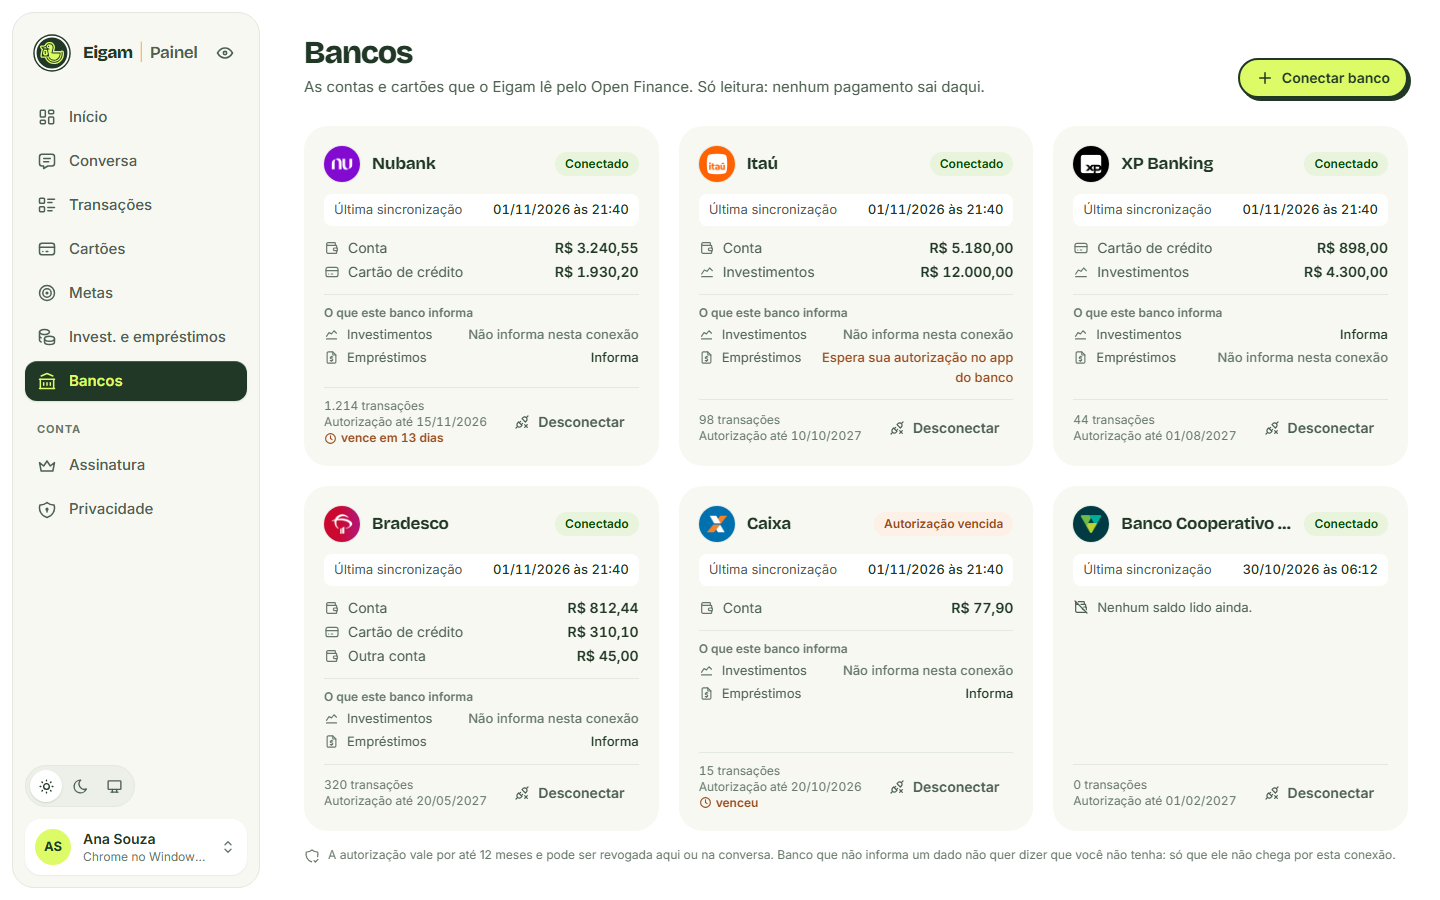
\includegraphics[width=0.95\textwidth]{images/resultados/painel_bancos.png}
    \authorssource
\end{figure}

A tela de privacidade (Figura~\ref{fig:res_painel_privacidade}) mostra os dados guardados, sem revelar o CPF, que permanece cifrado, e lista os aparelhos em que o painel está aberto. Os botões de direitos não executam nada na tela: abrem a conversa com o comando já escrito, para que a exportação e a exclusão continuem passando pelo mesmo reconhecimento determinístico e pela mesma confirmação.

\begin{figure}[H]
    \centering
    \caption{Privacidade no painel do titular}
    \label{fig:res_painel_privacidade}
    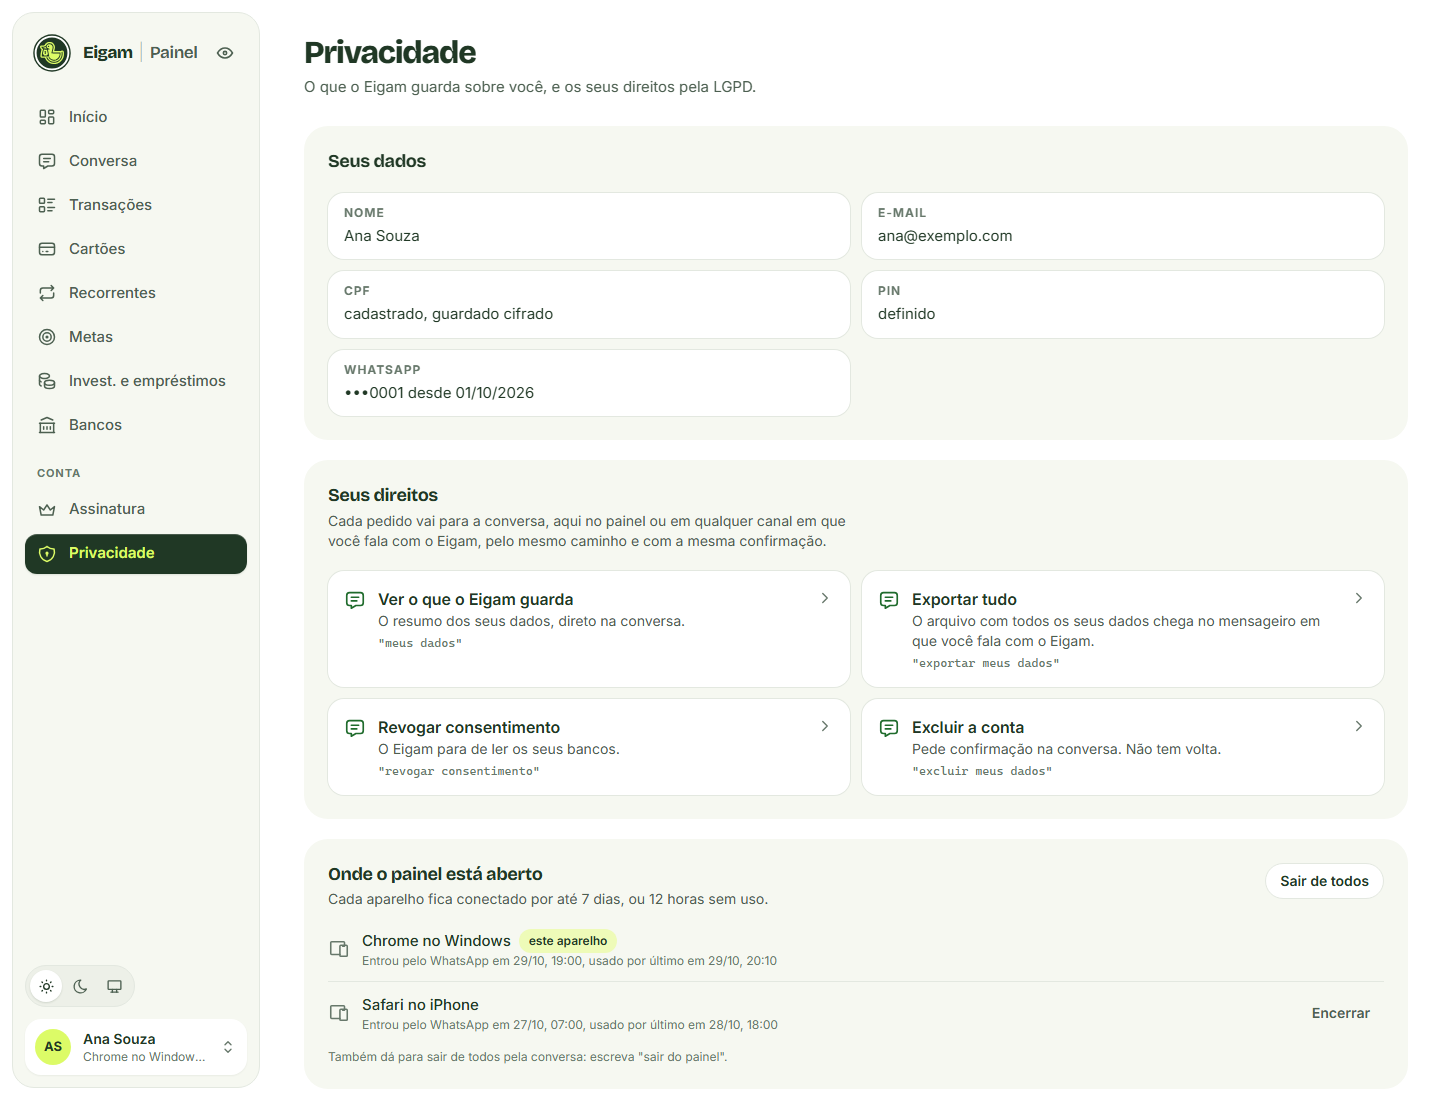
\includegraphics[width=0.95\textwidth]{images/resultados/painel_privacidade.png}
    \authorssource
\end{figure}

\subsection{Painel de Operação}

O painel de operação atende ao requisito RF012 e respondeu a necessidades que surgiram com o sistema em funcionamento: saber onde as pessoas param no cadastro sem consultar o banco de dados, ler uma conversa quando o titular pede ajuda e acompanhar o custo de cada resposta. A Figura~\ref{fig:res_operacao} mostra a visão geral, com o custo por dia separado por fonte (modelo de linguagem, mensagens do canal, verificação das respostas e transcrição de áudio), as sessões iniciadas, as conexões por banco, a saúde dos conectores do agregador e as revogações de consentimento.

\begin{figure}[H]
    \centering
    \caption{Visão geral do painel de operação}
    \label{fig:res_operacao}
    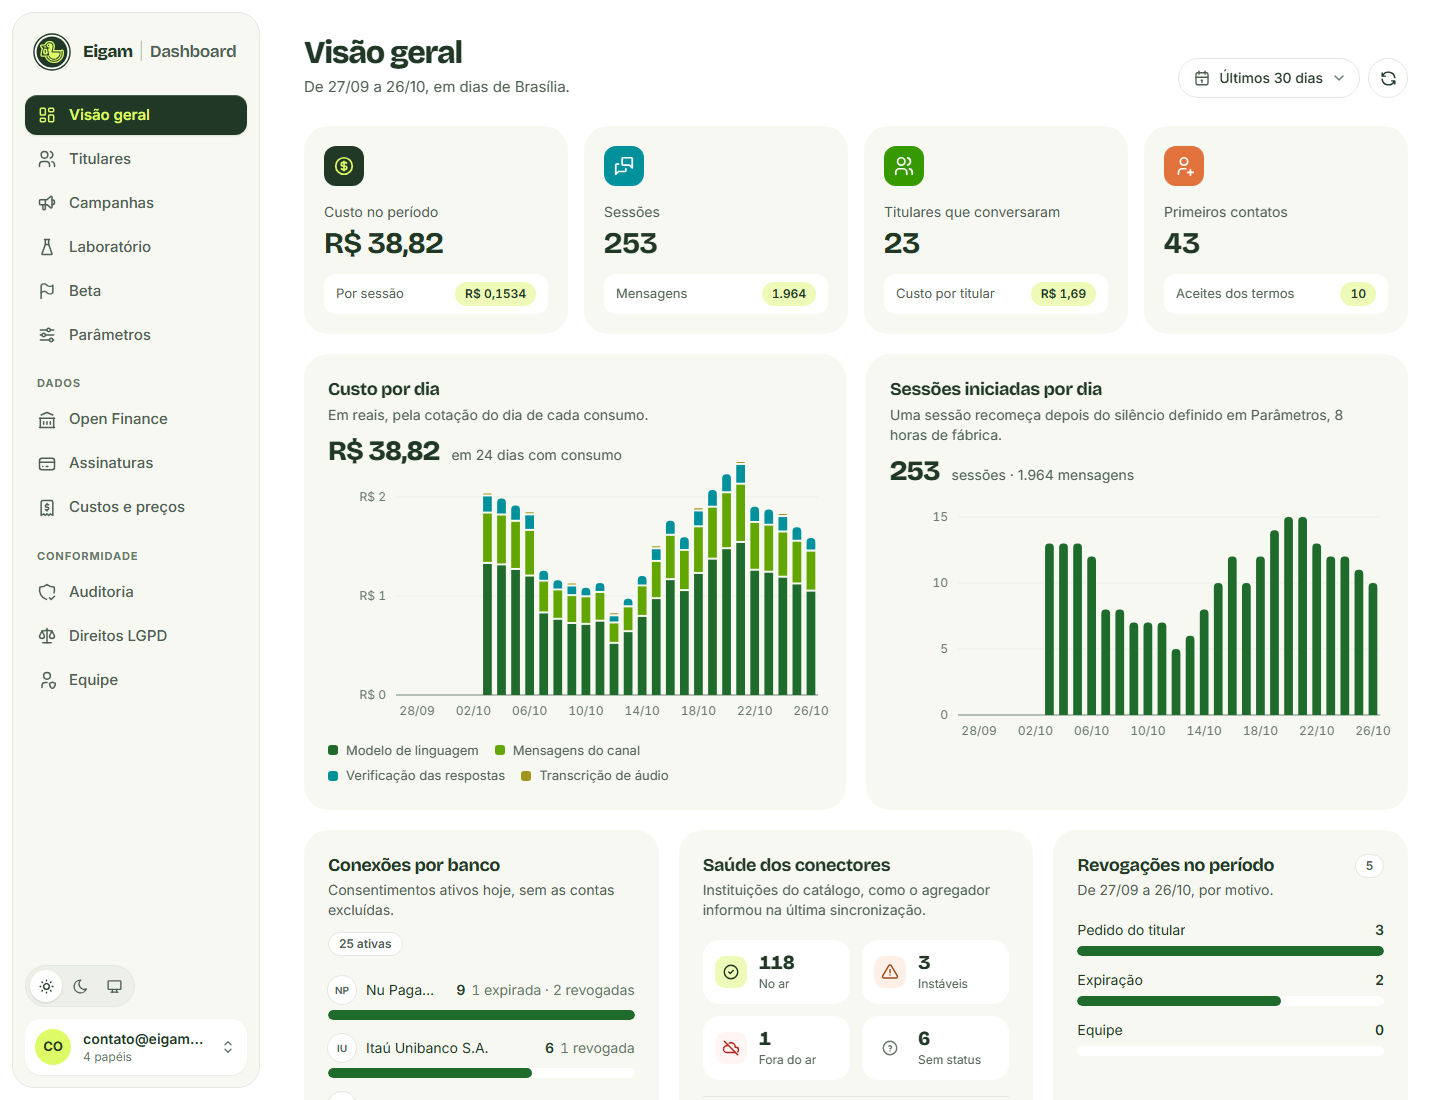
\includegraphics[width=0.95\textwidth]{images/resultados/operacao_visao_geral.png}
    \authorssource
\end{figure}

O painel não possui credencial de banco de dados: ele pede cada informação ao serviço dono pela rota interna. A leitura de conversas exige um papel específico, e é limitada a 30 titulares distintos por operador por hora.

\section{O que foi proposto e o que foi entregue}

O Quadro~\ref{frame:entregas} compara cada requisito funcional definido na fase de projeto, além do RF013, incorporado durante o desenvolvimento, com o que foi efetivamente entregue.

{\small
\begin{longtable}{|L{3.4cm}|L{2.4cm}|L{8.7cm}|}
\caption{Requisitos funcionais e o que foi entregue} \label{frame:entregas} \\
\continuesmark
\hline
\textbf{Requisito} & \textbf{Situação} & \textbf{Como foi atendido} \\ \hline
\endfirsthead
\hline
\textbf{Requisito} & \textbf{Situação} & \textbf{Como foi atendido} \\ \hline
\endhead
\endfoot
\sourcerow{3} \\
\endlastfoot
{[RF001]} Realizar cadastro & Atendido & Cadastro pela conversa no \textit{WhatsApp} ou no \textit{Telegram}, e por Mini App no \textit{Telegram}, com aceite dos termos, nome, CPF, e-mail e PIN. Antes do cadastro, é possível tirar dúvidas e experimentar o assistente com dados de demonstração. \\ \hline
{[RF002]} Vincular conta ao \textit{Open Finance} & Atendido & Conexão pelo agregador de \textit{Open Finance}, com escolha do prazo do consentimento e comprovante em imagem. \\ \hline
{[RF003]} Consultar informações financeiras & Atendido & Saldo, extrato, faturas de cartão, pagamentos recorrentes, investimentos, empréstimos e patrimônio, por qualquer recorte de período, banco, categoria, estabelecimento ou forma de pagamento, com gráficos na conversa e telas no painel. \\ \hline
{[RF004]} Gerar análises financeiras & Atendido & Comparações entre períodos com cálculo em centavos, ranking de categorias e bancos, ritmo do mês e resumos semanal e mensal em PDF. \\ \hline
{[RF005]} Gerar previsões financeiras & Atendido com ressalva & Três projeções implementadas: o gasto até o fim do mês, pelo ritmo robusto aprovado no teste retrospectivo; o gasto dos dois meses seguintes; e o saldo livre do fim do mês, que responde quanto deve sobrar nas contas. A simulação de compra mostra o efeito de uma compra hipotética sobre essas medidas. A exibição ampla depende do fechamento mensal com dados reais; até lá, as estimativas ficam atrás de chaves de liberação e o sistema declara abstenção quando os critérios estatísticos não são atingidos. \\ \hline
{[RF006]} Emitir alertas financeiros & Atendido com mudança & Seis sinais: limite de gasto em 80\% e 100\%, risco de estouro confirmado por duas previsões, possível cobrança duplicada, transação atípica e aumento por categoria, com preferências, janela de horário, entrega durável por caixa de saída transacional e autorização reconferida no instante do envio. Os alertas de vencimento e de saldo insuficiente não foram implementados como avisos; as recorrências, as faturas e a próxima cobrança podem ser consultadas na conversa e no painel. \\ \hline
{[RF007]} Fornecer recomendações personalizadas & Parcial & Observações sobre o orçamento e próximos passos sugeridos em cada resposta. Recomendações de investimento ficaram fora do escopo por decisão de produto e são bloqueadas pelos \textit{guardrails}. \\ \hline
{[RF008]} Definir metas financeiras & Atendido & Quatro tipos de meta (teto de gasto, saldo em conta, patrimônio e valor guardado), com recortes por categoria, estabelecimento, banco e forma de pagamento, criadas pela conversa ou por formulário. O valor guardado é registrado em um livro-razão cifrado e reversível, com retiradas e correções auditáveis. \\ \hline
{[RF009]} Acompanhar metas financeiras & Atendido & Progresso na conversa e no painel; tetos de gasto também geram avisos em 80\% e em 100\%. \\ \hline
{[RF010]} Gerenciar consentimento & Atendido & Consulta dos bancos conectados, revogação por mensagem ou pelo painel e encerramento automático na data escolhida. \\ \hline
{[RF011]} Gerenciar perfil & Atendido & Nome, preferências de aviso, janela de horário, troca de PIN, ocultação de valores e encerramento de sessões do painel. \\ \hline
{[RF012]} Disponibilizar painel administrativo & Atendido & Painel de operação com papéis, custos, campanhas, parâmetros, auditoria, pedidos da LGPD e laboratório. \\ \hline
{[RF013]} Disponibilizar painel do titular & Incorporado e atendido & Requisito incorporado durante o desenvolvimento: painel \textit{web} com início, conversa, transações, cartões, recorrências, metas, investimentos, bancos, assinatura e privacidade, com entrada pelo \textit{WhatsApp} e valores mascarados até o PIN. \\ \hline
\end{longtable}
}

Além do escopo original, foram entregues o \textit{Telegram} como segundo canal, o painel do titular com conversa própria (RF013), a transcrição de notas de voz, a assinatura recorrente do plano Pro, a medição do custo de cada titular, as campanhas por \textit{template}, o laboratório de respostas, a simulação de compra e o servidor MCP, que conecta o EIGAM ao assistente de inteligência artificial do próprio titular. O modelo comercial também mudou: o plano gratuito previsto na proposta foi substituído por um período de teste de sete dias, iniciado na conexão do primeiro banco e sem exigência de cartão, com os planos e preços descritos em um catálogo no \textit{Billing Service}, alterável sem nova implantação. O \textit{Telegram} foi especialmente importante para a proposta: a arquitetura multicanal deixou de ser uma promessa e passou a ser verificável, pois o mesmo titular conversa pelos três canais com o mesmo cadastro, o mesmo PIN e as mesmas respostas. O servidor MCP estendeu essa verificação para fora do produto: as mesmas rotas de leitura do painel atendem um assistente externo, com as mesmas regras de máscara e auditoria decididas no servidor.

Três decisões da modelagem foram revistas depois de medidas com dados reais. A primeira foi o Prophet, previsto para projeções com sazonalidade: na série de um titular com seis meses e 2.485 transações, seus intervalos de previsão ficaram de três a dez vezes mais largos que os da EWMA, chegando a mais de 50 vezes o próprio valor projetado, porque o gasto pessoal por categoria é esparso. A biblioteca foi removida. A segunda foi o classificador de intenções com limiares de confiança: ele foi substituído por um planejador que escolhe consultas tipadas, eliminando duas leituras divergentes da mesma frase. A terceira foi a categorização por modelo de linguagem: a categoria atribuída pelo próprio agregador de \textit{Open Finance}, mais detalhada do que as dez categorias previstas, tornou o modelo desnecessário nessa etapa. Em sentido oposto, o RAG por similaridade vetorial sobre o histórico financeiro, previsto na modelagem inicial, não chegou a ser ligado: os fatos passaram a vir de consultas estruturadas escolhidas pelo planejador, que dão o valor exato em vez de um trecho parecido, e a recuperação ficou restrita à base de conhecimento sobre o produto. Uma quarta revisão ocorreu dentro da própria política de projeção: o ritmo atual do mês, que servia de método de reserva quando nenhum candidato era aprovado, passou a ser avaliado pelos mesmos critérios dos demais e foi reprovado; a reserva escondia o pior candidato, e ``nenhum método'' passou a ser um veredito legítimo.

Em relação à pesquisa apresentada no Capítulo 3, as funcionalidades de maior interesse foram atendidas em graus diferentes. Os resumos automáticos de gastos, a mais pedida (32 de 42 respondentes), foram entregues. A detecção de gastos atípicos (21) foi entregue, junto com a de cobranças duplicadas. Os alertas de vencimento (29) foram substituídos pela consulta às recorrências e à próxima cobrança, e a previsão de saldo (26) foi atendida pelo saldo livre do fim do mês, que responde quanto deve sobrar nas contas conectadas, com liberação condicionada à medição com dados reais. A preocupação com privacidade, alta para 69\% dos respondentes, orientou o mascaramento, o PIN, a cifragem por campo e o exercício de todos os direitos por mensagem.

\section{Medição da qualidade}

A qualidade foi medida em quatro frentes: testes automatizados, avaliação da camada de inteligência artificial, desempenho e precisão das projeções. Os resultados a seguir vêm dos relatórios de validação e dos pacotes de evidência versionados no repositório de documentação do projeto.

\subsection{Testes Automatizados e Integração Contínua}

Antes de liberar os alertas, as metas e a projeção, a equipe executou as suítes completas de doze serviços. A Tabela~\ref{tab:testes} apresenta o resultado dessa validação.

\begin{tabela}[H]
\centering
\caption{Testes automatizados por serviço na validação de liberação}
\label{tab:testes}
\begin{tabular}{lrr}
\toprule
\textbf{Serviço} & \textbf{Testes aprovados} & \textbf{Cobertura de linhas} \\
\midrule
\textit{Chat Service} & 4.423 & 95,23\% \\
\textit{AI Service} & 1.931 & não medida \\
\textit{Finance Service} & 1.678 & 91,38\% \\
\textit{Identity Service} & 859 & 90,42\% \\
Pacote compartilhado (\textit{shared}) & 696 & 93,67\% \\
\textit{Outbound Worker} & 413 & 94,11\% \\
Painel de operação & 328 & 93,92\% \\
\textit{API Gateway} & 306 & 92,77\% \\
\textit{Billing Service} & 250 & 92,14\% \\
\textit{Notification Service} & 228 & 87,42\% \\
Painel do titular & 155 & 93,52\% \\
\textit{Analytics Service} & 82 & 93,25\% \\
\bottomrule
\end{tabular}
\authorssource
\end{tabela}

A primeira execução encontrou 11.317 testes aprovados e 2 reprovados, além de sete defeitos funcionais revelados por provas dirigidas com bancos reais e com o fluxo integrado. Entre eles estavam uma corrida que permitia criar mais metas do que o plano então vigente admitia e uma projeção calculada no fuso horário errado na virada do mês. Os sete defeitos foram corrigidos com 30 testes novos. Os quatro serviços alterados foram reexecutados, com 6.411 testes aprovados e nenhum reprovado, e os números da tabela já refletem essa reexecução. A cobertura ficou entre 87\% e 95\%, acima do mínimo de 70\% exigido pela integração contínua. O \textit{Render Service} e o \textit{Audit Service}, que não fizeram parte dessa validação, também possuem suítes próprias executadas pela integração contínua.

A reconstrução de metas, alertas e predição ampliou essas suítes: ao final da integração, a suíte do \textit{Finance Service} passava de 2.000 testes, com dezenas de verificações de integração executadas contra PostgreSQL, MongoDB e Redis reais, incluindo interrupções forçadas do processo (SIGKILL) após confirmações de escrita, para provar que travas, diários de intenção e recuperação administrativa deixam o banco em estado consistente. A auditoria adversarial dessa frente registrou dezoito achados, cada um com estado sustentado e condição restante documentados em uma matriz de liberação; a jornada completa em canal real permaneceu como portão final antes da exposição ao público.

\subsection{Camada de Inteligência Artificial}

A Tabela~\ref{tab:golden} apresenta os resultados dos principais \textit{golden sets}. Os conjuntos que dependem apenas de regras determinísticas atingiram 100\%, como exigido. Os que dependem do modelo foram medidos em baterias com o modelo real.

\begin{tabela}[H]
\centering
\caption{Resultados dos principais \textit{golden sets}}
\label{tab:golden}
{\small
\begin{tabular}{L{6.3cm}rr}
\toprule
\textbf{Conjunto} & \textbf{Casos} & \textbf{Resultado} \\
\midrule
Mascaramento de valores sem token & 98 & 100\% \\
Comandos da LGPD (revocação e precisão) & 174 & 100\% \\
Ações sobre bancos & 155 & 100\% \\
Leitura de metas por regra & 221 & 100\% \\
\textit{Guardrail} de conselho e credencial & 127 & 100\% \\
Conselhos sem produto citado (fora do treino) & 20 & 20/20 \\
\textit{Prompt injection} (30 ataques e 43 frases legítimas) & 73 & 73/73 \\
Leitura do cadastro pelo planejador & 172 & 172/172 \\
Motivo da frase pelo planejador (Macro-F1) & 348 & 0,914 \\
Consultas financeiras sem data ou banco errados & 1.512 & 100\% \\
\bottomrule
\end{tabular}
}
\authorssource
\end{tabela}

A conformidade de 100\% no mascaramento e nos comandos da LGPD era a meta inegociável do projeto, porque um valor exposto ou um pedido de exclusão perdido causariam dano real ao titular. Ambos são decididos por regras determinísticas, e não pelo modelo, o que torna o resultado reprodutível. O \textit{guardrail} de conselho mostra por que a combinação de regra e modelo foi necessária. A expressão regular sozinha bloqueou apenas 10 dos 20 conselhos do conjunto mantido fora do desenvolvimento, que eram escritos sem citar produto financeiro, como ``deixar esse dinheiro parado na conta perde da inflação''. O modelo de juízo bloqueou os 20, com mediana de 267~ms. Na \textit{prompt injection}, a expressão regular sozinha detectou 20 dos 30 ataques; com o juízo, os 30.

No conjunto de 1.512 consultas financeiras, nenhuma frase gerou data ou banco errados. O Macro-F1 de 0,914 na identificação do motivo da frase ficou acima do mínimo de 0,88 definido.

Para avaliar respostas abertas, foram geradas perguntas complexas, parte escritas pela equipe e parte por um modelo de linguagem sem acesso às regras do sistema. Um segundo modelo, atuando como juiz, atribuiu notas de 0 a 10 a cada resposta produzida pelo turno completo em produção. A Tabela~\ref{tab:complexas} apresenta a evolução das notas médias entre a primeira e a última medição, depois das correções.

\begin{tabela}[H]
\centering
\caption{Notas médias das respostas a perguntas complexas}
\label{tab:complexas}
\begin{tabular}{lrrr}
\toprule
\textbf{Conjunto} & \textbf{Perguntas} & \textbf{Primeira medição} & \textbf{Última medição} \\
\midrule
Escrito pela equipe & 153 & 8,20 & 9,03 \\
Gerado 1 & 176 & 7,60 & 8,49 \\
Gerado 2 & 154 & 7,75 & 8,18 \\
Gerado 3 & 154 & 7,32 & 7,71 \\
Gerado 4, nunca usado para corrigir & 154 & -- & 8,53 \\
Perguntas difíceis & 77 & 7,27 & 8,23 \\
\bottomrule
\end{tabular}
\authorssource
\end{tabela}

O conjunto 4 é o resultado mais relevante da tabela. Como nunca foi usado para orientar correções, ele mede a generalização, e a nota de 8,53 indica que as melhorias não foram ajustadas apenas às perguntas já conhecidas. O ponto mais fraco identificado foi o orçamento, com notas entre 6,5 e 6,9. Na bateria final de perguntas difíceis, nenhuma resposta trouxe valor em reais fora dos fatos consultados.

\subsection{Desempenho e Capacidade}

O teste de carga foi executado no próprio servidor de produção, ao lado do sistema em uso, em uma rede isolada, sem acesso ao provedor do modelo de linguagem, aos canais de mensageria nem ao agregador de \textit{Open Finance}, e sem tocar em dados de titulares. Um modelo simulado devolvia os planos reais gravados de 1.512 frases, com o tempo real de cada chamada, e as mensagens chegavam segundo um processo de Poisson. A Tabela~\ref{tab:carga} resume os resultados, em segundos, do recebimento do \textit{webhook} até o envio ao canal.

\begin{tabela}[H]
\centering
\caption{Latência no teste de carga antes e depois da mudança de consumidores}
\label{tab:carga}
{\small
\begin{tabular}{lrrrr}
\toprule
\textbf{Configuração} & \textbf{Mensagens/s} & \textbf{Usuários equivalentes} & \textbf{p50} & \textbf{p95} \\
\midrule
Original & uma por vez & -- & 5,0 & 7,0 \\
Original & 0,2 & 570 & 5,5 & 9,6 \\
Original & 1,0 & 2.850 & 51,9 & 82,4 \\
Um consumidor por partição & 0,2 & 570 & 5,0 & 7,1 \\
Um consumidor por partição & 1,0 & 2.850 & 6,1 & 10,3 \\
Um consumidor por partição & 3,0 & 8.600 & 8,5 & 22,7 \\
\bottomrule
\end{tabular}
}
\authorssource
\end{tabela}

O teste revelou que o limite não estava na máquina: a CPU não passou de 51\% em nenhuma rodada. O gargalo era o cliente Kafka do \textit{Chat Service}, que buscava um lote de mensagens e só buscava o seguinte quando todas terminassem. Assim, uma resposta que esperava o modelo por cinco segundos segurava a mensagem de outro titular. Com doze partições e um consumidor por partição, o ritmo sustentado passou de 0,6 para 2,9 mensagens por segundo, e a capacidade com boa experiência passou de cerca de 570 para cerca de 2.850 usuários no mesmo servidor de 4 vCPU. A conversão para usuários usa a referência de projeto de dez mensagens por dia por usuário, com pico de três vezes a média. O pico real observado nas horas anteriores ao teste foi de 0,0064 mensagem por segundo, cerca de 3\% da nova capacidade.

Quanto à latência percebida, o \textit{gateway} respondeu às rajadas de até 100 \textit{webhooks} por segundo com p99 de no máximo 12~ms, aplicando o limite de taxa acima de 50 requisições por segundo, o que atende à regra de responder imediatamente ao provedor. No caminho completo, as medianas foram de 1,97~s no planejador, 2,6~s na redação e 0,3~s nas consultas financeiras. A mensagem isolada levou 5,0~s na mediana, e as perguntas complexas, entre 4,3 e 5,0~s. Esses tempos ficaram acima da meta de cerca de 4 segundos definida no projeto. A espera é parcialmente mascarada pelo indicador de digitação, que aparece em cerca de 30~ms, mas reduzir o tempo da redação é a principal melhoria de desempenho pendente.

\subsection{Projeções e Saldo Livre}

A projeção foi o requisito em que a medição mais alterou a proposta, em duas rodadas. A Tabela~\ref{tab:prophet} mostra a largura do intervalo de previsão de 80\%, como percentual do valor projetado, medida na série real de um titular com seis meses de histórico. O modelo de dados define que uma projeção só é confiável quando essa largura não ultrapassa 40\%.

\begin{tabela}[H]
\centering
\caption{Largura do intervalo de previsão como percentual do valor projetado}
\label{tab:prophet}
\begin{tabular}{lrr}
\toprule
\textbf{Série} & \textbf{Prophet} & \textbf{EWMA} \\
\midrule
Alimentação, semanal & 2.082\% & 433\% \\
Contas fixas, semanal & 1.060\% & 110\% \\
Transporte, semanal & 5.406\% & 180\% \\
Total, semanal & -- & 91\% \\
\bottomrule
\end{tabular}
\authorssource
\end{tabela}

Diante desse resultado, a projeção passou a estimar o gasto até o fim do mês corrente, no total ou por categoria, com os métodos candidatos escolhidos por teste retrospectivo. A primeira rodada, com três candidatos, reprovou todos: a mediana histórica acertava o centro, mas cobria o valor real em apenas 27\% dos casos, e a EWMA tinha viés de 12\%. A investigação dessa reprovação revelou um problema na própria política: o ritmo atual do mês era usado como reserva sempre que ninguém passava, sem ser confrontado com os mesmos critérios, e era o pior candidato. A política foi então refeita: todos os candidatos, inclusive o ritmo atual, passaram a ser julgados pelos mesmos critérios, ``nenhum método'' virou um veredito válido, e um novo candidato foi construído, o ritmo robusto, que estende aos dias restantes apenas o gasto típico, com a régua de dia atípico tirada do histórico. A Tabela~\ref{tab:backtest} apresenta o teste retrospectivo final, sobre oito séries sintéticas com 426 origens e corte no dia 15, incluindo cenários adversos como uma compra pontual de R\$~5.000, um aluguel no dia 3 e duas semanas de viagem.

\begin{tabela}[H]
\centering
\caption{Teste retrospectivo da projeção de fim de mês}
\label{tab:backtest}
{\small
\begin{tabular}{lrrrr}
\toprule
\textbf{Método} & \textbf{WAPE} & \textbf{Viés} & \textbf{Cobertura 80\%} & \textbf{Abstenções} \\
\midrule
Ritmo atual do mês & 33,3\% & +29,3\% & 89,1\% & 0/71 \\
Mediana do restante & 5,6\% & $-$0,6\% & 87,0\% & 24/71 \\
EWMA & 19,9\% & +16,3\% & 77,5\% & 7/71 \\
Ritmo calibrado & 11,5\% & +9,2\% & 77,3\% & 25/71 \\
\textbf{Ritmo robusto} & \textbf{4,6\%} & \textbf{+0,1\%} & \textbf{89,1\%} & \textbf{0/71} \\
Mistura & 18,6\% & +15,4\% & 87,0\% & 24/71 \\
Último mês & 13,7\% & +1,6\% & 76,9\% & 8/71 \\
\midrule
Critério de aprovação & $\leq$ 20\% & $\leq$ 5\% & 70\% a 90\% & -- \\
\bottomrule
\end{tabular}
}
\authorssource
\end{tabela}

O ritmo robusto venceu com folga: empata com o ritmo atual nas séries sem dia atípico e erra muito menos nas demais, como no cenário do aluguel (0,8\% contra 71,9\%). Nas séries reais de três titulares internos, obtidas pela exportação da LGPD, os meses comuns passaram no critério (WAPE de 12,6\%), e o erro se concentrou nos meses com compra grande fora do padrão, que nenhum histórico antecipa; um candidato que decompõe o mês em compromissos conhecidos e gasto variável roda em sombra no registro de previsões como possível substituto. O veredito sintético, porém, não libera nada sozinho: a estimativa só chega ao público geral depois de aprovada no fechamento mensal com dados reais, e até lá fica disponível apenas para os usuários do beta, apresentada como experimental e com critério de desligamento escrito.

O saldo livre do fim do mês foi avaliado da mesma forma. No dado real de um titular interno, com nove meses de histórico, o desenho final errou na mediana 1,7\% da renda mensal, com viés de $-$1,9\% e faixa cobrindo todos os meses; o desenho anterior, que somava apenas a renda regular, tinha viés de $-$9,1\% e cobertura nula, e foi descartado. Em uma base bancária pública com 4.500 contas e 162 mil origens, contar toda entrada em conta, em vez de só a renda, reduziu o viés de +4,5\% para +1,3\% da renda e elevou a cobertura da faixa de 31\% para 58\%, ainda abaixo da régua de 70\% a 90\%, o que mantém a liberação condicionada ao primeiro fechamento mensal com os usuários do beta. A abstenção continua sendo uma escolha deliberada: um assistente que mostra ``R\$ 4.312,57'' com duas casas decimais transmite uma confiança que os dados não sustentam, e a pesquisa mostrou que a confiança em assistentes de IA para finanças ainda é frágil.

\subsection{Custo de Operação}

O custo de cada resposta passou a ser medido pelo próprio sistema: os serviços publicam as unidades consumidas (\textit{tokens}, mensagens cobradas, conexões bancárias e cobranças de cartão) e o \textit{Billing Service} converte esses valores em reais pela cotação do Banco Central. A infraestrutura completa, com quatorze serviços, bancos, \textit{broker} e observabilidade, custou cerca de 12 euros por mês. Cada chamada ao planejador custou entre R\$~0,016 e R\$~0,019, e o modelo de juízo dos \textit{guardrails} acumulou R\$~0,30 em pouco mais de duas semanas de uso, o que corresponde a um custo estimado de US\$~0,0009 por usuário por mês no \textit{guardrail} de conselho regulado.

A medição também corrigiu uma premissa da análise de viabilidade. O maior custo variável não é a infraestrutura nem o modelo de linguagem, mas a conexão bancária, cobrada por conexão ativa, e as mensagens do \textit{WhatsApp}, cobradas uma a uma. A regra de uma mensagem por interação reduziu diretamente esse custo, e a decisão de manter o \textit{Telegram} como canal alternativo ganhou também um argumento econômico, já que o envio de mensagens por ele não é cobrado.

\section{Limitações}

Os resultados devem ser lidos com as seguintes limitações. O beta tem poucos titulares e poucos meses de histórico, o que impede medir satisfação, retenção e o efeito do produto sobre o comportamento financeiro. O sistema roda em um único servidor, chamado de ambiente de desenvolvimento, mas usado como produção; a separação em servidores dedicados está planejada e não foi executada.
